%\documentclass[keele]{kthesis}
\documentclass[keele,double]{kthesis}

%
% We need this package to define the bibliography title later on.
%
\usepackage{authordate1-4}
\usepackage{listings}

\lstset{
  language=python,                % choose the language of the code
  numbers=left,                   % where to put the line-numbers
  stepnumber=1,                   % the step between two line-numbers.        
  numbersep=5pt,                  % how far the line-numbers are from the code
  backgroundcolor=\color{white},  % choose the background color. You must add \usepackage{color}
  showspaces=false,               % show spaces adding particular underscores
  showstringspaces=false,         % underline spaces within strings
  showtabs=false,                 % show tabs within strings adding particular underscores
  tabsize=2,                      % sets default tabsize to 2 spaces
  captionpos=b,                   % sets the caption-position to bottom
  breaklines=true,                % sets automatic line breaking
  breakatwhitespace=true,         % sets if automatic breaks should only happen at whitespace
  title=\lstname,                 % show the filename of files included with \lstinputlisting;
}

%
% Use the \usepackage{<package name>} command here to enable extra
% features that the standard LaTeX implementation doesn't provide.
% For example the citation style file, extra mathematical capabilities.
%



%\usepackage{epstopdf}
\usepackage{keele_cite}
\usepackage{latexsym}
\usepackage{amsmath}
\usepackage{amsfonts}
\usepackage{theorem}
\usepackage{graphicx}
\usepackage{epstopdf}
\graphicspath{ {Images/} }
\usepackage{pdfpages}
\usepackage{txfonts}
\usepackage{braket}
\usepackage{subcaption}
\captionsetup{compatibility=false}
\usepackage{braket}
\usepackage{rotating}
\usepackage{pdflscape}
\usepackage{auto-pst-pdf}

%
% Define some commonly used notations, subscripts and superscripts.
% These will vary depending on subject.
%
\newcommand{\sunM}{\mbox{\,M$_\odot$}}
\newcommand{\sunR}{\mbox{\,R$_\odot$}}
\newcommand{\sunL}{\mbox{\,L$_\odot$}}
\newcommand{\starM}{\mbox{\,M$_*$}}
\newcommand{\starR}{\mbox{\,R$_*$}}
\newcommand{\starL}{\mbox{\,L$_*$}}
%\newcommand{\mic}{\mbox{$\,\mu$m}}
%\newcommand{\arcsec}{\mbox{$''$}}
%\newcommand{\arcmin}{\mbox{$'$}}
%\newcommand{\vunit}{\mbox{\,km\,s$^{-1}$}}

%
% Setup the theorem numbering environment
%
\newtheorem{definition}{Definition}[chapter]
\newtheorem{theorem}[definition]{Theorem}
\newtheorem{lemma}[definition]{Lemma}
{\theorembodyfont{\upshape} \newtheorem{example}{Example}[chapter]}

%
% Biblography headings
%
\renewcommand{\bibtitle}{Bibliography}
\renewcommand{\bibheadtitle}{BIBLIOGRAPHY}

%
% Some other stuff   ADS 29/06/94
%
\makeatletter \renewcommand\@biblabel[1]{} \makeatother

%
% New commands following the advice of Gerry Pratt (cca13@cc.keele.ac.uk)
%
\renewcommand{\topfraction}{0.99}
\renewcommand{\bottomfraction}{0.99}
\renewcommand{\textfraction}{0.01}

%%%%%%%%%%%%%%%%%%%%%%%%%%%%%%%%%%%%%%%%%%%%%%%%%%%%%%%%%%%%%%%%%%%%%%%%%

%
% Define your thesis front matter here by filling in the commands.
%

\title{Fundamental properties of M-dwarfs in eclipsing binary star systems}
\author{Samuel Gill}
\qualifications{M.Phys. (Hons.) York}
\degree{Doctor of Philosophy}
\school{Department of Physics}
\date{October 2019}

\begin{document}

%
% Main section. Here I will add chapters which will be detailed in a comment above.
%

% Abstract
%\prechapter{Abstract}

% Introduction to mass and radius of low-mass stars
The absolute parameters of M-dwarfs in eclipsing binary systems provide important tests for evolutionary models. Those that have been measured have revealed significant discrepancies with evolutionary models. There are two problems with M-dwarfs: 1. M-dwarfs generally appear bigger and cooler than models predict (such that their luminosity agrees with models) and 2. some M-dwarfs in eclipsing binaries are measured to be hotter than expected for their mass. The exact cause of this is unclear and a variety of conjectures have been put forward including enhanced magnetic activity and spotted surfaces. However, there is a lack of M-dwarfs with absolute parameters and so the exact causes of these disparities are unclear. As the interest in low-mass stars rises from the ever increasing number of exoplanets found around them, it is important that a considerable effort is made to understand why this is so.


% The EBLM project
A solution to the problem lies with low-mass eclipsing binary systems discovered by the WASP project. A large sample these systems have been followed up with spectroscopic orbits that ultimately exclude them from the planet-hunting process. In this work I obtained follow-up photometry for 9 of these systems and used these data to measure the absolute parameters of each star. These will eventually be used to create empirical calibrations for low mass stars when the number of EBLMs measured within this framework increases.

% Spectroscopic analysis of EBLM systems
Breaking the mass degeneracy required supplementary information from evolutionary models and the primary stars atmospheric parameters. I successfully created, tested and deployed a spectral analysis routine which used wavelet decomposition to analyse the spectra of FGK stars in exoplanet/eclipsing binary systems. Careful selection of wavelet coefficients filter out large systematic trends and noise typically observed in spectra. I used this principle to reliably measure $T_{\rm eff}$, $V \sin i$ and [Fe/H] from CORALIE spectra. My method had a systematic offset in [Fe/H] of $-0.18$\,dex relative to equivalent-width measurements of higher-quality spectra. There is also a trend between $T_{\rm eff}$ and $\log g$ which has unclear origins.


% Problems with he sample
The sample of eclipsing binary systems in this work highlight that only a fraction are suitable for empirical calibrations. I found that four of systems have primary stars which have evolved into the ``blue-hook'' part of their main-sequence evolution. They have two distinct solutions for mass and age which require supplementary information before they can be used in empirical calibrations. A further two systems have large impact parameters which increase the uncertainty in radius above the required precision of a few percent. I advocate the need for a volume-limited sample to avoid spending time observing and measuring such systems.

% Problems with the method
The method used to measure low-mass eclipsing binaries is well-established, yet there is a dearth well-studied F+M binaries. The EBLM project has provided spectroscopic orbits for 118 F+M binaries and I expect the absolute parameters for these systems to follow timely. However, there is a requirement for a \textit{hare-and-hounds} style experiment to assess how absolute parameters differ between different research groups and methods of analysis. I show that subtle choices in helium-enhancement and mixing-length parameters can introduce a 2-4\% uncertainty in mass and age. A similar effect is seen for different limb-darkening laws and so an in-depth review into how this will affect empirical mass-radius calibrations is required. 


% Thanks
%\prechapter{Acknowledgements}

\begin{quote}
``{\it Results based on 12 mental health symptoms (GHQ-12) showed that 32\% of PhD students are at risk of having or developing a common psychiatric disorder, especially depression.}''

-- \citet{LEVECQUE2017868}
\end{quote}

% Pierre and Barry and Amaury
I would like to thank my primary supervisor, Pierre Maxted, for always encouraging me do science better. No Journey through research is straightforward. The journey which produced this work involved scaling many mountains, crossing many riverines and navigating the thickest fog. You patiently nudged me in the right direction to ensure I never ventured too far from the beaten track, and for that I am exceptionally grateful. I would also like to thank my second supervisor, Barry Smalley, who always had an open ear to discuss all things spectroscopy. I thank Jessica Evans, Daniel Evans, John Southworth, David Anderson and Amaury Triaud for assisting in observations which feature in this work.


% Katie and Bruce
Students in research degrees, and academia in general, face higher mental health risks than other professions. Lone working, stress and \textit{impostor syndrome} often leads to depression, guilt, isolation and negative thoughts. This often degrades ones self-confidence and the relationships with those closest to us. I would be fooling myself if I didn't acknowledge that I have experienced some, if not all of the symptoms mentioned above whilst studying for my doctorate. I would never have been able to survive my Ph.D without the endless love and support of my wife, Katie. Thank you for always bringing a smile to my face and helping me weather the harshest of storms. I  thank my parents, Jean and Simon Gill. You provided me with emotional and financial support during my research, as well as invaluable guidance. For this I am eternally grateful.

I would also like to honourably mention our beagle, Bruce McGill. Throughout my research you slept on my feet, taxed all my crunchy goods and pestered me for \textit{walkies}. Those walks provided crucial down time which helped me relax and preserved my sanity. Thank you for needing so little and doing so much. 

% Chapter 1. The problem with low-mass stars
%% Excellent overview of low-mass stars for the introduction chapters:
% https://arxiv.org/pdf/1804.04133.pdf


\chapter{Introduction}\label{chapter:introduction}


% greate review by https://arxiv.org/pdf/1610.05765.pdf
\iffalse
\begin{quote}
``{\it Only two things are infinite, the universe and human stupidity, and I'm not sure about the former.}''

-- Albert Einstein
\end{quote}
\fi

% Introduction to the M-spectral type
When you observe the night sky with only your eyes none of the stars you see will be M-dwarfs, yet they are the most common stars in the galaxy making up over 75\% of all stars\footnote{Updated counts provided at www.reons.org} \cite{2006AJ....132.2360H}. Some stars you will see are of the spectral type M, but these are giant stars which have evolved and swelled to the point in which their outer-layers have cooled. These are called M-giants and can be easily seen with a reddish twinkle in the night-sky; an example is Betelgeuse which is North-East of Orion's belt in the northern hemisphere. One thing the M-dwarfs/giants share is outer layers cool enough to permit opacities from diatomic molecules ($T_{\rm eff} \approx 3000$\,K). If you were to split the visible light from an M-dwarf with a prism you would see large absorption bands corresponding to titanium-oxide (TiO), calcium-monoxide (CO) and water (H$_2$O). These signatures denote an M-type star by the classical Harvard spectral classification scheme. 

Despite the observational similarities, M-dwarfs and M-giants differ when you peer below the outer layers. Betelgeuse probably started its life as a $20$-$M_{\odot}$ O-type main-sequence star, the exact mass depending on an assumed initial rotation, parallax measurement and which stellar models you employ \cite{2013EAS....60..307V}. Internally, Betelgeuse's hydrogen core has collapsed and brought in more hydrogen resulting in shell burning around the core. This results in a swelling of the outer layers lowering the surface temperature (giving Betelgeuse it's reddish glint and spectral type) but increasing it's overall luminosity. During this phase Betelgeuse underwent short periods of heavy mass-loss and developed an extended atmosphere \cite{2014Natur.512..282M}. M-dwarfs lead much less flamboyant lives, but are anything but boring.




\section{Properties of M-dwarfs}

% evolution PMS through MS
 M-dwarfs form like any other star; a cloud of gas and dust clumps together by means of gravity and begins rotating. A potential source of energy comes from the gravitational potential released when such contraction occurs in the pre-main sequence (PMS). The virial theorem informs us that only half of the change in gravitational energy is available to be radiated away upon contraction; the rest heats the internal gas. It is possible to calculate\footnote{https://www.ast.cam.ac.uk/~pettini/STARS/Lecture07.pdf} the energy released assuming a radial density distribution,
%
\begin{equation}\label{virial_energy}
    \Delta E_g = \frac{3}{10} \frac{G M_\star^2}{R_\star},
\end{equation}
%
where $M_\star$ is the mass of the star, $R_\star$ is the radius and $G$ is the gravitational constant. For the Sun, $\Delta E_g \approx 1.2 \times 10^{48}$\, erg (1\,erg = $10^{-7}$\,J). If a star radiates at a luminosity $L_\star$, the \textit{Kelvin-Helmholtz} timescale can be calculated,
%
\begin{equation}\label{kelvin_helmholtz_timescale}
    \tau_{\rm KH} = \frac{\Delta E_g}{L_\star}.
\end{equation}
%
This is essentially the time taken for a protostar to reach the zero-age main-sequence (ZAMS). Contraction is slowest when both $R_\star$ and $L_\star$ are small ($\tau_{\rm KH} = \Delta E_g / L_\star$ and $\Delta E_g \propto 1/R_\star$) and thus the PMS lifetime of an M-dwarf is largely spent in the final stages of contraction. For example, a 0.35\,$M_\odot$ M-dwarf remains in the PMS phase for approximately 0.18\,Gyr.\footnote{Estimated using MESA evolutionary tracks (\citealt{2016ApJS..222....8D},\citealt{2016ApJ...823..102C}) for a M-dwarf with $M = 0.3$\,$M_\odot$ at solar metalicity.} In the Solar case $\tau_{\rm KH} \sim  10^{7}$\,yr, which is two orders of magnitude smaller than the age of the solar system measured measured from radioactive dating (e.g. \citealt{2005Natur.436.1127B}).

Kelvin-Helmholtz contraction and late-stage accretion increase the young M-dwarf's angular momentum. However, interactions with the protostellar disk counteract this and reduce the M-dwarfs angular momentum \citep{2005ApJ...632L.135M}.  Eventually, the protostellar disk is cleared and the M-dwarf enters the main sequence (MS) where few drastic changes will occur. During this phase subsequent spin-down is caused by magnetised winds carrying away angular momentum \citep{2003ApJ...586..464B}. For FGK dwarfs older than 500\,Myr, the loss of angular momentum is predictable ($\propto t^{-0.5}$) leading to the field of \textit{gyrochronolgy}: predicting a stars age from its rotation rate \citep{2008ApJ...687.1264M}. Using gyrochronology for M-dwarfs is not so straightforward. Below the convective limit there appears to be two distinct populations of faster and slower rotators ($P_{\rm rot} < 10$\,d and $P_{\rm rot} > 70$\,d; \citealt{2011ApJ...727...56I}; \citealt{2016ApJ...821...93N}) making it difficult to determine the age of M-dwarfs from rotation alone. This gap likely originates from a short and rapid loss of angular momentum \citep{2011ApJ...727...56I}. M-dwarfs ultimately reach a rotational period of $> 100$\,d at a typical age of 5\,Gyr \citep{2016ApJ...821...93N}. A further indicator of age comes from H$\alpha$ emission with coincidental X-ray emission in M-dwarfs \citep{2007AJ....134.2398C}. These indicators mark the presence and strength of magnetic fields which are intertwined with age and rotation (\citealt{2006AJ....132.2507W}, \citealt{2008AJ....135..785W}).

A scaling argument used by \citet{2016PhR...663....1S} states that a star's main-sequence lifetime scales as $M_\star / L_\star$, where $L_\star \sim M_\star^3$ for low-mass stars \citep{2009itss.book.....P}. A 0.1-$M_\odot$ star is therefore expected to stay on the main sequence 100 times longer compared to the Sun. In reality however, this factor is more like 1000 due to additional sources of longevity unique to M-dwarfs. The first is slower rate of fusion as a consequence of a cooler core temperature. The second stems from the (almost) fully-convective nature of M-dwarfs. This replenishes hydrogen in the core which is being fused via the P-P chain whilst simultaneously preventing He ash building up. M-dwarfs therefore have access to almost all of their hydrogen to burn \citep{2004RMxAC..22...46A} compared to Solar type stars which are restricted to hydrogen in the core (about 10\%; \citealt{2016PhR...663....1S}). The combined effect extends the MS lifetime of M-dwarfs well in excess of Hubble time ($\sim 200$\,Gyr; \citealt{1998A&A...337..403B}).


% spectral type
\begin{figure}
    \centering
    \includegraphics[scale=0.5]{3-images/M_dwarf_spectra.png}
    \caption{Illustrative example of spectra for an inactive M1 star and an active M6 star with strong molecular and atomic feautures labelled. Taken from \protect\citet{2007AJ....133..531B}.}
    \label{fig:M6_spectra}
\end{figure}

The spectral type of an M-dwarf is generally estimated by comparing its spectrum to a set of benchmark spectra (e.g. \citealt{2007AJ....134.2398C}). The spectral type M is defined by strong moleculer absorption from titanium oxide (TiO) blueward of the optical ($\sim$450-570\,nm; \citealt{morgan}). Molecular opacity from diatomic hydrogen (H$_2$), water (H$_2$O) and vanadium oxide (VO) obscure the continuum making the task of determining atmospheric parameters a subtle endeavour (see Fig. \ref{fig:M6_spectra}). The classification of M-dwarf boundaries is subject to the quirks of astronomical history. For example, strong TiO lines can be measured at redder wavelengths for stars hotter than M0 but required the development of red-sensitive detectors at the end of 20$^{th}$ century (\citealt{1991ApJS...77..417K}, \citealt{1991AJ....101..662B}). 

The lower limit of the M spectral type is M7/M8 (the hydrogen burning limit; \citealt{1998A&A...337..403B}). Determining spectral types for stars in this regime is challenging as small mass and metallicity variations result in physical changes which move objects from one category to another \citep{2014AJ....147...94D}. Young brown dwarfs look almost identical to late M-dwarfs and requires diligent analysis of the atmosphere to discern the two. For example, molecules like ammonia or methane can only survive at colder temperatures ($\sim 1000$\,K; \citealt{1999A&A...349L..41C}) pointing towards a brown-dwarf. Brown dwarfs are also distinguished by their inability to fuse hydrogen, but they can fuse less abundant isotopes like deuterium and lithium. A further complication arises from spectral types as late as L2 occasionally possessing the minimum mass required for hydrogen fusion to occur \citep{2014AJ....147...94D}. 



    
\section{Absolute parameters of low-mass stars}
    
% Paragraph 1
%---------------------
% determining absolute parameters of M-dwarfs not easy
% Such measurements provide crucial tests to evolutionary models at the bottom of the main sequence which feed into our understanding of planets found around them.
% The frequently use quote ”know thy planet, know thy star” is pertinent for low-mass stars as exitement surrounding them grows.

% Paragraph 2 (INTEFER)
%---------------------


% exists some tension between absolute parameters predicted by stellar models
% M-dwarfs appear systematically higher radius than predicted by evolutionary models from interferometry



\subsection{Interferometry}

M-dwarfs may be monitored simultaneously through two or more telescopes. The light from these instruments can be combined to produce an interference pattern of alternating light and dark bands. The most common measurement in optical and infrared interferometry is a measurement of the amplitude of the fringes. This fringe contrast is often called the ``\textit{visibility}'' of the fringes.  The normalised visibility amplitude ($V$) is computed from the maximum and minimum intensity ($P$) of the fringes, given by
%
\begin{equation}
V = \frac{P_{max} - P_{min}}{P_{max} + P_{min}}.
\end{equation}
%
An unresolved point source will have a normalised visibility amplitude of 1.  For a spatially resolved star, light from across the stellar surface combines incoherently causing the visibility amplitude to be less than 1.  The bigger the star, the smaller the fringes and lower the fringe amplitude.  By measuring this drop in the fringe amplitude it is possible to measure the size (angular diameter), shape, and surface features of an M-dwarf. Accurate parallax measurements also permit a measurements of the effective temperature. A binary star will produce two fringe packets, one for each star in the system.  If the separation between the stars is small enough, the fringe packets from each star will overlap, producing a periodic signal in the visibility amplitudes.  The separation between the peaks in the visibility curve provides a measurement of the binary separation while the minimum visibility reflects the flux ratio between the components. 

There have been many successful attempts to measure the radius and temperature of single M-dwarfs (e.g. \citealt{1997A&A...325..159L}, \citealt{2006ApJ...644..475B}; \citealt{2001AAS...198.5120N}; \citealt{2003A&A...397L...5S}; \citealt{2009A&A...505..205D};  \citealt{2012ApJ...757..112B}; \citealt{2015csss...18..839V}). The fraction of M-dwarfs which have companions within 1000\,AU is estimated to be $\sim$40\% (\citealt{1992ApJ...396..178F}; \citealt{2006ApJ...640L..63L}; \citealt{2010ApJS..190....1R}). If the systems is close and bright enough, interferometry can monitor the relative positions of each component $\Delta \alpha$, $\Delta \delta$) relative to the centre of mass. An example is given by \citet{2016AJ....152..141B} who used white-light interferometric observations from the Hubble Space Telescope with radial velocity data from the McDonald Observatory to obtain astrometric solutions of M-dwarfs in binary systems. They achieved mass uncertainties as low as 0.4\% in some cases (median error of 1.8\%), but the radius of each component remained poorly constrained.

%Those which have radius and temperature measurements demonstrate a significant tension between observations and stellar models. \citet{2012ApJ...757..112B} acquired interferometric observations at the CHARA Array in the near-infrared $K'$ and $H$ bands \citep{2005ApJ...628..453T} for 21 nearby, single and bright red dwarfs. They measured radii with an uncertainty below 3\% and uncertainty in $T_{\rm eff}$ below 1\% and robustly demonstrate that models over-predict $T_{\rm eff}$ by $\sim3\%$, and under-predict radii by $\sim5\%$. Obtaining the mass for single stars often requires photometric calibrations for red-dwarfs (e.g. \citealt{1993AJ....106..773H}; \citealt{2000A&A...364..217D}; see Sect. \ref{introduction:luminosity_relations}). The uncertainty associated with these relations can be up to $10\,\%$ which makes it difficult to test evolutionary models. 



% DEBs
% M+M binaries
\subsection{Eclipsing binaries}

Eclipsing binarys can be used to measure absolute parameters of M-dwarfs. The drop in light as one companion occults another  sets the scale of radii for each component. Binary companions of equal luminosity have spectral features that can be attributed to individual components. This may permit a measurement of temperature and radial velocity for each star from a single spectrum. Radial velocity measurements at numerous points in an orbit characterises the \textit{spectroscopic orbit} which sets the mass scale of the system. Eclipsing binaries where both spectra are discernible are called double-lined eclipsing binaries (SB2s). These systems allow a measurement of the absolute parameters of each star. In John Southworth's catalogue of well-studied detached eclipsing binaries \citep{2015ASPC..496..164S} there are 11 systems%
\footnote{Accessed 25$^{th}$ Oct 2018.}
%
in which both systems have the M-spectral type (\citealt{2010ApJ...712.1003W}, \citealt{2002ApJ...567.1140T}, \citealt{2011ApJ...728...48K}, \citealt{2018AJ....155..114H}, \citealt{2003A&A...398..239R}, \citealt{2017ApJ...845...72K}, \citealt{2011ApJ...742..123I}, \citealt{2016ApJ...816...21D}, \citealt{2016ApJ...816...21D}). Systems where only one spectral component can be measured are called single-lined eclipsing binaries (SB1s) and require supplementary information to determine some absolute parameters (e.g. masses and radii). A more in-depth theory of eclipsing binaries is given in Sect. \ref{chapter:theory}.

A different approach is to measure the absolute parameters of eclipsing binary systems where only one of the stars is an M-dwarf. One such example is M-dwarf + white-dwarf systems. The small size of the white-dwarf ($R \sim 1\,R_\oplus$) results in very sharp, total eclipses which can be used to measure radii to a precision of a few percent  \citep{2010MNRAS.402.2591P}. Consequently, it is possible to obtain a clean M-dwarf spectrum free from contamination of the white dwarf. The cooling of white dwarfs is well understood (e.g. \citealt{1997ApJ...486..413S}, \citealt{2013A&A...555A..96S}, \citealt{2014Natur.515...88V}) making them ideal systems to determine the age of an M-dwarf. These systems have experienced a brief common envelope phase when the progenitor star to the white dwarf evolved off the main sequence. This has a negligible effect on the M-dwarf as the common envelope phase is short (0.001-0.01\,Myr) compared to the thermal timescale of the M-dwarf (0.1-1\,Gyr). Additionally, the common envelope has a much higher specific entropy than the surface of an M-dwarf so very little accretion will take place \citep{1991ApJ...370..709H}.



\section{Tension with stellar models}\label{introduction:tension}


\begin{figure}
    \centering
    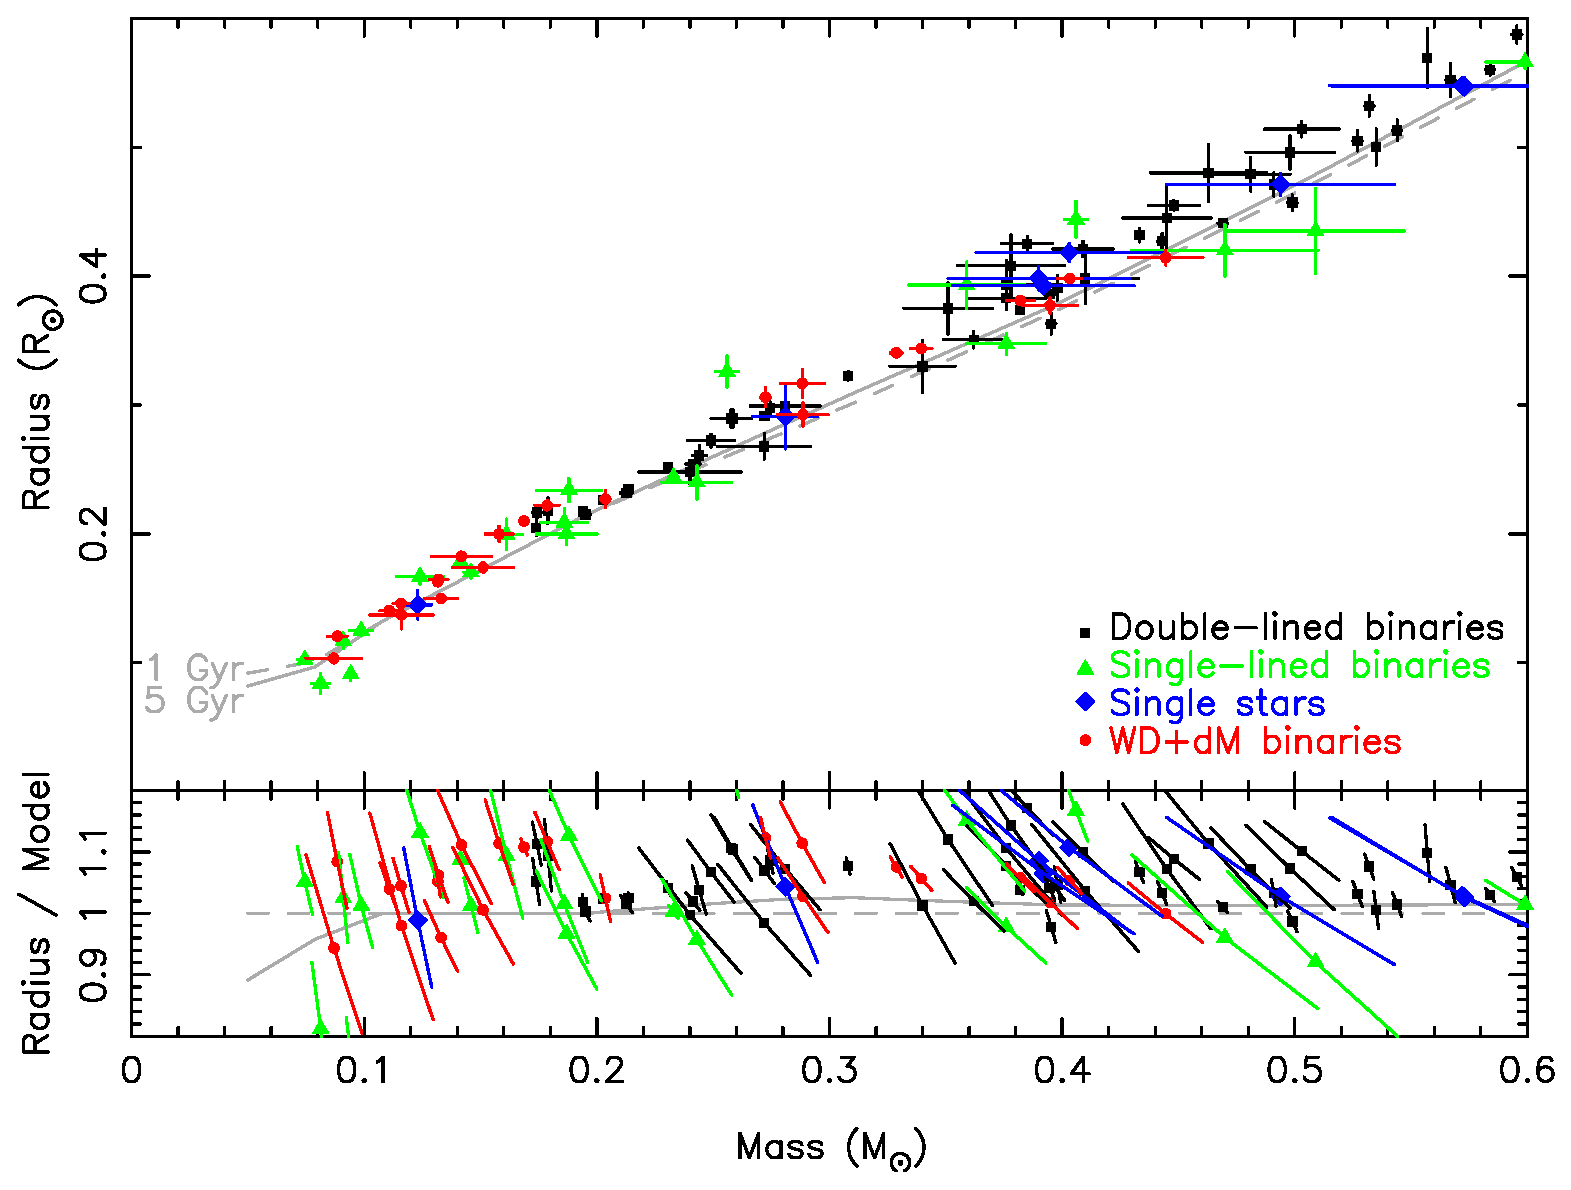
\includegraphics[width=\textwidth]{3-images/MDMR.eps}
    \caption{Mass-radius plot for low-mass stars (with mass and radius uncertainties of less than 10 per cent). The type of system that the measurement came from is indicated by the different colours and symbols and all are detailed in either Table 2 (red points) or the Appendix (all other points) of \protect\citet{2018MNRAS.481.1083P}. Also shown are the theoretical mass-radius tracks from \protect\citet{2003IAUS..211...41B}; \protect\citet{2015A&A...577A..42B}. Image taken from \protect\citet{2018MNRAS.481.1083P}}.
    \label{introduction:fig:parsons}
\end{figure}


There is an emerging tension between measurements of mass, radius and temperature compared to what is predicted from evolutionary models. M-dwarfs across the spectral type are reported to have a radius 5\% higher than expected (\citealt{2000ApJ...542..464C}; \citealt{2002ApJ...567.1140T}; \citealt{2003A&A...398..239R}; \citealt{2005ApJ...631.1120L}; \citealt{2008MmSAI..79..562R}; \citealt{2014ApJ...797...31T}; \citealt{2015A&A...577A..42B}; \citealt{2017ApJ...844..134L}). Some also have temperature hotter than predicted (\citealt{2012MNRAS.423L...1O}, \citealt{2014A&A...572A..50G}). The most glaring discrepancies are measured for low-mass stars near the convective transition ($\sim 0.35$M$_\odot$; \citealt{2007ApJ...660..732L}). The disparity also seems to be equally evident in single M-dwarfs and those in eclipsing binaries (Fig. \ref{introduction:fig:parsons}; \citealt{2013ApJ...776...87S}). A recent discovery of an over-luminous late-type M-dwarf around a solar-like star, CWW 89Ab ($\sim 0.035 M_\odot$; \citealt{2018AJ....156..168B}) suggests that this problem could extend into the brown-dwarf region. There are a few competitive theories circulated in the literature to explain the origins of this phenomena.

\subsection{Magnetic activity}

\begin{figure}
    \centering
    \includegraphics[width=\textwidth]{3-images/spada.png}
    \caption{Radius discrepancy as a function of activity indicator in a sample of low-mass stars (below solar) measured by interferometry. Image taken from \protect\citet{2013ApJ...776...87S}.}
    \label{fig:inflation_VS_Lx}
\end{figure}

The presence of magnetic fields is often invoked to explain the systematic inflation of M-dwarfs. Enhanced magnetic fields generated by the dynamo affect the convectional stability criteria leading to larger radii for the same temperature (or vice versa; \citealt{2013ApJ...776...87S}). For low-mass stars, strong surface magnetic fields (0.01-1\,kG; see \citealt{2012LRSP....9....1R}) are generated in the convective zone via dynamo mechanisms (\citealt{2013SAAS...39..187C}; \citealt{2001ApJ...559..353M}). In eclipsing binary systems, low-mass stars can be coerced into a regime of fast rotation which enhances dynamo mechanisms leading to increased magnetic activity. Stabilisation of convection in stellar models can reproduce the observed radius inflation of fully-convective M-dwarfs with reasonable surface magnetic fields, but require super-MG magnetic fields in the interior \citep{2014ApJ...789...53F}. As noted by \citet{2014ApJ...789...53F}, the presence of such a strong internal magnetic fields is unlikely for a number of reasons: turbulent dynamos in convective regimes cannot generate magnetic fields in excess of 50\,kG (\citealt{2006ApJ...638..336D}, \citealt{2008ApJ...676.1262B}) and there is no mechanism describing how MG magnetic fields would accumulate in the interior of convective stars. 
        
\citet{2005ApJ...631.1120L} conjectured that spots may explain the enhanced radius measured for GU Bootis. Star spots are manifestations of suppressed surface convection brought upon by magnetic fields. They have the effect of creating regions of different temperatures on the stellar surface; they can shift stars bluer or redder depending on there density, location, temperature differences and the photometric colours used \citep{2013ApJ...779..183F}. Significant spot coverage has the effect of lowering the overall photospheric temperature. To maintain radiative equilibrium, a star must increase its radius to conserve total flux output.  If this were to be the case, we would see a clear trend of inflation with magnetic indicators (e.g. H$\alpha$ emission, X-ray emission), rotation and age. Work by \citet{2013ApJ...776...87S} found activity indicators were independent of inflation for single and binary M-dwarfs (see Fig. \ref{fig:inflation_VS_Lx}). Significant inflation has been observed for both short period (e.g., KOI-126, $P_{\rm orb} = 1.77$\,d; \citealt{2011Sci...331..562C}) and long period systems (e.g., Kepler-16, $P_{\rm orb} = 41.1$\,d; \citealt{2011Sci...333.1602D}; \citealt{2011ApJ...737L..18W}) making it unclear whether tidally-induced magnetic fields can be blamed. 
        

\subsection{Metalicity}

\begin{figure}
    \centering
    \includegraphics[scale=0.5]{3-images/berger.png}
    \caption{Fractional deviation between the radii measured through long baseline optical interferometry and from the model predictions for stellar radius from \protect\citet{1997A&A...327.1039C} plotted as a function of metalicity. Measurements include long-baseline interferometry (filled symbols) and spectrophotometry of eclipsing binaries (open circles). The interferometry data included are from this paper (circles), PTI (\protect\citealt{2001ApJ...551L..81L}, triangles), and VLTI (\protect\citealt{2003A&A...397L...5S}, squares). The representative errors are $\pm0.2$ dex in [Fe/H] and $\pm0.1$ in fractional deviation of the radius (due to 10\% errors in the mass estimates). Image take from \protect\citet{2006ApJ...644..475B}.}
    \label{fig:berger_inflation}
\end{figure}


\begin{figure}
    \centering
    \includegraphics[scale=0.5]{3-images/Demory.png}
    \caption{Fractional deviation of single stars radii derived by interferometry  \protect\citep{1998A&A...337..403B} vs. stellar metallicity. Image take from \protect\citet{2009A&A...505..205D}.}
    \label{fig:demory_inflation}
\end{figure}

\citet{2006ApJ...644..475B} used the CHARA array to measure the radius M-dwarfs using interferometry. In their figure 5 (Fig. \ref{fig:berger_inflation}) there exists a clear trend between a stars metalicity and fractional radius residual, with less inflation observed for metal-poor stars. The same conclusion is found by \citet{2000ApJ...535..965L} and \citet{2007ApJ...660..732L} who used spectral fits to determine a systematic inflation in stars with higher metalicity. 
%Metalicity is closely related to stellar opacity and structure, and missing opacity, such as TiO, would explain an underestimation of radii for some M-dwarfs. 
However, more recent results from \citet{2009A&A...505..205D} which excluded measurements from  \citet{2006ApJ...644..475B} no longer show this trend (Fig. \ref{fig:demory_inflation}). It is likely that metallicity plays some role in inflation due to its direct affect on stellar structure. The accuracy and uncertainty of spectroscopic techniques is often questioned in \textit{hare-and-hounds} experiments which reveals significant discrepancies in stellar atmospheric parameters from identical spectra \citep{Jofre2016}. 

    
    
    
    
    



























% should be around 3 pages

%%%%%%%%%%%%%%%%%%%%%%%%%%%%%%%%%%%%%%%%%%%%%%%%%%%%%%
% Section 1. 

% P1
% - M-dwarfs are becoming popular exoplanet hosts
% - High probability of habitable zone transit

% P2
% - Number of M-dwarf exoplanets
% - Popular exoplanets

% P3
% - M-dwarf exoplanet atmospheric chemistry
% - Key chemicals
% - Influence from host on e
%%%%%%%%%%%%%%%%%%%%%%%%%%%%%%%%%%%%%%%%%%%%%%%%%%%%%%











%M-dwarfs are promising targets for exoplanet surveys. At a given distance, $a$, from a star of radius $R_\star$, an exoplanet (of radius $R_p$) is less likely to transit an M-dwarf than a K-/F-dwarf as the transit probability scales as ∼ $R_\star /a$. Conversely, we find that exoplanets in habitable zones are more likely to transit an M-dwarf than a larger star due to $a$ decreasing faster than $R_\star$ as we consider less massive stars. The transit depth of an eclipse scales as $(R_p/R_\star)^2$ so a similar planet will produce a deeper eclipse for a lower-mass star. An M-dwarf's low luminosity results in a habitable zone which is much closer to the sun than solar-type stars. If finding exoplanets in the M-dwarf habitable zone is the goal, then there is an increased geometric probability of observing a transit as well as number of transits observed in a given time period \citep{2008PASP..120..317N}. 

%Over the past decades there has been major progress in finding exoplanets around M-dwarfs. Over 200 planets have been found around M-dwarfs (\citealt{2013A&A...551A..48A}, \citealt{2014Sci...344..277Q}, \citealt{2014ApJ...784...45R}, \citealt{2015ApJ...800...99T}, \citealt{2015ApJ...804...10C}, \citealt{2015ApJ...809....7B}, \citealt{2016ApJ...818...87S}, \citealt{2016Natur.536..437A}, \citealt{2017Natur.542..456G}). These discoveries come from radial velocity surveys, transit surveys (both ground- and space-based) along with microlensing. Of note are the discoveries of exoplanets around Trappist-1 \citep{2017Natur.542..456G} and Proxima Centauri \citep{2016Natur.536..437A} which has increased the popularity of M-dwarfs for the public and scientists alike. 

%There have been recent advances in theoretical research along with observational evidence to support the conclusion that a myriad of other factors may disrupt the traditional idea of M-dwarf habitability (instead of just a function of $a$). The intense stellar activity of an early-life M-dwarf can lead to significant alterations in atmospheric chemistry \citep{2016PhR...663....1S}. In particular, the abundances of ozone \citep{2010AsBio..10..751S}, surface water,  molecular oxygen \citep{2015AsBio..15..119L} and CO$_2$ \citep{2015ApJ...806..249G} can be modified by stellar activity. In cases where close-in planets form with thick H$_2$ envelopes, however, stellar activity could photoevaporate these envelopes unveiling habitable cores \citep{2015AsBio..15..119L}.  M-dwarf emission is stronger in the IR and near-IR and so gases that absorb there are expected to have an important contribution to the discussion of habitability. Molecules like CO$_2$, H$_2$O, CHG$_4$ and O$_3$ are able to absorb a larger fraction of flux from an M-dwarf compared to the same planet around a hotter star. Planets with dense CO$_2$ atmospheres could see an increase in surface habitability through increased surface temperature \citep{2011mamo.conf..447W}. However, at the distant end of the habitable zone the effects of Rayleigh scattering will supersede atmospheric warming by CO$_2$ leading to frozen surface conditions \citep{2016PhR...663....1S}.


%%%%%%%%%%%%%%%%%%%%%%%%%%%%%%%%%%%%%%%%%%%%%%%%%%%%%%
% Section 2. 

% P1
% - Discussion of exoplanets is limited to how well we know the host
% - know thy planet
% - We cannot accurately infer parameters about the planet since we do not 
%   fully understand.
% - Turn to empirical relations

% P2
% - Attempts to measure the mass-radius plane
% - DEBs, SEB, interfereometry, WD+M, EBLMs (discussed in Sect. X)

% P3 
% - Results from Mass radius diagram
% - inflated radii
% - Hotter than expected
% - what it means for exoplanets? 
%%%%%%%%%%%%%%%%%%%%%%%%%%%%%%%%%%%%%%%%%%%%%%%%%%%%%%


%%%%%%%%%%%%%%%%%%%%%%%%%%%%%%%%%%%%%%%%%%%%%%%%%%%%%%
% Section 2. 

% P1 
% - Motivation for the first part
% - Determine robust atmospheric parameters for FGK stars 
% - SNR usually low (<20) for CORALIE optimised for RV
% - Long term systematic trends and noise make it difficult to fit lines of measure EW

% P2 
% - Use wavelet decomposition
% - capable of discering spectral features from noise/trends
% - a fast way to estimate atmospheric parameters from spectra 

% P3
% - The second part stems for the first
% - We could measure atmospheric parameters of EBLM systems identified with WASP with spectra measured from the EBLM project
% - RVs of sufficient quality
% - oppertunity to obtain follow-up photmetry
% - Measure absolute parameters of EBLMs from the ground

% P4
% - Four EBLMs were observed with K2
% - High quality lightcurves with spotted features
% - provides an oppertunity to study EBLMs in a new way with analytical lightcurves and red-noise models
% - 
% P5
% - Lots of EBLMs which have been homogenusly studied
% - Chance to study trends emerging which point to tidal inflation
% - explore possible uncertainties from assumptions of evolutionary models and orbital fit. % - What needs to be done
% - Develop EBLM studies
%%%%%%%%%%%%%%%%%%%%%%%%%%%%%%%%%%%%%%%%%%%%%%%%%%%%%%












\iffalse
Am of this thesis:
        establishe techniqe and practabitlity of mass, radii from EBBLMs
        Towards space-based photometry
        measure the Fe to get stars which arent solar
         Target the best ones for follow-up WASP
        Bottleneck with followup
                K2 and TESS will investigate

        What needs to be done

        What techniques, can we develop them? o[timising TESS/K2 CHEOPS

        How many will we need? How precisely? 1000 at 10% or 20 at 1% 
                What is the best tactic to work out a useful relation?


towards ends, have section - aims of this thesis
        Short paragraph
        aims are to develope techniqyes to study EBLMs - apply them
        Work out a strategy for EBLM studies
                Few or many? how many? 

\fi


\iffalse
\section{Properties of M-dwarfs}

 M-dwarfs form like any other star; a cloud of gas and dust clumps together by means of gravity and begins rotating. A potential source of energy comes from the gravitational potential released when such contraction occurs in the pre-main sequence (PMS). The virial theorem informs us that only half of the change in gravitational energy is available to be radiated away upon contraction; the rest heats the internal gas. It is possible to calculate\footnote{https://www.ast.cam.ac.uk/~pettini/STARS/Lecture07.pdf} the energy released assuming a radial density distribution,
%
\begin{equation}\label{virial_energy}
    \Delta E_g = \frac{3}{10} \frac{G M_\star^2}{R_\star},
\end{equation}
%
where $M_\star$ is the mass of the star, $R_\star$ is the radius and $G$ is the gravitational constant. For the Sun, $\Delta E_g \approx 1.2 \times 10^{48}$\, erg (1\,erg = $10^{-7}$\,J). If a star radiates at a luminosity $L_\star$, the \textit{Kelvin-Helmholtz timescale} timescale can be calculated,
%
\begin{equation}\label{kelvin_helmholtz_timescale}
    \tau_{\rm KH} = \frac{\Delta E_g}{L_\star}.
\end{equation}
%
This is essentially the time taken for a protostar to reach the zero-age main-sequence (ZAMS). Contraction is slowest when both $R_\star$ and $L_\star$ are small ($\tau_{\rm KH} = \Delta E_g / L_\star$ and $\Delta E_g \propto 1/R_\star$) and thus the PMS lifetime of an M-dwarf is largely spent in the final stages of contraction. For example, a 0.35\,$M_\odot$ M-dwarf remains in the PMS phase for approximately 0.18\,Gyr.\footnote{Estimated using MESA evolutionary tracks (\citealt{2016ApJS..222....8D},\citealt{2016ApJ...823..102C}) for a M-dwarf with $M = 0.3$\,$M_\odot$ at solar metalicity.} In the Solar case $\tau_{\rm KH} \sim  10^{7}$\,yr, which is two orders of magnitude smaller than the age of the solar system measured measured from radioactive dating (e.g. \citealt{2005Natur.436.1127B}).



Kelvin-Helmholtz contraction and late-stage accretion increase the young M-dwarf's angular momentum. However, interactions with the protostellar disk counteract this and reduce the M-dwarfs angular momentum \citep{2005ApJ...632L.135M}.  Eventually, the protostellar  disk is cleared and the M-dwarf enters the main sequence (MS) where few drastic changes will occur. During this phase subsequent spin-down is caused by magnetised winds carrying away angular momentum \citep{2003ApJ...586..464B}. For FGK dwarfs older than 500\,Myr, the loss of angular momentum is predictable ($\propto t^{-0.5}$) leading to the field of \textit{gyrochronolgy}: predicting a stars age from its rotation rate \citep{2008ApJ...687.1264M}. Using gyrochronology for M-dwarfs is not so straightforward. Below the convective limit there appears to be two distinct populations of faster and slower rotators ($P_{\rm rot} < 10$\,d and $P_{\rm rot} > 70$\,d; \citealt{2011ApJ...727...56I}, \citealt{2016ApJ...821...93N}) making it difficult to determine the age of field M-dwarfs. This gap likely originates from a short and rapid loss of angular momentum \citep{2011ApJ...727...56I}. M-dwarfs ultimately reach a rotational period of $> 100$\,d at a typical age of 5\,Gyr \citep{2016ApJ...821...93N}. A further indicator of age comes from H$\alpha$ emission with coincidental X-ray emission in M-dwarfs \citep{2007AJ....134.2398C}. These indicators mark the presence and strength of magnetic fields which are intertwined with age and rotation (\citealt{2006AJ....132.2507W}, \citealt{2008AJ....135..785W}).

% Other observable signatures of activity mark the evolution of M dwarfs. The presence of Hα in emission (often coincident with X-rays in emission (Reid et al., 1995; Covey et al., 2007)) signals the presence and strength of magnetic activity and decreases with age (West et al., 2006, 2008). Across the M spectral class, the “active" duration of a star’s life varies from 1 Gyr in the case of M0 dwarfs to 8 Gyr or more for spectral type M8 (West et al., 2006).

% continue using https://arxiv.org/pdf/1610.05765.pdf

A scaling argument used by \citet{2016PhR...663....1S} states that a star's main-sequence lifetime scales as $M_\star / L_\star$, where $L_\star \sim M_\star^3$ for low-mass stars \citep{2009itss.book.....P}. A 0.1-$M_\sun$ star is therefore expected to stay on the main sequence 100 times longer compared to the Sun. In reality however, this factor is more like 1000 due to added sources of longevity unique to M-dwarfs. The first is slower rate of fusion as a consequence of a cooler core temperature. The second stems from the convective nature of M-dwarfs. This replenishes hydrogen in the core which is being fused via the P-P chain whilst simultaneously preventing He ash building up. M-dwarfs therefore have access to almost all of their hydrogen to burn \citep{2004RMxAC..22...46A} compared to Solar type stars which are restricted to hydrogen in the core (about 10\%; \citealt{2016PhR...663....1S}). The combined effect extends the MS lifetime of M-dwarfs well in excess of Hubble time ($\sim 200$\,Gyr; \citealt{1998A&A...337..403B}).
\fi


\iffalse
\section{Initial mass function}

Measuring the properties of many individual stars (e.g. from clusters) reveal their evolutionary state, age and mass. The distribution of stellar masses at birth is known as the initial mass function (IMF). The IMF has been subjected to numerous reviews (\citealt{2010ARA&A..48..339B}; \citealt{2012EAS....57...45J}; \citealt{2013pss5.book..115K}; \citealt{2014prpl.conf...53O}; \citealt{2017ApJ...841...68V}). One of the first attempts to measure the IMF determined a power-law function which decreases between 0.1-10\,$M_\odot$. However, recent studies (\citealt{2000ApJ...544.1044L};
\citealt{2000ApJ...540.1016L}; 
\citealt{2014prpl.conf...53O};
\citealt{2003PASP..115..763C};
\citealt{2006ApJ...640L..63L}) have found a break from the power law in the mass range 0.05-10\,$M_\odot$ (Fig. \ref{fig:IMF_late_stars}). 

% see 6.2 from https://arxiv.org/pdf/1402.0867.pdf
% Theories for the origin of the peak of the IMF can be divided into two groups based on what additional piece of physics they choose to add to assign a definite mass scale

There are three possible explanations which could explain this peak this peak. The first is the \textit{Jeans mass hypothesis} which states that the peak of the IMF is a reflection of the mean-density in star-forming clouds (\citealt{1992MNRAS.256..641L}, \citealt{2005MNRAS.356.1201B}) and has been applied to cosmological models (\citealt{2007ApJ...668..667T}, \citealt{2012MNRAS.423.3601N}). A serious shortcoming of this approach is the choice of scale; what should be counted as the \textit{cloud}? In simulations by \citet{2007ApJ...668..667T} and  \citet{2012MNRAS.423.3601N}, the initial speed of sound and density (which describe the Jeans mass) are entered manually, but the latter choice depends which material is traced (i.e. low-density tracer like CO or a higher one). The second potential origin invokes \textit{deviations from isothermality}. Isothermality holds only approximately for molecular clouds and such deviations may be important for setting the characteristic mass of stars (\citealt{2001BpJ....81.2020G},\citealt{2007PASJ...59..589O},\citealt{2013A&A...557A..90V}). The third mechanism involves invoking \textit{non-ideal MHD processes}. However one of the most probable process, ambipolar diffusion (the diffusion of positive and negative species due to interaction with an electric field) is not mass dependent providing the ionization fraction behaves as a power-law function of density \citep{2010ApJ...709..308M}.

Many space missions probe the IMF for the lowest-mass stars: the Spitzer space telescope \citep{2004ApJS..154....1W}, the Herschel space observatory \citep{2010A&A...518L...1P} and the wide-field infrared survey explorer (WISE; \citealt{2010AJ....140.1868W}). 
%The James Webb space telescope \citep{2006SSRv..123..485G} will further contribute to the bottom-end of the IMF.
Complimenting these are a selection of ground-based surveys which are magnitude-limited: the Two Micron All Sky Survey \citep{2006AJ....131.1163S}, the Sloan Digital Sky Survey (SDSS; \citealt{2000AJ....120.1579Y}) and the Visible and Infrared Survey Telescope for Astronomy (VISTA; \citealt{2001ASPC..232..339E}). An important conclusion from decades of probing the IMF is that low-mass stars ($\leq 0.6\,M_\sun$)form 70\% of the total stellar systems within a distance of 10\,pc \citep{2006AJ....132.2360H}.  


\begin{figure}
    \centering
    \includegraphics{3-images/IMF.png}
    \caption{The IMF $\xi(\log m) = dn/d\log m$ of stars in the Orion Nebula Cluster as inferred from \textit{Hubble Space Telescope} photometry. In each panel the black points show the data; the error bars are the 1$\sigma$ errors that result from a combination of counting statistics and incompleteness. Although the underlying data in each panel are the same, the three panels show the results of converting the observed colours and magnitudes to stellar masses using three different models. The bottom panel uses the models of \citet{1998ASPC..134..442D}, while the top two panels both use the models of \citet{1998A&A...337..403B}, using two different methods for handling stars that fall outside Baraffe et al.'s model grid. The red solid and dashed lines are the single-star and system IMFs of \citet{2003PASP..115..763C}, while the black curve is the best fit of the data to a lognormal functional form; the yellow band shows the $1\sigma$ uncertainty on the fit. Taken from  \citet{2012ApJ...748...14D}. }
    \label{fig:IMF_late_stars}
\end{figure}


\fi


%\section{The M spectral type}\label{spec_analysis_M_dwarf}

% sect. 2.1 from https://arxiv.org/pdf/1610.05765.pdf
% sect. 2.3 from https://arxiv.org/pdf/1610.05765.pdf

%The spectral type of an M-dwarf is generally estimated by comparing its spectrum to a set of benchmark spectra (e.g. \citealt{2007AJ....134.2398C}). The spectral type M is defined by strong moleculer absorption from titanium oxide (TiO) blueward of the optical ($\sim$450-570\,nm; \citealt{morgan}). Molecular opacity from diatomic hydrogen (H$_2$), water (H$_2$O) and vanadium oxide (VO) obscure the continuum making the task of determining atmospheric parameters a subtle endeavour (see Fig. \ref{fig:M6_spectra}). The classification of M-dwarf boundaries is subject to the quirks of astronomical history. For example, strong TiO lines can be measured at redder wavelengths for stars hotter than M0 but required the development of red-sensitive detectors at the end of 20$^{th}$ century (\citealt{1991ApJS...77..417K}, \citealt{1991AJ....101..662B}). 

%The lower limit of the M spectral type is M7/M8 (the hydrogen burning limit; \citealt{1998A&A...337..403B}). Determining spectral types for stars in this regime is challenging as small mass and metalicity variations result in physical variations capable of moving objects from one category to another \citep{2014AJ....147...94D}. Young brown dwarfs look almost identical to late M-dwarfs and requires diligent analysis of the atmosphere to discern the two. For example, molecules like ammonia or methane can only survive at colder temperatures ($\sim 1000$\,K; \citealt{1999A&A...349L..41C}) pointing towards a brown-dwarf. Brown dwarfs are also distinguished by their inability to fuse hydrogen, but they can fuse less abundant isotopes like deuterium and lithium. A further complication arises from spectral types as late as L2 occasionally possessing the minimum mass required for hydrogen fusion to occur \citep{2014AJ....147...94D}. 

%\begin{figure}
 %   \centering
 %   \includegraphics[scale=0.5]{3-images/M_dwarf_spectra.png}
%    \caption{Illustrative example of spectra for an inactive M1 %star and an active M6 star with strong molecular and atomic %feautures labelled. Taken from %\protect\citet{2007AJ....133..531B}.}
%    \label{fig:M6_spectra}
%\end{figure}


%\begin{figure}
 %   \centering
%    \includegraphics{3-images/CaH2_fig_2_PASP_118_840_218.jpg}
%    \caption{Temperature vs. CaH2 index for program stars from \protect\citealt{2006PASP..118..218W}. The line is a least‐squares fit: Teff = (2696 + 1618 × CaH2) K. Image taken from Fig.2 of \protect\citealt{2006PASP..118..218W}.}
%    \label{fig:CaH2_index}
%\end{figure}

%Currently there are no robust ways of measuring metalicity from low-resolution spectra of M dwarfs \citep{2008AJ....135..785W}. It is possible to use calibrated molecular indices to measure an M-dwarf metalicity using measurements of equivalent widths from atomic lines in high-resolution spectra ($\lambda / \Delta \lambda \approx 33,000$; \citealt{2008AJ....135..785W},\citealt{2007AJ....134..778M}). Despite their abundance in the Galaxy, their faintness thwarts obtaining high resolution spectra of more distant M-dwarfs and thus an alternate method is required. Low resolution spectra ($R \approx 3000$) can go approximately 3 mag. fainter ($V \geq 16$ for a 4-m class telescope) and permits the measurements of molecular indices. Two such are the CaH2 and TiO5 indices which measure CaH and TiO band strengths respectively. CaH2 is strongly correlated with photospheric temperature (see Fig. \ref{fig:CaH2_index}). TiO5 depends on temperature and metalicity: for a given temperature or CaH2 value, a smaller TiO5 value indicates a smaller metallicity. Measuring $\log g$ can be done using the unblended FeH lines in the infrared with careful treatment micro-/macro-turbulence \citep{2009AIPC.1094..816W}. The alkali lines also show large wing variations due to pressure broadening. The K- and Na-line pairs (768\,nm and 819\,nm, respectively) are particularly sensitive to both $\log g$ and [Fe/H] (Fig. 2 of \citealt{2016A&A...587A..19P}). However, these lines are contaminated from O$_2$ and H$_2$O from the earths atmosphere. % Significant disagreement ($> 3\sigma$) between alkali-line metalicity and photometric/spectroscopic metalicity has been noted. 
    









\section{Empirical relations of M-dwarfs}\label{intro:empirical}
% summary of the current laws
% https://arxiv.org/pdf/1501.01635.pdf
% - Sect 8.4
% - Delfosse et al. (2000) vs. of the mass inferred from the models (Section 8.3).

Measurements of absolute stellar parameters for low-mass stars can be used to derive empirical relations to bypass the disagreement with stellar models. Such relations join observable parameters with absolute parameters (e.g. luminosity-mass relations), or only absolute parameters (e.g. mass-radius relations). In principle, these are applicable to more distant and fainter stars from which they are calibrated \citep{2013AJ....145...52M}. In the sample presented by \citet{2010MNRAS.402.2591P} (Fig. \ref{introduction:fig:parsons}), there are few single stars (measured with interferometry) with mass below $\sim 0.4\,M_\odot$; empirical calibrations calibrated from this sub-sample will only be accurate for the early-type M-dwarfs. The situation is somewhat better for double-lined eclipsing binaries; these are abundant across the M-dwarf spectral type down to $\sim 0.2\,M_\odot$. Perhaps the best choice is single-lined eclipsing binaries. The sample presented by \citet{2010MNRAS.402.2591P} are abundant across the entire spectral type but have precision in mass and radius inferior to double-lined eclipsing binaries and single stars. It is imperative to  exercise caution when constructing empirical relations to ensure that they come from a sample of homogeneously measured systems and the extent of such calibrations are explicitly stated.  
%Precise absolute parameters for M dwarfs can be used to construct empirical relations between observable and absolute parameters which are, in principle, applicable to more distant and fainter stars \citep{2013AJ....145...52M}.
%Such relations are advantages as there is no dependency on stellar models which have been shown systematically underestimate the radius and temperature of M-dwarfs.

%   - Importants to consider for empirical
%   - This is highlighted in the recently collations of M-dwarfs with masses and radius uncertainties known to better than 10 % (Parsons, Fig x)
%   - there are few interferometric samples below  0.4 M_sol 
%   - Therefroe empirical calibrations are only good for early type M-dwarfs
%   - The problem is somehat better with double-lined binary stars, althought the sample presented by Parsons has no calibrators below 0.17 M_sol meaning that they are unsuitable for the latest M-dwarfs
%   - Single-lined eclipsing binaries are better suited to this task. They cover the whole spectrl type





\subsection{Luminosity relations}\label{introduction:luminosity_relations}


The mass of an M-dwarf is a fundamental property from which most other stellar properties depend steeply on. Therefore a mass-luminosity relation is a useful astrophysical tool which can convert observable light into a stellar mass and derive interstellar mass functions from more readily obtained luminosity functions. The interstellar mass function has been subjected to numerous reviews (\citealt{2010ARA&A..48..339B}; \citealt{2012EAS....57...45J}; \citealt{2013pss5.book..115K}; \citealt{2014prpl.conf...53O}; \citealt{2017ApJ...841...68V}). One of the first attempts to measure the IMF determined a power-law function which decreases between 0.1-10\,$M_\odot$. However, recent studies (\citealt{2000ApJ...544.1044L};  \citealt{2000ApJ...540.1016L};  \citealt{2014prpl.conf...53O}; \citealt{2003PASP..115..763C}; \citealt{2006ApJ...640L..63L}) have found a break from the power law in the mass range 0.05-10\,$M_\odot$. Numerous theories have been put forward to explain the deviation (e.g. \citealt{1992MNRAS.256..641L}; \citealt{2005MNRAS.356.1201B}; \citealt{2012MNRAS.423.3601N}; \citealt{2001BpJ....81.2020G}; \citealt{2007PASJ...59..589O}; \citealt{2013A&A...557A..90V}; \citealt{2010ApJ...709..308M}); each has its own degree of successes and shortcomings which is beyond the scope of this work. However, the field will be better understood with accurate empirical relationships between fundamental stellar properties. 

The mass-luminosity relationship is well constrained for solar-type and intermediate stars. This is in-part due to the large number of systems which have mass measurements better than 1\% uncertainty \citep{1991A&ARv...3...91A} and typically match stellar models when both metallicity and evolution is accounted for \citep{1997IAUS..189.....B}. This work addresses empirical relations of M-dwarfs ($M \lesssim 0.6\, M_\odot$) where stellar models face two major hurdles:
%
\begin{itemize}
    \item the onset of low temperature electron degeneracy in the stellar core  \citep{2000ApJ...542..464C};
    \item a complex cold and high gravity stellar atmosphere, dominated by molecular and dust opacity \citep{1998ASPC..134..370A}.
\end{itemize}
%
There has been considerable progress in stellar models over the last few decades which has addressed shortcomings such as boundary conditions of stellar interior equations and atmospheric models  (e.g. \citealt{2016ApJ...823..102C}; \citealt{2007A&A...472L..17C}). However, the description of input physics still remains incomplete: some molecular opacities and line-lists remain unfinished and the validity of the mixing-length approximation remains questionable. Therefore an independent check of absolute parameters with a mass-luminosity relationships is desirable.


\citet{2000A&A...364..217D} used a sample of 32 M-dwarfs in eclipsing and astrometric binaries to derive empirical mass-luminosity relations. They adopted a 10\% mass accuracy cutoff for the inclusion as a compromise between good statistics and quality of individual measurements. Absolute magnitudes for various colours ($M$) were then calibrated against mass using fourth-degree polynomials:
%
%\begin{displaymath}
%\begin{array}{l}

\begin{eqnarray}
\log(M/{M_\odot}) &=& 10^{-3}{\times}[0.3+1.87{\times}{M_V} +7.6140{\times}{M_V}^2 \nonumber \\
&-&1.6980{\times}{M_V}^3 + 0.060958{\times}{M_V}^4] {\ \ \ \ \  \ \ \  \ \ \ \ }{\mathrm{for}} {\ }{M_V}  \in [9,17]
\end{eqnarray}

\begin{eqnarray}
\log(M/{M_\odot}) &=&10^{-3}{\times}[1.6+6.01{\times}{M_J}
+14.888{\times}{M_J}^2  \nonumber \\
&-&5.3557{\times}{M_J}^3 +2.8518.10^{-4}{\times}{M_J}^4] {\ \ \  \ \ \ \ \ \  \ \ }{\mathrm{for}} {\ }{M_J} \in [5.5,11] 
\end{eqnarray}

\begin{eqnarray}
\log(M/{M_\odot}) &=&10^{-3}{\times}[1.4+4.76{\times}{M_H}
+10.641{\times}{M_H}^2 \nonumber \\
 &-&5.0320{\times}{M_H}^3 +0.28396{\times}{M_H}^4] {\ \ \ \ \ \ \ \ \ \ \ \ \ \ \ \ }{\mathrm{for}} {\ }{M_H} \in [5,10] 
\end{eqnarray}

\begin{eqnarray}
\log(M/{M_\odot}) &=&10^{-3}{\times}[1.8+6.12{\times}{ M_K} +13.205{\times}{ M_K}^2 \nonumber \\
 &-&6.2315{\times}{ M_K}^3+0.37529{\times}{ M_K}^4
{\ \ \ \ \ \ \ \ \ \ \ \ \ \ \ \ \ \ \ }{\mathrm{for}} {\ }{ M_K} \in [4.5,9.5] 
\end{eqnarray}

\begin{eqnarray}
\log(M/{M_\odot})  &=&10^{-3}{\times}[7.4+17.61{\times}{ (V-K)} \nonumber  \\
&+&33.216{\times}{ (V-K)}^2 +34.222{\times}{ (V-K)}^3 \nonumber  \\
&-&27.1986{\times}{ (V-K)}^4 +4.94647{\times}{ (V-K)}^5  \nonumber \\
&-&0.27454{\times}{ (V-K)}^6 {\ \ \ \ \ \ \ \ \ \ \ \ \ \ \ \ \ \ \ \ \ \ \ \ \ \ \ \ \ \ \ \ \ \ }{\mathrm{for}} {\ }{ V-K} \in [4,7] 
\end{eqnarray}
%
These relations are impressively accurate for the JHK magnitudes and relatively poorer for $M_V$ due to the increasing effect of metallicity on the M-dwarfs spectra blue of the infrared \citep{2003IAUS..211..413S}. This sample has measurements of mass spanning the entire spectral type with most residing in the 0.1-0.4\,$M_\odot$ range. In practise, mass-luminosity relation of \citet{2000A&A...364..217D} is typically used with assumed 10\% error (e.g. \citealt{2015ApJ...804...64M}). 


\begin{figure}
    \centering
    \includegraphics[width=\textwidth]{3-images/f7.pdf}
    \caption{Top: $R_*$ as a function of absolute $K_S$-band magnitude. The best-fit to the data is shown as a blue dashed line. $M_{K}$ and radius both depend on the distance, so the errors are correlated. Hence we show a one-sigma error ellipse in the top-left which indicates the typical 1$\sigma$ errors for a typical point ($M_{K_S}\simeq6.6$, $R_*\simeq0.35$). Bottom: fractional radius residual to the fit. All points are colour-coded by metallicity. Image taken from \protect\citet{2015ApJ...804...64M}. }
    \label{intro:fig:Mann1}
\end{figure}


\begin{figure}
    \centering
    \includegraphics[width=\textwidth]{3-images/f10.pdf}
    \caption{Spectroscopically derived \teff\ as a function of different color combinations. The best-fit is overplotted as a blue dashed line. The bottom panels show the fit residuals. Fit coefficients are given in Table~\ref{intro:table:mann}. Image taken from \protect\citet{2015ApJ...804...64M}.}
    \label{intro:fig:Mann2}
\end{figure}

\begin{sidewaystable}[]
    \centering
    \caption{Mass and radius relations of \protect\citet{2015ApJ...804...64M}.}

    \begin{tabular}{l l | r r r r r r | r r r}
    \hline
    Y & X & a & b & c & d & e & f  & $\sigma^a$ & $\chi_\mu$ \\
    \hline
    
$R_*$ & $M_{K_S}$    & $ 1.9515$ & $-0.3520$ & $0.01680$ &  &  &  &   2.89 &    0.93\\
$R_*$ & $M_{K_S}$,[Fe/H]  & $ 1.9305$ & $-0.3466$ & $0.01647$ & &  &  $0.04458$ &   2.70 &    0.88\\
$R_*$ & $T_{\rm eff}$/3500  & $ 10.5440$ & $ -33.7546$ & $  35.1909$ & $-11.5928$\phantom{0} & \nodata & \nodata &  13.4 &    2.35\\
$R_*$ & $T_{\rm eff}$/3500,[Fe/H]  & $16.7700$ & $-54.3210$ & $57.6627$ & $-19.6994$\phantom{0} & \nodata & $  0.4565$\phantom{0} &   9.3 &    1.10\\
 \hline
 
 
 
 $T_{\rm eff}$/3500 & $BP-RP$ & $3.245$ & $-2.4309$ & $1.043$ & $-0.2127$ & $0.01649$ & & 52 & 0.88\\
$T_{\rm eff}$/3500 & $V-J$ & $2.840$ & $-1.3453$ & $0.3906$ & $-0.0546$ & $0.002913$ & &  55 & 0.93\\
$T_{\rm eff}$/3500 & $V-Ic$ & $2.455$ & $-1.5701$ & $0.6891$ & $-0.1500$ & $0.01254$ & &  53 & 0.94\\
$T_{\rm eff}$/3500 & $r-z$ & $1.547$ & $-0.7053$ & $0.3656$ & $-0.1008$ & $0.01046$ &  & 58 & 1.06\\
$T_{\rm eff}$/3500 & $r-J$ & $2.445$ & $-1.2578$ & $0.4340$ & $-0.0720$ & $0.004502$& & 58 & 1.04\\
\hline
$T_{\rm eff}$/3500 & $BP-RP$,[Fe/H] & $2.835$ & $-1.893$ & $0.7860$ & $-0.1594$ & $0.01243$ & $0.04417$ &  45 & 0.60\\
$T_{\rm eff}$/3500 & $V-J$,[Fe/H] & $2.515$ & $-1.054$ & $0.2965$ & $-0.04150$ & $0.002245$ & $0.05262$ &  42 & 0.53\\
$T_{\rm eff}$/3500 & $V-Ic$,[Fe/H] & $1.901$ & $-0.6564$ & $0.1471$ & $-0.01274$ & \nodata & $0.04697$ &  48 & 0.67\\
$T_{\rm eff}$/3500 & $r-z$,[Fe/H] & $1.572$ & $-0.7220$ & $0.3560$ & $-0.09221$ & $0.009071$ & $0.05220$ &  50 & 0.71\\
$T_{\rm eff}$/3500 & $r-J$,[Fe/H] & $2.532$ & $-1.319$ & $0.4449$ & $-0.07151$ & $0.004333$ & $0.05629$ &  47 & 0.63\\

\hline 
\hline
    \end{tabular}
    \label{intro:table:mann}
\end{sidewaystable}

Empirical radius-/temperature-luminosity calibrations have been derived from interferometric observations of single stars. \citet{2015ApJ...804...64M} used measurements of 183 nearby K7-M7 stars to derive a radius-luminosity relation using a third-order polynomial with a correction for metallicity (Fig. \ref{intro:fig:Mann1}),
%
\begin{eqnarray}
    R_\star =  \left( a + bX + cX^2 \right) \left[ \times \left( 1 + f[Fe/H] \right) \right],
\end{eqnarray}
%
where $X$ is the relevant absolute magnitude and $a$, $b$, $c$ and $f$ are coefficients summarised in Table \ref{intro:table:mann}. The best fit has a remarkably tight scatter of 2.9\% despite an average radius uncertainty of 3-4\%. There is small, but statistically significant improvement including [Fe/H], with a resulting scatter of 2.7\%. 
%This is useful for reducing systematic errors between planet size and metallicity. 
They tested calibrations for all SDSS and 2MASS magnitudes ($grizJHK_s$); $K_s$ had the lowest scatter due to the increasing shape of the spectra at bluer wavelengths due to metallicity. \citet{2015ApJ...804...64M} also created a colour-temperature relationship using a fourth-order polynomial with a metallicity correction (Fig. \ref{intro:fig:Mann2}),
%
\begin{equation}
    T_{\rm eff}/3500 = a + bX + cX^2 + dX^3 + eX^4 \left[ + f[Fe/H] \right],
\end{equation}
%
where $X$ is a metal-sensitive colour (Table \ref{intro:table:mann}). The authors caution the use of of this calibration outside the colour range of the sample where non-real slope changes are observed. However, the sample is well-populated between $\sim$2800-4000\,K and the calibration appears to have a scatter below 100\,K which significantly decreases for redder objects.  

% https://arxiv.org/pdf/1501.01635.pdf
% http://articles.adsabs.harvard.edu/cgi-bin/nph-iarticle_query?2000A%26A...364..217D&amp;data_type=PDF_HIGH&amp;whole_paper=YES&amp;type=PRINTER&amp;filetype=.pdf


\subsection{Mass-radius-temperature relations}

% include FIGURE 9 from MANN!


\begin{figure}
    \centering
    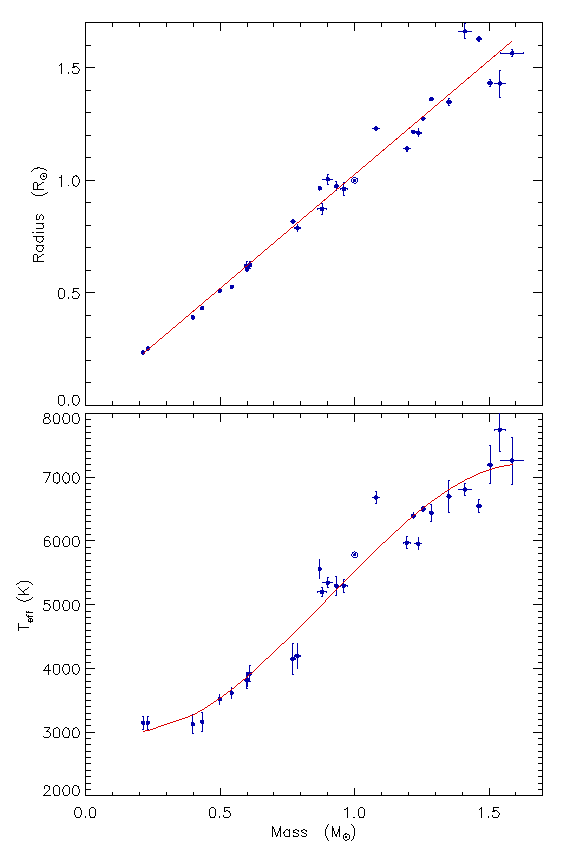
\includegraphics{3-images/final-EB.eps}
    \caption{Mass--radius and mass--$T_{\rm eff}$\ diagrams for exoplanet host stars. The filled circles show the properties of stars in eclipsing binary systems and the Sun is represented by a $\odot$. The solid lines represent the mass--radius and mass--$T_{\rm eff}$\ relations. Image take from \protect\citet{2009MNRAS.394..272S}.}
    \label{introduction:fig:TEPcalibration}
\end{figure}


Testing evolutionary models requires a diligent comparison of mass, radius and temperature measurements. Because there is a commonly observed discrepancy between between observed and predicted fundamental parameters (Sect. \ref{introduction:tension}), it is common-place to derive empirical relations instead. A rudimentary approach by \citet{2009MNRAS.394..272S} achieved this using a sample of 29 stars in eclipsing binaries (plus the Sun) which covers the masses $0.124$-$1.586\,M_\odot$  (Fig. \ref{introduction:fig:TEPcalibration}). They fitted a first-order polynomial to the mass-radius relation which did not account for [Fe/H] and age,
%
\begin{equation}
    R_\star = (0.00676 \pm 0.03408) + (1.01824 \pm 0.03368) M_\star,
\end{equation}
%
where $R_\star$ and $M_\star$ are in solar units. The authors fit has an rms scatter of 0.073\,$R_\star$ about the fit; the scatter is significantly smaller for low-mass stars ($\leq 0.6\,M_\odot$) but there are less than 10 stars with masses below 0.6\,$M_\odot$. \citet{2009MNRAS.394..272S} also present an empirical mass-temperature relationship,
%
\begin{eqnarray}
T_{\rm eff} & = & (3217 \pm 564) - (2427 \pm 2304) \cdot M_\star \nonumber\\
      &   & + (7509 \pm 2802) \cdot M_\star^2 - (2771 \pm 1030) \cdot M_\star^3,
\end{eqnarray}
%
which has an rms scatter of 328\,K about the best fit. 


\begin{figure}
    \centering
    \includegraphics[width=\textwidth]{3-images/f9.pdf}
    \caption{Top: $R_*$ as a function of stellar $T_{\rm eff}$. The derived $R_*$ depends on $T_{\rm eff}$ so the errors are strongly correlated. A typical error is shown a gray ellipse in the top left of the plot. The best-fit ignoring [Fe/H] is shown as a dashed blue line. Bottom: residual from the best-fit. Points are coloured according to their metallicity. Image taken from \protect\citet{2015ApJ...804...64M}.}
    \label{intro:fig:Mann3}
\end{figure}


\begin{figure}
    \centering
    \includegraphics[width=\textwidth]{3-images/f4.pdf}
    \caption{Mass--radius diagram for stars in our sample (red circles) and those from low-mass eclipsing binaries (LMEBs, blue stars). A typical error bar on our measurements is shown to the left. Stars in our sample are color-coded by their metallicity. The fit to both samples is shown as a dashed line. The bottom panel shows the fractional residual between these two fits. Image taken from \protect\citet{2015ApJ...804...64M}.}
    \label{intro:fig:Mann4}
\end{figure}


Interferometry can provide both radius and temperature to a high precision. In addition to the luminosity relations stated above, \citet{2015ApJ...804...64M} created an empirical radius-temperature calibration (Fig. \ref{intro:fig:Mann3}),
%
\begin{equation}
    R_\star = \left( a + bX + cX^2 \right) \times (1 + f[Fe/H])
\end{equation}
%
where $X = T_{\rm eff} / 3500$\,K (Table \ref{intro:table:mann}). This calibration has a significant scatter in radius of 13\% which is reduced to 9\% when metallicity is accounted for.  Interformetric measurements are excluded from empirical mass relations as the mass of a single star is typically determined from its colours. \citet{2015ApJ...804...64M}, who determined stellar mass through colour relations from \citet{2000A&A...364..217D}, attempted to create a \textit{semi-empirical} mass-radius relation with a second order polynomial. Their fit is compared to a sample of detached eclipsing binaries with mass and radius errors below 5\% and find a notable discrepency above 0.65\,$M_\odot$. The authors state that model-inferred masses better reproduces the mass-luminosity relation measured for low-mass eclipsing binaries and thus the disagreement in Fig. \ref{intro:fig:Mann4} is most likely due to errors in the luminosity relation of \citet{2000A&A...364..217D}, which was based on only 3 objects with masses in this range.

\begin{figure*}[!htb]
\centering
\begin{minipage}{0.47\linewidth}
\includegraphics[angle=270,scale=0.45]{3-images/stellar_mass_as_teff_metal_harps_m_gto_v26feb15.png}
\end{minipage}
\begin{minipage}{0.47\linewidth}
\includegraphics[angle=270,scale=0.45]{3-images/stellar_radii_as_teff_metal_harps_m_gto_v26feb15.png}
\end{minipage}
\caption{Stellar mass (left panel), and radius (right panel), as a function of the effective temperature. Stars are plotted using different colours and symbols according to their metallicity. Several fits for fixed metallicity values are plotted: +0.15 (dashed line), +0.00 (solid line), -0.15 (dash-dotted line), and -0.30 (dotted line). The upper left panel shows the differences between the mass and those derived by using  \protect\cite{1993AJ....106..773H} relationship. Image taken from \protect\citet{2015A&A...577A.132M}.}
\label{intro:fig:mald}
\end{figure*}

Similar relations were derived by \citet{2015A&A...577A.132M} using interferometric observations of M-dwarfs. They fitted radii with masses calculated from the mass-luminosity relations of \citet{1993AJ....106..773H} using a second-order polynomial,
%
\begin{equation}
    R = 0.0753 + 0.7009 M + 0.2356M^2.
\end{equation}
%
There are significantly more calibrators in the \citet{2015A&A...577A.132M} sample than the \citet{2009MNRAS.394..272S} and provides a much tighter fit; the rms about the best fit is 0.02\,$M_\odot$ and 0.02\,$R_\odot$. However, there sample consists of stars measured by intereferometry and those in eclipsing binary systems and there is no attempt to account for age or metallicity. However, they do form mass-temperature and radius-temperature relations using third-order polynomials which account for metallicity,
%
\begin{eqnarray}
    M_\star &=& -171.616 + 0.139 T_{\rm eff} - 3.776 \times 10^{-5} T_{\rm eff}^2 \nonumber \\
    &+&3.419 \times 10^{-9} T_{\rm eff}^3 + 0.382 \rm [Fe/H];
\end{eqnarray}
\begin{eqnarray}
    R_\star &=& -159.857 + 0.130 T_{\rm eff} - 3.534 \times 10^{-5} T_{\rm eff}^2 \nonumber \\
    &+&3.208 \times 10^{-9} T_{\rm eff}^3 + 0.347 \rm [Fe/H].
\end{eqnarray}
%
These calibrations (Fig. \ref{intro:fig:mald}) are relatively good: the scatter in mass and radius is 0.02\,$M_\odot$ (13.1\%) and 0.02\,$R_\odot$ (11.8 \%) respectively and are valid for $3340 \, \rm K < T_{\rm eff} < 3840\, \rm K$ and $-0.4 \, \rm dex < \rm [Fe/H] < +0.16\, \rm dex $. The authors caution that relative errors in mass tend to increase for low-mass stars, and can be up to 40\% for stars with mass below 0.25\,$M_\odot$. The same is true for uncertainty in radius and can be larger than 20\% for stars with radius below 0.35\,$R_\odot$. A possible explanation for the increase in mass error for later-type M-dwarfs is that the relative mass errors from the \citet{1993AJ....106..773H} relationship tend to be larger at lower masses.


\section{Eclipsing binary, low mass}\label{introduction:EBLM}
% lack of calibratable points
% solution lies with EBLMs

Measuring the absolute parameters of M-dwarfs typically involves stars which are measured by interfereometry or those in binary configurations such that the companions occult the light from one another.  For low-mass stars ($< 0.6\,M_\odot$) there is a dearth of systems with absolute parameters known to the desired precision of a few percent. A recent compilation of M-dwarfs with masses and radii known to better than 10\% yield only 90 M-dwarfs \citep{2018arXiv180505841C}. The reason is due to the intrinsic brightness of M-dwarfs and low-probability of finding eclipsing binary systems from which mass and radius can be empirically derived. While the sample presented by  \citep{2018arXiv180505841C} is sizeable, it is not large enough to reliably determine empirical relations and they are not measured using consistent and homogenous techniques.

A solution to this problem is in the remit of exoplanet surveys. The Wide Angle Search for Planets  (WASP; \citealt{2006PASP..118.1407P})  is a survey for $0.8$--$ 2 \rm \, R_{Jup}$ objects transiting solar-like stars. Objects in this radius range can have masses which span three orders of magnitude, from Saturn-like planets to M-dwarfs. Consequently, WASP photometry has been used to identify hundreds of FGK stars with transiting M dwarf companions as a by-product of its successful exoplanet search. These systems are termed EBLMs (eclipsing binary, low-mass). The EBLM consortium has invested considerable effort to characterise these systems, including hundreds of hours of telescope time to measure their spectroscopic orbits. The determination of absolute parameters of EBLM systems has been coordinated within the EBLM project. This first three instalments of the project measured the absolute parameters of 4 EBLMs: EBLM I \citep{2013A&A...549A..18T}, EBLM II \citep{2014A&A...572A..50G} and EBLM III \citep{vonBoetticher2017}. Secondary eclipses of J0113+31 (EBLM II) resulted in an effective M-dwarf temperature that is $\sim600$\,K hotter than predicted with evolutionary models. The fourth instalment (EBLM IV) was the product of hundred of hours of observations of EBLMs leading to the spectroscopic orbits of 118 EBLM systems.  


%The accumaltion of this work has lead to the absolute parameters of 4 EBLM systems as part of the EBLM project (\citealt{2013A&A...549A..18T}, \citealt{2014A&A...572A..50G}, \citealt{vonBoetticher2017}, \citealt{Triaud2017}). 

%The main aim of the EBLM project is to improve our understanding of low-mass stars using accurate mass and radius measurements for transiting companions to FGK stars.

Almost a thousand candidate EBLM systems have been flagged as a result of the WASP project.%
\footnote{As of 10$^{th}$ Oct 2018.}
%
The M dwarfs in EBLM systems are most likely to be found around F stars as oppose to G-/Kstars. The reason for this has its origins in tidal evolution theory. If the rotation of the primary star is less than that of the companion stars orbital period, then the torque induced by tidal interaction will increase the rotation of the host star. However, this is at the expense of the semi-major axis which must decrease in order to conserve angular momentum. This causes a spiral-like orbit which may eventually lead to engulfment of the low-mass companion. This is most probable for G/K host stars whereas the rotation of F-type hosts is sufficient to avoid colliding (\citealt{2017IAUS..328..308P}; \citealt{2011A&A...525A..68B}; \citealt{2011A&A...533A..83B}).

The sample presented by \citet{Triaud2017} is ideal to measure the absolute parameters of M-dwarfs in EBLM systems. As they were discovered by the WASP project, they are in transiting configurations which provides information about the radii of each component. The light from the M-dwarf companion is significantly small such that it is only possible to measure the radial velocity for the brighter star. Subsequently, it is not possible to measure the absolute parameters without supplementary information from stellar models. The crux of the EBLM method (and perhaps its Achilles' heel) is how the mass and radius degeneracy is broken (see Sect. \ref{methods:eblmmass} for a discussion of different methods). The EBLM method hinges on the assumption that the uncertainties in evolutionary models for the primary star are much smaller than the absolute parameters which can be derived given the quality of the data. In reality, this may not be the case (see Sect. \ref{discuss:uncertainties}). 



 




\section{Motivation}

% context of exoplants
Over 200 planets have been found around M-dwarfs (\citealt{2013A&A...551A..48A}; \citealt{2014Sci...344..277Q}; \citealt{2014ApJ...784...45R}; \citealt{2015ApJ...800...99T}; \citealt{2015ApJ...804...10C}; \citealt{2015ApJ...809....7B}; \citealt{2016ApJ...818...87S}; \citealt{2016Natur.536..437A}; \citealt{2017Natur.542..456G}). These discoveries come from radial velocity surveys, transit surveys (both ground- and space-based) along with microlensing events. Of note are the discoveries of exoplanets around Trappist-1 \citep{2017Natur.542..456G} and Proxima Centauri \citep{2016Natur.536..437A} which increased the popularity of M-dwarfs for the public and scientists alike. 

M-dwarfs are promising targets for exoplanet surveys. At a given distance, $a$, from a star of radius $R_\star$, an exoplanet (of radius $R_p$) is less likely to transit an M-dwarf than a K-/F-dwarf as the transit probability scales as ∼ $R_\star /a$. Conversely, we find that exoplanets in habitable zones are more likely to transit an M-dwarf than a larger star due to $a$ decreasing faster than $R_\star$ as we consider less massive stars. The transit depth of an eclipse scales as $(R_p/R_\star)^2$ so a similar planet will produce a deeper eclipse for a lower-mass star. An M-dwarf's low luminosity results in a habitable zone which is much closer to the sun than solar-type stars. If finding exoplanets in the M-dwarf habitable zone is the goal, then there is an increased geometric probability of observing a transit as well as number of transits observed in a given time period \citep{2008PASP..120..317N}. Such systems are also suitable to study the atmospheres of exoplanets. \citet{2013Sci...342.1473D} showed that for a given planet of fixed mass, radius and equilibrium temperature, the signal-to-noise ratio of an exoplanet atmospheric spectral signature scales as $\sqrt{B_\lamda (T_\star)} / R_\star$, where $B_\lamda$ is the Planck function and $R_\star$ and $T_\star$ are the radius temperature of the M-dwarf. This ratio significantly increases for stars later than M2 meaning that fewer transit observations need to be co-added to significantly detect atmospheric features of an exoplanet that those found around solar-type stars. 

% speculoose
%   - Description
%   - Still need to determine the mas and radius of the host star
%   - Emprirical relations are OK but more absolute parameters a required totighten up the relations. 
One such project is the Search for habitable Planets EClipsing ULtra-cOOl Stars whos acronym was inspired by the sweet treat (SPECULOOS; \citealt{2018SPIE10700E..1ID}). Comprising of four 1-m telescope, it's mission is to detect terrestrial exoplanets around stars of spectral type M7 and later. SPECULOOS is designed to detect terrestrial exoplanets in the habitable zone of the nearest 500 red-/brown-dwarfs. This project should detect a few dozens of planets
%
\footnote{www.speculoos.uliege.be/cms/c_3272723/en/speculoos-exoplanets}
%
which will be seminal to our understanding of other worlds. A similar project is the MEarth project \citep{2010ApJ...718.1353I} which uses 16 0.4-m telescopes across two sites: 8 at Mount Hopkins, Arizona and 8 at the Cerro Tololo Inter-American Observatory, Chile. The atmospheres of exoplanets discovered from these surveys can be studied by the next generation of telescopes such as the 6.5-m James Webb Space Telescope (JWST; \citealt{2006SSRv..123..485G}) or the 24.5-m Giant Magellan Telescope \citep{2014SPIE.9145E..1CB}. However, a big question-mark remains for the reliability of stellar models for M-dwarfs, which ultimately control govern the precision of exoplanet properties. Thus, the need for reliable empirical calibrations of M-dwarfs are required to compliment stellar models. 

Empirical and semi-empirical relations presented in Sect. \ref{intro:empirical} do a moderately good job of linking fundamental parameters of M-dwarfs. There is, however, an significant scatter in these relations which may be a result of the intrinsic properties of M-dwarfs. It is clear that a larger sample of M-dwarfs with well-understood absolute parameters are required to derive better-understood empirical relations. To this end, I will measure the absolute parameters of 9 M-dwarfs in EBLM systems. Before I could achieve this, I had to find a fast and robust way to measure the stellar atmospheric parameters of the brighter star from a spectrum. I decided to use wavelet decomposition to achieve this task and inspired the first research question of this work: \\

\textbf{How well can we measure the atmospheric parameters of FGK stars using wavelet decomposition?}

Exoplanet candidates discovered by the WASP survey \citep{2006PASP..118.1407P} were typically observed with the CORALIE \'{e}chelle spectrograph \citep{2001Msngr.105....1Q}. CORALIE is optimised for radial velocity measurements, and raw spectra have significant systematic trends from \'{e}chelle merging and poor blaze-function corrections. Atmospheric parameters are usually measured by experienced spectroscopists using measurements of equivalent widths (e.g. \citealt{2013A&A...556A.150S}; \citealt{2014A&A...562A..10C}; \citealt{2015A&A...577A..67S}), synthetic models (e.g. \citealt{2016ascl.soft05004M}; \citealt{2012ascl.soft05004P}; \citealt{2017A&A...597A..16P}) or a combination of both (e.g. \citealt{2007MNRAS.379..773S}; \citealt{Doyle2015}). This is time consuming and a fast, reliable method to measure atmospheric parameters from CORALIE spectra was required.

This problem can be solved with wavelet decomposition. A wavelet is a special function in space which can identify noise and systematic trends when convolved with a stellar spectrum (see Sect. \ref{wavelet:wavelet_decomposition}). This was used to create an Bayesian method to measure $T_{\rm eff}$, [Fe/H], $V \sin i$ and $\log g$ for the primary star. These parameters inform  limb-darkening coefficients and the stellar models used to determine the masses, radii and age of EBLM systems. This leads to the second research question:\\

\textbf{To what extent can EBLM systems contribute to empirical mass-radius relationships at the bottom of the main sequence? }

Measurements of the absolute parameters of M-dwarfs from the sample of 118 EBLMs presented by \citet{Triaud2017} will almost double the current sample of M-dwarfs from the literature with masses and radii known to better than 10\% (assuming absolute parameters can be measured to a few percent and that some fraction are unsuitable). These measurements will test stellar models at the bottom of the main-sequence and allow reliable empirical measurements to be derived. 

However, it is growing increase evident that there are systemic uncertainties in the accuracy of different analysis techniques. Measurements of individual systems by different groups have lead to absolute parameters that differ by more than 10\% in some cases (e.g., \citealt{2013MNRAS.429...85C} vs \citealt{2017A&A...600A..55I} vs \citealt{2017AJ....154..100H}; or \citealt{2017ApJ...845...72K} vs \citealt{2017ApJ...849...11G}). Due to the dearth of M-dwarfs with reliable measurements, empirical relations are typically composed of results from different analysis methods making it difficult to interpret the observed scatter as astrophysical or methodological. The exoplanet community has faced a similar issue which lead to a community-wide data challenge. For example, the eclipse depths of exoplanet XO-3b observed with post-cryogenic Spitzer was measured by 7 different groups to assess the accuracy of each technique. This helped clarify the difference between instrumental and other sources of error \citep{2016AJ....152...44I}. In the absence of a data-challenge for EBLMs, I must assess the validity of my methods to determine possible sources of non-astrophysical scatter in future empirical relations derived from EBLMs.  





%The second part of the thesis stems from the first. We had a robust method to measure the atmospheric parameters F-/G-stars which have M-dwarf companions (EBLMs) that have been discovered by WASP. These systems provide an unique way to calibrate empirical mass-radius relations for the lowest-mass stars. To this end, Significant CORALIE telescope time has been invested to obtain spectroscopic orbits of EBLMs which constrains the systems mass ratio and eccentricity. With followup transit photometry from ground-/spaced-based instruments and accurate atmospheric parameters, we can accurately measure the masses, radii and age of EBLM systems. Such measurements are then used to test evolutionary models for the bottom end of the main sequence where deviations are routinely observed (e.g. \citealt{2014ApJ...797...31T}; \citealt{2015A&A...577A..42B}; \citealt{2017ApJ...844..134L}). 

%Measuring the masses,radii and age of EBLM systems is only half the story. Little consideration is given to factors which often ignored during the fitting procedure: how the degeneracy between the masses and radii are broken? Which evolutionary models are used? How is eccentricity treated? How are M-dwarfs compared to evolutionary models? With the succesfull launch of transiting exoplanet survey satellite (TESS; \citealt{2015JATIS...1a4003R}) and CHEOPS on the horizon \citep{2013EPJWC..4703005B} it is imperative to identify what needs to be done to develop techniques which feed into empirical calibrations. We also need to know how many EBLMs will have to be studied 



















































































\iffalse
\section{Exoplanets and habitability}

M-dwarfs are promising targets for exoplanet surveys. At a given distance, $a$, from a star of radius $R_\star$, an exoplanet (of radius $R_p$) is less likely to transit an M-dwarf than a K-/F-dwarf as the transit probability scales as ∼ $R_\star /a$. Conversely, we find that exoplanets in habitable zones are more likely to transit an M-dwarf than a larger star due to $a$ decreasing faster than $R_\star$ as we consider less massive stars. The transit depth of an eclipse scales as $(R_p/R_\star)^2$ so a similar planet will produce a deeper eclipse for a lower-mass star. An M-dwarf's low luminosity results in a habitable zone which is much closer to the sun than solar-type stars. If finding exoplanets in the M-dwarf habitable zone is the goal, then there is an increased geometric probability of observing a transit as well as number of transits observed in a given time period \citep{2008PASP..120..317N}. 

Over the past decades there has been major progress in finding exoplanets around M-dwarfs. Over 200 planets have been found around M-dwarfs (\citealt{2013A&A...551A..48A}, \citealt{2014Sci...344..277Q}, \citealt{2014ApJ...784...45R}, \citealt{2015ApJ...800...99T}, \citealt{2015ApJ...804...10C}, \citealt{2015ApJ...809....7B}, \citealt{2016ApJ...818...87S}, \citealt{2016Natur.536..437A}, \citealt{2017Natur.542..456G}). These discoveries come from radial velocity surveys, transit surveys (both ground- and space-based) along with microlensing. Of note are the discoveries of exoplanets around Trappist-1 \citep{2017Natur.542..456G} and Proxima Centauri \citep{2016Natur.536..437A} which has increased the popularity of M-dwarfs for the public and scientists alike. 

There have been recent advances in theoretical research along with observational evidence to support the conclusion that a myriad of other factors may disrupt the traditional idea of M-dwarf habitability (instead of just a function of $a$). The intense stellar activity of an early-life M-dwarf can lead to significant alterations in atmospheric chemistry \citep{2016PhR...663....1S}. In particular, the abundances of ozone \citep{2010AsBio..10..751S}, surface water,  molecular oxygen \citep{2015AsBio..15..119L} and CO$_2$ \citep{2015ApJ...806..249G} can be modified by stellar activity. In cases where close-in planets form with thick H$_2$ envelopes, however, stellar activity could photoevaporate these envelopes unveiling habitable cores \citep{2015AsBio..15..119L}.  

M-dwarf emission is stronger in the IR and near-IR and so gases that absorb there are expected to have an important contribution to the discussion of habitability. Molecules like CO$_2$, H$_2$O, CHG$_4$ and O$_3$ are able to absorb a larger fraction of flux from an M-dwarf compared to the same planet around a hotter star. Planets with dense CO$_2$ atmospheres could see an increase in surface habitability through increased surface temperature \citep{2011mamo.conf..447W}. However, at the distant end of the habitable zone the effects of Rayleigh scattering will supersede atmospheric warming by CO$_2$ leading to frozen surface conditions \citep{2016PhR...663....1S}.

The exoplanet GJ1214b is a super-earth transiting an M dwarf \citep{2009Natur.462..891C}. The importance of such a system is that it was first to have spectral observations throughout transit (\textit{transit spectroscopy}). This allowed for transit depth to be measured as a function of wavelength which, which is a proxy for the effective radius of the star. The ability to detect such variations depends on the atmospheric scale height,
%
\begin{equation}\label{scale_height}
    H = \frac{k_b T_p}{g_p\mu},
\end{equation}
%
where $T_p$ is the mean atmospheric temperature of the planet (K) and $\mu$ is the mean molecular weight (Kg). Assuming each molecular/atomic species has its own scale height, the radii (transit depth) of an exoplanet will appear to change at wavelengths where the species in question absorbs. This can be compared to models to infer the composition of exoplanets  (\citealt{2012ApJ...747...35B}, \citealt{2011A&A...526A..12D}, \citealt{2013ApJ...765..127F},  \citealt{2014Natur.505...69K}).  This technique hinges on a strong contrast between the the star and planet (i.e. the transit depth can be measured with relatively high accuracy). The highest contrast is obtained for bright, nearby M-dwarfs with inflated hot-Jupiters. Using the near infrared spectrograph (NIRSpec) and the near-infrared imager and slitless spectrograph (NIRISS) onboard the James-Webb space telescope will revolutionise our idea of habitability by probing the chemical composition of thousands of exoplanet systems \citep{2017A&A...600A..10M}. 


\section{Absolute parameters}

Determining the absolute parameters (mass, radius, age, luminosity, temperature) is no easy feat, yet it is imperative to understanding the interior workings of M-dwarfs. Such measurements provide crucial tests to evolutionary models at the bottom of the main sequence which feed into our understanding of planets found around them. The frequently use quote "\textit{know thy planet, know thy star}" is pertinent for low-mass stars where significant deviations from models are observed (see Sect. \ref{mass_radius_section}). The curiosity to understand exoplanets around M-dwarfs has driven astronomers to derive empirical relationships between observable and absolute parameters (e.g. \citealt{2015ApJ...804...64M}). Empirical relations are derived using measurements of absolute parameters using different techniques\footnote{The sample used in \citet{2015ApJ...804...64M} calculates mass from the empirical mass-luminosity relations of \citet{2000A&A...364..217D} and radius from surface temperature, trigonometric parallax and bolometric luminosity.}. In the following sections we describe a few of these. 

    \subsection{Interferometry and astrometry}
    
      \begin{figure}
    \includegraphics[width=\textwidth]{3-images/interferometer_basic}
    \caption{Basics of interferometry. Image taken from http://www.chara.gsu.edu.}
    \label{fig:interferometry_basics}
    \end{figure}
    
    \begin{figure}
    \includegraphics[width=\textwidth]{3-images/vis_diam}
    \caption{The normalised visibility amplitude for a star with angular diameter of 1 mas (blue) and 3 mas (red). Image taken from http://www.chara.gsu.edu.}
    \label{interferometry_visibility}
    \end{figure}
    
    
    \begin{figure}
    \includegraphics[width=\textwidth]{3-images/vis_binary}
    \caption{The normalised visibility amplitude for a binary system. The distance between peaks (blue arrow) provides an estimate of binary separation and the minimum visibility (purple line) is an estimate of flux ratio between the two stars. Image taken from http://www.chara.gsu.edu.}
    \label{fig:interferometry_binary}
    \end{figure}
    
    The light from a bright M-dwarf may be monitored simultaneously through two or more telescopes. The light from these instruments are combined to produce an interference pattern of alternating light and dark bands (\textit{fringes}; see Fig. \ref{fig:interferometry_basics}). The most common measurement in optical and infrared interferometry is a measurement of the amplitude of the fringes. This fringe contrast is often called the "\textit{visibility}" of the fringes.  The normalized visibility amplitude ($V$) is computed from the maximum and minimum intensity ($P$) of the fringes, given by
    \begin{equation}
    V = \frac{P_{max} - P_{min}}{P_{max} + P_{min}}.
    \end{equation}
    An unresolved point source will have a normalized visibility amplitude of 1.  For a spatially resolved star, light from across the stellar surface combines incoherently causing a drop in the visibility amplitude, making the normalized visibility amplitude less than 1 (Fig. \ref{interferometry_visibility}).  The bigger the star, the smaller the fringes and lower the fringe amplitude.  By measuring this drop in the fringe amplitude it is possible to measure the size, shape, and surface features of an M-dwarf. A binary star will produce two fringe packets, one for each star in the system.  If the separation between the stars is small enough, the fringe packets from each star will overlap, producing a periodic signal in the visibility amplitudes.  An example visibility curve for a binary star is shown in Fig. \ref{fig:interferometry_binary}.  The separation between the peaks in the visibility curve provides a measurement of the binary separation while the minimum visibility reflects the flux ratio between the components. 
    
    There have been many successful attempts to measure the radius and temperature of single field M-dwarfs (e.g. \citealt{1997A&A...325..159L}, \citealt{2006ApJ...644..475B}, \citealt{2001AAS...198.5120N}, \citealt{2003A&A...397L...5S}; \citealt{2009A&A...505..205D},  \citealt{2012ApJ...757..112B}; \citealt{2015csss...18..839V}). The fraction of M-dwarfs which have companions within 1000\,AU is estimated to be 40\% (\citealt{1992ApJ...396..178F}, \citealt{2006ApJ...640L..63L}, \citealt{2010ApJS..190....1R}); The majority of these binaries have separation above 5" from the  (50\,AU; \citealt{2015ApJ...804...64M}). Interferometry can monitor the relative positions of each component $\Delta \alpha$, $\Delta \delta$) relative to the centre of mass. An example is given by \citet{2016AJ....152..141B} who used white-light interferometric observations from the Hubble Space Telescope with radial velocity data from the McDonald Observatory to obtain astrometric solutions of M-dwarfs in binary systems. They achieved mass uncertainties as low as 0.4\% in some cases (median error of 1.8\%), but little insight regarding the radii of each component. \citet{2012ApJ...757..112B} acquired interferometric observations at the CHARA Array in the near-infrared $K'$ and $H$ bands \citep{2005ApJ...628..453T} for 21 nearby, single and bright red dwarfs. They measured radii with an uncertainty below 3\% and uncertainty in $T_{\rm eff}$ below 1\% and robustly demonstrate that models over-predict $T_{\rm eff}$ by $\sim3\%$, and under-predict radii by $\sim5\%$. Obtaining the mass for single stars often requires photometric calibrations for red-dwarfs (e.g. \citealt{1993AJ....106..773H}, \citealt{2000A&A...364..217D}). The  uncertainty associated with these relations can be up to $10\,\%$ which makes it difficult to test evolutionary models. 
    %greatly exceeds uncertainties in radii quoted in \citet{2016AJ....152..141B}; this makes it challenging to assess radius inflation for single stars observed with interferometry (see Sect. \ref{mass_radius_section}) .
    
    
    \subsection{Eclipsing binary systems}
    
The geometrical configuration of equal mass M-dwarf binaries is such that one star passes in front of the other diminishing some of the light. Because M+M dwarf binaries will have a similar luminosity ratio, it is possible to measure the drop in flux as each star passes in front of the other. This sets the scale of radii for each component. Another consequence of equal luminosity is is that spectral features from each M-dwarf can be identified in (often) unresolved spectra. This may permit a measurement of temperature and radial velocity for each star from a single spectrum. Radial velocity measurements for each star set the mass scale of the system. Eclipsing binaries where both spectra are discernible are called double-lined eclipsing binaries (DEBs). In John Southworth's catalogue of double-lined eclipsing binaries \citep{2015ASPC..496..164S} there are 11 systems in which both systems have the M-spectral type (\citealt{2010ApJ...712.1003W}, \citealt{2002ApJ...567.1140T}, \citealt{2011ApJ...728...48K}, \citealt{2018AJ....155..114H}, \citealt{2003A&A...398..239R}, \citealt{2017ApJ...845...72K}, \citealt{2011ApJ...742..123I}, \citealt{2016ApJ...816...21D}, \citealt{2016ApJ...816...21D}). 



\begin{figure}
    \centering
    \includegraphics[scale=0.6]{3-images/WD+M.png}
    \caption{Model fits to the ULTRACAM light curves of NN Serpentis with residuals shown below. Top: Full orbital phase. Centre: Around the primary eclipse. Bottom: Around the secondary eclipse. Finer binning was used around both the eclipses. The r’ light curves are slightly noisier around the eclipses because there is no VLT photometry for that filter. The secondary eclipse light curves are also shown with a model with the secondary eclipse turned off. Points around the primary and secondary eclipses were given twice the weighting of other points resulting in some residual effects seen in the residuals. Image taken from \protect\citet{2010MNRAS.402.2591P}}
    \label{fig:WD_M_binary}
\end{figure}



A different approach is to measure eclipsing binary systems where only one of the stars is an M-dwarf. One such example is M+ white-dwarf systems (M+WD). The small size of the M-dwarf ($R \sim 1\,R_\oplus$) results in very sharp, total eclipses which can be used to measure radii to a precision of a few percent (Fig. \ref{fig:WD_M_binary}; \citealt{2010MNRAS.402.2591P}). Consequently, it is possible to obtain a clean M-dwarf spectrum free from contamination of the white dwarf from which atmospheric parameters can be derived. The cooling of white dwarfs is also well understood (e.g. \citealt{1997ApJ...486..413S}, \citealt{2013A&A...555A..96S}, \citealt{2014Natur.515...88V}) making them ideal systems to determine the age of an M-dwarf. 

In cases where no secondary eclipse are observed (WD eclipsing the M-dwarf) there is a degeneracy between the scaled radii $R_{WD}/a$, $R_{M}/a$ and inclination ($i$). For these systems an additional piece of information is required such as 1) the rotational broadening of the M-dwarf and/or 2) the gravitational red shift of the white dwarf \citep{2010MNRAS.402.2591P}.  These systems have experienced a brief common envelope phase when the progenitor star to the white dwarf evolved off the main sequence. This has a negligible effect on the low-mass star as the common envelope phase is short (0.001-0.01\,Myr) compared to the thermal timescale of the M-dwarf (0.1-1\,Gyr). Additionally, the common envelope has a much higher specific entropy than the surface of an M-dwarf so very little accretion will take place \citep{1991ApJ...370..709H}.
    
    


\section{Mass and radius}\label{mass_radius_section}



\section{Eclipsing binary, low mass}

The Wide Angle Search for Planets  (WASP; \citealt{2006PASP..118.1407P})  is a survey for $0.8$--$ 2 \rm \, R_{Jup}$ objects transiting solar-like stars. Objects in this radius range can have masses which span three orders of magnitude, from Saturn-like planets to M-dwarfs. Consequently, WASP photometry has been used to identify hundreds of FGK stars with transiting M dwarf companions as a by-product of its successful exoplanet search. These systems are termed EBLMs (eclipsing binary, low-mass). We have invested considerable effort to characterise these systems, including hundreds of hours of telescope time to measure their spectroscopic orbits. The main aim of the EBLM project is to improve our understanding of low-mass stars using accurate mass and radius measurements for transiting companions to FGK stars (\citealt{2013A&A...549A..18T}, \citealt{2014A&A...572A..50G}, \citealt{vonBoetticher2017}, \citealt{Triaud2017}).

The large number of EBLMs provides a healthy sample of absolute parameters for M-dwarfs using methods akin to exoplanet research. Most of the M dwarfs discovered in binary systems with main sequence stars are typically F+M binaries as oppose to G-/K-M binaries. The reason for this has its origins in tidal evolution theory. If the rotation of the primary star is less than that of the companion stars orbital period, then the torque induced by tidal interaction will increase the rotation of the host star. However, this is at the expense of the semi-major axis which must decrease in order to conserve angular momentum. This causes a spiral-like orbit which may eventually lead to engulfment of the low-mass companion.  This is most probable for G/K host stars whereas the rotation of F-type hosts is sufficient to avoid colliding (\citealt{2017IAUS..328..308P}, \citealt{2011A&A...525A..68B}, \citealt{2011A&A...533A..83B}). 

\section{Motivation for this work}

From an exoplanet perspective, the fundamental properties of M-dwarfs constitute the bedrock from which the accuracy and reliability of exoplanet parameters are conceived. It is not until we step back and take a macro perspective that we observe our bedrock is far from level. This challenges our idea of exoplanets found around M-dwarfs, the IMF for low-mass stars, young star clusters and proto-planet disk properties \citep{2013ApJ...771..129A}.

Measurements of M-dwarfs from interfereomtry and eclipsing binary systems are beginning to test the finer details of stellar models. Eeach method contributes to the study of low mass stars and they both paint the same picture: \textit{some M-dwarfs are inflated, but not all}. The exact reason for this is unclear. One can also question the reliability/accuracy of pipelines used to measure eclipsing binary systems. For example, measurements of fundamental stellar parameters by different groups differ by up to 10\% in the case of T-Cyg1-12664 (\citealt{2013MNRAS.429...85C} VS \citealt{2017A&A...600A..55I} VS \citealt{2017AJ....154..100H}) and PTFEB132.707+19.810  (\citealt{2017ApJ...845...72K} VS \citealt{2017ApJ...849...11G}). The field is afflicted by a crisis of repeatability. 

\begin{sidewaysfigure}[ht]
    \includegraphics[width=\textwidth]{3-images/EBLM_flow-Page-1.png}
    \caption{Generalised flow chart used for this work.}
    \label{fig:EBLM_flow_chart}
\end{sidewaysfigure}

In this work we measure the absolute parameters of M-dwarfs in EBLM systems. They are discovered in abundance as a by-product of WASP and have been followed spectroscopy and photometry. This provides crucial radial velocity measurements to determine the mass of both components as well as atmospheric parameters of the primary star. We jointly fit radial velocity measurements and light curves from a suite of ground-/space-based instruments to determine a best-fitting orbital solution. We break the mass degeneracy by interpolating evolutionary models to estimate the mass and age of the primary star, and thus the mass of the M-dwarf companion. The modus operandi for this work is summarised in Fig. \ref{fig:EBLM_flow_chart}. From these measurements I will attempt to answer the following questions:

\begin{enumerate}
    \item Is it possible to measure accurate atmospheric parameters for noisy spectra in which the primary objective is radial velocity measurements?
    
    \item How accurately and precisely can we measure the masses, radii and age of EBLMs?
    
    \item Do EBLMs show the same radius problem observed elsewhere in the literature? 
    
    \item Is the radius problem correlated with observable parameters? 
\end{enumerate}

\fi










%Main Motivation Program Data Challenge
 
 

%Why EBs, and Why Now?

 
%The fundamental properties of stars constitute a bedrock upon which much of modern astrophysics is built. It is a maxim of stellar astrophysics that the properties and lifecycle of a star are largely set by its mass, and hence it is crucial to calibrate the mass predictions of models. Uncertainties in model-derived properties constitute the dominant systematic error for in-situ measurements of the IMF (Bastian et al. 2010), determinations of star cluster ages (e.g., Pecaut et al. 2012), and comparison of protoplanetary disk properties to those of mature planetary systems (Andrews et al. 2013). Stellar models are also crucial for interpreting exoplanet discoveries via all methods, whether from model-dependent masses (for RVs), radii (for transits), or ages (for direct imaging). The gold standard for benchmarking stellar evolutionary models is to use double-lined eclipsing binaries, for which it should be possible to simultaneously derive model-independent masses, radii, temperatures, and luminosities.



%Eclipsing binary studies are now testing the detailed astrophysics of stellar evolutionary models (e.g., Stassun et al. 2014; Feiden 2016). Analyses can routinely achieve precisions of 1-3% with robust analysis of high-quality datasets, and have enabled a mapping of the stellar mass-radius relation to as low as 0.1 Msun (e.g., Torres et al. 2010), while also revealing potential scatter in the relation of 5-10\% or more in some mass ranges. In particular, these studies suggest that models could under-predict stellar parameters because they don't fully capture rotation/activity (e.g., Lopez-Morales 2007; Kraus et al. 2011). The wide-field, synoptic monitoring of K2 has also vastly expanded the number of eclipsing systems in young, pre-main-sequence populations, previously limited to a modest number that sparsely sampled parameter space (e.g., Stassun et al. 2006; Gillen et al. 2014) enabling calibration of stars' contraction onto the main sequence. These studies have indicated substantial disagreements between observations and models for the masses, radii, temperatures, and luminosities of stars, and hence also for model-derived parameters like ages (e.g., Kraus et al. 2015, 2017; David et al. 2015; 2016; Gillen et al. 2017).



%However, it is growing increasingly evident that there are large systematic uncertainties in the accuracy of the analysis techniques used to measure those stellar properties for eclipsing binary systems. Analyses of individual systems by different groups have led to stellar parameters that differ by tens of percent (e.g., Cakirli et al. (2013) vs Iglesias-Marzoa et al. (2017) vs Han et al. (2017); or Kraus et al. (2017) vs Gillen et al. (2017)). Due to the rarity of eclipsing systems and the individual discovery of most EBs, the mass-radius relations constructed to date have effectively been based on as many different pipelines and types of datasets as there are systems. These pipelines can differ fundamentally from each other. For example, some authors model the occulted stellar surfaces with empirical polygonal surface brightness distributions, such as Wilson & Devinney (1971) or the PHOEBE code of Prsa et al. (2016), while others use approximations that allow analytic solutions, such as the JKTEBOP code of Southworth et al. (2004) or Kraus et al. (2015). It is therefore extremely difficult to know if the observed scatter results from astrophysics or from the analysis methods, or even if the mean sequence needs to shift due to non-Gaussian distribution of systematic pipeline uncertainties. Our field is currently limited by a crisis of repeatability.



%Exoplanet science has struggled with similar obstacles, particularly in the interpretation of transiting exoplanet data, and we can look to the transit community for a potential solution: a community-wide “data challenge” (e.g., Ingalls et al. 2016). Such challenges are structured to provide all groups with uniform, high-quality datasets that test different regimes of parameter space, and then provide those groups with a forum to present their analysis and results; the comparison of all these results then offers an empirical calibration of the expected scatter, while detailed comparison of offsets can also point toward desirable methodological design choices. As we describe further below, an “eclipsing binary data challenge” would ideally consist of both real datasets (both published and unpublished), as well as synthetic datasets that are produced by each group (by inverting their pipelines) and then distributed to all other groups. This choice would preserve double-blindness and place all groups on an equal footing. We anticipate that the results could easily be summarized in a refereed journal article, as Ingalls et al. (2016) did.



%We are organizing a dual-purpose splinter session at Cool Stars 20, which will simultaneously present and challenge the state-of-the-art results emerging from this fields. Our splinter will provide a venue for the leading teams in EB studies to present their newest scientific results, often inspired by cutting-edge observations from Kepler/K2/TESS and from the newest generations of ground-based spectrographs. However, we will also organize a data challenge (occurring before and during the meeting) wherein each participating team must analyze uniform, high-volume datasets that we hope (but do not expect) would yield consistent answers across all the teams who are currently pushing the forefront in stellar astrophysics.



%This splinter session is very timely, given the ongoing renaissance of stellar variability studies to emerge from Kepler, K2, and soon TESS, combined with the revolutionary advances in distance (and hence luminosity) measurements from Gaia DR2. Across broad swaths of stellar parameter space, these missions will expand the number of calibrators from a few sparse examples into the hundreds or even thousands, ending the era of Poisson-limited stellar characterization and ushering in the era of systematics-limited stellar astrophysics. Our splinter session is aimed squarely at understanding and minimizing those systematic uncertainties, unleashing the full power of these revolutionary space telescopes.



%REFERENCES

%Andrews, S. et al. 2013, ApJ, 771, 129

%Bastian, N. et al. 2010, ARA\&A, 48, 339

%Cakirli, O. et al. 2013, MNRAS, 429, 85

%David, T. et al. 2015, ApJ, 814, 62

%David, T. et al. 2016, ApJ, 816, 21

%Feiden, G. 2016, A\&A, 593, 99

%Gillen, E. et al. 2014, A\&A, 562, A50

%Gillen, E. et al. 2017, ApJ, 849, 11

%Han, E. et al. 2017, AJ, 154, 100

%Iglesias-Marzoa, R. et al. 2017, A\&A, 600, A55

%Ingalls, J. et al. 2016, AJ, 152, 44

%Kraus, A. et al. 2011, ApJ, 728, 48

%Kraus, A. et al. 2015, ApJ, 807, 3

%Kraus, A. et al. 2017, ApJ, 845, 72

%Lopez-Morales, M. 2007, ApJ, 660, 732

%Pecaut, M. et al. 2012, ApJ, 746, 154

%Stassun, K. et al. 2006, Nature, 440, 311

%Stassun, K. et al. 2014, NewAstRev, 60, 1

%Torres, G. et al. 2010, A\&A Rev, 18, 67

 
 

% Things to note
%	-----------------------------------------
%				PARAGRAPH 1
%	-----------------------------------------
%
%	- leads to higher spot coverage & supression of convections
%	- Magnetic field strength and magnetic activity have long been known to be coupled to rotation (Parker 1955)
%	- recent observations affirm that M dwarf stars with rotation periods less than ∼5 days all show evidence of magnetic activity through chromospheric emission (e.g., West et al. 2015; Newton et al. 2017).
%	- EBs are preferentially inflated because of observational biases:  they tend to have short orbital periods (P < 5 d)
%	- Kraus et al. (2011) have suggested adding a rotation parameter into Mass−Radius relations for M dwarf stars
%	- A large fraction of single M dwarf stars are also found to be rapid rotators (more than one third of the mid-to-late M dwarf stars in the MEarth survey have rotational periods less than one day;  Newton et al. (2016))
%	- Can't compare EB radii to Interferometry radii because the Interferometry sample for FAST rotators is too small (Proxima Centauri and Barnard’s Star; Boyajian et al. 2012) have rotation periods around 80-130 days (Benedict et al. 1998).
%	-----------------------------------------
%				PARAGRAPH 2
%	-----------------------------------------
%
% 	- Could just be an effect of EB
%	- Disk disruption and/or tidal effects from close binaries could alter the evolutionary history of EBs such that rotation is not the key factor responsible for the larger-than-expected radii (Meibom et al. 2006; Morgan et al. 2012)
%	- Magnetic cool spots on active M dwarf stars are preferentially distributed near the poles (Morales et al. 2010 ; as seen by Granzer et al. 2000; Jeffers et al. 2007; Strassmeier 2009).
%	- therefore the radii could be overestimated by up to 6% by parameter extraction codes that assume circular stellar disks when modelling EB light curves.
%	- Also, reanalysis of EB data from multiple groups has oftentimes lead to vastly different stellar parameters, calling into question the accuracy of parameters extracted from EBs (Han et al. 2017).
%	-----------------------------------------
%				PARAGRAPH 3
%	-----------------------------------------
%	- Two scenarios on how B fields lead to inflated radii
%	- (1) strong magnetic fields inhibit convective flows (modeled by decreasing the mixing length parameter)
%	- (2) large magnetic cool spots decrease the overall effective temperature of the star, and thus increase the radius since the luminosity is unchanged.
%	- Only stars above the fully convective boundary would be affected by scenario (1), because their interiors are nearly adiabatic and decreasing the mixing length parameter has little effect (Chabrier et al. (2007)).
%	- Chabrier et al. (2007) also showed that scenario (2) alone could inflate the radii of M dwarf stars seen in EBs, but only with a large spot covering fraction of 30-50% of the stellar surface.
%	- Feiden & Chaboyer (2014) used the Dartmouth Magnetic Stellar Evolution Tracks and Relations (DMSETR; Feiden & Chaboyer 2012) to explore both of these scenarios:
%		- Instead of modeling scenario (1) using a decreased mixing length parameter, they modeled how the magnetic field could stabilize convection, and found that it could inflate the radii of fully convective stars by 5-6% if extremely strong interior magnetic fields were invoked (40 MG).
%		- However, theoretical predictions of interior field strength concluded that the above-quoted field strengths are unreasonably large (Browning et al. 2016). On the other hand, MacDonald & Mullan (2017) used a similar approach to that of Feiden & Chaboyer (2014), but found interior magnetic fields strengths on the order of 10 kG could inflate the radii of fully convective stars to a similar degree as seen in EBs.





%
% 3. Lack of theoretical models and chemical constraints
%	- Spectra is hard to measure params from



% Things to note
%	-----------------------------------------
%				PARAGRAPH 1
%	-----------------------------------------
%
%	- Need a solid theoretical understanding of the fundamental parameters of low-mass stars
%	- Need precise sample of accurate and homogeneously measure 
%	- Need more interferometry measurements
%	- We have more EB measurements but we need projects like the EBLM project to get more homogenous measurements 
%	- There is no interferometric equivalent, but wide angle surveys (EBLM project) can find the closest and brightest ones to be followed up. 
%		- interferometry can get flux ratio to assess if Teff is probable or not
%		- Could also get physical separation if those had GAIA parallax measurements 
%	- But TESS will only be sensitive to the brightest and closest systems,  perfect for interferometry!
%	- TESS will download full-field images sampled every 30 minutes (Ricker & MORE 2009), allowing it to detect potentially habitable M-dwarf exoplanets over the whole sky down to around 14th magnitude.
%	-----------------------------------------
%				PARAGRAPH 2
%	-----------------------------------------
%
%	- Need a comprehensive assessment of method VS results to assess discrepancies from:
%		- Choice of Limb darkening 
%		- Choice of lightcurve model
%		- Method to get [Fe/H] and Teff  (colours, 
%		- Choice of evolutionary models (MLT He enhancement)
%			- OR colour mass relations  (which are naff but are out there)
%	- Draw parallels with the H&H exercise used in working group - quote results (get from person...)
%	-----------------------------------------
%				PARAGRAPH 3
%	-----------------------------------------
%	
%	- precise characterization of these objects from the available observables
%	- Calibrate the mass-radius-luminosity relation with extra parameters:
%		- Rotations, temperature, binary? 
%	- This will be valuable to quickly and accurately estimate the atmospheric parameters from past, and upcoming survey missions. 
%	- Talk about legacy missions: WASP, KELT, HATNET, MEARTH, etc. 
%	- Talk about importance for future missions: TESS, PLATO, SPECULOOS (semi on-line) 
%	-----------------------------------------
%				PARAGRAPH 4
%	-----------------------------------------
%	- To date, obtaining spectroscopy for every possible M-dwarf in the sky down to the relevant magnitudes for TESS (i.e. Gaia G≈14.5, I≈14) has been infeasible. No instrument has had the combination of a sufficiently wide-field (5-10° diameter field-of-view), aperture in the >1 m range, and multi-object spectroscopic capability for hundreds of objects across that wide-field.
%	- There are now two more instruments
%		- (1) FunnelWeb (Rains et al. 2018, in prep.) is is a multiobject stellar survey of the Southern Hemisphere set to commence observations in July 2018. It will cover the entire southern sky (excluding only the most crowded regions with δ ≤ 0°, |b| ≥ 10°) and obtain high-quality (S/N 100) optical spectra for some ∼ 1.8 million stars down to a magnitude of Gaia G=14.5, aiming for 99% completeness at the G=12.5 level. The survey is enabled by the TAIPAN instrument on the recently refurbished 1.2 m UK-Schmidt Telescope at Siding Spring Observatory, which is able to simultaneously robotically position 150 optical fibres (or “Starbugs”) within a 6°field of view. The instrument operates over the wavelength range 3700-8700˚A, and has a spectral resolution of R ≥ 2000. The main goals of the survey include a spectral library with detailed stellar parameters (including Teff, log(g), [Fe/H] and [α/Fe]), including stellar spectra for targets being observed by the TESS satellite, with M-dwarfs a particular focus.
%	- LAMOST (Chu & Cui 1996) in the northern hemisphere.

\iffalse
\begin{itemize}
% \item M dwarfs are 70\% of all stars Bochanski et al. 2010


% \item faint so few measurements of radii with interferometry ($\leq 20$ Segransan et al. 2003; Demory et al. 2009; Boyajian et al. 2012;von Braun et al. 2014). 


\item For binary stars raidii is inflated by as much as 10-15 \%, and average at 5\% (e.g., Torres \& Ribas 2002; Kraus et al. 2011;
Han et al. 2017)

\item Thee transition from Earth-like planets to
Neptune-like planets is believed to occur around 1.5RE (Rogers 2015)

\item If stellar radii are in error by up to 15%,
based on simulations of planet occurrence rates expected for TESS (Sullivan et al. 2015), a significant fraction of the future super-Earth sized planets expected to be discovered by TESS would in fact be mini-Neptunes.

\item 10 \% radii error = 30 \% density error (rocky or metal dominated.

\item Tess With a 30 day baseline for photometric
observations for most of the sky, the majority of
the discovered exoplanets in the habitable zone will be around M dwarf stars (Muirhead et al. 2017).
\item Several studies have proposed that the larger-than expected radii of M dwarf stars in EBs are a result of activity and enhanced magnetic fields (often around a few kiloGauss for M dwarf stars; Donati et al. 2006; LopezMorales 2007; Chabrier et al. 2007).

\item Magnetic field
strength and magnetic activity have long been known to
be coupled to rotation (Parker 1955)

\item recent observations affirm that M dwarf stars with rotation periods less than ∼5 days all show evidence of magnetic activity through chromospheric emission (e.g., West et al. 2015; Newton et al. 2017).

\item Kraus et al. (2011) have suggested adding a rotation parameter into Mass−Radius relations for M dwarf stars.

\item A large fraction of single M dwarf stars are also found to be rapid rotators. Newton et al. (2016) found that more than one third of the mid-to-late M dwarf stars in the MEarth survey have rotational periods less than one day.

\item If rotation-induced magnetic fields cause largerthan-expected radii in EBs, then a large number of single stars should also have larger-than-expected radii. 

\item As of now we do not have a sample of rapidly rotating single stars with precise radius measurements; the mid-to-late M dwarf stars for which interferometric radii measurements are available (Proxima Centauri and Barnard’s Star; Boyajian et al. 2012) have rotation periods around 80-130 days (Benedict et al. 1998).

\item Alternatively, the inflation may solely be an effect present in EBs. Disk disruption and/or tidal effects from close binaries could alter the evolutionary history of EBs such that rotation is not the key factor responsible for the larger-than-expected radii (Meibom et al. 2006; Morgan et al. 2012).

\item Morales et al. (2010) showed that if magnetic cool spots on active M dwarf stars are preferentially distributed near the poles (as seen by Granzer et al. 2000; Jeffers et al. 2007; Strassmeier 2009), the radii could be overestimated by up to 6\% by parameter extraction codes that assume circular stellar disks when modeling EB light curves.

\item Also, reanalysis of EB data from multiple groups has oftentimes lead to vastly different stellar parameters, calling into question the accuracy of parameters extracted from EBs (Han et al. 2017).

\item Chabrier et al. (2007) suggested two inflation mechanisms (1)  strong magnetic fields inhibit convective flows (modeled by decreasing the mixing length parameter) (2)  large magnetic cool spots decrease the overall effective temperature of the star, and thus increase the radius since the luminosity is unchanged.

\item Chabrier et al. (2007) predict that only stars above the fully convective boundary would be affected by scenario (1), because their interiors are nearly adiabatic and decreasing
the mixing length parameter has little effect.

\item (2) alone could inflate the radii of M dwarf stars seen in EBs, but only with a large spot covering fraction of 30-50\% of the stellar surface.

\item Feiden \& Chaboyer (2014) used the Dartmouth Magnetic Stellar Evolution Tracks and Relations (DMSETR; Feiden \& Chaboyer 2012) to explore both of these scenarios in more detail. Instead of modeling scenario (1) using a decreased mixing length parameter, they modeled how the magnetic field could stabilize convection, and found that it could inflate the radii of fully convective stars by 5-6\% if extremely strong interior magnetic fields were invoked (40 MG).

\item However, theoretical predictions of interior field strength concluded that the above-quoted field strengths are unreasonably large (Browning et al. 2016).

\item MacDonald \& Mullan (2017) used a similar approach to that of Feiden \& Chaboyer (2014), but found interior magnetic fields strengths on the order of 10 kG could inflate the radii of fully convective stars to a similar degree as seen in EBs.

\item  a sample of rapidly rotating, single, fully convective stars needs to be studied to determine the level of inflation present. Aurora Y et al 2017

\item taken from Y et al 2017. We find that all three predictions that involve stellar evolutionary models show ‘Strong’ to ‘Very Strong’ evidence that the observed M dwarf stars are larger than model radius estimates. The radii reported in both Newton et al. (2016) and Dittmann et al. (2014) show 2- to 3-sigma levels of discrepancy between the quoted radii and the measured radii (where the measured radii are on average 6 − 7\% larger than reported radii). However, when we use the newest empirical relations from Benedict et al. (2016) and Boyajian et al. (2012) we find that both of the odds ratios and the BIC cannot rule out the null hypothesis, that there is no inflation. Even though the maximum likelihood occurs for radii 5\% larger than the relations predict, the increase in total probability is not enough to overcome the penalty imposed by adding a free parameter.

\item Vsini from spot modulation on M dwarfs comes from spots preferbly located on  the poles. Vsini from spectroscopy comes from primarly equatiorial rotation. Using Kepler data of more than 10,000 stars, Reinhold \& Gizon (2015) showed that there is a relationship between the horizontal rotation shear and the rotation period, where stars with faster rotation periods exhibited smaller shears. A relationship between the differential rotation and the effective temperature was observed by Barnes et al. (2005), where stars with cooler effective temperatures were found to have less differential rotation.

\item There is evidence that M dwarf stars do not follow an exact Skumanich-like relation between the rotation period and age (Skumanich 1972), but instead a rotation period dichotemy exists (Newton et al. 2016).

\item  Fully convective M dwarf stars can continue to be magnetically active and retain rotation periods of less than 10 days up until 5 − 7Gyrs West et al. (2008), then it appears that they shed angular momentum and rapidly migrate to periods greater than ∼30 days (Newton et al. 2016). This makes precise gyrochonology very difficult for these stars, however it is well established that rapid rotators are on average younger than slow rotating M dwarfs (West et al. 2008, 2015). 

\item Further evidence that age is not the sole contributing factor of the observed inflation is given by comparison with rotation periods observed in young clusters such as Pleiades and NGC 2516. For mid-to-late M dwarfs neither of  these young (∼ 120 − 150 Myrs) clusters are observed to contain stars with rotation periods longer than about 1.5 to 2 days (Scholz et al. 2011; Rebull et al. 2016a,b),

\item In a study of the metallicity of the MEarth sample (Newton et al. 2014), the average metallicity of the rapidly rotating stars is 0.14 ± 0.1dex. Therefore in our analysis we assumed a metallicity of 0.14 dex when comparing to isochrones. We find that by using a solar metallicity isochrone the average inflation can change by 1 − 1.5\%. Since this change in metallicity is more than one standard deviation and it can only account for a small amount of the observed inflation, this leads us to conclude that metallicity alone cannot be responsible for the inflation observed in our stellar sample. We note that the metallicities were measured using methods that may in fact be probing the carbon-to-oxygen ratios of the stars, and not the metallicities directly (Veyette et al. 2016, 2017).

\item We can then estimate that the total broadening (vtot) is related to the broadening from microturblence and rotation as follows:
\begin{equation}
V_{tot} = \sqrt{v_{rot}^2 + v_{micro}^2}
\end{equation}
 We find that in order to negate a 5\% offset between data and empirical relations or models, microturblence needs to contribute 4 km/s of broadening. This does not seem likely that the entire offset between empirical relations and our measured R sin i values is due to microturbulence because it is estimated that microturbulence contributes 1-2 km/s of broadening to low-mass stars (Reid \& Hawley 2005).
 
 
 \item We split the data into two mass bins of roughly equal numbers of targets, one with stars that had 0.08M < M < 0.18M and the second that had 0.18M < M < 0.4M. We then computed separate
likelihood functions for each of these; the results are shown in Figure 10. We find that the higher mass bin has an average radius inflation of 5 - 7 +4.5 -3.5\%, which is consistent with results from EBs. In the lower mass bin we find the average inflation is 13-17.5 +4 -3\%.

\item  It is still disputed in the literature as to whether strong magnetic fields can inhibit convection and inflate radii in fully convective stars to the ∼10\% seen here and in EBs. MacDonald \& Mullan  (2017) state that they can produce radius inflation at the ∼ 10\% level by modeling the stabilization of convection with magnetic fields on the order or 10kG, while Feiden \& Chaboyer (2014) argue that using a similar method, they require unreasonably large magnetic fields to inflate the radii by even 5\%.

\item Radii reported in Newton et al. (2016) and Dittmann et al. (2014), and radii calculated using the relations in Mann et al. (2015) seem to under-predict our sample by 6-7\%, but only with a moderate level of statistical significance (2 - 3 sigma). When we use the most recent empirical MK−Mass relation (Benedict et al. 2016) and Mass−Radius relation (Boyajian et al. 2012), we find no statistically significant evidence that a model with inflation describes the data better than a model without inflation. -- How are the calibrations done? how can they by accurate and are they tailored more towards fast rotators. The Mass−Radius relation used to determine these radii was calibrated using slowly rotating stars.

\item Further evidence that rotation does not significantly effect the radii is given by the fact that slowly and rapidly rotating stars seems to be inflated by similar amounts compared to models.

\item Further evidence of slowly rotating midto-late M dwarf stars with inflated radii was noted by Irwin et al. (2011), who measured the radii of a long period (41 days) EB and found the component radii to be inflated by 4\%.

\item We conclude that the Benedict et al. (2016) and Boyajian et al. (2012) relations are accurate (to an uncertainty of ∼ 5\%) for rapidly rotating, magnetically active, fully-convective M dwarf stars.

\item all the above from (https://arxiv.org/pdf/1804.04133.pdf)

\end{itemize}
\fi

\iffalse
\chapter{The problem with low-mass stars}

\begin{quote}
``{\it Only two things are infinite, the universe and human stupidity, and I'm not sure about the former.}''

-- Albert Einstein
\end{quote}

% Introduction to the M-spectral type
When you observe the night sky with only your eyes none of the stars you see will be M-dwarfs, yet they are the most common stars in the galaxy making up over 75\% of all stars\footnote{Updated counts provided at www.reons.org} \cite{2006AJ....132.2360H}. Some stars you will see are of the spectral type \textit{M} but these are giant stars which have evolved and swelled to the point in which the outer-layers have cooled. These are called M-giants and some can bee easily seen with a reddish twinkle in the night-sky (an example is Betelgeuse which is North-East of Orion's belt in the UK sky). One thing the M-dwarfs/giants share is an outer layer cool enough to permit diatomic molecules ($T_{\rm eff} \approx 3000$\,K). If you were to split the visible light from an M-dwarf with a prism you would see large absorption bands corresponding to titanium-oxide (TiO), calcium-monoxide (CO) and water (H$_2$O). These signatures denote an M-type star by the classical Harvard spectral classification scheme. 

Despite the observational similarities, M-dwarfs and M-giants differ when you peer below the outer layers. Betelgeuse probably started its life as a $\approx 20\,M_{\odot}$ O-type main-sequence star depending on which stellar models you employ, and assumed initial rotation and parallax measurement \cite{2013EAS....60..307V}. Internally, Betelgeuse's hydrogen core has collapsed and brought in more hydrogen resulting in shell burning around the core. This results in a swelling of the outer layers lowering the surface temperature (giving Betelgeuse it's reddish glint and spectral type) but increasing it's overall luminosity.   During this phase Betelgeuse underwent short periods of heavy mass-loss and developed an extended atmosphere \cite{2014Natur.512..282M}. M-dwarfs lead much less exciting lives. They start life on the main-sequence with a mass between  0.08\,$\sunM$\,-\,0.5\,$\sunM$ and a radius of $\sim$\,0.08\,$\sunR$\,-\,0.5\,$\sunR$ \cite{1946Natur.157..481E} following a  




The Harvard spectral classification scheme denotes an M-type star one with a surface cool enough to display titanium oxide in its  spectrum. Main sequence M-type stars (M-dwarfs) typically have mass between 0.08\,$\sunM$\,-\,0.5\,$\sunM$ and radius of $\sim$\,0.08\,$\sunR$\,-\,0.5\,$\sunR$. Stellar models indicate that M-dwarfs below $\sim$ 0.35\,$\sunM$ are fully convective \cite{Reiners2009}. Fully convective M-dwarfs limit the accumulation of helium at the core permitting hydrogen burning, via the p-p chain, for much longer time-scales than other stars; evolutionary models predict some stars will stay on the main sequence for periods much longer than the lifetime of the universe \cite{Baraffe1998}. As a consequence stellar evolution is typically negligible for M-dwarfs in the case where very precise measurements are not readily available. The majority of M-type stars are dwarfs but some are large super-giant stars like Betlelgeuse.
  
The small mass and size of M-dwarfs leads to low stellar luminosities ($\sunL$) and surface temperatures below 4000K. These cool stars allow molecules to remain in the outer atmosphere leading to the extensive presence of molecular bands in M-dwarf spectra. This leaves no definable continuum and complicates composition and temperature estimates from an M-dwarfs's spectrum. Some hot Jupiters discovered from exoplanet surveys have temperatures comparable to M-dwarfs. An example is WASP-121b \cite{Delrez2016} orbiting a F6 main sequence star. The high insolation of WASP-121b ($\sim$10$^{7}$ Wm$^{-2}$ compared to $\sim$10$^{3}$ Wm$^{-2}$ for Earth by the Sun) gives an equilibrium temperature of $\approx$ 2400K.

%The discovery of GJ1214b \citep{Charbonneau2009}, a 6.6 $M_{Earth}$ in a 1.58 day period around a 0.16 $M_solar$ M dwarf,  provided an excellent oppetunity to analyse the atmospheres of 

M-dwarfs are also promising targets for exoplanet surveys. At a given distance, $a$, from a star of radius $\starR$, an exoplanet is less likely to transit an M-dwarf than a K- or F-dwarf as the transit probability scales as $\sim \starR/a$. Conversely, we find that exoplanets in the habitable zones are more likely to transit an M-dwarf than a larger star due to $a$ decreasing quicker than $\starR$ as we consider less massive  stars. The transit depth of an eclipse scales as $(R_{p}/\starR)^2$ so a similar planet will produce a deeper eclipse for a lower-mass star. This also makes it easier to study the atmosphere of an exoplanet by studying the light transmitted through the annulus of the atmosphere projected on the disc of the star during the transit \cite{Berta2012}.

%A transit measurement along with spectroscopic observations only yield a model-independent estimate of the surface gravity of a planet. To obtain mass and radius measurements of the planet we must use either stellar models or empirical mass-radius-luminosity relations. 


%%%%%%%%%%%%%%%%%%%%%%%%%%%%%%%%%%%%%%%%%%%%%%%%%%%%%%5



%M-dwarfs contribute very little flux at optical wavelengths and  numerous photometric measurements around the infrared are required to sample the spectral energy distribution. Studies of secondary eclipses in the infrared has found the surface temperatures of M-dwarfs hotter than expected \cite{Triaud2013} and is currently not understood. 

% # of measurements
% Projects
% Poor compared to models
%       - Radii bloatation
%       - Temperature discrepency
%       - Composition disegreement - both fieden and what I have
%       - Correlation VS causation
% Whats been observed and what to be indferred  

\begin{figure}
\centering
%\includegraphics[width=0.5\textwidth]{debplot1}
\caption{Current mass and radius measurements compiled from the DEBCat library \protect\cite{Southworth2015} with 0.01 Gyr, 0.1 Gyr and 1 Gyr models \protect\cite{BaraffeHomeierAllardEtAl2015} plotted in blue, green and red. }
\label{debplot1}
\end{figure}

Empirical calibrations can by-pass model dependencies providing a sample of M-dwarfs with near-fundamental measurements are available. The size and faintness of M-dwarfs has limited the number of accurate radius, mass and composition measurements resulting in calibrations suffering from small number statistics. Currently there are 25 measurements of low-mass stars ($\leq$ 0.6 $\sunM$) in the DEBCat catalogue \cite{Southworth2015} for well-studied detached eclipsing binary systems (see Fig. \ref{debplot1}). While a fair share of total measurements come from detached binary systems there are also a substantial number from interferometry of nearby stars \cite{Boyajian2012}. The combined total yield only 18 measurements of very-late type stars below 0.25\,$\sunM$, of which only 7 have measured temperatures \cite{GomezMaqueoChew2014}.

A long-standing issue in stellar evolution theory is the the disagreement between observed and predicted radius which has continued to develop as the number of measured M-dwarfs slowly increases \cite{Hoxie1973}. A growing number of low-mass stars are seen to have bloated radii which is commonly reported to be above 5\% when compared to models \cite{Torres2013}. The favoured explanation lies with magnetic activity as M-dwarfs in binary systems can be kept in fast rotation regime, by tidal-induced spin-orbit synchronisation, generating a enhanced magnetic field via dynamo action \cite{Chabrier2007}. The effect of this is two-fold: an inhibition of convection in the (almost) fully convective core and higher spot coverage \cite{GoughTayler1966}. The following sections explore these consequences further in the context of radius inflation. 

\section{Magnetic inhibition of convection}\label{magact}

\begin{figure}
\centering
%\includegraphics[width=0.45\textwidth]{spada1}
\caption{Radius discrepancy as a function of activity indicator in a sample of low-mass stars (below solar) measured by interferometry. Image taken from \protect\cite{Spada2013}.}
\label{radiiactivity}
\end{figure}

Low mass stars exhibit signs of magnetic activity through emission of non-thermal radiation from coronal and chromospheric regions  \cite{Hall2008} and through large amounts of magnetic flux observed on their surfaces \cite{Reiners2012}. It is believed that these regions are magnetically heated and that the generation of magenetic energy is driven by rotation and convection \cite{Charbonneau2010}. Magnetically-heated chromspheric emission is typically of X-ray frequencies, and measuring this activity can provide a proxy to magenetic activity:

\begin{equation}
\rm R_x = \frac{\rm L_{\rm x}}{\rm L_{\rm bol}}
\end{equation} 
where $\rm L_{\rm x}$ is the measure X-ray luminosity and $\rm L_{\rm bol}$ is the bolemetric luminosity. It was quickly realised that $\rm L_{\rm x}$ depended strongoly on rotation rate and no dependence on bolemetric luminsosity \cite{Pallavicini1981}. The activity indicator, $\rm R_x$, is related to rotation period, $\rm P$, and stellar radius, $\rm R$, in the form

\begin{equation}
\rm L_{\rm x} \propto \rm R^{\alpha} \rm P^{\beta}
\end{equation}
Where $\alpha = -4$ and $\beta = -2$ \cite{Pallavicini1981,Reiners2014}. Since $\rm L_{\rm bol} \propto \rm R^4$, this is equivelent to $\rm L_{\rm x} \propto \rm P^{-2}$.


The magnetic inhibition of convection extends to young low-mass stars, whereby  energy is trapped in their interiors, slowing contraction and leading to larger radii and cooler temperatures for a given age \cite{Feiden2016}. The incorporation of magneto-convection into evolutionary models do predict surface magnetic fields $\sim$ 3 kG, which is consistent with X-ray luminosity estimates, and much larger interior fields to influence the structure of fully convective stars \cite{Feiden2013}. Indeed, \cite{Feiden2013} note that this is too strong to be stable and that a dynamo mechanism cannot produce such strong magnetic fields concluding they are unlikely to be responsible for inflating fully convective stars \cite{Browning2016}. 

A recent example is the red dwarf pair GJ65 AB \cite{Kervella2016}. Components A \& B exceed radii expectations in the mass-radius plane by around 14\% and 12\% respectively and is assumed to caused by magnetic inhibition in both fast-rotating components. There conclusion is strengthened when \cite{Kervella2016} compare GJ65 to an almost identical, slow-rotating, red dwarf Proxima which shows no inflation to models. 

Enhanced magnetic field strengths encourages more spots activity and flare occurrences on the surfaces of M-dwarfs. 

The presence of magnetic fields are directly linked to stellar activity, which in-turn can be measured by H-alpha emission. Work by \cite{Spada2013} found activity indicators were independent of radii discrepancy in both single and binary star systems (see Fig. \ref{radiiactivity}) which is consistent with with interferometric measurements by \cite{Boyajian2012}.

\section{Star spots}

The radii and temperature of low-mass stars ($\leq$0.6$\sunM$) are over and under predicted by around 5 \% and 3 \% respectfully. These roughly compensate each other giving the same luminosity as stellar models, suggesting a surface origin phenomenon \cite{Spada2013}. Star spots are manifestations of surface convection inhibition, brought upon by magnetic fields, which have the effect of creating regions of different temperatures on the stellar surface; they can shift stars bluer or redder depending on there density, location, temperature differences and the photometric colours used \cite{Feiden2013}. Star-spots can redistribute energy to non-spotted regions throughout the convection zone leading to hotter, non-spotted,  regions when compared to the same spot-free star \cite{Jackson2014}. Attributing star-spots as the cause of bloated radii for low-mass stars must be approached with caution as spotted models remain difficult to validate and a variety of questions remain about the nature of starspots: how much of the excess energy is re-distributed? How much escapes? Does the star need to re-structure due to re-distributed energy? 

\section{Single or binary?}

One would expect not to see radius inflation in single stars if tidally-induced high rotation was to blame. A study by \cite{Spada2013} analysed samples of single stars, measured with interferometry, and stars in binary systems to see how they differ in the context of evolutionary models. Surprisingly, they find that both methods, on average, show bloated radii at $\sim$ 3\% when interpolated by mass (see Fig. \ref{massradius}). This is particularly the case for short period binaries ($\leq$ 1.5 days) and single stars below 0.4 $\sunM$ (between 10\% -20\%). Similar trends are seen with effective temperature and suggests these anomalies are not constrained to binary systems.


\begin{figure}
\centering
%\includegraphics[width=0.4\textwidth]{mass-radius}
\caption{Upper panel: DEB sample with theoretical 5 Gyr isochrones (with solar-calibrated mixing length parameter and metallicity as shown) are also plotted for comparison. lower panel: interferometric sample with same isochrones plotted. Image taken from \protect\cite{Spada2013}}
\label{massradius}
\end{figure}


\section{Composition}

\begin{figure}
\centering
%\includegraphics[width=0.4\textwidth]{bergmetal}
\caption{The measured correlation between metallicity and radius discrepancy for size low-mass stars ($\leq 0.7 M_{solar}$) measured by long-baseline interferometry using the CHARA array \protect\cite{Chabrier1997}. Image taken from \protect\cite{Berger2006}.}
\label{bergmetal}
\end{figure}

\begin{figure}
\centering
%\includegraphics[width=0.4\textwidth]{feid1}
\caption{The anti-correlation observed with a sample of 6 low-mass stars in detached eclipsing binary systems. Image taken from \protect\cite{Feiden2013}.}
\label{feid1}
\end{figure}

\begin{figure}
\centering
%\includegraphics[width=0.4\textwidth]{normmetal}
\caption{The relationship between composition and radius discrepancy measured for single stars, excluding those from \protect\cite{Berger2006}, as compared to stellar models from \protect\cite{Baraffe1998}. Image taken from \protect\cite{Demory2009}. }
\label{normmetal}
\end{figure}

The composition of a star has been suggested to correlate with a bloated stellar radius \cite{Feiden2013,Feiden2016,Demory2009}. A study by \cite{Berger2006} found a positive correlation between radius inflation and [Fe/H] using six measurements of low-mass stars (below 0.7 $\sunM$) with the CHARA array (see Fig. \ref{bergmetal}). The author suggests that this is caused by missing opacity sources which inflate the computed radii at high metallicity. 

Conversely, work by \cite{Feiden2013} finds a negative correlation with composition for detached eclipsing binaries with  mass $\leq$ 0.8 $\sunM$ (see Fig. \ref{feid1}) offering no explanation except that it is hinted in interferometric data of \cite{Boyajian2012}. And finally, analysis of single stars which exclude the results of \cite{Berger2006} (see Fig. \ref{normmetal}) show little correlation with a single outlier at a large [Fe/H] that is not explained. This casts doubt that metallicity is the root cause of bloated radii for low-mass stars \cite{Demory2009}.










%%%%%%%%%%%%%%%%%%%%%%%%%%%%%%%%%%%%%%%%%%%





One of the best prospects to solve this issue is to study M-dwarfs in binary systems with F/G/K stars (EBLMs\footnote{Planetary candidates in the WASP survey which are found to be low-mass stars are designated as a eclipsing binary low-mass stars (EBLM) to exclude them from the planet hunting process.}) which are abundant from the WASP survey. Models of solar-type stars are well understood and their mass and radius can be estimated reliably from observed properties in transiting EBLM systems \cite{Maxted2015a}. This places EBLM systems at a great advantage over conventional techniques for low-mass stars, as the age and composition of the stars can be obtained from the solar-type star. 

EBLM systems are also targets to find circumbinary planets (CPBs) which have a high probability of transiting both components of the EBLM system  \cite{Martin2015}. This opens the door to detailed  atmospheric studies which is important from a planetary  formation standpoint. 

Over the course of my Ph.D I will develop a tool-set to measure low-mass stars in EBLM systems. I will develop an automated spectral analysis routine, exploiting  wavelets, and use it to measure the mass, radius, luminosity and composition of M-dwarfs. These will be used to derive empirical calibrations that will provide a stronger foundation to measure exoplanets found around M-dwarfs. 






\fi

% Chapter 4. Theory
%\chapter{Theory}\label{chapter:theory}

The theory relating to this work is can be split into two halfs: stellar spectroscopy and binary stars. The former relates to the atmospheric parameters which can be measured using specific absorption lines from a star's spectrum. The theory surrounding binary stars relates to Kepler's equations and how they can be solved to calculate models for transit photometry and radial velocities. 

\section{Stellar spectroscopy}

The atmospheres of FGK stars are significantly hotter than M-dwarfs and so have a much lower abundance of molecules in the photosphere. Consequently, atmospheric models for FGK stars are well understood and allow for accurate measurements of mass and radius from photometry and spectroscopy alone. In the following sections I will give a basic description of the atmospheric parameters required for the EBLM analysis ($T_{\rm eff}$ , $\log g$, [Fe/H] and $V \sin i$) and how they are typically measured from a spectrum.

\subsection{Effective temperature}

The effective temperature, $T_{\rm eff}$ , is the apparent temperature of a star \citep{Doyle2015}. The effective temperature is related to the stellar radius, $R_\star$, and luminosity, $L_\star$, via the  Stefan-Boltzmann relationship:
%
\begin{equation}
    T_{\rm eff} = \sqrt[4]{\frac{L_\star}{4 \pi R_\star^2 \sigma_{\rm sb}}},
\end{equation}
% 
where $\sigma_{\rm sb}$ is the Stefan-Boltzmann constant.  Spectral lines can be fitted to give good indications of  $T_{\rm eff}$. A good choice would typically include the Balmer lines, which have almost no gravity dependence for stars below 8000\,K \citep{2008oasp.book.....G}. The H$\alpha$ absorption line is formed just above the convection zone while H$\beta$ forms just within it and parameters obtained from the latter are affected by convection; this causes temperature to be underestimated by around 150\,K \citep{2014MNRAS.444.3592D}. The Balmer lines can also be modelled in non-local thermodynamic equilibrium to account for formation in the hot and diffuse regions of the stellar photosphere. This has the effect of strengthening the core and weakening the core-wing transition changing the derived temperature by 100\,K for H$\alpha$ \citep{Doyle2015}.


\subsection{Broadening processes}

The shape of a spectral line is influenced by processes in the stellar atmosphere. Doppler broadening is caused by random thermally-induced velocities in the photosphere; this Doppler shift creates an uncertainty of the emitted frequency which is Gaussian in nature \citep{2008oasp.book.....G}. A greater effect is atomic collisional broadening where an atom’s electrons energy levels are altered by a collision with a nearby atom. This changes the energy of a photon which can be absorbed by the perturbed atom leading to a broadening effect that is typically greater than its thermal counterpart. On top of all this is the rotational broadening caused by a stars rotation about an axis. Simultaneously observing the whole stellar disk averages the effect of rotation and broadens line profiles.

The presence of velocity fields within the stellar atmosphere has a substantial effect on the shape of spectral lines \citep{Doyle2015}. Solar observations (e.g. \citealt{2009LRSP....6....2N}) and 3D models (e.g. \citealt{2011SoPh..268..255C}) show that turbulence occurs over a broad range of length scales. For 1D models this is parameterised in terms of broadening due to motion on length scales shorter and longer than the mean photon path length. \\

\noindent \textbf{Microturbulence, $\zeta_t$}

Basic atomic modelling fails to reproduce the expected equivalent widths of saturated lines. To circumvent this issue we introduce the adhoc broadening parameter: the microturbulence $\zeta_t$. The size of a microturbulance cell is defined to be less than the mean free path of a photon. Microturbulance broadening is Gaussian in form, has magnitude around 2$\, \rm km\, \rm s^{-1}$ and is added in quadrature with thermal broadening. Introducing $\zeta_t$ can resolve the disagreement of determined abundances using strong and weak lines. To this end, one can determine $\zeta_t$ by plotting equivalent width versus abundance and vary the microturbulence until there is negligible correlation (\citealt{Doyle2015}; \citealt{1984A&A...134..189M}). \\

\noindent \textbf{Macroturbulence, $\nu_{\rm mac}$}

The size of a macroturbulence cell is defined to be more than the optical depth and does not alter the equivalent width of spectral lines. Macroturbulence resembles granulation and acoustic oscillations in the stellar atmosphere (\citealt{Bruntt2010}; Gray 1984).

\subsection{Surface gravity}

Surface gravity is a measure of acceleration due to gravity and usually takes a logarithmic form of Newtons law of gravitation:
%
\begin{equation}
    \log g = \log \left( \frac{M_\star}{M_\odot} \right) - 2 \left( \frac{R_\star}{R_\odot} \right) + \log g_\odot.
\end{equation}
%
By convention this value is quoted in centimeter-gram-seconds units (c.g.s). The constant $\log g_\odot$ ($\approx 4.438$) can be obtained from the IAU system of astronomical constants \citep{2016AJ....152...41P}.  A larger surface gravity results in a higher frequency of atomic collisions which broaden the wings of strong spectral lines. This effect is absent in evolved giants with very large radii, resulting in much narrower lines in the spectra of these stars cf. dwarf stars \citep{2005MSAIS...8..130S}.

By modelling the wings of pressure sensitive lines we can determine log g. A suitable line choice should be stable over a wide temperature range and not blended with other lines. The Na\,I\,D lines at 588.9\,nm and 589.3\,nm persist over a large temperature range along with Mg\,I\,b lines at 516.7\,nm, 517.3\,nm and 518.4\,nm although the magnesium lines can suffer from C$_2$ and MgH absorption \citep{Doyle2015}.

\subsection{Composition}

\begin{figure}
    \centering
    \includegraphics{4-images/balmercurve.jpg}
    \caption{Curve of growth measurements and fit for Balmer line absorption of SDSS J1723+5553. Here the initial rise and the plateau can be seen, but not the second rise due to radiation damping and collisional broadening. Image taken from \protect\citet{2010PASJ...62.1333A}}.
    \label{fig:my_label}
\end{figure}

The abundance of an element in the stellar atmosphere is normally measured relative to the abundance of hydrogen, and can be given on an absolute scale or relative to the Sun. The former is typically quoted as $\log A + 12$ where $A$ is the number ratio of an element to hydrogen in the star, $N_X / N_H$. It is also convenient to express composition relative to the Sun:
%
\begin{equation}
    [X/H] = \log \left( \frac{N_x}{N_H} \right)_\star - \log \left( \frac{N_x}{N_H} \right)_\odot,
\end{equation}
%
where $N_H$ is the number density of hydrogen and $N_X$ is the number density for the star ($\star$) and the Sun ($\odot$). One way to measure composition is to look at the curve-of-growth of equivalent widths for lines of the same species with the following theory: if we consider only a few absorbers in a photospheric region then a line opacity is relatively weak and takes a thermal Doppler form mostly due to the line core region. Here, a plot of $\log (EW)$ V. $\log (N_{\rm absorbers})$ increases linearly (see Fig. 1). As the number of absorbers increase the line core begins to fully absorb the continuum and adding more absorbers does not appreciably increase the EW; the plot of $\log (EW)$ V. $\log (N_{\rm absorbers})$ plateaus. Eventually the line wings begin to add EW due to radiation damping and collisional broadening and our graph begins to rise again with a gradient lower than the first. Measuring the equivalent widths for an element and adjusting the abundance until a theoretical curvature of growth matches the data gives a good handle on abundances in a star. This is the curve of growth method \citep{1995gusu.book.....P}.


\iffalse
\section{Wavelet decomposition of spectra}\label{theory:wavelet_decomp}

Analysis of spectral components at different scales can be done using a discrete wavelet transform (DWT). A DWT tiles the wavelength-scale plane by convolving a spectrum, $f( \lambda )$, with variable sized functions \citep{2012AAS...22033004S}. These functions are called daughter wavelets, $\psi_{\rm a,b}(\lambda)$, which are created from a mother wavelet, $\psi(\lambda )$,  using a shift-and-scale operation,
%
\begin{equation}\label{daugthermother}
\psi_{a,b}(\lambda) = \frac{1}{\sqrt{a}}\psi(\frac{\lambda - b}{a}),\quad a,b \in  \Re, a \neq 0 ,
\end{equation}
%
where  $a$ is a member of the dyadic sequence,
%
\begin{equation}\label{dyadic}
a_{i} = 2^{i}, \quad i = 0,1,2,3,...,n
\end{equation}
%
and $b=kb_{0}$, where $k$ is an integer and $b_0$ is chosen to ensure the recovery of $f(\lambda)$. By employing a DWT, the appropriate values of $b$ are selected to minimise overlap between wavelet convolutions. Following the notation in chapter 8 of \citet{Olkkonen2011}, a discrete wavelet transform can be calculated for each dyadic scale ($i$) and displacement ($k$):
%
\begin{equation}\label{DWT}
WT_{f(\lambda)}(i,k) = \frac{1}{\sqrt{2^i}} \int f(\lambda)\overline{\psi \left(\frac{\lambda - k2^ib_0}{2^i} \right)} d\lambda = f(\lambda),\psi_{i,k}(\lambda)
.\end{equation}
%
The likeness of a wavelet, $\psi_{i,k}$, to a section of the spectrum is given by the wavelet coefficient $WT_{f(\lambda)}(i,k)$ from Eq. (\ref{DWT}). Performing this calculation over the series of dyadic scales and displacements yields wavelet coefficients which represent different sized structures at different wavelengths. I split coefficients into bands with constant scales, $\lbrace WT_{f(\lambda)}(0,b)\rbrace_k$, which represent the likeness of a single scale across the entire spectrum. The power of each scale, $\lbrace WT_{f(\lambda)}(i,b)\rbrace_k^2$ , can be visualised in a power H\"{o}vmoller (one value of $i$ per row) in Fig. \ref{fig:wavelet:wavelet_power}. Bands of coefficients which correspond to noise and low-order continuum artefacts (such as merged \'{e}chelle orders) can then be excluded. A filtered spectrum may be reconstructed with an inverse DWT (IDWT):
%
\begin{equation}\label{IDWT}
f(\lambda) = \sum_{i=-\infty }^{\infty} 2^{\frac{-3i}{2}} \int WT_{f(\lambda)}(i,k)\hat{\psi} \left(\frac{\lambda - b}{2^i} \right)db
,\end{equation}
%
where
%
\begin{equation}
\hat{\psi} \left(\frac{\lambda - b}{2^i} \right) = \frac{\psi \left(\frac{\lambda - b}{2^i} \right)}{\sum_{i=0}^{i=n} \left| \psi \left(\lambda - b \right) \right|^2 }
.\end{equation}
%
The process of reconstructing a spectrum using a subset of wavelet coefficients is called wavelet filtering and is analogous with Fourier filtering. Alternatively, the subset of coefficients may be chosen to meet a threshold criteria (i.e. $\left[ WT_{f(\lambda)}(i,k) \right]^2  \geq \rm 0.01$) which eliminates information that has little contribution to a signal; this is called wavelet compression.
\fi 

















\section{Binary stars}\label{theory:binary_stars}

The position and velocity of each component in a binary system relative to a distant observer are imperative when calculating models of radial velocity and transit photometry. In the following sections I detail how these models are created for a given set of orbital parameters.

\subsection{Positions of binary stars}

\begin{figure}
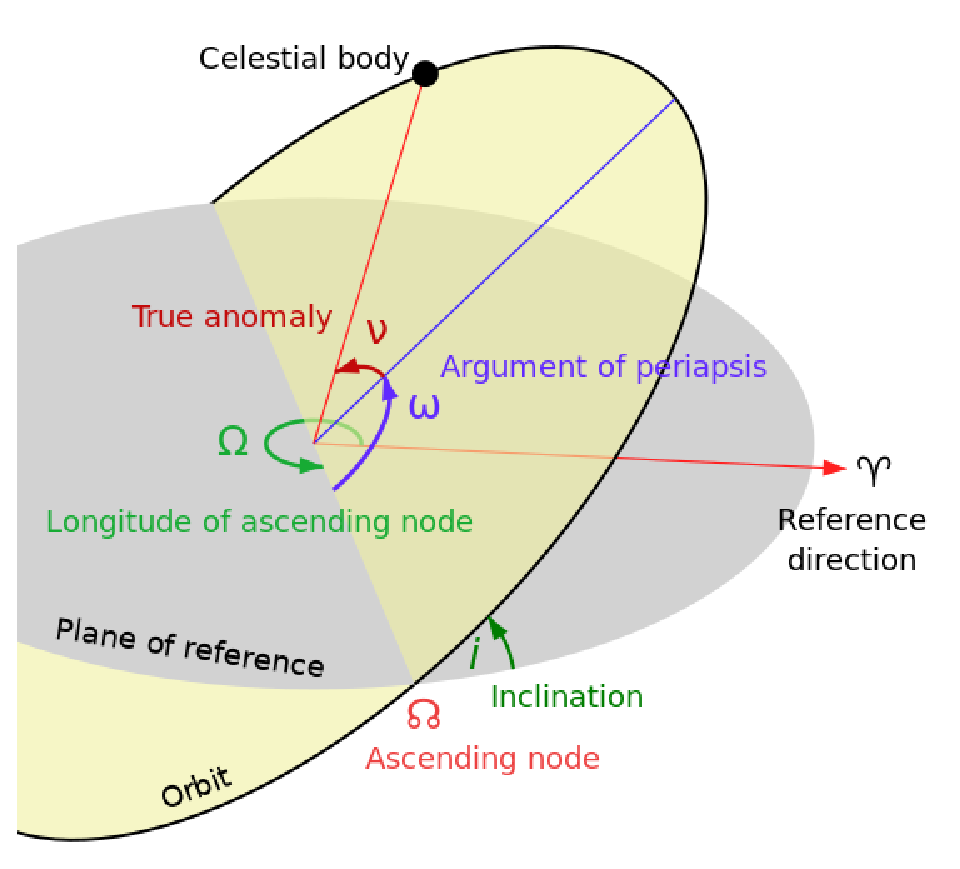
\includegraphics[]{4-images/keplerian_elements}
\caption{Visual representation of Keplerian elements. }
\label{keplerian_elements}
\end{figure}

Johannes Kepler published his first two laws about planetary motion in 1609, having found them by analysing the astronomical observations of Tycho Brahe. They are
%
\begin{enumerate}
    \item All planets move about the Sun in elliptical orbits, where the Sun in one of the foci.
    
    \item A line joining a planet to the Sun sweeps out equal areas in equal lengths of time.
\end{enumerate}
%
Kepler's third law was published later in 1619,
%
\begin{enumerate}
  \setcounter{enumi}{2}
    \item  The squares of the sidereal periods (of revolution) of the planets are directly proportional to the cubes of their mean distances from the Sun. 
\end{enumerate}
%
Any Keplerian trajectory in space can be characterised by a position vector and a velocity vector. Each of these has three components which change through an orbit. It is convenient to instead use \textit{Keplerian elements} - six parameters which can be used to calculate the position and velocity of an orbiting body. Two define the scale and  elongation of the orbit:
%
\begin{itemize}
\item $e$ - eccentricity,
\item $a$ - semi-major axis,
\end{itemize}
%
three define the orientation of the orbital plane:
%
\begin{itemize}
\item $i$ - orbital inclination, the angle between the orbital plane and the reference frame
\item $\Omega$- longitude of the ascending node which defines the angle between the reference direction and the upward crossing of the orbit on the reference plane,
\item $\omega$-argument of periapsis which defines the angle between the ascending node and the periapsis.
\end{itemize}
%
The position of the star(s) at a given time is specified by the following parameter
%
\begin{itemize}
\item $\nu$ - true anomaly which defines the position of the orbiting body along the trajectory, measured from periapsis.
\end{itemize}
%
A visual representation of Keplerian elements can be seen Fig. \ref{keplerian_elements}. The advantage of the Keplerian system over a Cartesian is that only one parameter changes through an orbit - $\nu$.

It is convenient to measure time relative to a reference time, $t_0$, that corresponds to a minimum in sky-projected separation between two stars (conjunction).   At time $t_o$ star 2 is closer to the observer than star 1. The true anomaly of star 1 at this time is $\nu_{1, t_0} \approx \pi /2 - \omega_0$. At other times, $t_i$, the true anomaly requires calculation of the time of periastron passage immediately prior to a given time of eclipse, $t_c$. The mean anomaly can then be calculated,
\begin{equation}
M = 2 \pi \frac{t_i - t_c}{P_a}
\end{equation}
where $P_a$ is the anomalistic period. Keplers law,
\begin{equation}
M = E - e \sin E
\end{equation}
and its differential form,
\begin{equation}
\frac{dM}{dE} = 1 - e \cos E
\end{equation}
can be used to solve for the eccentric anomaly, $E$, using the Newton-Raphson method. The true anomaly can then be calculated for star 1,
\begin{equation}
\nu_1 = 2 \tan ^{-1} \left[   \sqrt{\frac{1 + e}{1 - e}}  \tan (E/2)     \right]
\end{equation}
and $\nu_2 = \nu_1 + \pi$ for star 2. 




\subsection{Radial velocity}

The motion of each component in a binary system relative to the barycentre results in motion projected onto the line of sight. 
%The result is that a spectrum of each component appears more ``blue'' when the projected motion is towards the observer, and ``redder'' when moving in the opposite direction. This is akin to the Doppler effect; the change in pitch of an ambulance siren as it approaches and passes a static observer. 
We can obtain spectroscopic orbital parameters ($e$, $\omega$ and the semi-amplitude, $K_1$) by measuring
%how the spectrum shifts across an orbit. One approach is to measure the wavelength shift of a sharp, unblended line with respect to it’s laboratory wavelength. This provides a measurement of a star’s radial velocity via the Doppler effect equation:
%
%\begin{equation}\label{lambda_vrad}
%\frac{\Delta \lambda}{\lambda_0} = \sqrt{\frac{1 + %\frac{V_{\rm rad}}{c}}{1 - \frac{V_{\rm rad}}{c}}} .
%\end{equation}
%
%Repeating this procedure over many different lines and averaging provides an 
accurate radial velocities at several orbital phases and fitting a Keplerian orbit to these measurements. Another approach is look at the whole spectrum simultaneously. The wavelength shift, $\Delta \lambda$, is a function of radial velocity, $V_{\rm rad}$ , and the rest wavelength of a particular spectral line, $\lambda_0$. Hence an observed spectrum appears to shift by different amounts depending on the wavelength of the line that is measured. One way to overcome this is to convert from a linear wavelength scale to a natural logarithm wavelength scale:
%
\begin{eqnarray}
    \ln \left( \frac{\lambda}{\lambda_0} \right) & = \ln \lambda - \ln \lambda_0 \\
    & \approx \ln \left(1 + \frac{V_{\rm rad}}{c} \right).
\end{eqnarray}
%
Now a radial velocity shift, $V_{\rm rad}$, shifts the spectra along the $\ln \lambda$ axis, proportional to $V_{\rm rad}$ in a manner that is independent of $ \lambda_0$. With this known, we can employ the cross-correlation tool to compare a spectrum to a template spectrum of known radial velocity. A cross correlation is defined:
%
\begin{equation}
    c(x) = \int_{-\infty}^{\infty} f(\lambda) g(\lambda - x) d \lambda
\end{equation}
%
where for the independent variable, $x$, $c(x)$ is equal to the product of the two functions $f$ \& $g$, which are the programme spectrum and a template spectrum respectively. The function $c(x)$ is a measure of how well matched the two functions are over the range of displacement values, $x$. Providing the luminosity ratio between the two stars is not too extreme and the motion of each component along thee line of site is sufficiently different, there will be two peaks in $c(x)$ corresponding to each components moving towards and away from us. In EBLM systems, the FGK star dominates the light and only one peak will be measurable. These type systems which transit are also called single-lined eclipsing binaries (SB1s). It is beneficial to mask spectral features which may broaden/modify $c(x)$. The 8 EBLMs in this work with CORALIE spectra were cross-correlated with a numerical mask\footnote{``Spectrum'' of 0s and 1s at the position of spectral lines.} around Fe lines. The other EBLM with INT spectra masked the core of the H$\alpha$ line. Gaussian functions are often used to fit the peaks in $c(x)$ giving the relative radial velocity motion between the star and the template spectrum.



\begin{figure}
    \centering
    \includegraphics{4-images/radial_velocity_1.png}
    \caption{Example radial velocity models of the primary star for a circular orbit (solid), $e=0.2$ (dashed) and $e=0.4$ (dash-dot). The respective radial velocity models of the secondary stars are shown in light grey.}
    \label{theory:fig:radial_velocity_1}
\end{figure}

Calculating a model for the projected radial velocity ($V_{\rm rad}$) of star 1 at time $t_i$ is trivial once its true anomaly 1 ($\nu_{1,i}$)is calculated,
%
\begin{equation}\label{radial_velocity}
V_{\rm rad} = K_1 \left( e \cos \omega + \cos \nu_{1,i} + \omega \right) + \gamma\:\: \left[+ d(\gamma) / dt\right],
\end{equation}
%
where $K_1$ is the semi-amplitude and $\gamma$ is the systematic velocity of the binary system. Example radial velocity models are shown in Fig. \ref{theory:fig:radial_velocity_1}.  Unresolved faint companions in long-period orbits (tens of years) can introduce drifts in systematic velocity which require an extra term $d(\gamma) / dt$ to account for the inner-binary's orbit around the centre-of-mass. 

The SB1 nature of EBLMs mean that masses of each component cannot be calculated directly. The binary mass function, $f(m)$, can be used to constrain the the mass of the unseen component using parameters from Eqn. \ref{radial_velocity},
%
\begin{equation}\label{mass_function}
f(m)  =  \frac{(M_2 \sin i)^3}{(M_1 + M_2)^2} =  (1-e^2)^{\frac{3}{2}} \frac{P K_1^3}{2 \pi G}.
\end{equation}
%
The orbital inclination is generally not known but can be assumed to be near 90$^\circ$ if the binary system is transiting. In the case of exoplanets, $M_1 + M_2 \approx M_1$ which yields $M_2$ assuming prior knowledge of $M_1$ (e.g. from empirical relations) and inclination. It is important to note that $f(m) \propto K_1^3$ and any uncertainty in $K_1$ propagates by a factor of three into the mass function, and thus the masses of each star/planet. If the spectral lines of both stars can be measured it is possible to calculate the minimum masses of both components,
%
\begin{equation}
M_{1,2} \sin^3 i = c _m(1 - e^2)^{\frac{3}{2}} (K_1 + K_2)^2 K_{2,1} P
\end{equation}
%
where $c_m=1.0361 \times 10^{-7}\,M_\odot$ which is an up-to-date constant from IAU resolution B3 \citep{2016AJ....152...41P}. Similarly, the two semi-major axes of the orbits are,
%
\begin{equation}\label{theory:a}
a_{1,2} \sin i = c_a (1 - e^2)^{\frac{1}{2}}K_{1,2} P
\end{equation}
%
where $c_a = 1.9758 \times 10^{-2}\,R_\odot$.





\subsection{Light-curves}



\begin{figure}
    \centering
    \includegraphics[height=0.8\textheight]{4-images/transit_1.png}
    \caption{The primary eclipse for a uniformly illuminated star (solid), linear limb-darkened star ($c_1 = 0.6$; dashed) and a quadratically limb-darkened star ($c_1 = 0.6$, $c_2 = 0.4$; dash-dot) for impact parameters of $b = 0.0$ (top panel), $b=0.6$ (middle panel) and $b=0.8$ (lower panel). The contact points are marked in the top panel along with ingress/egress regions ($|\delta / R_\star - a| < k$; green) and when the apparent disk of star 2 is entirely encompassed by that of star 1 ($\delta / R_\star < 1-k$; blue). }
    \label{theory:fig:transit_1}
\end{figure}


\begin{figure}
\includegraphics[]{4-images/orbital_seperation}
\caption{The normalised orbital separation in terms of semi-major axis for a circular orbit inclined at $90^{\circ }$ (blue), an orbit with $e = 0.2$ at an inclination of $90^{\circ }$ (green-dashed) and an orbit with $e = 0.2$ at an inclination of $75^{\circ }$ (orange-dashed).}
\label{theory:fig:orbital_seperation}
\end{figure}


Knowledge of the Keplerian elements of an orbit permits the determination of the \textit{sky-projected separation},
%
\begin{equation}\label{sky_projected_seperation}
\delta = \frac{1 - e^2}{1 + e \cos \nu} \sqrt{1 - \sin^2i \sin^2(\nu + \omega)},
\end{equation}
%
where $\delta$ is normalised in terms of the semi-major axis, $a$. At this stage, it is convenient to introduce the radius of star 1 normalised in units of semi-major axis, $R_\star / a$, the ratio of the radii, $k = R_2 / R_\star$, and assume spherical star shapes. Dividing $\delta$ from Eqn. \ref{sky_projected_seperation} by $R_\star / a$ gives the projected sky separation in units of stellar radii. When $\delta / R_\star > 1 + k$, the projected sky-separation of each components disk is such that there is no overlap, and the light from each star is visible. However, when the projected sky-separation is such that $|\delta / R_\star - 1| < k$, there is a partial overlap between the disks of each star. For a primary eclipse (where star 2 is in-front of star 1), this would be the ingress/egress parts of a transit between contact points 1-2, and 3-4 (Fig. \ref{theory:fig:transit_1}). Between contact points 2-3 is where $\delta < 1 - k$ and the disk of star 2 sits entirely within the disk of star 1. 

The calculation of $\delta$ makes no assumption about the absolute position of each star. Over a single period for a transiting binary system, there are two occasions when $|\delta / R_\star - 1| < k$ (Fig. \ref{theory:fig:orbital_seperation}). Determining if a transit is a primary or secondary eclipse requires the calculation of the position for star 1 along the line of sight,
%
\begin{equation}
\bar{l} = \sin{ \left[ 2  \arctan{ \left[ \sqrt{\frac{1 + e}{1 - e}} \tan{\frac{E}{2}} \right] } + \omega \right] } \sin{i} . 
\end{equation} 
%
Instances where $\bar{l} > 0$ are primary eclipses (star 2 in front of star 1) and $\bar{l} < 0$ are secondary eclipses. For systems with low values of $k$, the entirety of the secondary star is obscured in secondary eclipses leading to a flat-bottomed eclipse. The shape of the secondary eclipse is typically parameterised by the surface brightness ratio, $S = k^2 F_{\lambda,2} / F_{\lambda,\star}$, where $F_{\lamda}$ is the flux of each star observed in some bandpass. The depth of a secondary eclipse is then given by $1-S \times k^2$.   


\subsection{Limb darkening}

% look here
% http://iopscience.iop.org/article/10.1086/346105/pdf

\begin{figure}
\includegraphics[scale = 0.5]{4-images/imb_darkening}
\caption{(top) An image obtained from the Solar Dynamics Observatory on March $3^{rd}$ 2018, 01:04:29 UT using the 1700\AA filter. (bottom) The normalised intensity profile of the Sun using the SDO 1700\AA image (top).  }
\label{theory:fig:SDO_1700A}
\end{figure}

Creating a model for an eclipse would be trivial if the disc of each star was uniformly illuminated. In this case, the drop in flux would be proportional the area occulted on the furthest star by the nearest star. This would result in transits where all contact points would be easily discernible and the flux between contact points 2 and 3 would be constant. Unfortunately,  lightcurves taken in filters blueward of $\sim 1 \mu m$ show a slight ``rounding'' of the lightcurve caused by stars emitting more light at the centre than the edge (limb); this is called limb darkening. The reason for this is that light occulted near the limbs originates from a colder column of gas which emits less light than a hotter column of gas near the centre of the disk. This can be seei in an image of the Sun from the Solar Dynamics Observatory (Fig. \ref{theory:fig:SDO_1700A}) which shows a clear drop in light emmited toward the edge of the solar disk.  This intensity across a stellar disk is typically defined in terms of $\mu = \cos \gamma$, where $\gamma$ is the angle between a line normal to the stellar surface and the line of sight. How the normalised intensity $I(\mu)/I_0$ is related to $\mu$ largely remains a task for theoreticians since very few stars are resolvable (see Altair \citealt{2007Sci...317..342M}; $\pi^1$ Gruis \citealt{2018Natur.553..310P}; Betelgeuse \citealt{1998AJ....116.2501U}; Antares \citealt{2017Natur.548..310O} \ldots) and provide little or no constraints on surface intensity distributions across different spectral types.

As stated by \citet{2002astro.ph.10076S}, the generel effect of limb darkening is to (1) change the depth of the lightcurve as a function of impact parameter, where the transit is deeper for most values of impact parameter, (2) make the flat bottom between contact points 2 and 3 rounder and (3) blur the boundary between contact points 2 and 3. These effects are show in Fig. \ref{theory:fig:transit_1}. There are a number of limb-darkening laws used to describe how $I(\mu)/I_0$ changes with $\mu$. These largely depend on a series of coefficients, $c_i$, depending on the number of parameters. Some examples are,
%
\begin{eqnarray}
I(\mu)/I_0 & = 1 - c_1(1 - \mu) & \rm [Linear]\footnotemark\\
I(\mu)/I_0 & = 1-c_1(1-\mu) - c_2(1 - \mu)^2 & \rm [quadratic]\footnotemark \\
I(\mu)/I_0 & = 1 - c_1 (1 - \mu) - c_2 (1 - \sqrt{\mu}) & \rm [square \text{-} \rm root]\footnotemark \\
I(\mu)/I_0 & = 1 - c_1 (1 - \mu) - c_2 \mu \log \mu & \rm [logarithmic]\footnotemark \\
I(\mu)/I_0 & = 1 - c_1 ( 1 - \mu) - \frac{c_2}{1 - \exp{\mu}} & \rm [exponential]\footnotemark \\
I(\mu)/I_0 & = 1 - c_1 (1 - \mu) - c_2 ( 1 - \mu^{\frac{3}{2}}) - c_3 (1 - \mu^2) & \rm [sing]\footnotemark \\
I(\mu)/I_0 & = 1 - c_1 (1 - \mu^{c_2}) & \rm [power \text{-} \rm 2]\footnotemark \\
I(\mu)/I_0 & = 1 - c_1(1 - \mu^{\frac{1}{2}}) - c_2 (1 - \mu) - c_3 (1 - \mu^{\frac{3}{2}}) - c_4 (1 - \mu^2) & \rm [claret]\footnotemark .
\end{eqnarray}
%
\addtocounter{footnote}{-7}
\footnotetext{\citet{1906MiGoe..13....1S}}
\stepcounter{footnote}
\footnotetext{\citet{1950HarCi.454....1K}}
\stepcounter{footnote}
\footnotetext{\citet{1992A&A...259..227D}}
\stepcounter{footnote}
\footnotetext{\citet{1970AJ.....75..175K}}
\stepcounter{footnote}
\footnotetext{\citet{2003A&A...412..241C}}
\stepcounter{footnote}
\footnotetext{\citet{2009A&A...505..891S}}
\stepcounter{footnote}
\footnotetext{\citet{1997A&A...327..199H}}
\stepcounter{footnote}
\footnotetext{\citet{Claret2000}}
%
Many of these limb-darkening laws have tables of coefficients ($c_i$) for a given set of stellar atmospheric parameters ($T_{\rm eff}$, [Fe/H] and $\log g$). I used the Claret 4-parameter law to fit the lightcurves of 5 EBLMs observed from ground-based instruments by interpolating coefficients for a given limb-darkneing temperature. I used the power-2 law to measure 4 EBLMs observed with K2 by fitting the coefficients, $c_i$, as free parameters (see Sect. \ref{method:orbital_fit}). To model secondary eclipses I assumed that the M-dwarf is uniformly illuminated and use the analytical expression presented by \citet{2015PASP..127.1161K}. 


\section{Absolute parameters}

Transit photometry parameters ($R_\star / a$, $k$ \& $i$) sets the radii scale of the system whilst radial velocity parameters ($K_1$ \& $e$) set the mass scale between the components. Often, we are more interested in dimensional parameters such as the mass of each companion, or the semi-major axis in astronomical units. For those, the orbital solution (best-fitting transit and radial velocity parameters) must be combined with supplementry information such as the mass or radius of the primary star obtained by other means (e.g. stellar parallax, spectrum or angular diameter; \citealt{2009IAUS..253...99W}). A brief description on how masses, radii and age are interpolated in this work, and across the field, is given in Sect. \ref{methods:eblmmass}. However, two important parameters can be calculated from the orbital solution directly. 

$\log g_2$ of the secondary star can be obtained by combining the mass function (Eqn. \ref{mass_function}) with the mathematical expression of Keplers third law,
%
\begin{equation}\label{Kepler3}
    \frac{P^2}{a^3} = \frac{4 \pi ^2}{G ( M_\star + M_2)},
\end{equation}
%
it is possible to solve for the sum of the masses of the two components,
%
\begin{equation}\label{mass_sum}
    (M_\star + M_2)^2 = \frac{2 \pi G M_2^3 \sin^3 i}{(1-e^2)^{3/2} K_1^3 P} = \frac{(2 \pi)^4 a^6}{G^2 P^4}.
\end{equation}
%
By substituting $R_2 = a r_2$, where $r_2 = R_2 / a$, into the definition of surface gravity and replacing $a$ using Eqn. \ref{mass_sum}, the surface gravity of star 2 can be calculated:
%
\begin{equation}\label{suface_gravity}
    g_2 = \frac{2 \pi}{P} \frac{\sqrt{1 - e^2} K_1}{r_2^2 \sin i}.
\end{equation}
%


Density of the primary star, $\rho_\star$, can also be calculated from the total transit duration assuming a circular orbit,
%
\begin{equation}\label{transit_duration}
    t_T = \frac{P}{\pi} \arcsin \left( \frac{R_\star}{a} \sqrt{\frac{(1 + k)^2 - b^2}{1 - \cos^2 i}} \right).
\end{equation}
%
By combining Eqn. \ref{Kepler3} with Eqn. \ref{transit_duration} it is possible to calculate the stellar density,
%
\begin{equation}\label{mean_density}
    \rho_\star \equiv \frac{M_\star}{\frac{4}{3} \pi R_\star^3} = \frac{3 \pi}{G P^2} \left( \frac{a}{R_\star} \right)^3 - \frac{M_2}{R_\star^3}.
\end{equation}
%
For exoplanets ($M_\star >> M_2$), the second term on the right-hand side of Eqn. \ref{mean_density} can be ignored to give a robust estimate of the stellar density. For EBLMs systems, the mass ratio $q = M_2 / M_\star \approx 0.1$-$0.6$ and so Eqn. \ref{mean_density} requires further constraints on masses and radii. 



% Chapter 5. Wavelet analysis
%\chapter{Atmospheric parameters of FGK stars using wavelet analysis}\label{chapter:wavelet}

As part of the WASP exoplanet follow-up procedure, 10+ spectra were obtained for candidate exoplanets to estimate the semi-amplitude ($K$) and mass ratio ($q$). In subsequent years, more spectra of EBLMs were obtained from the CORALIE \'{e}chelle spectrograph \citep{2001Msngr.105....1Q} as part of the EBLM project. This lead to the publication of spectroscopic orbits for over 100 EBLM systems \citep{Triaud2017}. \citet{Triaud2017} use photometric colours to determine the effective temperature of the host star. The individual analysis of each spectrum is acceptable for a small sample size, but we require a reliable automated procedure to measure $T_{\rm eff}$, [Fe/H] and V$\sin i$ for the entirety of the EBLM database to keep pace with future EBLM discoveries.

Accurate measurements of temperature and composition are needed to estimate limb-darkening coefficients and the mass of the primary the star. For EBLM systems discovered by WASP, these parameters are usually made with CORALIE spectra using measurements of equivalent widths and by fitting individual spectral lines (\citealt{2009A&A...496..259G}; \citealt{Doyle2013}; \citealt{Doyle2015}). At the same time, such a method needs to allow for noise and systematic errors present in the CORALIE spectra. The sample of EBLM spectra presented in \citet{2014A&A...572A..50G} typically have a signal-to-noise ratio per $\AA$ngstrom (SNR) between 3 and 7. The on-going radial velocity campaign to study EBLMs typically yields between 10 and 40 spectra per star. Co-adding spectra can increase the SNR ($\propto \sqrt{N_{\rm obs}}$) to over 40 in some parts of the spectrum, but the regions of the spectrum near the ends of each \'{e}chelle order suffer from both large photon noise and systematic errors due to inaccurate order-merging.  

Wavelet decomposition has been used previously as part of methods developed for spectral analysis. \citet{2010PASP..122..608M} used multi-level wavelet decomposition in connectionist systems (artificial neural networks) to derive fundamental stellar parameters in the low SNR domain (5-25) in preparation for spectra from the Gaia radial velocity spectrograph (RVS). This work was extended by \citet{2016A&A...594A..68D} by using a generative artificial neural network resulting in predicted uncertainties of 220\,K, 0.32\,dex and 0.20\,dex for T$_{\rm eff}$, $\log g$ and [Fe/H], respectively for stars with a Gaia magnitude $G_{RVS}$ = 13. Using neural networks to estimate atmospheric properties has well-known problems such as long training times and a strong dependence on the initial training set. \citet{2015ApJS..218....3L} use wavelet decomposition in a regression framework to detect representative spectral features from a set of 30,000 SDSS spectra to estimate atmospheric parameters with better precision than those from neural network (83\,K, 0.23\,dex
and 0.16\,dex for T$_{\rm eff}$, $\log g$ and [Fe/H]).

The method in this work determines the best-fitting atmospheric parameters ($T_{\rm eff}$, $\log g$, [Fe/H] and V$\sin i$) for EBLM host stars by comparing a selected subset of coefficients from a wavelet decomposition to those from a grid of stellar models. This reduces systematic errors in the estimated parameters due to poor continuum normalisation and low-quality regions of the spectrum. These measurements can then be combined with photometric follow-up observations to obtain the mass and radius of M-dwarfs in EBLMs to an accuracy of a few percent. These, in turn, provide calibratable points for empirical mass-radius relations of low-mass stars (e.g. \citealt{2009A&A...505..205D}; \citealt{2010A&ARv..18...67T}). We introduce wavelet decomposition as it applies to a spectrum in Sect. \ref{wavelet:wavelet_decomposition} before reviewing my Bayesian approach to determine $T_{\rm eff}$, [Fe/H], $\log g$ and $V \sin i$ in Sect. \ref{wavelet:Method}. We show that my method converges and is self-consistent in Sect. \ref{wavelet:self_con} and test against a sample of independently analysed FGK stars in Sect. \ref{wavelet:wavelet_benchmark}. This work is published in Astronomy \& Astrophysics \citep{2018A&A...612A.111G}.  


\section{Wavelet decomposition theory}\label{wavelet:wavelet_decomposition}

\begin{figure*}[ht!]
\centering
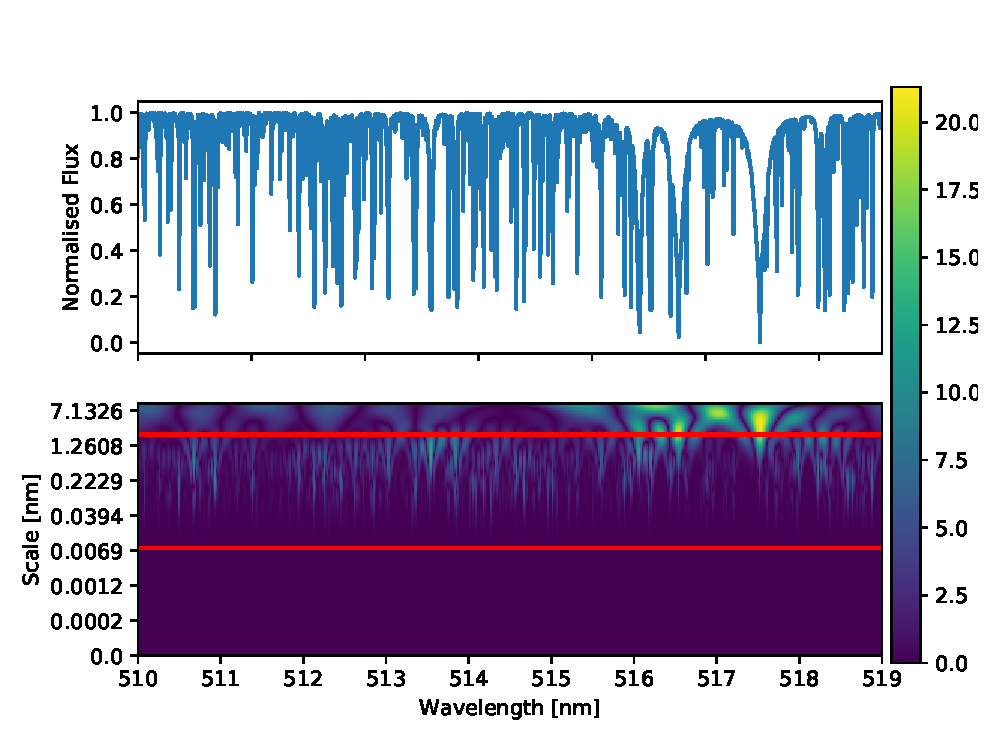
\includegraphics[width=0.95\textwidth]{5-images/wavelet_power.eps}
\caption{The power H\"{o}vmoller of wavelet coefficients (lower panel) for a region around the Mg triplet for WASP-19 (upper panel). There is significant power ($|WT_{i,k}|$ from Eq. \ref{DWT}) for scales $\sim$1\,nm in the region of the Mg lines corresponding the wavelets likeness to spectral features. Horizontal red lines represent the scales $0.012-3.125$\,nm.}
\label{fig:wavelet:wavelet_power}
\end{figure*}


\begin{figure*}
\centering
\begin{subfigure}{.5\textwidth}
  \centering
                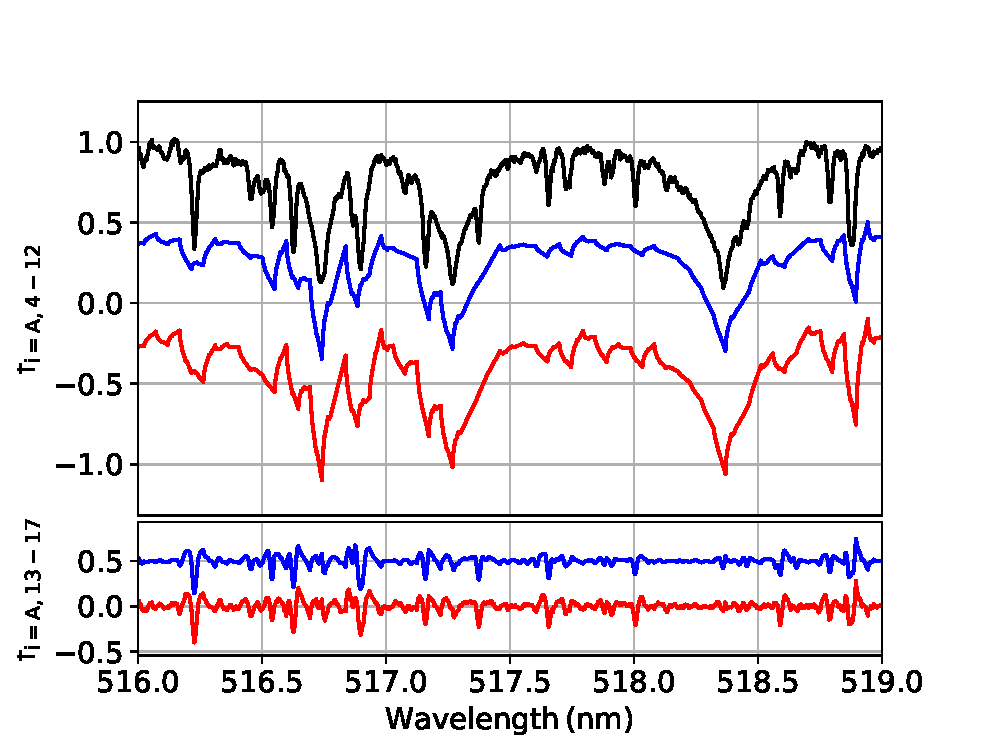
\includegraphics[width=0.9\textwidth]{5-images/waveletfilter_bad.eps}
                \caption{}\label{filt:a}
\end{subfigure}%
\begin{subfigure}{.5\textwidth}
  \centering
                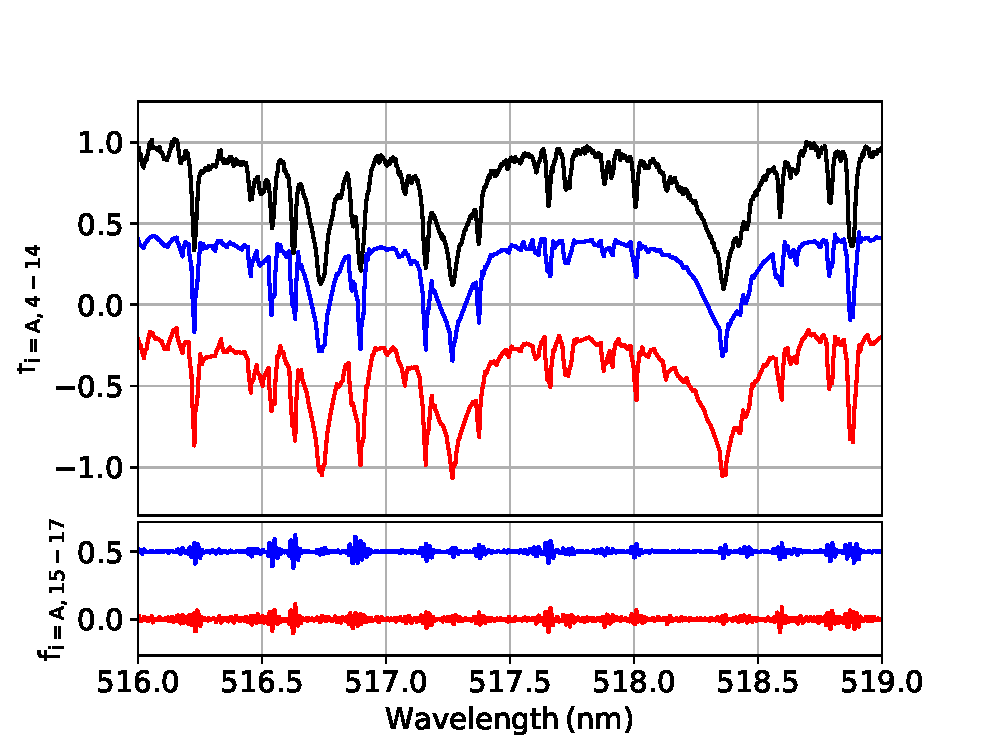
\includegraphics[width=0.9\textwidth]{5-images/waveletfilter.eps}
                \caption{}\label{filt:b}
\end{subfigure}
\caption{The reconstruction of spectra using Eq. (\ref{IDWT}) for subsets of wavelet coefficients. (Left panel - top) Raw spectra for WASP-19 (black) and the flux reconstruction using wavelet coefficients from bands $i=4$-$12$ using the raw spectrum (blue; offset $-0.6$) and the best fitting model for WASP-19 (red; offset $-1.2$). (Left panel - bottom) The reconstruction of the best-fitting model for WASP-19 (red) and the raw spectrum (blue; offset $+0.5$) using coefficients $i=13$-$17$. (Right panel) As in the left panel except with reconstructions using coefficients $i=4$-$14$ (top) and coefficients $i=15$-$17$ (bottom).}\label{fig:wavelet:filt}
\end{figure*}

Analysis of spectral components at different scales can be done using a discrete wavelet transform (DWT). A DWT tiles the wavelength-scale plane by convolving a spectrum, $f( \lambda )$, with variable sized functions \citep{2012AAS...22033004S}. These functions are called daughter wavelets, $\psi_{\rm a,b}(\lambda)$, which are created from a mother wavelet, $\psi(\lambda )$,  using a shift-and-scale operation,
%
\begin{equation}\label{daugthermother}
\psi_{a,b}(\lambda) = \frac{1}{\sqrt{a}}\psi(\frac{\lambda - b}{a}),\quad a,b \in  \Re, a \neq 0 ,
\end{equation}
%
where  $a$ is a member of the dyadic sequence,
%
\begin{equation}\label{dyadic}
a_{i} = 2^{i}, \quad i = 0,1,2,3,...,n
\end{equation}
%
and $b=kb_{0}$, where $k$ is an integer and $b_0$ is chosen to ensure the recovery of $f(\lambda)$. By employing a DWT, the appropriate values of $b$ are selected to minimise overlap between wavelet convolutions. Following the notation in chapter 8 of \citet{Olkkonen2011}, a discrete wavelet transform can be calculated for each dyadic scale ($i$) and displacement ($k$):
%
\begin{equation}\label{DWT}
WT_{f(\lambda)}(i,k) = \frac{1}{\sqrt{2^i}} \int f(\lambda)\overline{\psi \left(\frac{\lambda - k2^ib_0}{2^i} \right)} d\lambda = f(\lambda),\psi_{i,k}(\lambda)
.\end{equation}
%
The likeness of a wavelet, $\psi_{i,k}$, to a section of the spectrum is given by the wavelet coefficient $WT_{f(\lambda)}(i,k)$ from Eq. (\ref{DWT}). Performing this calculation over the series of dyadic scales and displacements yields wavelet coefficients which represent different sized structures at different wavelengths. I split coefficients into bands with constant scales, $\lbrace WT_{f(\lambda)}(0,b)\rbrace_k$, which represent the likeness of a single scale across the entire spectrum. The power of each scale, $\lbrace WT_{f(\lambda)}(i,b)\rbrace_k^2$ , can be visualised in a power H\"{o}vmoller (one value of $i$ per row) in Fig. \ref{fig:wavelet:wavelet_power}. Bands of coefficients which correspond to noise and low-order continuum artefacts (such as merged \'{e}chelle orders) can then be excluded. A filtered spectrum may be reconstructed with an inverse DWT (IDWT):
%
\begin{equation}\label{IDWT}
f(\lambda) = \sum_{i=-\infty }^{\infty} 2^{\frac{-3i}{2}} \int WT_{f(\lambda)}(i,k)\hat{\psi} \left(\frac{\lambda - b}{2^i} \right)db
,\end{equation}
%
where
%
\begin{equation}
\hat{\psi} \left(\frac{\lambda - b}{2^i} \right) = \frac{\psi \left(\frac{\lambda - b}{2^i} \right)}{\sum_{i=0}^{i=n} \left| \psi \left(\lambda - b \right) \right|^2 }
.\end{equation}
%
The process of reconstructing a spectrum using a subset of wavelet coefficients is called wavelet filtering and is analogous with Fourier filtering. Alternatively, the subset of coefficients may be chosen to meet a threshold criteria (i.e. $\left[ WT_{f(\lambda)}(i,k) \right]^2  \geq \rm 0.01$) which eliminates information that has little contribution to a signal; this is called wavelet compression.

I do not require Eq. (\ref{IDWT}) to determine atmospheric parameters as I perform a $\chi^2$ fit using a subset of coefficients from Eq. (\ref{DWT}) to those from a grid of models (see Sect. \ref{wavelet:Method}). I also do not apply any threshold criterion. The nominal resolving power of the CORALIE spectrograph is R=55\,000, so at least $2^{16}$ values are required to sample a spectrum over the wavelength range 450-650nm.  I decided to use $2^{17}$ values for the wavelet decomposition to ensure no loss of information and to give us more choice in the number of wavelet bands used in my analysis. I used Eq. (\ref{DWT}) to obtain wavelet coefficients which have information on scales in the range 0.003\,nm--200\,nm. My wavelet method only uses a subset of $i$ values. To select these, I constructed power H\"{o}vmoller diagrams (similar to Fig. 1) for a variety of regions between 450\,nm and 650\,nm, for different co-added spectra in my sample. I found that power associated with line absorption lies in the range 0.04--4\,nm, with larger scales typically corresponding to systematic trends and shorter scales with noise. This corresponds to values of i=4--12 (0.048--3.125\,nm).  The application of Eq. (\ref{IDWT}) to the two subsets of coefficients (4--12 and 13--17) is shown in Fig. \ref{filt:a}.  I found that the subset range $i=4-12$ is too restrictive  to reproduce short-scale information (e.g. weak lines) and so I decide to extend this range to $i=4-14$ (0.012--3.125\, nm; Fig. \ref{filt:b}) which better represents the boundary between noise and weak lines. I do not show the reconstruction of subset $i=0-3$ in Fig. \ref{filt:a} and \ref{filt:b} as using only 16 coefficients to reconstruct a spectrum leads to a large Daubechies-4 wavelet with some sub-structure.  


I demonstrate the sensitivity of wavelet coefficients to atmospheric parameters in Fig. \ref{fig:wavelet:wavelet_power} for wavelet coefficients in the range $i=11-12$ ($0.04\,-\,0.09\, \rm nm$). I see a slow variation of some wavelet coefficients which corresponds to changes in individual spectral line geometries as each parameter changes.  One thing to note is the sensitivity of each parameter; $T_{\rm eff}$ varies the most, followed by $V \sin i$ and [Fe/H]. Surface gravity is the least varying parameter in wavelet space and is dominated by a few lines sensitive to $\log g$. As $V \sin i$ increases, I see positive and negative structures form and become stronger at higher $V \sin i$ values. This is likely to be a continuum effect as weaker lines are smeared out to average a lower continuum whilst stronger lines persist.

The choice of mother wavelet depends on the objective of the work.  A Daubechies wavelet performs well for frequency identification and is widely used in signal processing and data compression \citep{2002A26A...386.1143B}. A Haar wavelet, with a more step-like structure, is more suited to identifying discontinuity and is widely used in computer-vision projects (e.g. \citealt{2009arXiv0911.0399E}). I investigate the effects of wavelet choice on the determined atmospheric parameters in Sect. \ref{wavelet:fe_offset}, but proceed with the Daubechies ($k$=4) wavelet for the rest of this work. 


\section{Bayesian measurements} \label{wavelet:Method}


\begin{figure}[ht!]
\centering
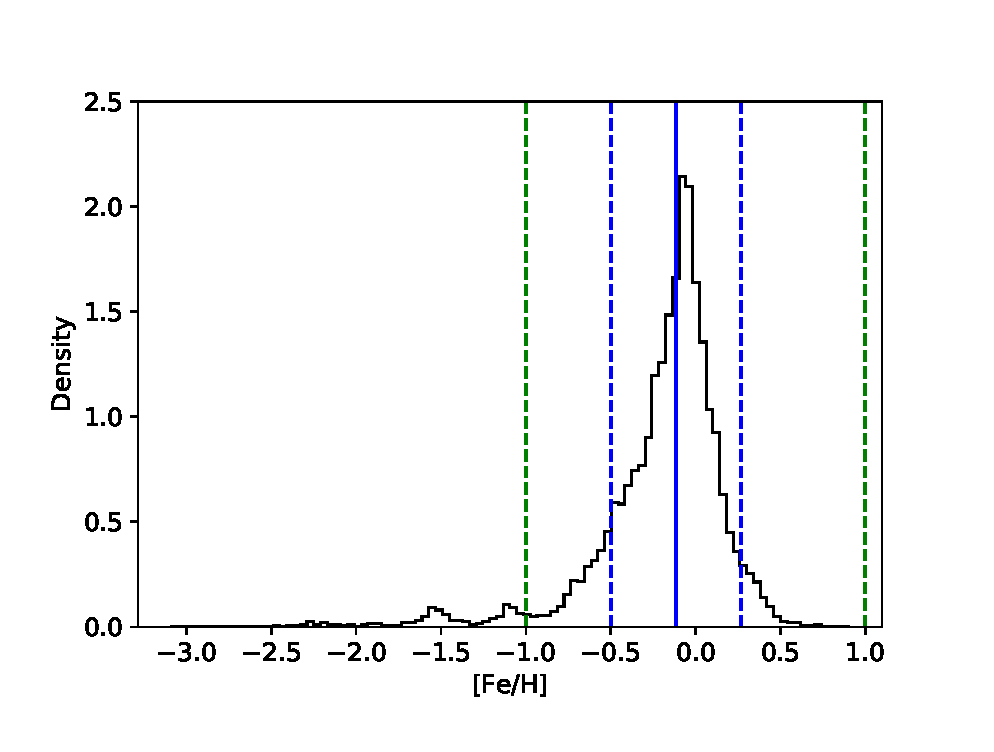
\includegraphics[scale=1]{5-images/FEH_FGK_stars.eps}
\caption{Histogram of 14,681 [Fe/H] measurements for  stars from Gaia-ESO data release 3 \protect\citep{2014A&A...570A.122S}. Plotted is the median value of [Fe/H] (solid blue), with $1 \sigma$ from the median (dashed blue). The grid range used in enclosed by the dashed green lines.}
\label{wavelet:fig:FE_H}
\end{figure}

I use the Markov chain Monte Carlo method to determine the posterior probability distribution for $T_{\rm eff}$, $\log g$, $V \sin i$ and [Fe/H] given an observed spectrum. My method is a global $\chi^2$ fitting routine which compares subsets of wavelet coefficients ($i=4-14$) to those from a pre-synthesised grid of spectra. My grid was synthesised with the radiative transfer code SPECTRUM \citep{1994AJ....107..742G} using MARCS model atmospheres \citep{2008A&A...486..951G}, and version 5 of the GES (GAIA ESO survey)  atomic line list provided within iSpec \citep{2016csss.confE..22B} with solar abundances from \cite{2009ARA&A..47..481A}. I computed models spanning 450nm--650nm over a temperature range of 4000 to 8000\,K in steps of 250K, $-$1 to +1\,dex in steps of 0.5 dex for [Fe/H] and 3.5 to 5\,dex in steps of 0.5 for $\log g$. I selected the range of [Fe/H] by looking at composition measurements of over 14,000 FGK stars from Gaia-ESO survey data release 3 (Fig. \ref{wavelet:fig:FE_H}; \citealt{2014A&A...570A.122S}). I found that 96\% of stars with measurements of composition had [Fe/H] in the range $-$1 to 1\,dex. This range in [Fe/H] is also much larger than the full  range in [Fe/H] for the benchmark sample described in Sect. \ref{wavelet:wavelet_benchmark}. 


Spectra in the grid are calculated with zero instrumental, rotational, or macroturbulence broadening. These are accounted for in post-processing by convolving the grid spectra with the appropriate kernels. In this work, I allow $V \sin i$ to have values in the range $0$ - $50 \, \rm kms^{-1}$. The upper limit of $50\,kms^{-1}$ would need to be extended for hotter stars beyond the Kraft break, but is suitable for this work on late-type stars. Macroturbulence are estimated using Eq. (5.10) from \citet{Doyle2015} and microturbulence was accounted for at the synthesis stage using Eq. (3.1) from the same source. Spectra in-between grid points are extracted by trilinear interpolation, broadened to the desired value of $V \sin i$ and macroturbulence, and then convolved with a Gaussian to account for  instrumental broadening. For the self-consistency tests in Sect. \ref{wavelet:self_con} instrumental broadening was ignored, but for the CORALIE spectra in Sect. \ref{wavelet:wavelet_benchmark} I used an instrumental resolving power $R = 55,000$ \citep{2001Msngr.105....1Q,Doyle2015}. I then re-sample between 450\,and 650\,nm with 2$^{17}$ values (the same as the observed spectrum) and apply Eq. (\ref{DWT}) to obtain the wavelet coefficients $WT_{f(\lambda)}(4-14,k)$ for the model spectra. 

The subset of wavelet coefficients from the interpolated model, $WT_{\textbf{m}}$, are compared to those from the data, $WT_{\textbf{d}}$, in the following Bayesian framework: the probability of observing a spectrum for a given model is given by $\rm p(\textbf{m}|\textbf{d})\propto \mathcal{L}(\textbf{d}|\textbf{m}) \rm p(\textbf{m})$. The vector of model parameters  is given by $\rm \textbf{m} = \left( \rm T_{\rm eff}, \rm [Fe/H], \log g, \rm V \sin i \right)$ and I assume uniform prior probability for the model parameters within the grid range. I use the likelihood function $\mathcal{L}(\textbf{d}|\textbf{m}) = \exp (-\chi^2/2)$ where

\begin{equation}\label{chi_squared}
\chi^{2} = \frac{(WT_{\textbf{d}} - WT_{\textbf{m}})^{2}}{\sigma_{WT_{\textbf{d}}}^2}
,\end{equation}
and 

\begin{equation}\label{sigma}
\sigma_{WT_{\textbf{d}}}^2 = \beta \sigma_{MC}^{2}.
\end{equation}
The term $\sigma_{MC}^{2}$ was calculated by generating 1000 spectra from the co-added spectrum with noise generated from a standard normal distribution centred around $f(\lambda)$ and with $\sigma$ equal to the standard deviation of the spectrum, $\sigma_{f(\lambda)}$ (calculated from the standard deviation in co-added spectra). The blaze function is corrected prior to co-addition of the spectra and so deviations in blaze functions will result in uncertainties propagating through to $\sigma_{f(\lambda)}$, and $\sigma_{MC}^{2}$, effectively down-weighting regions with poor blaze corrections.  The free parameter $\beta$ has been introduced to account for additional noise, incomplete atomic data, deviations from solar metallicity scaling, lines which form under non-local thermodynamic equilibrium, and other unaccounted errors. In principle, I could have used stellar models or empirical relations to set priors on these atmospheric parameters but decided not to do this for two reasons. Firstly, allowing the MCMC sampler to explore regions with a-priori low probability gives a better indication of the reliability of my method than using a more constrained solution. Secondly, by imposing a prior from stellar models or empirical relations based on normal stars we may fail to identify interesting examples of anomalous stars in my sample, for example, helium-rich stars. 
I sample the model parameter space using the Markov chain Monte Carlo method, implemented by the python package {\sc{emcee}} \citep{2013PASP..125..306F} . {\sc{emcee}} uses affine-invariant ensemble sampling (parallel stretch move algorithm; \citealt{Goodman2010}) to split Markov chains into sub-groups and update the position of a chain using the positions of chains in the other subgroups. The algorithms affine-invariance can cope with skewed probability distributions and generally has shorter autocorrelation times than a classic Metropolis-Hastings algorithm.

I generate 12 Markov chains of 20,000 draws each to converge on the best atmospheric parameters. I found that the chains converged before the 5000$^{th}$ draw, but as a precaution I discarded the first 10,000 draws. I take the median values of the model parameters in the remaining draws to determine the atmospheric parameters for a spectrum. An example posterior probability distribution for WASP-20 is plotted in Fig. \ref{fig:wavelet:wavelet_corner_WASP20}. The parameter space is almost symmetric with small degeneracies between $T_{\rm eff}$, [Fe/H] and $\log g.$ I note that the precision of the parameters determined from the standard deviation of each parameter in the Markov Chain is typically an underestimate of the true precision of these parameters because it does not account for systematic errors in the data or the models.

\begin{figure*}[ht!]
\centering
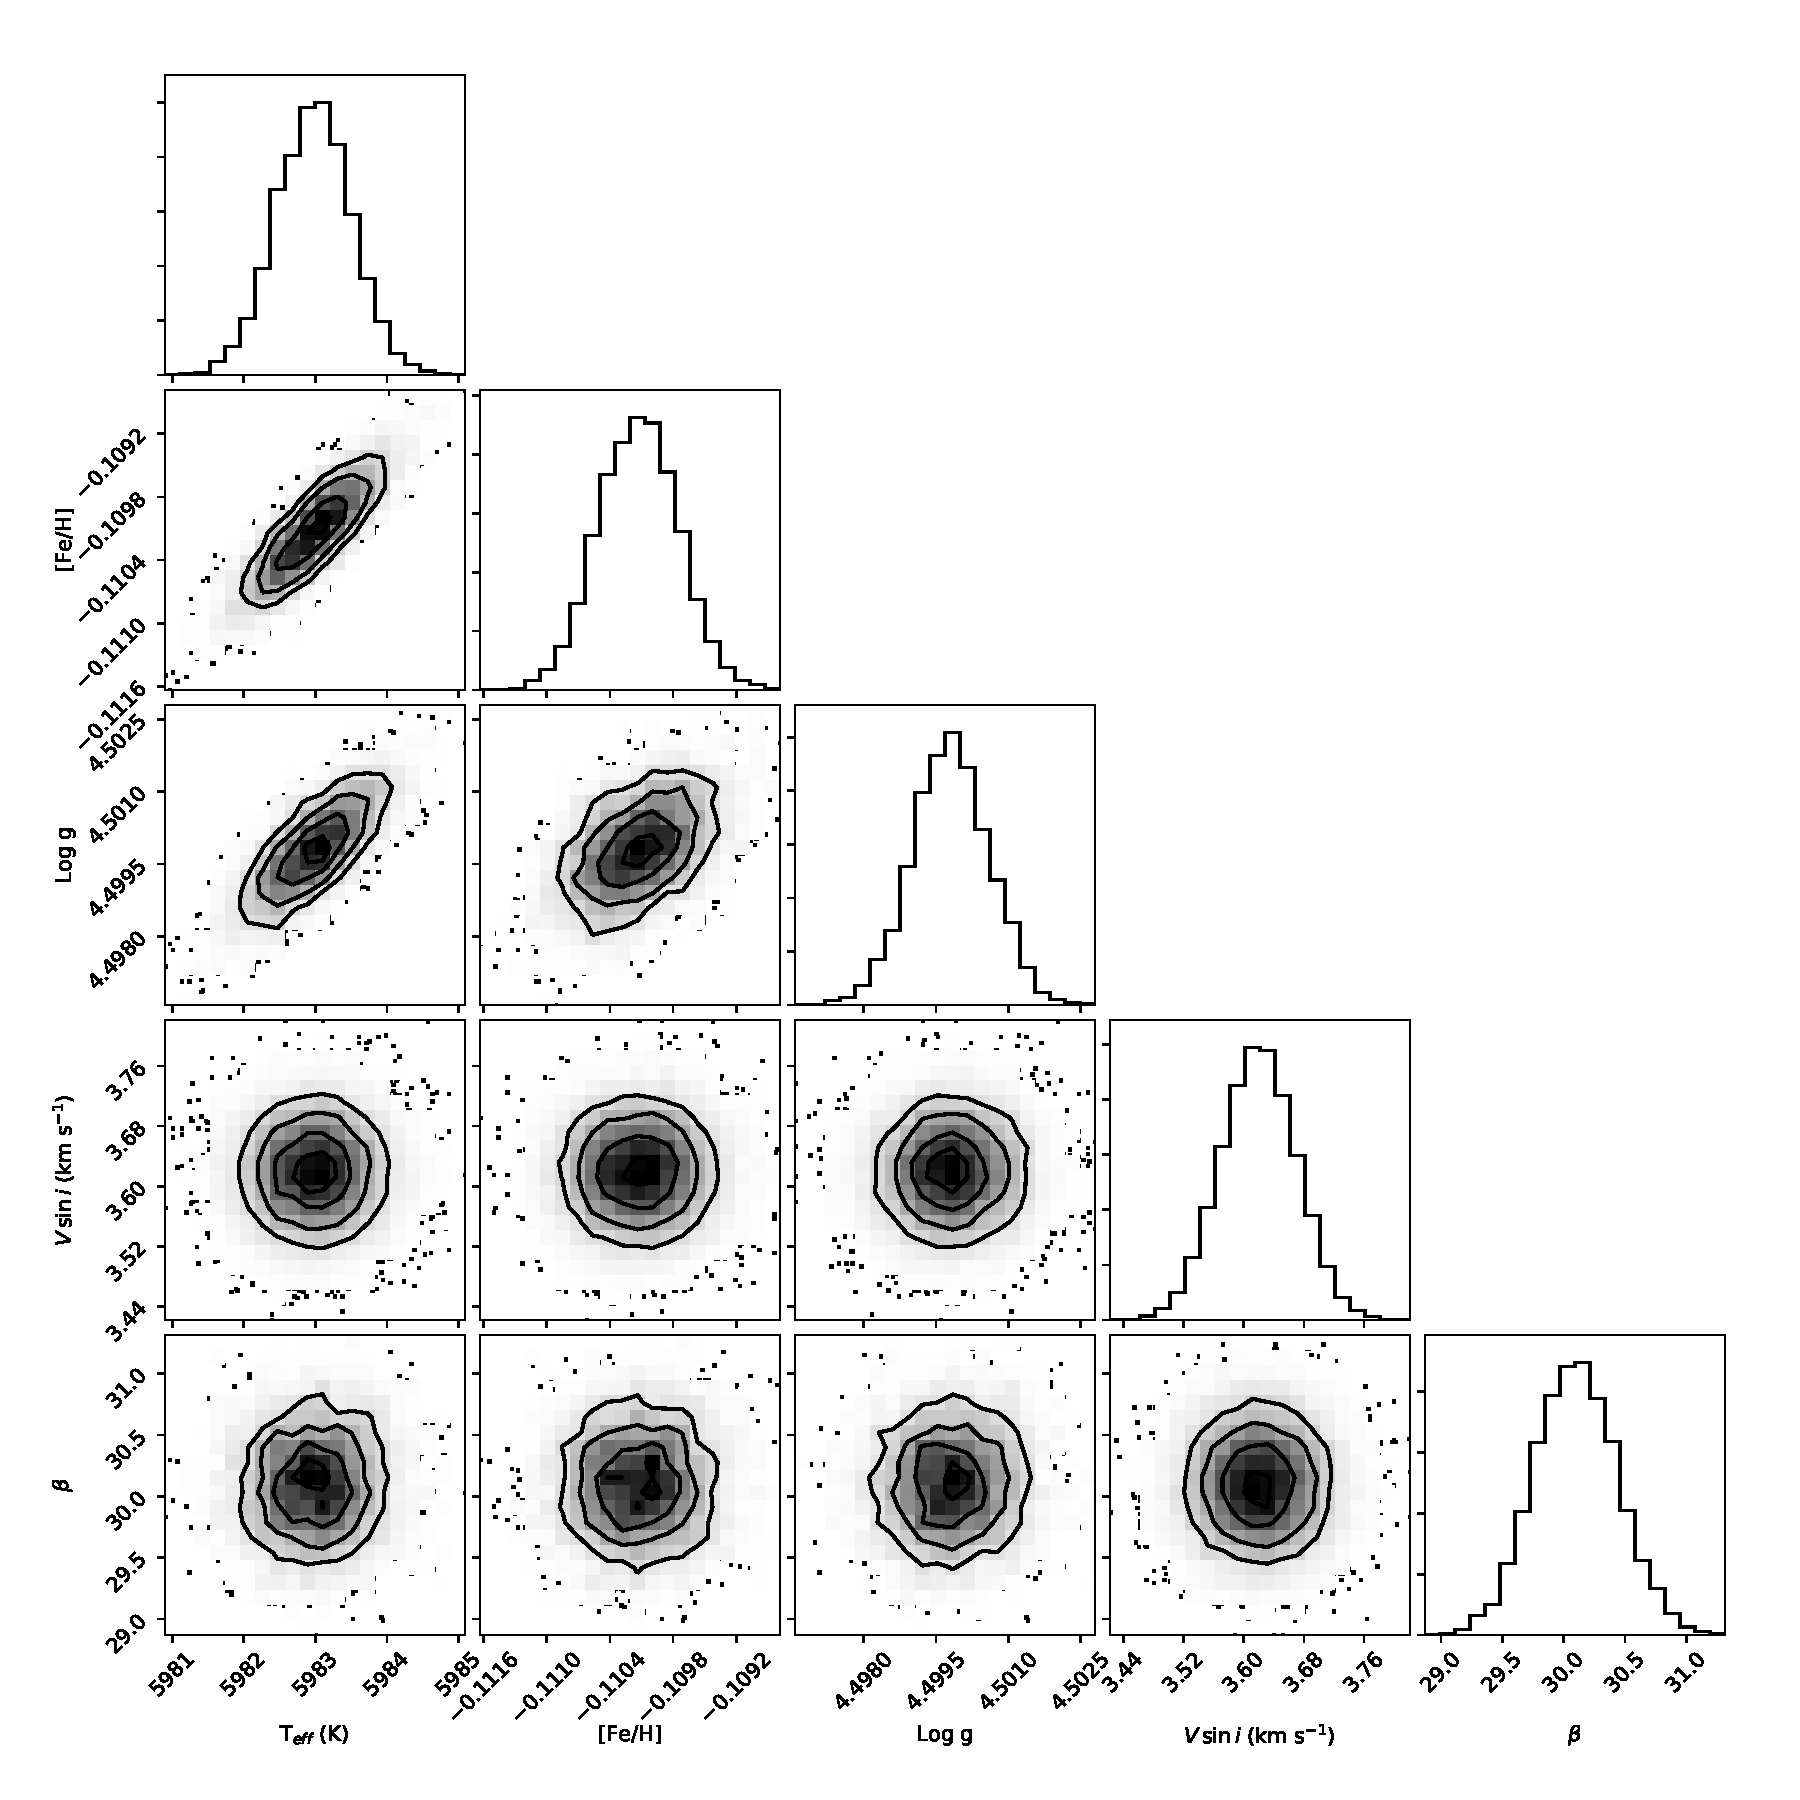
\includegraphics[width=\textwidth]{5-images/wavelet_WASP20_corner.eps}
\caption{Posterior probability distributions for WASP-20.}
\label{fig:wavelet:wavelet_corner_WASP20}
\end{figure*}





%%%%%%%%%%%%%%%%%%%%%%%%%%%%%%%%%%%%%%%%%%%%%%%%%%%%%%%%%%%%%%%%%
\section{Self consistency}\label{wavelet:self_con}
%%%%%%%%%%%%%%%%%%%%%%%%%%%%%%%%%%%%%%%%%%%%%%%%%%%%%%%%%%%%%%%%%

 \begin{figure*}
\centering
 \begin{subfigure}[b]{0.5\linewidth}
    \centering
    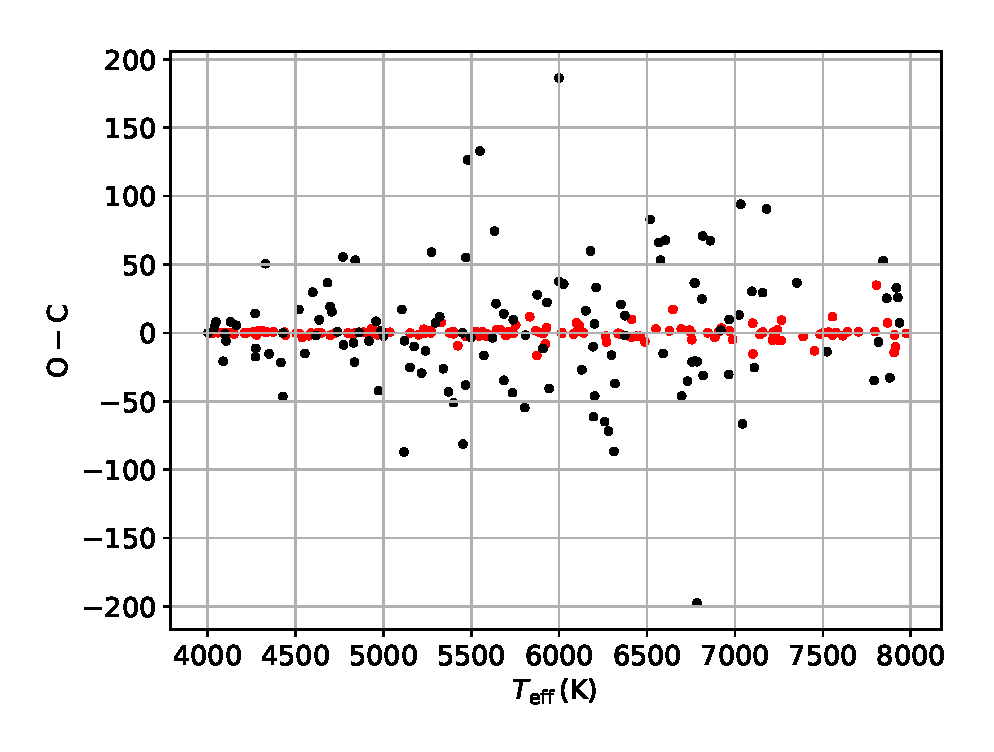
\includegraphics[width=\linewidth]{5-images/selfT.eps} 
    \label{fig7:a} 
    \vspace{4ex}
  \end{subfigure}%% 
  \begin{subfigure}[b]{0.5\linewidth}
    \centering
    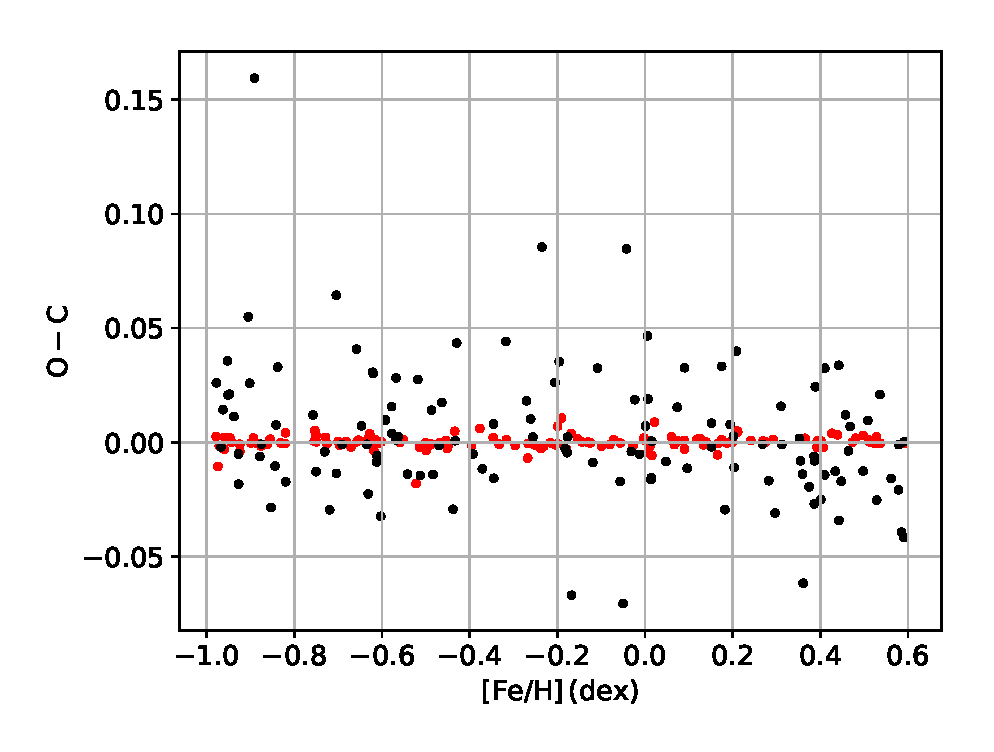
\includegraphics[width=\linewidth]{5-images/selfM.eps} 
    \label{fig7:b} 
    \vspace{4ex}
  \end{subfigure} 
  \begin{subfigure}[b]{0.5\linewidth}
    \centering
    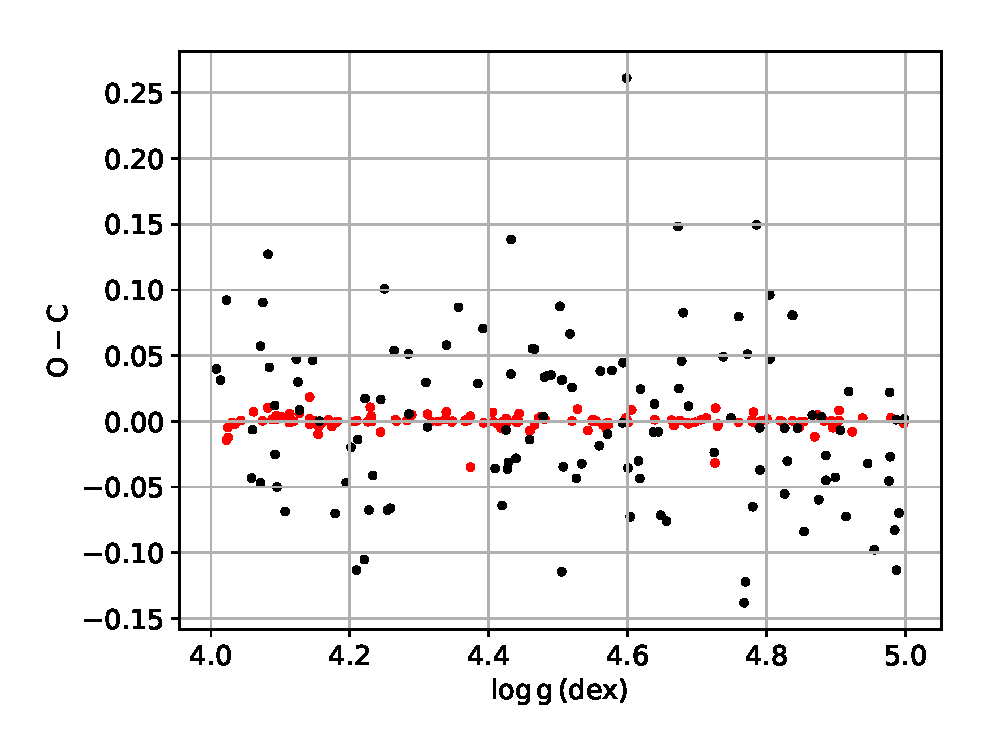
\includegraphics[width=\linewidth]{5-images/selfL.eps} 
    \label{fig7:c} 
  \end{subfigure}%%
  \begin{subfigure}[b]{0.5\linewidth}
    \centering
    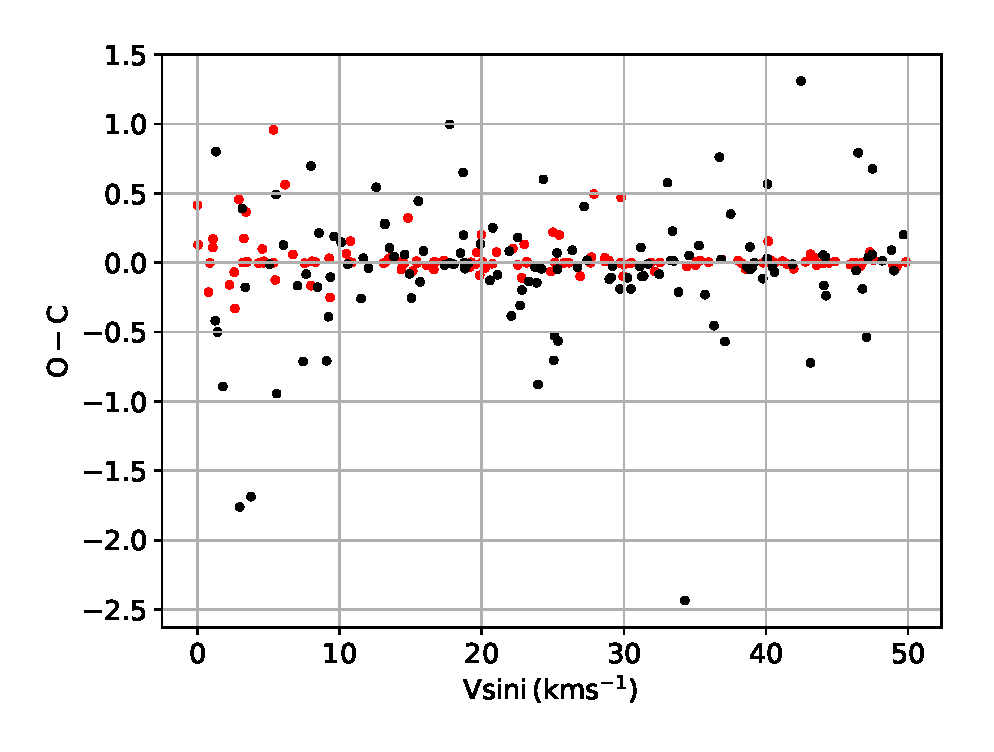
\includegraphics[width=\linewidth]{5-images/selfV.eps} 
    \label{fig7:d} 
  \end{subfigure} 
  \caption{Differences between wavelet-determined atmospheric parameters and those used to synthesise spectra with all parameters free (black) and with priors on $\log g$ (red). }

  \label{wavelet:fig:self_consistency}   
\end{figure*}


\begin{table}
\caption{The recovery of atmospheric parameters using the wavelet method for two groups of 256 spectra: one group with no priors on $\log g$ and another with priors imposed from transit photometry. The difference between the value measured by the wavelet method and the input value used to interpolate the spectrum ($\rm x_{\rm out}-\rm x_{\rm in}$) were used to calculate the standard deviation, $\sigma$, and mean offset, $\mu$.}              % title of Table
\label{wavelet:table:self_cons_tab}      % is used to refer this table in the text
\centering                                      % used for centering table
\begin{tabular}{l c r r c c c c c c}          % centered columns (4 columns)
\hline\hline                        % inserts double horizontal lines
 & \multicolumn{1}{p{2cm}}{\centering Prior on \\ $\log g$?} & $\sigma$ & $\mu$ & \\
\hline    
$T_{\rm eff}$ (K) & no & 46.0 & -3.2 \\
 & yes & 3.1  &  0.2 \\
$\rm [Fe/H]$ (dex) & no & 0.040 & -0.003 \\
 & yes & 0.020 & -0.001\\
$V \sin i$ (kms$^{-1}$) & no & 0.47 & 0.05 \\
 & yes & 0.17   & -0.06 \\
$\log g$ (dex) & no & 0.060 & -0.002\\
 & yes & 0.020 & 0.001\\

\hline                                             %inserts single line
\end{tabular}
\end{table}

I have assessed  the ability of my method to recover atmospheric parameters from synthetic spectra in order to check that my results are self consistent. I interpolated 512 spectra with random values of $T_{\rm eff}$, [Fe/H], $\log g$ and $V \sin i$ selected within the limits of my grid of models. Each spectrum was then re-sampled to have $2^{17}$ values in the range 450--650\,nm to match my choice of coefficients in Sect. \ref{wavelet:wavelet_decomposition} and the benchmark sample in Sect. \ref{wavelet:wavelet_benchmark}. These spectra were split into two groups and analysed with the aforementioned method. The first group had $\log g$ as a free parameter to probe for any systematics, for the second group I imposed a prior on $\log g$ to simulate the effect of well constrained surface gravity measurement from transit photometry. The  $\log g$ prior probability distribution was assumed to be Gaussian with a mean $\log g$ value equal to the value used to interpolate the spectrum and a dispersion equal to the average uncertainty of transit $\log g$ values from \citet{26A...558A.106M} (hereafter referred to as M13) for 44 WASP exoplanet hosts ($\overline{\sigma_{\rm \log g}}$ = 0.02 dex). I decided not to add Gaussian noise to these spectra as noise profiles depend upon stellar parameters and instrumental conditions; this is assessed  in Sect. \ref{wavelet:spec_quality}. I found typical autocorrelation lengths are below 1000 steps for all parameters in the first chain and 12 chains in the second run typically produce an acceptance fraction between $\sim\,0.25\,$ and $\,0.3$.  

The recovery of atmospheric parameters for both groups is shown in Fig.  \ref{wavelet:fig:self_consistency} and summarised in Table \ref{wavelet:table:self_cons_tab}. I found that all parameters are recovered well across the range of my grid. With no constraints on $\log g$, there were only two measurements of $T_{\rm eff}$ that deviated from the input value by more than 150\,K. A prior on $\log g$ significantly decreases the difference between measured and input atmospheric parameters and shows that my method is sensitive to $\log g$. There is a small increase in residual scatter for measurements of $V \sin i$ when the interpolated value of $V \sin i$ below 0.5\,km\,s$^{-1}$; this is seen in both groups and marginally improved with a prior on $\log g$. This is expected as the resolution of the broadening kernel in combination with the edge of parameter space makes it difficult to determine low $V \sin i$ values. The internal precision associated with the wavelet method is remarkably high; by taking $1\sigma$ values from the cumulative probability distributions I found precisions around 15\,K, 0.01\,dex, 0.02\,dex, and 0.15\,$\rm km\,s^{-1}$ for $T_{\rm eff}$, [Fe/H], $\log g$, and $V \sin i$ respectively. More realistic uncertainties are determined in the following sections. 

I also assessed the sensitivity of my method by determining the atmospheric parameters of 9 spectra from a discrete set of grid points with different combinations of fixed parameters. I interpolate 96 spectra from the following grid points -- $4800$ K, $5800$ K and $6500$ K for $T_{\rm eff}$; $-0.5$, $0.0$ and $0.5$ $dex$ for [Fe/H]; $3.75$, $4.40$ and $4.80$ $dex$ for $\log g$; $5$, $10$ and $15\,kms^{-1}$ for $V \sin i$. In total, I determined the atmospheric parameters  for each spectrum 15 times with the wavelet method using every combination of free and fixed parameters (see Fig. \ref{wavelet:fig:self_consistency_2}). I found that constraining one or more parameters increases the internal precision of the wavelet method significantly. A slight degeneracy exists between $T_{\rm eff}$ and $\log g$ resulting in a modest scatter when both parameters are left free. This also highlights the numerical noise introduced by starting walkers at different positions, since walkers explore parameter space by random jumps which may never reach the correct solution, despite prior knowledge that an exact solution lies somewhere within the grid. 

 \begin{figure*}

    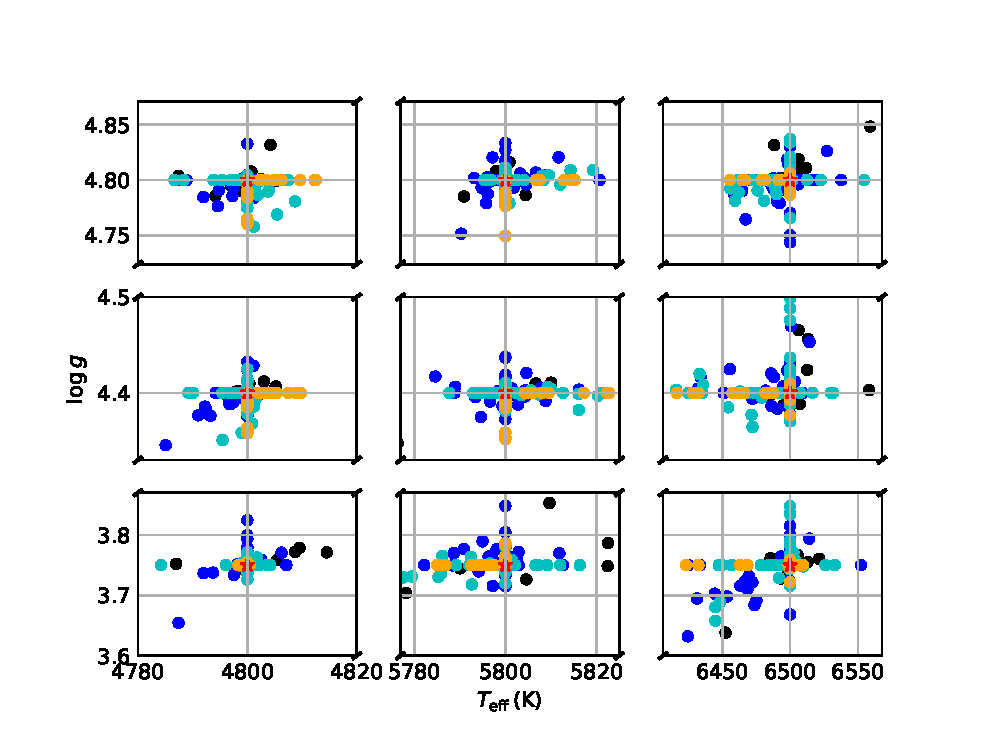
\includegraphics[scale=0.7]{5-images/self_test_2_TL.eps} 

    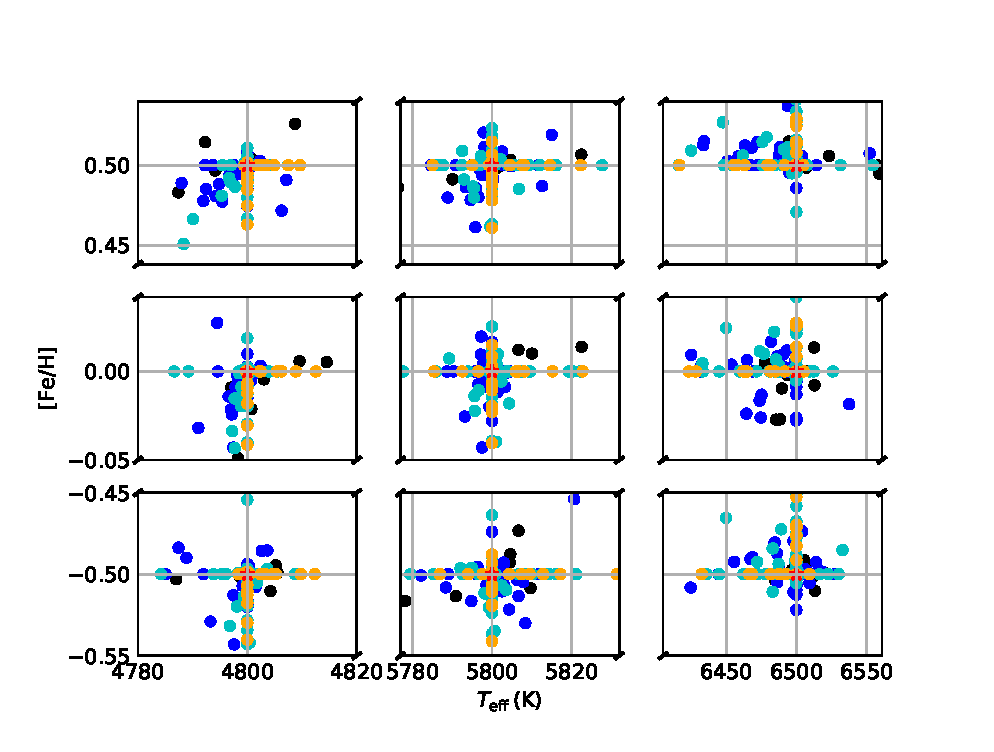
\includegraphics[scale=0.7]{5-images/self_test_2_TM.eps} 

  \caption{Difference between atmospheric parameters determined by the wavelet method for 9 synthetic spectra when some parameters are fixed. I plot atmospheric parameters determined with with all parameters free ($T_{\rm eff}$, [Fe/H], $\log g$, $V \sin i$) in black; with one parameter fixed in blue; with two parameters fixed in cyan; three parameters fixed in orange.  }
  \label{wavelet:fig:self_consistency_2}   
\end{figure*}



\section{Benchmark sample}\label{wavelet:wavelet_benchmark}


\begin{table}[ht!]
\caption{My benchmark sample of FGK stars from D15. I include the V magnitude, the number of spectra and the S/N of the coadded spectra at 500\,nm.}              % title of Table
\label{WASP_STARS}      % is used to refer this table in the text
\centering                                      % used for centering table
\begin{tabular}{l r r r r}          % centered columns (4 columns)
\hline\hline                        % inserts double horizontal lines
 Star & V mag & \multicolumn{1}{p{2cm}}{\centering \# of \\ spectra} & \multicolumn{1}{p{2cm}}{\centering SNR\\ ($\sim$500 nm)} \\
\hline    
WASP-4  & 12.50 & 12 & 37 \\
WASP-5  & 12.30 & 11 & 35 \\
WASP-6  & 11.90 & 30 & 63 \\
WASP-7  &  9.50 & 13 & 124 \\
WASP-8  &  9.79 & 21 & 137 \\
WASP-15 & 11.00 & 15 & 83\\
WASP-16 & 11.30 & 19 & 77\\
WASP-17 & 11.60 & 42 & 71\\
WASP-18 &  9.30 &  5 & 119 \\
WASP-19 & 12.59 & 28 & 50\\
WASP-20 & 10.68 & 58 & 153 \\
WASP-22 & 12.00 & 29 & 63\\
WASP-23 & 12.68 & 38 & 53\\
WASP-24 & 11.31 & 18 & 53\\
WASP-29 & 11.30 & 14 & 57\\
WASP-30 & 11.90 & 47 & 27\\
WASP-31 & 11.70 & 35 & 53\\
WASP-53 & 12.19  & 35 & 40\\
WASP-69 &  9.88 & 21 & 136 \\
WASP-80 & 11.90 & 37 & 51\\
\hline                                             %inserts single line
\end{tabular}
\end{table}



Any spectral analysis technique must be tested against stars with high-quality measurements. For this  I use stars from  \citet{Doyle2013} and (\citealt{Doyle2015}; D15, hereafter). The D15 sample consists of 24 stars analysed by measurements of EW and spectral fitting of high-S/N and high-resolution ($\rm R\,=\,112,000$) data from the HARPS spectrograph \citep{2001Msngr.105....1Q}. I used lower-quality observations from the CORALIE spectrograph to determine $T_{\rm eff}$, [Fe/H], $\log g$ and $V \sin i$ of the same stars with the wavelet method. Only 22 stars in the D15 sample have CORALIE spectra available to use and I further exclude WASP-77A and the close (3") B-component as both component as they are un-resolved in the CORALIE fibre. This leaves a sample of 20 stars for use to calibrate my method (see Table \ref{WASP_STARS}).



\section{CORALIE spectra}\label{CORALIE_data}

Each spectrum was processed with the CORALIE standard data-reduction pipeline \citep{26AS..119..373B}. The radial velocity shift was measured relative to a solar template\footnote{From The Gaia Benchmark Stars Library pipeline which is the result of co-adding asteroid observations by NARVAL.} and corrected into a laboratory frame of reference. The spectra were then median-combined onto an identically sampled wavelength grid. Continuum regions were identified by applying maximum and median filters  \citep{Blanco-Cuaresma2017} and fitted with spline functions (1 every 10\,nm) for normalisation. The wavelet method was then applied to each spectrum twice: once with no priors on $\log g$ and a second time with priors given by transit photometry. The priors on $\log g$ were set to those from M13 if quoted, or the relevant discovery papers otherwise (see Table \ref{wavelet:table:doyle_tab}).  




\section{Results}\label{D15_results}

 \begin{figure*}
\centering
 \begin{subfigure}[b]{0.5\linewidth}
    \centering
    \includegraphics[width=\linewidth]{5-images/doyleT} 
    \caption{} 
    \label{doyle:a} 
    \vspace{4ex}
  \end{subfigure}%% 
  \begin{subfigure}[b]{0.5\linewidth}
    \centering
    \includegraphics[width=\linewidth]{5-images/doyleM} 
    \caption{} 
    \label{doyle:b} 
    \vspace{4ex}
  \end{subfigure} 
  \begin{subfigure}[b]{0.5\linewidth}
    \centering
    \includegraphics[width=\linewidth]{5-images/doyleL} 
    \caption{} 
    \label{doyle:c} 
  \end{subfigure}%%
  \begin{subfigure}[b]{0.5\linewidth}
    \centering
   \includegraphics[width=\linewidth]{5-images/doyleV} 
    \caption{} 
    \label{doyle:d} 
  \end{subfigure} 
  \caption{Difference between wavelet analysis and D15 (O-C) for each atmospheric parameter in the D15 sample. Each spectrum was measured twice, once with $\log g$ as a free parameter (black) and again with $\log g$ priors imposed from transit photometry (red).  I exclude measurements of $V \sin i$ where macroturbulence, $\xi_t$, was set to $0\,\rm km\,s^{-1}$ to ensure models a best model was converged upon.}
  \label{wavelet:fig:doyle}   
\end{figure*}



\begin{table}
\caption{Recovery of atmospheric parameters for 20 FGK stars from D15: one group with no priors on $\log g$ and another with priors from transit photometry. The difference between the value measured by the wavelet method and D15 ($x_{wavelet}-x_{D15}$) are used to calculate the mean dispertion, $\sigma$, and mean offset $\mu$.}              % title of Table
\label{wavelet:table:doyle_tab}      % is used to refer this table in the text
\centering                                      % used for centering table
\begin{tabular}{l l r r c c }          % centered columns (4 columns)
\hline\hline                        % inserts double horizontal lines
 & \multicolumn{1}{p{2cm}}{\centering Prior on \\ $\log g$?} & $\sigma$ & $\mu$ & \\
\hline    
$T_{\rm eff}$ (K) & no & 85.00 &  31.00 \\
 & yes & 86.00  &  14.00 \\
$\rm [Fe/H]$ (dex) & no & 0.06 & $-$ 0.15 \\
 & yes & 0.10 & $-$ 0.18 \\
$V \sin i$ (kms$^{-1}$) & no & 1.35  & $-$ 0.79 \\
 & yes & 0.62 &  $-$ 1.33 \\
$\log g$ (dex) & no & 0.13 & 0.08 \\
 & yes & 0.14 &  0.05 \\\\\hline                                             %inserts single line
\end{tabular}
\tablefoot{Values of $\sigma$ and $\mu$ for $V \sin i$ excluded stars where macroturbulence, $\xi_t$, was set to $\rm 0\, \rm km\,s^{-1}$.}
\end{table}


% Include the main table of results
\begin{sidewaystable*}[t!]
\caption{Descriptions of 20 WASP targets used for this work.}              
\centering
\resizebox{\linewidth}{!}{%
\begin{tabular}{l r r r r r r r r r r r r r r}     % 7 columns 
\hline\hline   
                      % To combine 4 columns into a single one 
%Star & \multicolumn{1}{p{2cm}}{\centering $SNR$ \\ (at 500$nm$)} & \multicolumn{1}{p{2cm}}{\centering $T_{eff}$ \\ (K) \\ \protect\cite{Doyle2015}} & \multicolumn{1}{p{2cm}}{\centering $T_{eff}$ \\ (K) \\This Work}\\
                  
 %  4  & 34.4 & \multicolumn{1}{p{2cm}}{\centering 5400 \\$\pm$ 90} & \multicolumn{1}{p{2cm}}{\centering 5432 \\ $\pm$ 80}\\ 
%   5  & 32.9 & \multicolumn{1}{p{2cm}}{\centering 5690 \\$\pm$ 80} & \multicolumn{1}{p{2cm}}{\centering 5715 \\ $\pm$ 80}\\ 

Star & 
\multicolumn{1}{p{2cm}}{\centering $T_{eff}$ \\ (K) \\ This Work} & 
\multicolumn{1}{p{2cm}}{\centering $T_{eff}$ \\ (K) \\ $log g$ prior}  & 
\multicolumn{1}{p{2cm}}{\centering $T_{eff}$ \\ (K) \\ D15} & 
\multicolumn{1}{p{2cm}}{\centering $Log$ $g$\\ (c.g.s) \\ This Work}  & 
\multicolumn{1}{p{2cm}}{\centering $Log$ $g$\\ (c.g.s)\\ D15} & 
\multicolumn{1}{p{2cm}}{\centering $Log$ $g$\\ (c.g.s)\\ photometry}  & 
\multicolumn{1}{p{2cm}}{\centering $[Fe/H]$ \\ (dex) \\ This Work}  & 
\multicolumn{1}{p{2cm}}{\centering $[Fe/H]$ \\ (dex) \\ $log g$ prior} & 
\multicolumn{1}{p{2cm}}{\centering $[Fe/H]$ \\ (dex)\\ D15} & 
\multicolumn{1}{p{2cm}}{\centering $V.sini$ \\ $kms^{-1}$ \\ This Work} & 
\multicolumn{1}{p{2cm}}{\centering $V.sini$ \\ $kms^{-1}$ \\ $log g$ prior} & \multicolumn{1}{p{2cm}}{\centering $V.sini$ \\ $kms^{-1}$ \\ D15}  \\
%& \multicolumn{1}{p{2cm}}{\centering SNR \\ at 500$nm$} \\
\hline  
% 4   & 5432 & 80 & 5400 & 90  & 4.58  & 0.1 & 4.47 & 0.11  & -0.18  & 0.07 & -0.1  & 0.1  & 0.92  & 0.8 & 3.4  & 0.3  & 12.5  & 34.4   \\ 
 %done  
 
 
 WASP-4 *
& 5524 $\pm$ 11
& 5549 $\pm$ 10 
& 5400 $\pm$ 90
& 4.5  $\pm$ 0.02
& 4.47  $\pm$ 0.11
&  4.49 $\pm$ 0.01 $^1$
& -0.08  $\pm$ 0.01
& -0.04  $\pm$ 0.01 
&-0.1 $\pm$ 0.1 
& 4.62  $\pm$ 0.11 
& 4.92  $\pm$ 0.11 
& 3.40 $\pm$ 0.30 \\
%&  34.4 & 12.5\\
                     
%WASP-4 *
%& \multicolumn{1}{p{2cm}}{\centering 5524 \\ $\pm$ 11} 
%& \multicolumn{1}{p{2cm}}{\centering 5549 \\$\pm$ 10} &
%\multicolumn{1}{p{2cm}}{\centering 5400 \\$\pm$ 90} 
%& \multicolumn{1}{p{2cm}}{\centering 4.5 \\ $\pm$ 0.02}  
%& \multicolumn{1}{p{2cm}}{\centering 4.47 \\ $\pm$ 0.11} 
%& \multicolumn{1}{p{2cm}}{\centering 4.49 \\ $\pm$ 0.01 $^1$} 
%& \multicolumn{1}{p{2cm}}{\centering -0.08 \\ $\pm$ 0.01} &
%multicolumn{1}{p{2cm}}{\centering -0.04 \\ $\pm$ 0.01} 
%&\multicolumn{1}{p{2cm}}{\centering -0.1 \\ $\pm$ 0.1} 
%& \multicolumn{1}{p{2cm}}{\centering 4.62 \\ $\pm$ 0.11} 
%&\multicolumn{1}{p{2cm}}{\centering 4.92 \\ $\pm$ 0.11} 
%& \multicolumn{1}{p{2cm}}{\centering 3.40 \\ $\pm$ 0.30} \\
%&  34.4 & 12.5\\



%done
%5     & 5715 & 80 & 5690 & 80  & 4.50  & 0.1 & 4.28 & 0.9   & 0.0    & 0.07 & 0.11  & 0.1  & 2.62  & 0.8 & 3.9  & 0.2  & 12.3  & 32.9   \\ 

WASP-5  
& 5806  $\pm$ 17
&  5617  $\pm$ 16
&  5690 $\pm$ 80
& 4.58  $\pm$ 0.01
&  4.28  $\pm$ 0.9
&  4.39  $\pm$ 0.03 $^1$ 
&  0.0  $\pm$ 0.01 
& -0.09  $\pm$ 0.01
&  0.11  $\pm$ 0.1
&  2.62  $\pm$ 0.12
&  $\leq$0.5  $\pm$ 0.14
&  3.90  $\pm$ 0.2 \\



%WASP-5  & \multicolumn{1}{p{2cm}}{\centering 5806 \\ $\pm$ 17} 
%&
%\multicolumn{1}{p{2cm}}{\centering 5617 \\ $\pm$ 16} 
%& \multicolumn{1}{p{2cm}}{\centering 5690 \\$\pm$ 80} 
%& \multicolumn{1}{p{2cm}}{\centering 4.58 \\ $\pm$ 0.01}  
%& \multicolumn{1}{p{2cm}}{\centering 4.28 \\ $\pm$ 0.9} 
%& \multicolumn{1}{p{2cm}}{\centering 4.39 \\ $\pm$ 0.03 $^1$} 
%& \multicolumn{1}{p{2cm}}{\centering 0.0 \\ $\pm$ 0.01} 
%\multicolumn{1}{p{2cm}}{\centering -0.09 \\ $\pm$ 0.01} 
%& \multicolumn{1}{p{2cm}}{\centering 0.11 \\ $\pm$ 0.1} 
%& \multicolumn{1}{p{2cm}}{\centering 2.62 \\ $\pm$ 0.12} 
%&\multicolumn{1}{p{2cm}}{\centering $\leq$0.5 \\ $\pm$ 0.14} 
%& \multicolumn{1}{p{2cm}}{\centering 3.90 \\ $\pm$ 0.2} \\

%6     & 5347 & 80 & 5375 & 65  & 4.56  & 0.1 & 4.61 & 0.07  & -0.36  & 0.07 %& -0.17 & 0.09 & 3.22  & 0.8 & 2.4  & 0.5  & 11.9  & 59.9  \\ 
%done
WASP-6  
& 5380  $\pm$ 15
& 5427  $\pm$ 19
& 5375 $\pm$ 65
&  4.57  $\pm$ 0.01  
&  4.61  $\pm$ 0.07  
&  4.52  $\pm$ 0.01 $^1$
&  -0.35  $\pm$ 0.01 
& -0.32  $\pm$ 0.01
&  -0.17  $\pm$ 0.09
&  2.95  $\pm$ 0.21
& 3.01   $\pm$ 0.19
&  2.40  $\pm$ 0.5 \\

%WASP-6  & \multicolumn{1}{p{2cm}}{\centering 5380 \\ $\pm$ 15} 
%&\multicolumn{1}{p{2cm}}{\centering 5427 \\ $\pm$ 19} 
%& \multicolumn{1}{p{2cm}}{\centering 5375 \\$\pm$ 65} 
%& \multicolumn{1}{p{2cm}}{\centering 4.57 \\ $\pm$ 0.01}  
%& \multicolumn{1}{p{2cm}}{\centering 4.61 \\ $\pm$ 0.07}  
%& \multicolumn{1}{p{2cm}}{\centering 4.52 \\ $\pm$ 0.01 $^1$} 
%& \multicolumn{1}{p{2cm}}{\centering -0.35 \\ $\pm$ 0.01} 
%&\multicolumn{1}{p{2cm}}{\centering -0.32 \\ $\pm$ 0.01} 
%& \multicolumn{1}{p{2cm}}{\centering -0.17 \\ $\pm$ 0.09} 
%& \multicolumn{1}{p{2cm}}{\centering 2.95 \\ $\pm$ 0.21} 
%&\multicolumn{1}{p{2cm}}{\centering 3.01  \\ $\pm$ 0.19} 
%& \multicolumn{1}{p{2cm}}{\centering 2.40 \\ $\pm$ 0.5} \\

%7     & 6538 & 80 & 6550 & 70  & 4.43  & 0.1 & 4.32 & 0.06  & -0.021 & 0.07 & 0.16  & 0.06 & 17.32 & 0.8 & 18.1 & 0.02 & 9.5   & 144    \\
% done
WASP-7  
&  6532  $\pm$ 10
& 6494  $\pm$ 9
&  6550 $\pm$ 70
&  4.41  $\pm$ 0.2
&  4.32  $\pm$ 0.07
&  4.22  $\pm$ 0.04 $^1$
&  0.0  $\pm$ 0.01
& -0.01  $\pm$ 0.01
&  0.16  $\pm$ 0.06
& 17.14  $\pm$ 0.15
& 17.27  $\pm$ 0.14
&  18.10   $\pm$ 0.02 \\

%WASP-7  & \multicolumn{1}{p{2cm}}{\centering 6532 \\ $\pm$ 10} 
%&\multicolumn{1}{p{2cm}}{\centering 6494 \\ $\pm$ 9} 
%& \multicolumn{1}{p{2cm}}{\centering 6550 \\$\pm$ 70} 
%& \multicolumn{1}{p{2cm}}{\centering 4.41 \\ $\pm$ 0.2}  
%& \multicolumn{1}{p{2cm}}{\centering 4.32 \\ $\pm$ 0.07} 
%& \multicolumn{1}{p{2cm}}{\centering 4.22 \\ $\pm$ 0.04 $^1$}
%& \multicolumn{1}{p{2cm}}{\centering 0.0 \\ $\pm$ 0.01} 
%&\multicolumn{1}{p{2cm}}{\centering -0.01 \\ $\pm$ 0.01} 
%& \multicolumn{1}{p{2cm}}{\centering 0.16 \\ $\pm$ 0.06} 
%& \multicolumn{1}{p{2cm}}{\centering 17.14 \\ $\pm$ 0.15} 
%&\multicolumn{1}{p{2cm}}{\centering 17.27 \\ $\pm$ 0.14} 
%& \multicolumn{1}{p{2cm}}{\centering 18.10  \\ $\pm$ 0.02}\\
 
%8     & 5525 & 80 & 5560 & 90  & 4.47  & 0.1 & 4.4  & 0.09  & 0.012  & 0.07 & 0.18  & 0.11 & 0.217 & 0.8 & 2.7  & 0.5  & 9.79  & 206.7 \\
% done
WASP-8* 
&  5578  $\pm$ 15 
& 5488  $\pm$ 9 
&  5560 $\pm$ 90 
&   4.56  $\pm$ 0.01  
&  4.40  $\pm$ 0.09 
& 4.48  $\pm$ 0.01 $^1$
&  0.09  $\pm$ 0.01
& 0.03  $\pm$ 0.01
&  0.18   $\pm$ 0.11
&  $\leq$ 0.50  $\pm$ 0.17 
& $\leq$ 0.50  $\pm$ 0.17
&  2.70   $\pm$ 0.50  \\

%WASP-8* & \multicolumn{1}{p{2cm}}{\centering 5578 \\ $\pm$ 15} 
%&\multicolumn{1}{p{2cm}}{\centering 5488 \\ $\pm$ 9} 
%& \multicolumn{1}{p{2cm}}{\centering 5560 \\$\pm$ 90} 
%& \multicolumn{1}{p{2cm}}{\centering  4.56 \\ $\pm$ 0.01}  
%& \multicolumn{1}{p{2cm}}{\centering 4.40 \\ $\pm$ 0.09} 
%& \multicolumn{1}{p{2cm}}{\centering 4.48 \\ $\pm$ 0.01 $^1$}
%& \multicolumn{1}{p{2cm}}{\centering 0.09 \\ $\pm$ 0.01}
%&\multicolumn{1}{p{2cm}}{\centering 0.03 \\ $\pm$ 0.01} 
%& \multicolumn{1}{p{2cm}}{\centering 0.18  \\ $\pm$ 0.11} 
%& \multicolumn{1}{p{2cm}}{\centering $\leq$ 0.50 \\ $\pm$ 0.17} 
%&\multicolumn{1}{p{2cm}}{\centering $\leq$ 0.50 \\ $\pm$ 0.17} 
%& \multicolumn{1}{p{2cm}}{\centering 2.70  \\ $\pm$ 0.50}  \\

%15    & 6455 & 80 & 6405 & 80  & 4.469 & 0.1 & 4.4  & 0.11  & -0.129 & 0.07 & 0     & 0.1  & 3.36  & 0.8 & 4.9  & 0.4  & 11    & 110.3  \\ 
% done
%WASP-15*  & \multicolumn{1}{p{2cm}}{\centering 6428 \\ $\pm$ 14} 
%&\multicolumn{1}{p{2cm}}{\centering 6395 \\ $\pm$ 14} 
%& \multicolumn{1}{p{2cm}}{\centering 6405 \\$\pm$ 80} 
%& \multicolumn{1}{p{2cm}}{\centering  4.44 \\ $\pm$ 0.01}  
%& \multicolumn{1}{p{2cm}}{\centering 4.40 \\ $\pm$ 0.11} 
%& \multicolumn{1}{p{2cm}}{\centering 4.22 \\ $\pm$ 0.02 $^1$}
%& \multicolumn{1}{p{2cm}}{\centering -0.16 \\ $\pm$ 0.01} 
%&\multicolumn{1}{p{2cm}}{\centering 0.03 \\ $\pm$ 0.01} 
%& \multicolumn{1}{p{2cm}}{\centering 0.00  \\ $\pm$ 0.10} 
%& \multicolumn{1}{p{2cm}}{\centering 5.47 \\ $\pm$ 0.19} 
%&\multicolumn{1}{p{2cm}}{\centering 5.38 \\ $\pm$ 0.11} 
%& \multicolumn{1}{p{2cm}}{\centering 4.90  \\ $\pm$ 0.40} \\

WASP-15*  
&  6428  $\pm$ 14 
& 6395  $\pm$ 14 
&  6405 $\pm$ 8
&   4.44  $\pm$ 0.01  
&  4.40  $\pm$ 0.11 
&  4.22  $\pm$ 0.02 $^1$
&  -0.16  $\pm$ 0.01
& 0.03  $\pm$ 0.01 
&  0.00   $\pm$ 0.10
&  5.47  $\pm$ 0.19 
& 5.38  $\pm$ 0.11 
&  4.90   $\pm$ 0.40 \\

%16    & 5670 & 80 & 5550 & 60  & 4.43  & 0.1 & 4.21 & 0.011 & -0.08  & 0.07 & 0.07  & 0.1  & 1.68  & 0.8 & 2.5  & 0.4  & 11.3  & 94.22  \\ 
% done
%WASP-16*  & \multicolumn{1}{p{2cm}}{\centering 5735 \\ $\pm$ 14} 
%&\multicolumn{1}{p{2cm}}{\centering 5561 \\ $\pm$ 13} 
%& \multicolumn{1}{p{2cm}}{\centering 5550 \\$\pm$ 60} 
%& \multicolumn{1}{p{2cm}}{\centering  4.48 \\ $\pm$ 0.03}  
%& \multicolumn{1}{p{2cm}}{\centering 4.21 \\ $\pm$ 0.01} 
%& \multicolumn{1}{p{2cm}}{\centering 4.49 \\ $\pm$ 0.02 $^1$}
%& \multicolumn{1}{p{2cm}}{\centering -0.02 \\ $\pm$ 0.01} 
%&\multicolumn{1}{p{2cm}}{\centering -0.14 \\ $\pm$ 0.01} 
%& \multicolumn{1}{p{2cm}}{\centering 0.07  \\ $\pm$ 0.10} 
%& \multicolumn{1}{p{2cm}}{\centering 1.30 \\ $\pm$ 0.21} 
%&\multicolumn{1}{p{2cm}}{\centering 1.40 \\ $\pm$ 0.20} 
%& \multicolumn{1}{p{2cm}}{\centering 2.50  \\ $\pm$ 0.40}  \\

WASP-16*  
& 5735  $\pm$ 14 
& 5561  $\pm$ 13 
&  5550 $\pm$ 60 
&   4.48  $\pm$ 0.03  
&  4.21  $\pm$ 0.01 
&  4.49  $\pm$ 0.02 $^1$
&  -0.02  $\pm$ 0.01 
& -0.14  $\pm$ 0.01 
&  0.07   $\pm$ 0.10 
& 1.30  $\pm$ 0.21 
& 1.40  $\pm$ 0.20 
& 2.50   $\pm$ 0.40  \\

%17     
% done
%WASP-17  & \multicolumn{1}{p{2cm}}{\centering 6699 \\ $\pm$ 15} 
%&\multicolumn{1}{p{2cm}}{\centering 6753 \\ $\pm$ 15} 
%& \multicolumn{1}{p{2cm}}{\centering 6700 \\$\pm$ 105} 
%& \multicolumn{1}{p{2cm}}{\centering  4.27 \\ $\pm$ 0.01} 
% & \multicolumn{1}{p{2cm}}{\centering 4.34 \\ $\pm$ 0.23} 
% & \multicolumn{1}{p{2cm}}{\centering 4.16 \\ $\pm$ 0.02 $^1$}
% & \multicolumn{1}{p{2cm}}{\centering -0.24 \\ $\pm$ 0.01} 
% &\multicolumn{1}{p{2cm}}{\centering -0.22 \\ $\pm$ 0.01} 
% & \multicolumn{1}{p{2cm}}{\centering -0.12  \\ $\pm$ 0.10} 
% & \multicolumn{1}{p{2cm}}{\centering 7.86 \\ $\pm$ 0.22} 
 %&\multicolumn{1}{p{2cm}}{\centering 7.59 \\ $\pm$ 0.22} 
 %& \multicolumn{1}{p{2cm}}{\centering 9.80  \\ $\pm$ 1.10} \\
 
 WASP-17  
 & 6699  $\pm$ 15 
& 6753  $\pm$ 15 
&  6700 $\pm$ 105 
&   4.27  $\pm$ 0.01 
 &  4.34  $\pm$ 0.23 
 &  4.16  $\pm$ 0.02 $^1$
 &  -0.24  $\pm$ 0.01 
 & -0.22  $\pm$ 0.01 
 &  -0.12   $\pm$ 0.10
 &  7.86  $\pm$ 0.22 
 & 7.59  $\pm$ 0.22 
 &  9.80  $\pm$ 1.10 \\

%18    & 6420 & 80 & 6400 & 75  & 4.468 & 0.1 & 4.32 & 0.09  & -0.047 & 0.07 & 0.08  & 0.08 & 10.25 & 0.8 & 10.9 & 0.7  & 9.3   & 164.4  \\
% done
%WASP-18  & \multicolumn{1}{p{2cm}}{\centering 6434 \\ $\pm$ 13} 
%&\multicolumn{1}{p{2cm}}{\centering 6354 \\ $\pm$ 15} 
%& \multicolumn{1}{p{2cm}}{\centering 6400 \\$\pm$ 75} 
%& \multicolumn{1}{p{2cm}}{\centering  4.47 \\ $\pm$ 0.02}  
%& \multicolumn{1}{p{2cm}}{\centering 4.32 \\ $\pm$ 0.09} 
%& \multicolumn{1}{p{2cm}}{\centering 4.32 \\ $\pm$ 0.03 $^1$}
%& \multicolumn{1}{p{2cm}}{\centering -0.04 \\ $\pm$ 0.01} 
%&\multicolumn{1}{p{2cm}}{\centering -0.09 \\ $\pm$ 0.01} 
%& \multicolumn{1}{p{2cm}}{\centering 0.08  \\ $\pm$ 0.08} 
%& \multicolumn{1}{p{2cm}}{\centering 10.11 \\ $\pm$ 0.17} 
%&\multicolumn{1}{p{2cm}}{\centering 9.95 \\ $\pm$ 0.13} 
%& \multicolumn{1}{p{2cm}}{\centering 10.9  \\ $\pm$ 0.7} \\


WASP-18  
&  6434  $\pm$ 13 
& 6354  $\pm$ 15 
&  6400 $\pm$ 75 
&   4.47  $\pm$ 0.02 
&  4.32  $\pm$ 0.09 
& 4.32  $\pm$ 0.03 $^1$
&  -0.04  $\pm$ 0.01 
& -0.09  $\pm$ 0.01
&  0.08   $\pm$ 0.08 
&  10.11  $\pm$ 0.17 
& 9.95  $\pm$ 0.13 
&  10.9   $\pm$ 0.7 \\
 
%19    & 5484 & 80 & 5460 & 90  & 4.50  & 0.1 & 4.37 & 0.14  & -0.02  & 0.07 & 0.14  & 0.11 & 5.04  & 0.8 & 5.1  & 0.3  & 12.59 & 53.6  \\ 
%done
%WASP-19  & \multicolumn{1}{p{2cm}}{\centering 5573 \\ $\pm$ 17} 
%&\multicolumn{1}{p{2cm}}{\centering 5540 \\ $\pm$ 16} 
%& \multicolumn{1}{p{2cm}}{\centering 5460 \\$\pm$ 90} 
%& \multicolumn{1}{p{2cm}}{\centering  4.51 \\ $\pm$ 0.02}  
%& \multicolumn{1}{p{2cm}}{\centering 4.37 \\ $\pm$ 0.14} 
%& \multicolumn{1}{p{2cm}}{\centering 4.44 \\ $\pm$ 0.01 $^1$}
%& \multicolumn{1}{p{2cm}}{\centering 0.02 \\ $\pm$ 0.01} 
%&\multicolumn{1}{p{2cm}}{\centering 0.02 \\ $\pm$ 0.01} 
%& \multicolumn{1}{p{2cm}}{\centering 0.14  \\ $\pm$ 0.11} 
%& \multicolumn{1}{p{2cm}}{\centering 3.75 \\ $\pm$ 0.13} 
%&\multicolumn{1}{p{2cm}}{\centering 3.71 \\ $\pm$ 0.13} 
%& \multicolumn{1}{p{2cm}}{\centering 5.1  \\ $\pm$ 0.3}   \\

WASP-19  
&  5573  $\pm$ 17 
& 5540  $\pm$ 16
&  5460 $\pm$ 90 
&   4.51  $\pm$ 0.02  
&  4.37  $\pm$ 0.14 
&  4.44  $\pm$ 0.01 $^1$
&  0.02  $\pm$ 0.01 
& 0.02  $\pm$ 0.01 
&  0.14   $\pm$ 0.11 
&  3.75  $\pm$ 0.13 
& 3.71  $\pm$ 0.13 
&  5.1   $\pm$ 0.3   \\


%20    & 5983 & 80 & 6030 & 80  & 4.50  & 0.1 & 4.54 & 0.13  & -0.11  & 0.07 & 0.13  & 0.09 & 3.63  & 0.8 & 4.3  & 0.4  & 10.68 & 210.3  \\ 

%WASP-20  & \multicolumn{1}{p{2cm}}{\centering 5983 \\ $\pm$ 21}
%& \multicolumn{1}{p{2cm}}{\centering 6037 \\ $\pm$ 16} 
%& \multicolumn{1}{p{2cm}}{\centering 6030 \\$\pm$ 80} 
%& \multicolumn{1}{p{2cm}}{\centering  4.50 \\ $\pm$ 0.02}  
%& \multicolumn{1}{p{2cm}}{\centering 4.54 \\ $\pm$ 0.13} 
%& \multicolumn{1}{p{2cm}}{\centering 4.23 \\ $\pm$ 0.02 $^2$} 
%& \multicolumn{1}{p{2cm}}{\centering -0.11 \\ $\pm$ 0.01} 
%&\multicolumn{1}{p{2cm}}{\centering -0.09 \\ $\pm$ 0.01} 
%& \multicolumn{1}{p{2cm}}{\centering 0.13  \\ $\pm$ 0.09} 
%& \multicolumn{1}{p{2cm}}{\centering 3.63 \\ $\pm$ 0.13} 
%&\multicolumn{1}{p{2cm}}{\centering 1.96 \\ $\pm$ 0.18} 
%& \multicolumn{1}{p{2cm}}{\centering 4.30  \\ $\pm$ 0.40} \\

WASP-20  
&  5983  $\pm$ 21
&  6037  $\pm$ 16 
&  6030 $\pm$ 80 
&   4.50  $\pm$ 0.02  
&  4.54  $\pm$ 0.13 
&  4.23  $\pm$ 0.02 $^2$ 
& -0.11  $\pm$ 0.01 
& -0.09  $\pm$ 0.01 
&  0.13   $\pm$ 0.09
&  3.63  $\pm$ 0.13 
& 1.96  $\pm$ 0.18
& 4.30   $\pm$ 0.40 \\

%22    & 6032 & 80 & 6020 & 65  & 4.43  & 0.1 & 4.25 & 0.09  & 0.0    & 0.07 & 0.16  & 0.08 & 2.64  & 0.8 & 4.4  & 0.2  & 12.0  & 77     \\ 

%WASP-22*  & \multicolumn{1}{p{2cm}}{\centering 6032 \\ $\pm$ 20} 
%&\multicolumn{1}{p{2cm}}{\centering 5980 \\ $\pm$ 20} 
%& \multicolumn{1}{p{2cm}}{\centering 6020 \\$\pm$ 65} 
%& \multicolumn{1}{p{2cm}}{\centering  4.43 \\ $\pm$ 0.02} 
% & \multicolumn{1}{p{2cm}}{\centering 4.25 \\ $\pm$ 0.09} 
% & \multicolumn{1}{p{2cm}}{\centering 4.32 \\ $\pm$ 0.02 $^1$}
% & \multicolumn{1}{p{2cm}}{\centering 0.00 \\ $\pm$ 0.01} 
% &\multicolumn{1}{p{2cm}}{\centering -0.03 \\ $\pm$ 0.01} 
% & \multicolumn{1}{p{2cm}}{\centering 0.16  \\ $\pm$ 0.08}
%  & \multicolumn{1}{p{2cm}}{\centering 4.77 \\ $\pm$ 0.14} 
%  &\multicolumn{1}{p{2cm}}{\centering 4.72 \\ $\pm$ 0.19} 
%  & \multicolumn{1}{p{2cm}}{\centering 4.40  \\ $\pm$ 0.20}  \\
  
  
  WASP-22*  
  &  6032  $\pm$ 20 
& 5980  $\pm$ 20 
&  6020 $\pm$ 65 
&   4.43  $\pm$ 0.02
 & 4.25  $\pm$ 0.09 
 &  4.32  $\pm$ 0.02 $^1$
 &  0.00  $\pm$ 0.01 
 & -0.03  $\pm$ 0.01 
 &  0.16   $\pm$ 0.08
  &  4.77  $\pm$ 0.14
  & 4.72  $\pm$ 0.19
  &  4.40   $\pm$ 0.20  \\

%23    & 4986 & 80 & 5020 & 50  & 4.51  & 0.1 & 4.31 & 0.12  & -0.17  & 0.07 & 0.04  & 0.07 & 0.21  & 0.8 & 2.4  & 0.3  & 12.7  & 55.2   \\ 

%WASP-23*  & \multicolumn{1}{p{2cm}}{\centering 4986 \\ $\pm$ 14}
% &\multicolumn{1}{p{2cm}}{\centering 4936 \\ $\pm$ 8} 
% & \multicolumn{1}{p{2cm}}{\centering 5020 \\$\pm$ 50} 
% & \multicolumn{1}{p{2cm}}{\centering  4.51 \\ $\pm$ 0.03}  
 %& \multicolumn{1}{p{2cm}}{\centering 4.31 \\ $\pm$ 0.12}
% & \multicolumn{1}{p{2cm}}{\centering 4.59 \\ $\pm$ 0.02 $^1$} 
 %& \multicolumn{1}{p{2cm}}{\centering -0.17 \\ $\pm$ 0.01} 
 %&\multicolumn{1}{p{2cm}}{\centering -0.20 \\ $\pm$ 0.01} 
% & \multicolumn{1}{p{2cm}}{\centering 0.04  \\ $\pm$ 0.07} 
% & \multicolumn{1}{p{2cm}}{\centering 1.27 \\ $\pm$ 0.22} 
 %&\multicolumn{1}{p{2cm}}{\centering 1.22 \\ $\pm$ 0.22} 
% & \multicolumn{1}{p{2cm}}{\centering 2.40  \\ $\pm$ 0.30}  \\
 
 
WASP-23*  
 &  4986  $\pm$ 14
 &  4936  $\pm$ 8 
 &   5020 $\pm$ 50
 &   4.51  $\pm$ 0.03  
 & 4.31  $\pm$ 0.12
 &  4.59  $\pm$ 0.02 $^1$
 &  -0.17  $\pm$ 0.01 
 & -0.20  $\pm$ 0.01 
 &  0.04   $\pm$ 0.07 
 &  1.27  $\pm$ 0.22 
 & 1.22  $\pm$ 0.22 
 &  2.40   $\pm$ 0.30  \\



%WASP-24  & \multicolumn{1}{p{2cm}}{\centering 6295 \\ $\pm$ 14} 
%&\multicolumn{1}{p{2cm}}{\centering 6143 \\ $\pm$ 15} 
%& \multicolumn{1}{p{2cm}}{\centering 6080 \\$\pm$ 60} 
%& \multicolumn{1}{p{2cm}}{\centering  4.48 \\ $\pm$ 0.01} 
% & \multicolumn{1}{p{2cm}}{\centering 4.20 \\ $\pm$ 0.11} 
% & \multicolumn{1}{p{2cm}}{\centering 4.25 \\ $\pm$ 0.01 $^1$}
% & \multicolumn{1}{p{2cm}}{\centering -0.11 \\ $\pm$ 0.01} 
% &\multicolumn{1}{p{2cm}}{\centering -0.18 \\ $\pm$ 0.01} 
% & \multicolumn{1}{p{2cm}}{\centering 0.02  \\ $\pm$ 0.08} 
% & \multicolumn{1}{p{2cm}}{\centering 3.21 \\ $\pm$ 0.21} 
% &\multicolumn{1}{p{2cm}}{\centering 3.22 \\ $\pm$ 0.21}
%  & \multicolumn{1}{p{2cm}}{\centering 6.40  \\ $\pm$ 0.20}  \\
  
  WASP-24  
  &  6295  $\pm$ 14 
& 6143  $\pm$ 15 
&  6080 $\pm$ 60 
&   4.48  $\pm$ 0.01 
 &  4.20  $\pm$ 0.11 
 & 4.25  $\pm$ 0.01 $^1$
 &   $\pm$ 0.01
 & -0.18  $\pm$ 0.01 
 &  0.02   $\pm$ 0.08
 &  3.21  $\pm$ 0.21
 & 3.22  $\pm$ 0.21
  &  6.40   $\pm$ 0.20  \\

%29    & 4650 & 80 & 4730 & 70  & 4.4   & 0.1 & 4.48 & 0.16  & -0.018 & 0.07 & 0.24  & 0.12 & 2.52  & 0.8 & 2.4  & 0.5  & 11.30 & 63.1  \\

%WASP-29  & \multicolumn{1}{p{2cm}}{\centering 4650 \\ $\pm$ 20} 
%&\multicolumn{1}{p{2cm}}{\centering 4680 \\ $\pm$ 23} 
%& \multicolumn{1}{p{2cm}}{\centering 4730 \\$\pm$ 50} 
%& \multicolumn{1}{p{2cm}}{\centering  4.40 \\ $\pm$ 0.01}  
%& \multicolumn{1}{p{2cm}}{\centering 4.48 \\ $\pm$ 0.16} 
%& \multicolumn{1}{p{2cm}}{\centering 4.55 \\ $\pm$ 0.02 $^1$}
%& \multicolumn{1}{p{2cm}}{\centering -0.02 \\ $\pm$ 0.01} 
%&\multicolumn{1}{p{2cm}}{\centering 0.05 \\ $\pm$ 0.01} 
%& \multicolumn{1}{p{2cm}}{\centering 0.24  \\ $\pm$ 0.12} 
%& \multicolumn{1}{p{2cm}}{\centering 2.52 \\ $\pm$ 0.19} 
%&\multicolumn{1}{p{2cm}}{\centering 2.52 \\ $\pm$ 0.19} 
%& \multicolumn{1}{p{2cm}}{\centering $\leq 05$  \\ $\pm$ 0.5}  \\

WASP-29  
&  4650  $\pm$ 20 
& 4680  $\pm$ 23 
&  4730 $\pm$ 50 
&   4.40  $\pm$ 0.01  
& 4.48  $\pm$ 0.16 
&  4.55  $\pm$ 0.02 $^1$
&  -0.02  $\pm$ 0.01 
& 0.05  $\pm$ 0.01 
&  0.24   $\pm$ 0.12
& 2.52  $\pm$ 0.19 
& 2.52  $\pm$ 0.19 
&  $\leq 05$   $\pm$ 0.5  \\



%WASP-30  & \multicolumn{1}{p{2cm}}{\centering 6732 \\ $\pm$ 14} 
%&\multicolumn{1}{p{2cm}}{\centering 6891 \\ $\pm$ 13} 
%& \multicolumn{1}{p{2cm}}{\centering 6190 \\$\pm$ 50} 
%& \multicolumn{1}{p{2cm}}{\centering  4.74 \\ $\pm$ 0.01}  
%& \multicolumn{1}{p{2cm}}{\centering 4.18 \\ $\pm$ 0.18} 
%& \multicolumn{1}{p{2cm}}{\centering 4.28 \\ $\pm$ 0.01 $^3$} 
%& \multicolumn{1}{p{2cm}}{\centering -0.09 \\ $\pm$ 0.01} 
%&\multicolumn{1}{p{2cm}}{\centering -0.01 \\ $\pm$ 0.01} 
%& \multicolumn{1}{p{2cm}}{\centering 0.09 \\ $\pm$ 0.07} 
%& \multicolumn{1}{p{2cm}}{\centering 13.40 \\ $\pm$ 0.17} 
%&\multicolumn{1}{p{2cm}}{\centering 11.79 \\ $\pm$ 0.13} 
%& \multicolumn{1}{p{2cm}}{\centering 12.10 \\ $\pm$ 0.50}   \\

WASP-30  
&  6732  $\pm$ 14 
& 6891  $\pm$ 13 
&  6190 $\pm$ 50 
&   4.74 $\pm$ 0.01
&  4.18  $\pm$ 0.18 
&  4.28  $\pm$ 0.01 $^3$ 
&  -0.09  $\pm$ 0.01 
& -0.01  $\pm$ 0.01 
&  0.09  $\pm$ 0.07 
&  13.40  $\pm$ 0.17 
& 11.79  $\pm$ 0.13 
&  12.10  $\pm$ 0.50   \\




%WASP-31  & \multicolumn{1}{p{2cm}}{\centering 6435 \\ $\pm$ 18} 
%&\multicolumn{1}{p{2cm}}{\centering 6381 \\ $\pm$ 14} 
%& \multicolumn{1}{p{2cm}}{\centering 6320 \\$\pm$ 75} 
%& \multicolumn{1}{p{2cm}}{\centering  4.46 \\ $\pm$ 0.02} 
% & \multicolumn{1}{p{2cm}}{\centering 4.36 \\ $\pm$ 0.10} 
% & \multicolumn{1}{p{2cm}}{\centering 4.31 \\ $\pm$ 0.02 $^1$}
% & \multicolumn{1}{p{2cm}}{\centering -0.26 \\ $\pm$ 0.01} 
% &\multicolumn{1}{p{2cm}}{\centering -0.27 \\ $\pm$ 0.01}
%  & \multicolumn{1}{p{2cm}}{\centering -0.09  \\ $\pm$ 0.10} 
%  & \multicolumn{1}{p{2cm}}{\centering 7.51 \\ $\pm$ 0.13}
%   &\multicolumn{1}{p{2cm}}{\centering 7.43 \\ $\pm$ 0.13}
%    & \multicolumn{1}{p{2cm}}{\centering 7.90  \\ $\pm$ 0.30}   \\
    
    
WASP-31  
& 6435  $\pm$ 18
& 6381  $\pm$ 14 
&  6320 $\pm$ 75 
& 4.46  $\pm$ 0.02 
 &  4.36  $\pm$ 0.10 
 &  4.31  $\pm$ 0.02 $^1$
 &  -0.26  $\pm$ 0.01 
 & -0.27  $\pm$ 0.01
  &  -0.09   $\pm$ 0.10 
  & 7.51  $\pm$ 0.13
   &7.43  $\pm$ 0.13
    &  7.90   $\pm$ 0.30   \\

%\#53  & 4863 & 80 & 4950 & 60  & 4.41  & 0.1 & 4.4  & 0.2   & -0.048 & 0.07 & 0.2   & 0.11 & 0.40  & 0.8 & 2.7  & 0.3  & 0     & 46.9  \\ 

%WASP-53  & \multicolumn{1}{p{2cm}}{\centering 4863 \\ $\pm$ 16} 
%&\multicolumn{1}{p{2cm}}{\centering 4925 \\ $\pm$ 16} 
%& \multicolumn{1}{p{2cm}}{\centering 4950 \\$\pm$ 60} 
%& \multicolumn{1}{p{2cm}}{\centering  4.41 \\ $\pm$ 0.02}  
%& \multicolumn{1}{p{2cm}}{\centering 4.40 \\ $\pm$ 0.20} 
%& \multicolumn{1}{p{2cm}}{\centering 4.55 \\ $\pm$ 0.02 $^4$}
%& \multicolumn{1}{p{2cm}}{\centering -0.05 \\ $\pm$ 0.01} 
%&\multicolumn{1}{p{2cm}}{\centering -0.16 \\ $\pm$ 0.01} 
%& \multicolumn{1}{p{2cm}}{\centering 0.11  \\ $\pm$ 0.4} 
%& \multicolumn{1}{p{2cm}}{\centering 0.40 \\ $\pm$ 0.17} 
%&\multicolumn{1}{p{2cm}}{\centering 4.00 \\ $\pm$ 0.21} 
%& \multicolumn{1}{p{2cm}}{\centering 2.70  \\ $\pm$ 0.30} \\

WASP-53  
&  4863  $\pm$ 16 
& 4925 $\pm$ 16
&  4950 $\pm$ 60
&   4.41  $\pm$ 0.02  
&  4.40  $\pm$ 0.20 
&  4.55  $\pm$ 0.02 $^4$
&  -0.05  $\pm$ 0.01
& -0.16  $\pm$ 0.01 
&  0.11   $\pm$ 0.4 
&  0.40  $\pm$ 0.17 
& 4.00  $\pm$ 0.21 
&  2.70   $\pm$ 0.30 \\

%69    & 4782 & 80 & 4750 & 55  & 4.59  & 0.1 & 4.36 & 0.19  & 0.10   & 0.07 & 0.29  & 0.11 & 1.67  & 0.8 & 2.9  & 0.3  & 9.88  & 149.4\\

%WASP-69*  & \multicolumn{1}{p{2cm}}{\centering 4782 \\ $\pm$ 15} 
%&\multicolumn{1}{p{2cm}}{\centering 4687 \\ $\pm$ 14} 
%& \multicolumn{1}{p{2cm}}{\centering 4750 \\$\pm$ 55} 
%& \multicolumn{1}{p{2cm}}{\centering  4.59 \\ $\pm$ 0.02}  
%& \multicolumn{1}{p{2cm}}{\centering 4.36 \\ $\pm$ 0.19} 
%& \multicolumn{1}{p{2cm}}{\centering 4.54 \\ $\pm$ 0.02 $^5$} 
%& \multicolumn{1}{p{2cm}}{\centering 0.10 \\ $\pm$ 0.01} 
%&\multicolumn{1}{p{2cm}}{\centering 0.10 \\ $\pm$ 0.01} 
%& \multicolumn{1}{p{2cm}}{\centering 0.29  \\ $\pm$ 0.11} 
%& \multicolumn{1}{p{2cm}}{\centering 1.27 \\ $\pm$ 0.22} 
%&\multicolumn{1}{p{2cm}}{\centering 1.32 \\ $\pm$ 0.22} 
%& \multicolumn{1}{p{2cm}}{\centering 2.90  \\ $\pm$ 0.30} \\

WASP-69*  
&  4782  $\pm$ 15 
& 4687  $\pm$ 14 
&  4750 $\pm$ 55 
&   4.59  $\pm$ 0.02  
&  4.36  $\pm$ 0.19 
& 4.54  $\pm$ 0.02 $^5$ 
& 0.10  $\pm$ 0.01 
& 0.10  $\pm$ 0.01 
&  0.29   $\pm$ 0.11 
&  1.27  $\pm$ 0.22 
& 1.32  $\pm$ 0.22 
&  2.90   $\pm$ 0.30 \\


%80    & 4066 & 80 & 4145 & 100 & 4.6   & 0.1 & 4.6  & 0.1   & -0.33  & 0.07 & -0.16 & 0.16 & 5.04  & 0.8 & 3.5  & 0.3  & 11.9  & 49.2  \\

%WASP-80  & \multicolumn{1}{p{2cm}}{\centering 4066 \\ $\pm$ 22} 
%&\multicolumn{1}{p{2cm}}{\centering 4050 \\ $\pm$ 23} 
%& \multicolumn{1}{p{2cm}}{\centering 4145 \\$\pm$ 100} 
%& \multicolumn{1}{p{2cm}}{\centering  4.60 \\ $\pm$ 0.02}  
%& \multicolumn{1}{p{2cm}}{\centering 4.60 \\ $\pm$ 0.10} 
%& \multicolumn{1}{p{2cm}}{\centering 4.69 \\ $\pm$ 0.01 $^6$} 
%& \multicolumn{1}{p{2cm}}{\centering -0.33 \\ $\pm$ 0.01} 
%&\multicolumn{1}{p{2cm}}{\centering -0.35 \\ $\pm$ 0.01} 
%& \multicolumn{1}{p{2cm}}{\centering -0.16  \\ $\pm$ 0.16} 
%& \multicolumn{1}{p{2cm}}{\centering 5.04 \\ $\pm$ 0.19} 
%&\multicolumn{1}{p{2cm}}{\centering 2.25 \\ $\pm$ 0.17} 
%& \multicolumn{1}{p{2cm}}{\centering 3.50  \\ $\pm$ 0.30}  \\


WASP-80  
&  4066  $\pm$ 22 
& 4050  $\pm$ 23 
&  4145 $\pm$ 100 
&   4.60  $\pm$ 0.02  
&  4.60  $\pm$ 0.10 
&  4.69  $\pm$ 0.01 $^6$ 
&  -0.33  $\pm$ 0.01 
& -0.35  $\pm$ 0.01 
&  -0.16   $\pm$ 0.16 
&  5.04  $\pm$ 0.19 
& 2.25  $\pm$ 0.17 
&  3.50   $\pm$ 0.30  \\


\hline
\label{wavelet:table:waspstars}  
               
\end{tabular}}
\tablefoot{References. (1) \citep{Doyle2015}; (2) \protect\cite{Anderson2015}; (3) \protect\cite{Anderson2011}; (4) \protect\cite{Triaud2016}; (3) \protect\cite{Anderson2011}; (5) \protect\cite{Anderson2014}; (6) \protect\cite{Triaud2013} \\ * Macroturbulence was fixed at 0 km\,s$^{-1}$. \\
Uncertainities quoted here are internel and do not represent the true precision of our measurements. This is further discussed in Sect. \ref{precision_w}.  } 

\end{sidewaystable*}

The results can be seen in Fig. \ref{wavelet:fig:doyle} and are summarised in Tables \ref{wavelet:table:doyle_tab} and \ref{wavelet:table:waspstars}. My method determines $T_{\rm eff}$ to within 220\,K of the value found by D15. My measurements of [Fe/H] are systematically offset by approximately\,$-$\,0.18\,dex from those of D15; this is discussed further in Sect. \ref{wavelet:fe_offset}. It is difficult to constrain $\log g$ spectroscopically and my measurements often differ from those of D15 by up to 0.5 dex. My measurements of $V \sin i$ converge to 0\,km\,s$^{-1}$ for seven stars in the sample due to an over estimation of $v_{mac}$ or instrumental resolution. To mitigate this problem I repeated the analysis with $v_{mac}$ = 0\,km\,s$^{-1}$. This allowed these stars to converge on best fitting models without pushing against the edge of parameter space. These stars are marked with an asterisk in Table \ref{wavelet:table:waspstars}. 

I found no benefit by using priors on $\log g$. In most cases the use of $\log\,g$ priors increases the standard deviation in differences between atmospheric parameters from my method and published values. I investigated the level of agreement between spectroscopic values of $\log g$ from EW measurements (D15), $\log g$ from the wavelet method and those from transit photometry. Photometric surface gravity is typically measured to better precision than its spectroscopic counterpart, but relies on stellar models and correct limb-darkening parameters which in-turn rely on a constrained effective temperature, composition, and surface gravity. Recent work suggests a disagreement between spectroscopic and photometric $\log g$ which is correlated with $T_{\rm eff}$ (see Fig. 4 from \citet{Doyle2017}). I compare the difference between spectroscopic and photometric $\log g$ measurements in Fig. \ref{wavelet:fig:mortlogg}. I found a statistically significant negative correlation (p-value $\leq$ 10$^{-5}$) between $\Delta \log g$ ($\log g_{\rm photometry} - \log g_{\rm wavelet}$ ) with $T_{\rm eff}$ from my method. The origin of this is unclear, but a similar trend is seen between spectroscopic and asteroseismic measurements (Fig. 6 of \citet{Mortier2014}) which suggests to us that this is a problem to spectral analysis of late-type stars using plane-parallel non-LTE model atmospheres. For a few stars, I relaxed the $\log g$ prior to have a standard deviation of $0.2$ dex (instead of $0.02$ dex) and found almost no difference between these solutions and those with a uniform prior on $\log g$.  


  \begin{figure}[ht!]
\centering
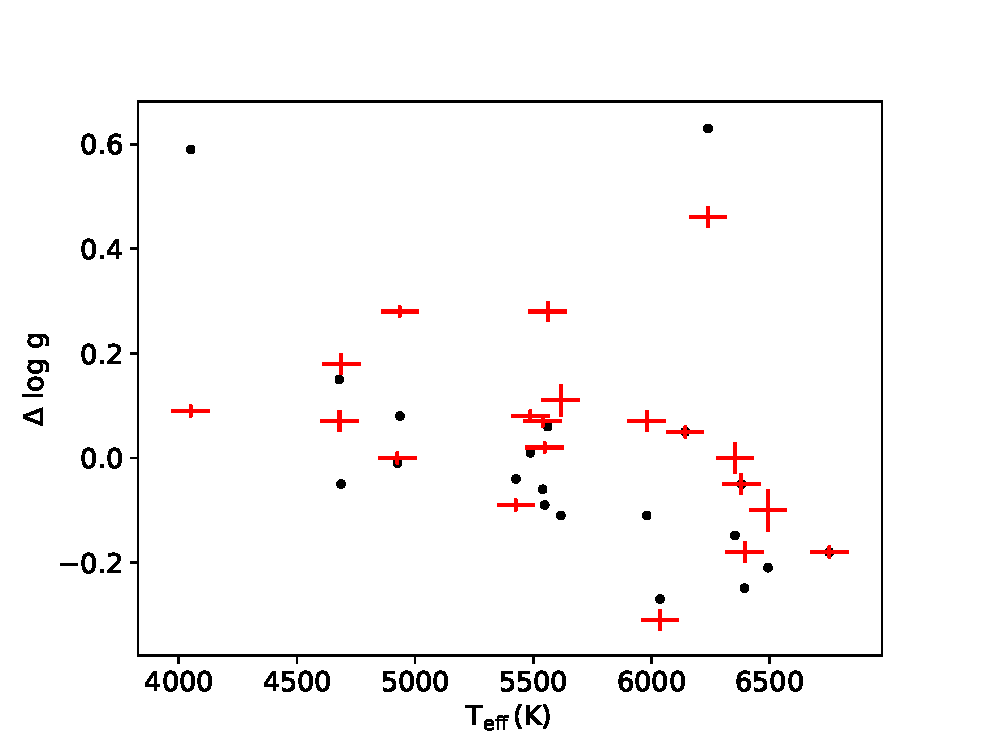
\includegraphics[width=\textwidth]{5-images/mortlogg}
\caption{The difference between spectroscopic $\log g$ and photometric $\log g$ ($\log g_{ph}$ - $\log g_{sp}$) correlated with $\rm T_{\rm eff, \rm wavelet}$ from this work (black) and from D15 (red).}
\label{wavelet:fig:mortlogg}
\end{figure}

  \begin{figure*}[ht!]
\centering
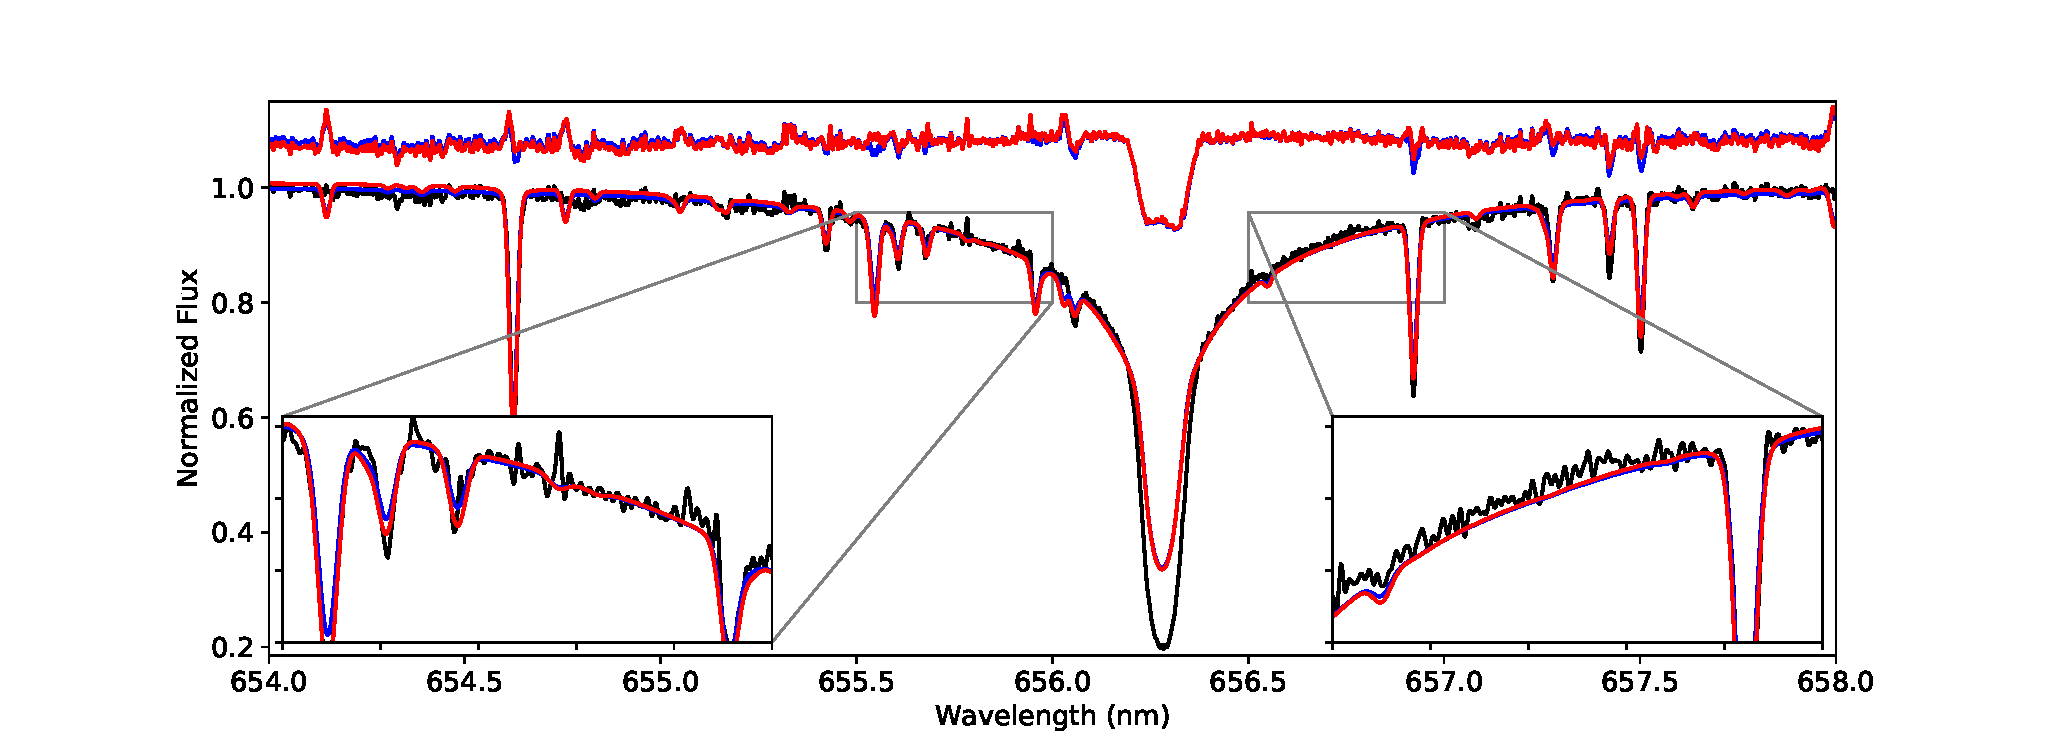
\includegraphics[width=\textwidth, height = 0.4\textwidth]{5-images/WASP20-halpha.eps}
\caption{The H-$\alpha$ region for WASP-20 (black) fitted with the best fitted model from D15 (red) and the best model from this work (blue). The near horizontal lines at flux ~ 1.2 are the residuals between the D15 model (red) or wavelet model (blue) and the spectrum of WASP-20.}
\label{wavelet:fig:WASP-20Halpha}
\end{figure*}


\begin{figure}[ht!]
\centering
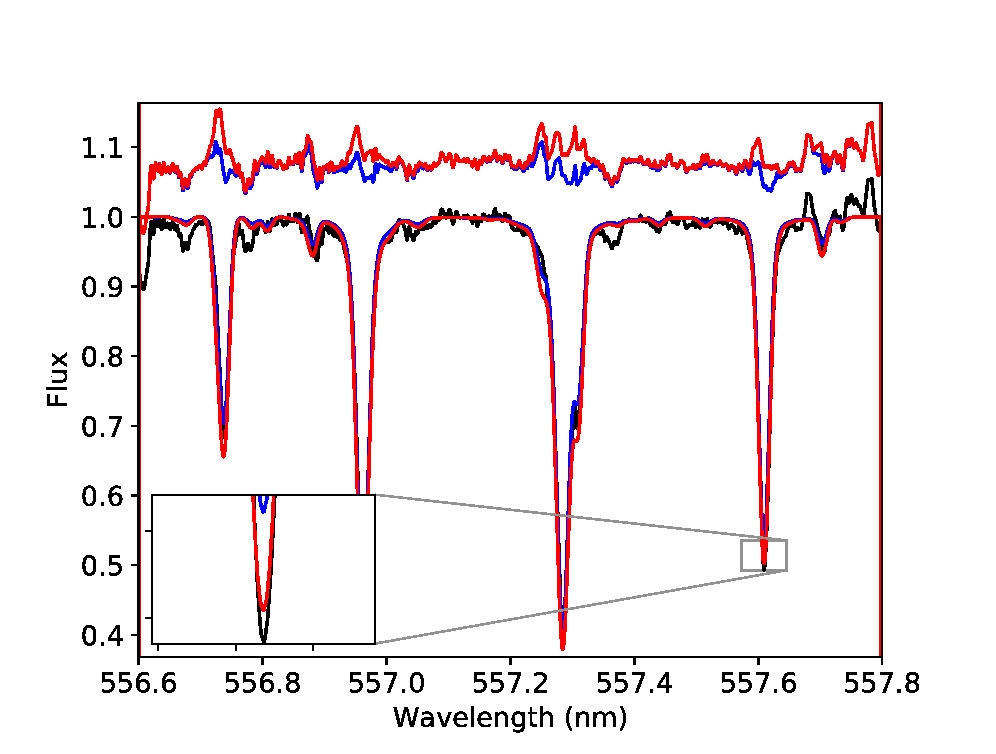
\includegraphics[width=\textwidth]{5-images/Felines}
\caption{Fe lines for WASP-20 alongside the best fitting model from D15 (red) and that from this work (blue). I enlarge one of the cores of an Fe line to highlight that the D15 line-depths are a better match than those found by the wavelet method. }
\label{wavelet:fig:FElines}
\end{figure}


In Fig. \ref{wavelet:fig:WASP-20Halpha} I assessed the  H$\alpha$ region for the model predicted from D15 and this work for the highest-quality spectrum in my sample, WASP-20, with S/N $= 150$. The results from D15 were obtained using a custom line list, whereas I use version 5 of the GES atomic line list provided with iSpec to synthesise the D15 model of WASP-20 using atmospheric parameters, $\nu_{\rm mac}$ and $\nu_{mic}$ from D15. I found both models agree well with the data, with the left wing fitting best and a underestimation in the right wing. The discrepancies between the two wings of the  H$\alpha$ line seen here are the result of the difficulty in calibrating the blaze function in this region of the spectrum.  I found that the majority of Fe line depths are under-predicted with the wavelet method, with the D15 model better matching individual line profiles. This test demonstrates the need to benchmark against well studied stars and visually inspect the best models against the data.


\subsection{Systematic offset in [Fe/H]}\label{wavelet:fe_offset}

\begin{table}
\caption{The performance of the wavelet method using different mother wavelets. Each analysis was performed on WASP-7 using the same method used in Sect. \ref{wavelet:wavelet_benchmark}. }              % title of Table
\label{wavelet:table:wavelet_tab}      % is used to refer this table in the text
\centering                                      % used for centering table
\begin{tabular}{l r r r r c c c c c}          % centered columns (4 columns)
\hline\hline                        % inserts double horizontal lines
Wavelet
& \multicolumn{1}{p{1cm}}{\centering $T_{\rm eff}$  \\ (K)}
& \multicolumn{1}{p{1cm}}{\centering [Fe/H]  \\ ($dex$)}
& \multicolumn{1}{p{1cm}}{\centering $\log g$ \\ ($dex$)}
& \multicolumn{1}{p{1cm}}{\centering $V \sin i$  \\ (km\,s$^{-1}$)} \\
\hline
Daubechies k=4 & 5983 & 0.11 & 4.50 & 17.54\\
Daubechies k=20 & 5975 & 0.11 & 4.36 & 17.55 \\
Harr k=2  & 5962 & 0.11 & 4.34 & 17.52\\
bspline k=20 & 5961 & 0.10 & 4.36 & 17.77\\
\hline                                             %inserts single line
\end{tabular}
\end{table}


\begin{table}
\caption{The regional performance of the wavelet method on WASP-20 using a variety of wavelength ranges. No priors for $\log g$ were used.}              % title of Table
\label{regional_tab}      % is used to refer this table in the text
\centering                                      % used for centering table
\begin{tabular}{l r r r r c c c c c}          % centered columns (4 columns)
\hline\hline                        % inserts double horizontal lines
Range 
& \multicolumn{1}{p{1cm}}{\centering $T_{\rm eff}$  \\ (K)}
& \multicolumn{1}{p{1cm}}{\centering [Fe/H]  \\ ($dex$)}
& \multicolumn{1}{p{1cm}}{\centering $\log g$ \\ ($dex$)}
& \multicolumn{1}{p{1cm}}{\centering $V \sin i$  \\ (km\,s$^{-1}$)} \\

\hline
450\,--\,500\,nm & 5984 & $-$\,0.17 & 4.31 & 3.98  \\
500\,--\,550\,nm & 6076 & $-$\,0.06 & 4.33 & 3.76 \\
550\,--\,600\,nm & 5530 & $-$\,0.34 & 4.00 & 3.60  \\
600\,--\,650\,nm & 6099 & $-$\,0.12 & 4.96 & 3.45\\
400\,--\,600\,nm & 5983 & $-$\,0.11 & 4.50 & 3.63\\
D15 & 6030 & 0.13 & 4.23 & 4.30 \\
 
\hline                                             %inserts single line
\end{tabular}
\tablefoot{50nm windows had 2$^{15}$ samples and the 200nm windows had 2$^{17}$ samples. All were subject to the same analysis in Sect. \ref{wavelet:wavelet_benchmark} with no priors on $\log g$.}
\end{table}


There are many reasons why my method may produce composition offsets when compared with other established techniques. The interested reader should see \cite{26A...601A..38J} for an excellent review on how the specifics of spectroscopic analysis routines affect abundance measurements. One interesting result from \cite{26A...601A..38J} is the effect of continuum normalisation which increased the method-to-method scatter in abundance measurements by up to 0.3\,dex (see their Fig.\,5). Wavelet filtering in my method is an alternate approach to normalisation, and so an offset of around 0.18\,dex is not entirely unexpected. I assessed if there is a systematically lower continuum placement by adding an free parameter, $C_0$, which is a constant to add to the normalised flux of the model spectra before a discrete wavelet transform in the calculation of log-likelihood. I found values of $C_0$ converged to values between $-0.05$ and $0.05$ and did not affect measurements of [Fe/H] by more than $0.05$\,dex; $T_{\rm eff}$ remained the same for all stars within 150\,K and $\log g$ changed by as much as 0.2\, dex. 

I also looked at components unique to the wavelet method. For instance, the mother wavelet used (Daubechies, k=4) may not capture the true line depths when  convolved with a spectrum. I again measured WASP-20 with three alternative wavelets (Daubechies k=20, Harr k=2 and bspline  k=103) across the range 450\,--\,650\,nm  (see Table \ref{wavelet:table:wavelet_tab}). I found the choice of mother wavelet has little influence on the determined composition (and  all other atmospheric parameters) for WASP-20 and I found similar results for the rest of the D15 sample.  It is possible that the resolution of the finest wavelet convolution (2 pixels) is not sufficient to capture iron line depths. To assessed this, I convolved a few iron lines with the Daubechies k=4 kernel and assessed  whether line depths were under-determined. I found this not to be the case, suggesting no degradation of line depths owing to the choice in wavelets. 

Finally, I consider the possibility that there may be instrumental effects at play with the CORALIE \'{e}chelle spectrograph. A discrepancy in EW measurements for WASP-69 (see Fig. 3.19 in D15) suggests this instrument is prone to scattered light \citep{Doyle2015}. This may be partly responsible for the systematic error in the iron abundance when combined with a low-quality spectrum. 

The zero-point of the metalicity scale is a subject of on-going debate (e.g. \citealt{Kraft2004}). However, I can conclude that models using parameters found by D15 (as generated with line lists and atmospheres used in the above work) have better-fitting line depths for the majority of Fe lines in the D15 sample than my predicted models. For this reason, I apply the following correction for the [Fe/H] values of EBLM systems measured with the wavelet method to make them consistent with the metallicity scale of D15:
\begin{equation}\label{composition_correction}
\rm [Fe/H]_{\rm corrected} = \rm [Fe/H]_{\rm measured} + 0.18.
\end{equation}  



\subsection{Systematic trend in $\log g$}

I also observe a negative correlation between residual $\log g$ measurements (wavelet - D15) and $\log g$ measured with the wavelet method (Fig. \ref{doyle:c}). This trend is observed with and without Gaussian priors on $\log g$ from transit photometry. I calculate a Pearson correlation coefficient of -0.501 for measurements with no $\log g$ prior, suggesting a significant negative correlation. I fit this trend with a first-order polynomial and found a gradient of $-0.692$ and a y-intercept of $3.067$. This correlation evaluates to zero at a wavelet $\log g$ value of 4.44. In principle, the following correction can be used to bring my $\log g$ measurements into line with those from D15,

\begin{equation}\label{logg_corr}
\log g_{\rm corrected} = \log g_{\rm wavelet} - 3.067 + 0.692\times \log g_{\rm wavelet}.
\end{equation}
Without knowing the exact cause of this trend, and given the sensitivity of my $\log g$ estimates to the continuum placement,  I am reluctant to advise applying this correction and conclude that the wavelet method cannot reliably estimate $\log g$ beyond confirming a dwarf-like surface gravity. Obtaining $\log g$ from a spectrum is typically done through ionization balance (balancing the iron abundance measured from the Fe
I and Fe II lines). It is also possible to measure  $\log g$  by fitting the wings of gravity sensitive lines (e.g. Mg, Na) using model spectra (the synthesis method). This is essentially how the wavelet method operates (in wavelet space rather than normalised flux space). Accurate determinations of log g from the synthesis method requires detailed element-abundance measurements for gravity-sensitive Na and Mg lines. Estimating the abundances of these elements by scaling from the solar abundance values and applying some correction for $\alpha$ element enhancement will lead to a systematic error in $\log g $ that is difficult to quantify in individual cases. To investigate this further requires another set of comparison stars with independent $\log g$ values (preferably from binary systems where $\log g$ can be accurately measured and not planet transiting systems). 



\subsection{\textbf{Precision of atmospheric parameters}}\label{precision_w}

The high precision of the parameters in Table~\ref{wavelet:table:waspstars} shows that the wavelet method can reliably converge to a well-determined set of atmospheric parameters, but to make use of these parameters I also require a reliable estimate of their true precision that accounts for additional uncertainties due to systematic errors in the data and the models. To obtain a realistic estimate of true precision of the parameters from the wavelet method, $\sigma_{\rm wavelet}$, I compare the results from my method with the correction to [Fe/H] described earlier to those from D15. The standard deviation of the residuals between the measured atmospheric parameters made by D15 and from the wavelet method, $\sigma_{\rm D15 - \rm wavelet}$, is a combination of the uncertainties from methods added in quadrature:
\begin{equation}
\sigma_{\rm D15 - \rm wavelet}^2 = \sigma_{\rm D15}^2 + \sigma_{\rm wavelet}^2,
\end{equation}
where $\sigma_{\rm D15}$ is the quoted error on the atmospheric parameters from D15. There are two extreme cases: the first is that the uncertainty from D15 is negligible (or at least much better than what I can achieve) giving $\sigma_{\rm D15 - \rm wavelet}^2 \approx \sigma_{\rm wavelet}^2$; and the second is that the inter-method discrepancy, $\sigma_{\rm D15 - \rm wavelet}^2$, is negligible leaving uncertainties similar to those quoted by D15. In reality, the absolute uncertainty for the wavelet method is somewhere between these two extremes. I adopt a true precision of each parameter from Table \ref{wavelet:table:doyle_tab} using a uniform prior on $\log g$ which is to assume that $\sigma_{D15} \langle \langle \sigma_{wavelet}$. I suggest applying a correction of $+0.18\,dex$ to [Fe/H] and not to apply a correction to $\log g$. This means precision of $85\, \rm K$ for $T_{\rm eff}$, $0.06\, dex$ for [Fe/H] and $1.35\,kms^{-1}$ for $V \sin i$. The resulting value of $\log g$ is not likely to be reliable but is good enough to confirm dwarf-like gravity around $\log g = $ 4--5 $dex$. I note that these values are comparable to other methods (e.g. \citealt{2010MNRAS.405.1907B}).



\subsection{Spectrum quality}\label{wavelet:spec_quality}

\begin{figure}[ht!]
\centering
\includegraphics[height=15cm,width=12cm]{5-images/snr1.eps}
\caption{Atmospheric parameters from the wavelet method, with no prior on $\log g$, compared to those from D15 ($x_{\rm D15}-x_{\rm wavelet}$) as a function of S/N.}
\label{wavelet:fig:snr}
\end{figure}

\begin{figure}[ht!]
\centering
\includegraphics[width=\textwidth]{5-images/precision.eps}
\caption{Precision of the wavelet method versus S/N for $T_{\rm eff}$ (top left), [Fe/H] (top right), $\log g$ (bottom left), and $V \sin i$ (bottom right) for WASP-20. }
\label{wavelet:fig:precision}
\end{figure}

\begin{figure}[ht!]
\centering
\includegraphics[width=\textwidth]{5-images/accuracy.eps}
\caption{Accuracy of the wavelet method versus S/N for $T_{\rm eff}$ (top left), [Fe/H] (top right), $\log g$ (bottom left), and $V \sin i$ (bottom right) for WASP-20 using the results from D15 as a zero-point.}
\label{wavelet:fig:accuracy}
\end{figure}

In Fig. \ref{wavelet:fig:snr} I plot the difference between atmospheric parameters obtained with the wavelet method (with no priors for $\log g$) to those from D15 as a function of S/N. The sample falls into two categories of quality (those with S/N $\leq$ 90 and those with S/N $\geq$ 120). There is noticeably more scatter in the lower-quality group and suggests that the uncertainty of my atmospheric parameters decreases with a better-quality spectrum. The noise profile of a spectrum depends on observing conditions, properties of the star and the instrument used to make the observations. This is why adding Gaussian noise to a synthetic spectrum until the atmospheric parameters are no longer recoverable does not give a true reflection of a methods robustness to noise. Instead, I use 32 (out of 58) observations of the star with the highest S/N in the D15 sample - WASP-20. I dyadically split up these spectra and median combine them into different sets. The sets of splits used were 1 spectrum (1 set of 32 spectra), 2 spectra (2 sets of 16 spectra), 4  spectra (4 sets of 8 spectra), ..., 32 spectra (32 sets each containing just 1 spectra). I scale S/N from the coaddition of all 58 spectra:
\begin{equation}
\rm S/N = \rm S/N_{58 \, \rm spectra} \times \sqrt{\frac{N_{\rm set}}{58}}.
\end{equation}
Each set was measured with the aforementioned wavelet technique with no prior probability function for $\log g$, and best fitting parameters adopted. The precision and accuracy as a function of S/N are shown in Figs. \ref{wavelet:fig:precision} and \ref{wavelet:fig:accuracy}, respectively. I found that systematic errors dominate for a S/N below 40. A similar result is found by \citet{2014A&A...570A.122S} who measured UVES-FLAMES spectra for FGK stars from the GAIA-ESO survey and found a systematics threshold of S/N$\, \approx 50$.



\section{Conclusion} \label{Conclusion}

I have shown that my method accurately recovers the atmospheric parameters of synthetic spectra from a grid of models using subsets of wavelet coefficients in a Bayesian framework. The same method was applied to the CORALIE spectra of 20 FGK stars which have been analysed independently by measurements of EWs from higher-quality HARPS spectra. From this I determine a precision for the parameters derived from the wavelet method of $85\, \rm K$ for $T_{\rm eff}$, $0.06\, \rm dex$ for [Fe/H] and $1.35\,  \rm kms^{-1}$ for $V \sin i$. Surface gravity, $\log g$, can also be estimated using my method but it is difficult to assessed the precision of this parameter in individual cases. Consequently, I recommend that $\log g$ estimates from my method are only used to decide whether or not a star is a dwarf ($\log g \approx 4.5$). I found an offset in my metallicity scale compared to the results of (\citealt{Doyle2013}, \citealt{Doyle2015}) in the sense that my values of [Fe/H] are lower by 0.18 dex, despite using a consistent solar abundance, and recommend that this offset be applied as a correction to the [Fe/H] values from my method. I found my method is robust for \'{e}chelle spectra with a S/N above 40. Below this value the uncertainty in the measured atmospheric parameters increases to unusable levels. A further development of this method would include a more sophisticated weighting system for the wavelet coefficients beyond the Monte Carlo approach used here. 

My method has already been used to determine the atmospheric parameters of the EBLM~J0555$-$57 \citep{vonBoetticher2017},  which hosts one of the densest main sequence stars currently known. This method is also being used to study other EBLM systems and as part of the on-going exoplanet discovery process of the  WASP survey. For both exoplanet systems and EBLM binaries, the contribution of the companion star to the optical flux is negligible (they are SB1 binaries) and so my method using models of single stars is appropriate, but it would not be suitable for cases where the companion is detectable in the spectrum (SB2 binaries).  I have used wavelet decomposition to measure the atmospheric parameters of all EBLMs presented in this work with the exception of the northern target J1847$+$39. 

%We have optimised our method for the application to spectra from CORALIE, but the same method should be equally applicable to spectra with moderate S/N from other echelle spectrographs. We have implemented the wavelet method in a python module called \textit{waveletspec} which is available upon request. 










% Chapter 7. Methods
%\chapter{Observations}


% Include the table
\begin{table*}
\caption{Summary of observations used to derive stellar atmospheric and orbital solutions for 5 EBLMs observed from the ground. The square brackets indicate the filter corresponding to the preceding number of observations.}              % title of Table
\label{Observeration_table_ground}      % is used to refer this table in the text
\centering                                    % used for centering table
\begin{tabular}{c l l  l l l l l l l l l l l l l }          % centered columns (4 columns)

\hline
\hline
 & J2349$-$32 & J2308$-$46 & J0218$-$31 & J1847$+$39 & J1436$-$13 \\
\hline
J2000.0 \\
$\alpha$  & $23^{\rm h}49^{'}15.23^{"}$ & $23^{\rm h}08^{'}45.66^{"}$ & $02^{\rm h}18^{'}13.24^{"}$ & $18^{\rm h}47^{'}52.34^{"}$ & $14^{\rm h}36^{'}46.42^{"}$\\
$\delta$ & $-32^{\circ}46' 17.5^{"}$ & $-46^{\circ}06^{'}36.6^{"}$  & $-31^{\circ}05^{'}17.3^{"}$ & $+39^{\circ}58^{'}51^{"}$ & $-13^{\circ}32^{'}35.5^{"}$\\
Vmag & 11.53 & 11.36 & 9.96 & 11.73 & 12.48\\
\\
$observations$ \\
WASP  & 8144 & 14,369 & 7872 & 9639 & 53,259 \\
SAAO 1-m  & 345 [I] & 474 [R]  & - & -  & 136 [R]\\
CTIO & - & - & 78 [g'] &- &- \\
& & & 62 [z'] \\
& & & 71 [r'] \\
& & & 70 [z'] \\
HAO  & - & - & - & 605 [CBB] & - \\
& & & & 311 [g'] \\
& & & & 371 [z'] \\
CORALIE & 20 & 19 & 70 & -& 20\\
INT & - & - & - &10 &-\\
\\
$Gaia$ \\
$G$
& $11.448 \pm 0.001$
& $11.381 \pm 0.001$
& $ 9.775 \pm 0.001$
& $11.755 \pm 0.001$
& $12.334 \pm 0.001$\\

$G_{BP} - G_{RP}$
& 0.7209
& 0.7276
& 0.7792
& 0.8177
& 0.7586 \\

parallax [mas]
& $3.851 \pm 0.042$ 
& $2.269 \pm 0.078$
& $3.844 \pm 0.042$
& $3.665 \pm 0.025$ 
& $2.145 \pm 0.051$\\\\

$photometry$ \\
APASS9 [B]  & 
$12.142 \pm 0.039$ &
$12.072 \pm 0.015$ &
$10.519 \pm 0.037$ &
$12.382 \pm 0.021$ &
$12.986 \pm 0.009$ \\

APASS9 [V]  & 
$11.541 \pm 0.010$ &
$11.517 \pm 0.045$ &
$9.903 \pm 0.026$ &
$11.913 \pm 0.022$ &
$12.480 \pm 0.014$ \\

APASS9 [g'] & 
$11.785 \pm 0.013$ &
$11.749 \pm 0.016$ &
$10.202 \pm 0.032$ &
$12.007 \pm 0.031$ &
$12.690 \pm 0.018$ \\

APASS9 [r'] & 
$11.438 \pm 0.033$ &
$11.382 \pm 0.014$ &
$9.779 \pm 0.029$ &
$11.704 \pm 0.006$ &
$12.354 \pm 0.021$ \\

APASS9 [i'] &
$11.317 \pm 0.013$ &
$11.286 \pm 0.006$ &
$9.632 \pm 0.079$ &
$11.548 \pm 0.006$ &
$12.231 \pm 0.064$ \\


TYCHO [B$_{\rm T}$] & 
$12.278 \pm 0.138$ &
$11.801 \pm 0.091$ &
$10.655 \pm 0.039$ &
$12.146 \pm 0.137$ &
- \\

TYCHO [V$_{\rm T}$] & 
$11.593 \pm 0.100$ &
$11.398 \pm 0.108$ &
$9.958 \pm 0.033$ &
$11.766 \pm 0.150$ &
- \\
2MASS [J] & 
$10.530 \pm 0.023$ &
$10.477 \pm 0.022$ &
$8.783 \pm 0.034$ &
$10.682 \pm 0.026$ &
$11.353 \pm 0.027$ \\

2MASS [H] & 
$10.249 \pm 0.022$ &
$10.270 \pm 0.024$ &
$8.555 \pm 0.031$ &
$10.362 \pm 0.032$ &
$11.040 \pm 0.021$ \\

2MASS [K$_{\rm S}$] & 
$10.184 \pm 0.019$ &
$10.166 \pm 0.020$ &
$8.493 \pm 0.025$ &
$10.306 \pm 0.021$ &
$10.987 \pm 0.019$ \\

DENIS [I$_{\rm C}$] & -  & - & - & - & $11.790 \pm 0.030$ \\
DENIS [J] & -  & - & - & - & $11.371 \pm 0.070$ \\
DENIS [K$_{\rm S}$] & -  & - & - & - & $10.912 \pm 0.070$ \\

E(B-V) & 
$0.010 \pm 0.034$ &
$0.007 \pm 0.034$ &
$0.024 \pm 0.030$ &
$0.088 \pm 0.030$ &
$0.072 \pm 0.034$ \\


\end{tabular}
\end{table*}








\begin{table*}
\caption{Summary of observations used to derive stellar atmospheric and orbital solutions for 5 EBLMs observed with K2. The square brackets indicate the filter corresponding to the preceding number of observations. }              % title of Table
\label{Observeration_table_K2}      % is used to refer this table in the text
\centering                                    % used for centering table
\begin{tabular}{c l l  l l l l l l l l l l l l l }  

\hline\hline                        % inserts double horizontal lines
 
 & J0055$+$00 
 & J0457$+$14 
 & J1652$-$19
 & J2217$-$04 \\
 
  
 & \object{EPIC220196587} 
 & \object{EPIC246712205}
 & \object{EPIC205148699}
 & \object{EPIC206500801}\\
 
\hline 
J2000.0 \\

$\alpha$  
& $00^{\rm h}55^{'}13.72^{"}$ 
& $04^{\rm h}57^{'}20.84^{"}$ 
& $16^{\rm h}52^{'}38.52^{"}$ 
& $22^{\rm h}17^{'}58.13^{"}$ \\


$\delta$ 
& $-00^{\circ}07' 54.00^{"}$
& $+14^{\circ}43' 30.40^{"}$
& $-19^{\circ}09' 41.70^{"}$
& $-04^{\circ}51' 52.60^{"}$\\

Vmag 
& 10.96 
& 12.14
& 12.75
& 12.18\\ \\

CORALIE
& 24
& 15
& 14
& 13\\ \\

$K2$ \\
Campaign 
& 8
& 13
& 2
& 3\\

data points 
& 3595
& 3703
& 2601
& 3199\\

Usable transits 
& 7
& 23
& 9
& 9\\ \\

$Gaia$ \\
$G$-mag
& $10.912 \pm 0.001$
& $11.916 \pm 0.001$
& $12.413 \pm 0.001$
& $12.003 \pm 0.001$ \\

$G_{BP} - G_{RP}$
& 0.8342
& 0.8439
& 1.0134
& 1.0294 \\

Parallax [mas]
& $3.158 \pm 0.062$ 
& $1.419 \pm 0.039$
& $2.081 \pm 0.113$
& $2.480 \pm 0.099$ \\ \\

$photometry$ \\
APASS9 [B]   
& $11.711 \pm 0.027$
& $12.677 \pm 0.036$
& $13.344 \pm 0.026$
& $13.047 \pm 0.053$ \\

APASS9 [V]  
& $11.043 \pm 0.032$
& $12.088 \pm 0.034$
& $12.614 \pm 0.043$
& $12.221 \pm 0.030$ \\

APASS9 [g']  
& $11.339 \pm 0.021$
& $12.374 \pm 0.035$
& $12.949 \pm 0.031$
& $12.582 \pm 0.040$ \\

APASS9 [r'] 
& $10.884 \pm 0.033$
& $11.920 \pm 0.021$
& $12.391 \pm 0.047$
& $11.957 \pm 0.024$ \\

APASS9 [i'] 
& $10.745 \pm 0.059$
& $11.772 \pm 0.072$
& $12.113 \pm 0.065$
& $11.922 \pm 0.215$ \\

2MASS [J] 
& $9.899 \pm 0.023$
& $10.801 \pm 0.023$
& $11.027 \pm 0.023$
& $10.749 \pm 0.022$ \\

2MASS [H] 
& $9.613 \pm 0.027$
& $10.663 \pm 0.032$
& $10.649 \pm 0.025$
& $10.404 \pm 0.022$ \\

2MASS [K$_{\rm S}$] 
& $9.534 \pm 0.021$
& $10.529 \pm 0.021$
& $10.554 \pm 0.022$
& $10.296 \pm 0.023$ \\

E(B-V)
& $0.023 \pm 0.034$
& $0.350 \pm 0.034$
& $0.298 \pm 0.034$
& $0.09 \pm 0.034$ \\

\hline


\end{tabular}
\end{table*}


Measuring the masses and radii of EBLM systems requires two types of data. The first type are spectroscopic observations which are taken at different phases of an EBLMs orbit. Spectra have two uses in this work: 1) they provide radial velocity measurements and 2) they can be co-added to estimate atmospheric parameters. I also use photometric colours to fit the spectral energy distribution to measure the photometric temperature and reddening. The second data type is transit photometry which sets the scale of each component. The quality of WASP photometry is not good enough to measure masses and radii to the desired precision of a few percent. To this end, I obtained higher-quality follow-up photometry which was used to determine the orbital solution. In the following sections I detail the origin and processing of data used in this work; this is summarised in Table \ref{Observeration_table_ground} \& \ref{Observeration_table_K2}. 



\section{Photometric colours}

Photometry for each target was extracted from the following catalogues: B$_{\rm T}$ and V$_{\rm T}$ magnitudes from the Tycho-2 catalogue \citep{2000A26A...355L..27H}; B, V, g$^{\prime}$, r$^{\prime}$ and i$^{\prime}$ magnitudes from data release 9 of the AAVSO Photometric All Sky Survey (APASS9; \citealt{2016yCat.2336....0H}; J, H and K$_{\rm s}$ magnitudes from the Two-Micron All-Sky Survey (2MASS; \citealt{2006AJ....131.1163S}; i$^{\prime}$, J and K magnitudes from the DEep Near-Infrared Southern Sky Survey (DENIS; \citealt{1997Msngr..87...27E}). The reddening maps by \citet{2011ApJ...737..103S} were used to estimate the total line-of-sight extinction in the direction of each target, ${\rm E}({\rm B}-{\rm V})$. Values of ${\rm E}({\rm B}-{\rm V})$ were calculated using the NASA/IPAC Extragalactic Database (NED) operated by the Jet Propulsion Laboratory, California Institute of Technology\footnote{https://ned.ipac.caltech.edu/help/extinction\_law\_calc.html}. Not all EBLMs have photometry in all catalogues; those that do are reported in Tables \ref{Observeration_table_ground} \& \ref{Observeration_table_K2}.

\section{Gaia}

\begin{figure}
    \centering
    \includegraphics[scale=0.5]{6-images/GaiaDR2Passbands.png}
    \caption{The coloured lines in the figure show the revised passbands for $G$, $G_{\rm BP}$ and $G_{\rm RP}$ (green: $G$; blue: $G_{\rm BP}$; red: $G_{\rm RP}$), defining the Gaia DR2 photometric system. The thin, grey lines show the nominal, pre-launch passbands published in Jordi et al. 2010, used for Gaia DR1. Image taken from \textit{www.cosmos.esa.int}.}
    \label{methods:fig:gaia_EBLMs_passband}
\end{figure}


\begin{figure}
    \centering
    \includegraphics{6-images/Gaia_EBLMs.png}
    \caption{The $M_{\rm G}$-$G_{\rm BP}-G_{\rm RP}$ plane for 100 randomly selected source fields (black). The EBLMs used in the work are marked in red. }
    \label{methods:fig:gaia_EBLMsmy_label}
\end{figure}

% look here
% https://www.cosmos.esa.int/documents/29201/1770596/Lindegren_GaiaDR2_Astrometry_extended.pdf/1ebddb25-f010-6437-cb14-0e360e2d9f09
% Expand this section
% re- plot G Mag e.t.c

The second Gaia data release (Gaia DR2; \citealt{2018A&A...616A..10G}) provides mean flux counts in three bands -- $G$, $G_{\rm BP}$ and $G_{\rm RP}$ (see Fig. \ref{methods:fig:gaia_EBLMs_passband}). The $G$-band has a wider wavelength coverage and is optimised to determine astrometric solutions. The mean magnitudes $G_{\rm BP}$ and $G_{\rm RP}$ provide a ``slice'' through the spectral energy distribution of stars and reveal how red or blue a star is. I obtained the mean $G$, $G_{\rm BP}$ and $G_{\rm RP}$ magnitudes along with parralax measurements for all nine EBLM systems from Gaia DR2 using the Gaia archive\footnote{https://gea.esac.esa.int/archive} (Tables \ref{Observeration_table_ground} \& \ref{Observeration_table_K2}). There is evidence of systematic offsets in parallax measurements from Gaia DR2 (e.g. \citealt{2018ApJ...862...61S}) which is likely correlated with on-sky positions ($\alpha$ \& $\delta$), $G$ and $G_{\rm BP}$ - $G_{\rm RP}$ \citep{2018A&A...616A...2L}. Because the masses, radii and age of M-dwarfs in EBLMs in work do not depend on these results, I did not apply corrections to the parallax. The parallaxes and mean magnitudes are only used to briefly discuss tertiary components and volume-limited samples. I plot the position of all EBLMs in the $M_{\rm G}$-$G_{\rm BP}-G_{\rm RP}$ plane using data from 100 randomly selected source fields (Fig. \ref{methods:fig:gaia_EBLMsmy_label}). 

\section{Photometry: WASP}\label{WASP}

The WASP survey \citep{PollaccoSkillenCollierCameronEtAl2006} operates two survey instruments: one at the South African Astronomical Observatory (SAAO), South Africa, and another at the Observatorio del Roque de los Muchachos, La Palma.  Each instrument consists of an equatorial fork mount with eight cameras with 200-mm lenses and 2k$\times$2k CCD detectors. Each camera coveres approximately 64 square degrees per exposure. The data are processed by a detrending algorithm which was developed from the \textsc{SysRem} algorithm of \citet{2005MNRAS.356.1466T} and that is described by \citet{2007MNRAS.375..951C}. In July 2012, lenses on the southern installation (WASP-South) were changed to 85-mm with f/1.2 to search for brighter exoplanet hosts \citep{Smith2014}. Data from 85-mm lenses were not used in this study.

Photometry from the WASP cameras can suffer from a large amount of scatter due to clouds, instrumental artefacts, scattered light and other non-optimal observing conditions. I cleaned the data by removing points that were not detrended in the standard WASP reduction pipeline and removed points more than 0.5\,mag from the median magnitude of each star. Additional cleaning of the light curve was done by comparing each night of data to a phase-folded light curve binned into 500 phase bins. Any measurement $3$-$ \sigma$ or more from the mean in each bin was excluded. The entire night of data was excluded if more than a quarter of the night's data was excluded this way or if there are fewer than 10 observations. The binned light curve is then inspected by eye to further exclude bad data points.

\section{Photometry: SAAO 1-m}

The SAAO hosts an equatorial-mounted 1-m telescope built by Grubb and Parsons that is equipped with an STE4 CCD camera with 1024\,$\times$\,1024 pixels. This camera was operated in $2 \times 2$ binning mode to reduce readout time. I observed a single transit for J2349$-$32 on 18 October 2016 and J2308$-$46 on  12 October 2016 using $I$ (exposure time of $t_{\rm exp}$ = 50\,s) and $R$ ($t_{\rm exp}$ = 40\,s) Bessel filters. Jess Kirkby-kent observed J1436$-$13 on 23 April 2017 in the $R$ ($t_{\rm exp}$ = 40\,s) Bessel filter. Photometry was extracted using standard aperture photometry routines \citep{Southworth2009} and uncertainties were estimated from photon counting statistics. A by-eye approach was used to clean the light curve and select the best comparison star in the $5' \times 5'$ field. A slow variation in differential magnitude with time was observed corresponding to changes in the effective airmass. To correct for this, I defined out-of-transit regions and then used the IDL/AMOEBA\footnote{http://www.harrisgeospatial.com/docs/AMOEBA.html} routine to fit a polynomial which minimised the square of the magnitude residuals. I then divided this trend resulting in light curves which were normalised to zero differential magnitude.  


\section{Photometry: HAO}

\begin{figure}[htb]

  \centering
  \includegraphics{6-images/CBB_response.eps}
  \caption{The response function of the HAO+CBB instrument. The atmospheric transmission is plotted in black, the transmission of the HAO telescope in blue-solid, the CBB filter in green and CCD response in yellow. The final response of HAO-1 with the CBB filter is plotted in red-dashed along with the K2 transmission (blue-dashed). The atmospheric transmission line originated from equations for Rayleigh, aerosol and ozone extinction vs. wavelength for Palomar Observatory \protect\citep{1975ApJ...197..593H}. Coefficients were adjusted until they agreed with observations of extinction at HAO over a few dates.}
  \label{HAO_CBB}
\end{figure}


\begin{figure}[htb]
  \centering
  \includegraphics[scale=0.8]{6-images/kepVShao.eps}
  \caption{The difference in theoretical intensity acoss the stellar disk for the HAO+CBB filter and the Kepler/K2 Filter as a function of the angle between a line normal to the stellar surface and the line of sight of the observer ($\gamma$) for J1847$+$39. }
  \label{kepVShao}
\end{figure}

Optical photometry for J1847$+$39 was provided by Bruce Gary at the Hereford Arizona Observatory (HAO). Three separate transits were observed with a Meade 14-inch LX200GPS telescope. The first was obtained with the clear blue-blocking filter (CBB) on 9 October 2009 with $t_{\rm exp} = 100$\,s. The second was with a $g'$ filter on 18 May 2011 with $t_{\rm exp} = 60$\, s. The last was with a $z'$ filter on 15 June 2010 with $t_{\rm exp} = 60$\, s. Aperture photometry was extracted using standard photometry routines with systematic trends removed and outliers rejected.  I used transmission information of the telescope throughput, atmosphere, filter and CCD\footnote{http://www.brucegary.net/HAO/} to calculate the final transmission of HAO with the CBB filter (see Fig.~\ref{HAO_CBB}). I used the four-parameter limb-darkening look-up table for the K2 passband instead of the CBB filter due to the similarity in final transmission since I do not have access to a four-parameter look-up table for the CBB filter. In Sect.~\ref{limb_darkening_section} I fit light curves
using the two-parameter quadratic limb-darkening instead of the Claret law. The final response function in Fig.~\ref{HAO_CBB} is used  along with estimates of stellar atmospheric parameters (from Sect. \ref{methods:SED} \& \ref{methods:atmospheric_parameters}) to calculate quadratic coefficients using \textsc{ldtk} \citep{Parviainen2015}. 

The discrepancy between the K2 and HAO+CBB pass-band differ in the blue where the limb-darkening is most significant. I assessed this by using \textsc{ldtk} to synthesise intensity profiles for J1847$+$39 across the stellar disk for each pass-band and calculate the discrepancy as a function of $\gamma$ (the angle between a line normal to the stellar surface and the line of sight of the observer; Fig. \ref{kepVShao}). The K2 pass-band emits 2.5\,\% less flux than what would be observed with HA0+CBB towards the limb. I calculated quadratic limb-darkening coefficients for the K2 pass-band to be $u_1 = 0.496 \pm 0.050$, $u_2 = 0.157 \pm 0.050$ and for the HAO+CBB pass-band to be $u_1 = 0.468 \pm 0.050$, $u_2 = 0.148 \pm 0.051$. These are comparable within 1-$\sigma$ and so adopting the K2 pass-band for J1847$+$39 will have a negligible effect on the transit shape.


\subsection{Photometry: CTIO}

J0218-31 was observed on 14 November 2010 with the CTIO-0.9-m telescope and Tek2K CCD camera. The detector consists of a 2K$\times$2K array of $15\mu m$ pixels placed at Cassegrain focus giving a $0.4^{\prime\prime}$/pixel plate scale. Thus the entire array projects to a $13.7^{\prime}$ FOV.   The observed signal is fed into four amplifiers causing the raw images to have a quadrant effect with the readnoise between 3.9-4.5~$e^{-}$ and gain of 2.5-2.8~$e^{-}$/ADU, depending on the amplifier. The detector has a readout time of 39 seconds and a 60,000 count well depth before non-linearity sets in $1\times 1$ binning mode.

J0218-31 and the surrounding field were monitored throughout the night using the Sloan $griz$ filter set alternating continuously between all four filters. Exposure times were chosen to maximise the flux in the target star and nearby reference stars while keeping the peak pixel value in J0218$-$31 below $60,000$ counts. The telescope was defocused to allow for longer exposure times to build up signal in the fainter reference stars without saturating J0218-31. They adopted an exposure time of 10~seconds for the $g^{\prime}$, $r^{\prime}$, and $i^{\prime}$--band observations and longer exposures of 15~seconds in the $z^{\prime}$ filter where the detector is less sensitive. An overall light curve cadence of approximately 3.3 minutes was achieved in each filter accounting for the exposure times,  the read out time, and filter changes. The light curves were created from approximately 75 images taken in each filter during the single observing night.

A set of 11 bias calibration frames and 11 dome flat fields in all four filters were  obtained at the beginning of the observing night. The images were processed in a standard way using routines written by L.\ Hebb in the IDL programming language.  Each of the four amplifiers was processed independently.  All object and calibration frames were first overscan corrected (by subtracting a line-by-line median overscan value), bias subtracted and then trimmed.  Stacked bias images were created by averaging all bias frames observed each night and subtracted from all science  and flat-field frames.  All dome flats were averaged into a single dome flat in each filter and then applied to the trimmed and bias-corrected science images. 

Source detection and aperture photometry were performed on all processed science images using the Cambridge Astronomical Survey Unit catalogue extraction software \citep{2001NewAR..45..105I}. The  software  has  been  compared  with  SExtractor \citep{1996A26AS..117..393B} and found to be very similar in the completeness, astrometry and photometry tests.\footnote{\url{https://www.ast.cam.ac.uk/ioa/research/vdfs/docs/reports/simul/index.html}} This photometry software was applied to all processed images of J0218-31.  Adopting conservative parameters to define the detection threshold, the target star and dozens of fainter stars in the field were detected in each image.  Aperture photometry was performed on all detected stars using a 5~pixel radius circular aperture, which was selected to match the typical seeing. Five bright, non-variable reference stars were selected from the many detected stars and used to perform differential photometry on the target star.  In each image, the flux from all reference stars was summed into a single \textit{super} comparison star that was divided by the aperture flux from J0218-31 and converted to a differential magnitude.

\section{Photometry: K2}

The Kepler mission was launched in 2009 and spent over four years monitoring over 150,000 stars in the constellations of Cygnus and Lyra\footnote{https://keplerscience.arc.nasa.gov/objectives.html}. The spacecraft has a 0.95-m Schmidt telescope
with a 110-square degree field of view imager (pixel scale of 4"/ pixel). The primary science goal of Kepler was to detect and characterise terrestrial planets ($R_p < 2.5\,R_{\oplus}$) which reside in the habitable zone of Sun-like stars. Observations for tens of thousands of stars with short cadence (1-min) and many more thousands with long cadence (30-min) lead to the discovery of many exoplanet (e.g. \citealt{2013ApJ...768...14W}; \citealt{2012ApJ...747..144M}; \citealt{2013ApJ...777....3N}) and eclipsing binary systems (e.g. \citealt{2011Sci...331..562C}; \citealt{2011ApJS..197....4W}; \citealt{2011ApJ...736L...4S}). 

Kepler exceeded its nominal mission lifetime (3 years) by 1 year until the loss of the second of four reaction wheels in May 2013. In the following months the mission was rebranded "K2" - a name chosen to honour the two remaining reaction wheels or the second Kepler mission \citep{2014PASP..126..398H}. The K2 mission consists of sequential observing \textit{campaigns} in the ecliptic plane. This is so the torque excerpted on the spacecraft by solar wind pressure can be balanced with altitude thrusters and the two remaining reaction wheels to control pointing. The pointing is significantly worse than the original Kepler mission but the photometric quality approaches that of the original mission after decorrelation of the position-dependent instrument noise. Four EBLMs with spectroscopic orbits published by \citet{Triaud2017} have been observed with K2 (J0055$+$00, J0457$+$14,  J1652$-$19 and J2217$-$04). In the following sections I describe how  photometry was extracted from target pixel files and how I corrected for position-dependent instrumental noise.


\subsection{Extraction}\label{observations:K2:extract}

The target pixel files for each target were acquired from the Mikulski Archive for Space Telescopes (MAST\footnote{archive.stsci.edu}). I used data from Gaia DR2 to inform how masks were created for the target pixel files. For J0055$-$00, J0457$+$14 and J2217$-$04 I found no significant ($\Delta G < 6$) companions within 1' so I choose masks which match the shape of the stellar profile of the 100$^{th}$ target pixel file (Fig. \ref{observations:target_pixel_files}). For J1652$-$19 I found three close companions within 20" eastwards (Fig. \ref{observations:J1652}). The brightest ($\Delta G = 3.33$) is 14" away at a position angle (PA) of 107$^{\circ}$. This, and the other two fainter companions at PA = 85$^{\circ}$ ($\Delta G = 4.28$) and PA = 54$^{\circ}$ ($\Delta G = 4.17$) may be visible in the target pixel files. If I used full-frame photometry I could expect up to 9\% contamination. I excluded these stars by creating a box-like mask at the east and south side of J1652$-$19. The pointing precision (estimated from centroiding; Sect. \ref{observations:K2:detrending}) is above 1 pixel and so very little flux from the three nearby stars entered into the aperture. I used the \textsc{kepextract} function \citep{pyke3} to extract raw photometry using the masks created for each system. 

 \begin{figure*}
\centering
 \begin{subfigure}[b]{0.5\linewidth}
    \centering
    \includegraphics[width=\linewidth]{6-images/EPIC220196587_PIXEL_FILE.png} 
    %\caption{} 
    \label{EPIC220196587_PIXEL_FILE} 
    \vspace{4ex}
  \end{subfigure}%% 
  \begin{subfigure}[b]{0.5\linewidth}
    \centering
    \includegraphics[width=\linewidth]{6-images/EPIC246712205_PIXEL_FILE.png} 
    %\caption{} 
    \label{EPIC246712205_PIXEL_FILE} 
    \vspace{4ex}
  \end{subfigure} 
  \begin{subfigure}[b]{0.5\linewidth}
    \centering
    \includegraphics[width=\linewidth]{6-images/EPIC205148699_PIXEL_FILE.png} 
    %\caption{} 
    \label{EPIC205148699_PIXEL_FILE} 
  \end{subfigure}%%
  \begin{subfigure}[b]{0.5\linewidth}
    \centering
   \includegraphics[width=\linewidth]{6-images/EPIC206500801_PIXEL_FILE.png}
    %\caption{} 
    \label{EPIC206500801_PIXEL_FILE} 
  \end{subfigure} 
  \caption{The 100$^{th}$ target pixel frame for all EBLM systems. Red dots indicate a pixel that was used to in the aperture photometry using \textsc{pyke}. }
  \label{observations:target_pixel_files}   
\end{figure*}


\begin{figure}
    \centering
    \includegraphics{6-images/J1652.png}
    \caption{The 2MASS finder image of J1652$-$19. Red apertures mark significant stars in the field with Gaia magnitudes labelled. The green box approximates the extent of the K2 pixel files for J1652$-$19 (Fig. \ref{observations:target_pixel_files}).}
    \label{observations:J1652}
\end{figure}




\subsection{De-trending}\label{observations:K2:detrending}

The \textsc{kepextract} function fitted a 2-dimensional Gaussian to the target pixel files in each frame to measure each stars CCD position as a function of time. I used the \textsc{k2sc} algorithm \citep{2016MNRAS.459.2408A} to detrend against time, x-position and y-position using Gaussian processes. I used an exponential-squared kernel provided by the \textsc{george} with the \textsc{detrender} function \citep{hodlr} provided with \textsc{k2sc}. This was used to predict variations in the out-of-transit photometry correlated with time and pixel positions. The remaining outliers between transits were detected using basic iterative sigma-clipping, where a data point was excluded if the flux value was over 5-$\sigma$ from median out-of-eclipse flux level. Although I observed significant "jumps" in photometry continuum levels and evolving noise profiles, I assumed that the remaining variation is caused by stellar activity/binary interaction.

		


\section{Spectroscopy: CORALIE}

CORALIE is a fiber-fed \'{e}chelle spectrograph installed on the 1.2-m Leonard Euler telescope at the ESO La Silla Observatory and has a resolving power R = 50,000\,--\,60,000 \citep{2001A&A...379..279Q,Wilson2008}. The spectra used in this study were all obtained with an exposure time $t_{\rm exp} = 600$\,s. Observations of J0218$-$31 include spectra obtained through the transit that show the Rossiter-McLaughlin effect. The spectra for each star were processed with the CORALIE standard reduction pipeline \citep{26AS..119..373B}. Radial velocity measurements were obtained using standard cross-correlation techniques (using numerical masks) and checked for obvious outliers \citep{Triaud2017}. Each spectrum was corrected into the laboratory reference frame and co-added onto a common wavelength range. Maximum and median filters were applied to identify continuum regions which were fitted with spline functions (one every nm) to normalise the spectra (a standard function within \textsc{ispec} v20161118; \citealt{Blanco-Cuaresma2017}). 


\section{Spectroscopy: INT}

Spectra for J1847$+$39 were obtained using the intermediate dispersion spectrograph (IDS) mounted on the 2.5-m Isaac Newton telescope (INT) at the Roque de Los Muchachos Observatory. The 235-mm camera and EEV10 CCD detector was used with the H1800V grating to obtain spectra in a small region around the H$\alpha$ line with R$\approx$10,000\footnote{Calculated from http://www.ing.iac.es/}. A total of 10 spectra were obtained for J1847$+$39 with an exposure time $t_{\rm exp} = 600$-$900$\, s. Radial velocity measurements were extracted using cross-correlation routines provided within \textsc{ispec}. I used a synthetic F0 spectrum as a template with a mask applied to the core of the H$\alpha$ line. A Gaussian function was fitted to the peak in each cross-correlation function to obtain the radial velocity measurement (the peak of the Gaussian function), and uncertainty (standard deviation of the Gaussian function). Each spectrum was corrected into a laboratory reference frame and co-added onto a common wavelength range. The relatively small wavelength range does not permit the use of maximum and median filters to normalise the spectra. I instead identified suitable continuum regions by-eye and normalised the spectrum using a second-order polynomial fit by least-squares.  

\section{Lucky imaging}

The lucky-imaging technique (e.g. \citealt{2006A&A...446..739L}) was used to obtain high-resolution images of J2308$-$46, J2349$-$32, J0055-00, J1652-19 and J2217-04 in July 2017, in order to search for stars contributing contaminating light, as well as potential bound companions to the eclipsing binaries. The observations were conducted using the Two Colour Instrument (TCI) on the Danish 1.54-m Telescope at La Silla Observatory. The TCI consists of two Electron Multiplying CCDs capable of imaging simultaneously in two passbands at a frame rate of $10$\,Hz, with a $40"\times40$" field of view. The `red' arm has a passband similar to a combined $i+z$ filter or the Cousins $I$ filter, whilst the `visible' arm has a mean wavelength close to that of the Johnson $V$ filter. A detailed description of the instrument  can be found in \citet{2015A26A...574A..54S} and  the lucky imaging reduction pipeline is described by \citet{2012A&A...542A..23H}.

The observations and data reduction were carried out using the method outlined in \citet{2018A26A...610A..20E}, and is briefly described here. Both targets were observed for 170\,s. The raw data were reduced automatically by the instrument pipeline, which performs bias and flat frame corrections, removes cosmic rays, and determines the quality of each frame, with the end product being ten sets of stacked frames, ordered by quality. The data were run through a custom star-detection algorithm that is described in \citet{2018A26A...610A..20E}, which is designed to detect close companion stars that may not be fully resolved.

% Chapter 7. Methods
%\chapter{Methods}

\section{SED fitting}\label{methods:SED}

Empirical colour--effective temperature relations were used used to estimate the effective temperature of the primary star in each system. Such measurements were used to complement our spectroscopic analysis and to provide a measurement of reddening. They were not used to interpolate stellar models and inform limb-darkening coefficients. I also assume that the flux contribution from the M-dwarf companion is negligible compared to the F-type star.

 My model for the observed photometry has the following parameters -- g$^{\prime}_{0}$: the apparent g$^{\prime}$-band magnitude corrected for extinction; $T_{\rm eff}$, the effective temperature; E$({\rm B}-{\rm V})$, the reddening to the system; and $\sigma_{\rm ext}$, the additional systematic error added in quadrature to each measurement to account for systematic errors. For each trial combination of these parameters the empirical colour -- effective temperature relations of \cite{2013ApJ...771...40B} were used to predict the apparent magnitudes of the  star in each of the observed bands. The transformation between the Johnson and 2MASS photometric systems is the same as \citet{2013ApJ...771...40B}. The  Cousins I$_{\rm C}$ band was used as an approximation to the DENIS Gunn i$^{\prime}$ band and the 2MASS K$_{\rm s}$  as an approximation to the DENIS K band (see Fig. 4 of \citealt{2005ARA26A..43..293B}). Table 3 of \citet{2000PASP..112..961B} was interpolated to transform the Johnson B, V magnitudes to Tycho-2 B$_{\rm T}$ and V$_{\rm T}$ magnitudes. This assumed that the extinction in the V band is $3.1\times {\rm E}({\rm B}-{\rm V})$. Extinction in the SDSS and 2MASS bands is calculated using A$_{\rm r} = 2.770\times {\rm E}({\rm B}-{\rm V})$ from \citet{2003A26A...401..781F} and extinction coefficients relative to the r$^{\prime}$ band taken from \citet{2014MNRAS.440.3430D}.

The reddening maps by \citet{2011ApJ...737..103S} were used to estimate the total line-of-sight extinction in the direction of each target, ${\rm E}({\rm B}-{\rm V})_{\rm map}$. This value is used to impose the following (unnormalized) prior on $\Delta = {\rm E}({\rm B}-{\rm V}) - {\rm E}({\rm B}-{\rm V})_{\rm map}$:

\begin{equation}\label{SED_EBV_reddening}
P(\Delta) =  \left\{ \begin{array}{ll} 1 & \Delta \le 0 \\ \exp(-0.5(\Delta/0.034)^2) & \Delta > 0 \\ \end{array} 
\end{equation}
%
The constant 0.034 is taken from \citet{2014MNRAS.437.1681M} and is based on a comparison of ${\rm E}({\rm B}-{\rm V})_{\rm map}$ to ${\rm E}({\rm B}-{\rm V})$ determined using Str\"{o}mgren photometry for 150 A-type stars. The EBLM sample observed with K2 had significantly more reddening than the ground-based sample and the priors described in Eqn. \ref{SED_EBV_reddening} force the sampler to unrealistically low values of ${\rm E}({\rm B}-{\rm V})$. For these four EBLMs, I used a modified prior which only included a Gaussian component:
%
\begin{equation}\label{SED_EBV_reddening_moddified}
P(\Delta) =   \exp(-0.5(\Delta/0.034)^2). 
\end{equation}
%
I used {\sc emcee} \citep{2013PASP..125..306F} to sample the posterior probability distribution (PPD) my our model parameters. {\sc{emcee}} uses affine-invariant ensemble sampling (parallel stretch move algorithm; \citealt{Goodman2010}) to split Markov chains into sub-groups and update the position of a chain using the positions of chains in the other subgroups. The algorithms affine-invariance can cope with skewed probability distributions and generally has shorter autocorrelation times than a classic Metropolis-Hastings algorithm. The empirical colour--temperature relations I have used are valid over the approximate range T$_{\rm eff} = 3450$\,K to 8600\,K.  %Systems where the star has an effective temperature near one of these limits may introduce bias because I exclude trial solutions with any T$_{\rm eff}$ value outside this range. 
Between these limits uniform priors were used on the values of T$_{\rm eff}$. I used uniform priors for g$^{\prime}_{0}$. I sampled 10,000 steps from 100 walkers as a burn-in. A further 10,000 steps were drawn and the step with the highest likelihood value is selected,  with uncertainties equal to the standard deviation of each parameter in the second chain. An example posterior probability distribution for J2349$-$32 is shown in Fig. \ref{methods:fig:SED_J2349-32}; the  PPDs for the other targets are along with residuals (observed magnitudes - calculated magnitudes) are shown in Appendix \ref{appendix:SED_fits}.


\begin{figure}
    \centering
    \includegraphics[scale=0.6]{7-images/SED_corner_J2349-32.eps}
    \caption{The posterior probability distribution of EBLM J2349$-$32 from photometric fitting. Over-plotted are the 68\%, 95\% and 99.7\% contours.}
    \label{methods:fig:SED_J2349-32}
\end{figure}







\section{Spectroscopic analysis}\label{methods:atmospheric_parameters}

\subsection{CORALIE - wavelet analysis}\label{methods:spectroscopy:wavelet}

The CORALIE spectra observations and reduction were carried out using the method outlined in Chapter \ref{chapter:wavelet} and \citet{2018A&A...612A.111G}, which is briefly describe here. I co-added the spectra and re-sample between 450-650\,nm with $2^{17}$ values. I calculated the wavelet coefficients $W_{i=4-14, k}$ (see Fig. \ref{fig:wavelet:filt} for visual justification of our choice of wavelet coefficients) and fit the same coefficients with model spectra in a Bayesian framework. I initiated 12 walkers and generate 10,000 draws as a burn-in phase. I sampled a further 10,000 draws to sample the PPDs for $T_{\rm eff}$, [Fe/H], $V\sin\,i$ and $\log g$. \citet{2018A&A...612A.111G} note that an [Fe/H] offset of -0.18\,dex which I correct for using Eqn. \ref{composition_correction}. I also note a  significant trend in $\log g$ with $T_{\rm eff}$ which I do not correct. The wavelet method for CORALIE spectra can determine $T_{\rm eff}$ to a precision of $85$\,K, [Fe/H] to a precision of 0.06\,dex and $V \sin i$ to a precision of 1.35\,km\,s$^{-1}$ for stars with $V \sin i$ $\geq$ 5\,km\,s$^{-1}$. However, measurements of $\log g$ are not reliable beyond confirming dwarf-like gravity ($\log g \approx 4.5$). Subsequently, I fitted the wings of the magnesium triplets with spectral synthesis by fixing $T_{\rm eff}$, [Fe/H] and $V\sin i$ and changing $\log g$ until an acceptable fit was found. 

\subsection{INT - synthesis}

INT observations of J1847$+$39 are unsuitable for wavelet analysis as only a small wavelength region around the H$\alpha$ line was observable with the H1800V grating.  The spectral synthesis technique was used to measure $T_{\rm eff}$ from the wings of the H$\alpha$ line and mean [Fe/H] from 11 unblended Fe lines around the H$\alpha$ line; I assumed an instrumental resolution of R$\approx$10,000. I determined a "good fit" by synthesising models which best match the spectra in shape and depth. This is assessed \textit{by-eye}.  I used the same model spectra used in Chapter \ref{chapter:wavelet} and Sect. \ref{methods:spectroscopy:wavelet}. There are no gravity sensitive lines visible in the INT spectra and so I assume $\log g = 4.44$. %Interpolating limb-darkening coefficients and evolutionary models requires an estimate of surface gravity, for which I estimate $\log g=4.44$ for J1847$+$39.


\section{First estimates for transit parameters}\label{methods:first_estimates}

Using the framework of \cite{2007ApJ...663..573B}, I obtained first order approximations to the ratio of semi-major axis, $a$, and the radius of the primary star, $R_{\star}$, using the width of the transit, $\Delta t_{\rm tr}$, 
%
\begin{equation}\label{approx_r_star}
\frac{R_{\star}}{a} \approx \pi \frac{\Delta t_{\rm tr}}{P},
\end{equation}
%
Assuming a circular orbit. The ratio of the radii, $k$, can be estimated
%
\begin{equation}\label{approx_k}
k = \frac{R_{2}}{R_{\star}} \approx \sqrt{\Delta m},
\end{equation}
%
where $R_2$ is the radius of the M-dwarf companion and $\Delta m$ is the depth of transit (in magnitudes). I used Eqns. \ref{approx_r_star} \& \ref{approx_k} to estimate starting positions for the orbital fit (Sect. \ref{method:orbital_fit}) using follow-up and K2 photometry.  



\section{Ephemerides}\label{ephem}

\begin{figure}
    \centering
    \includegraphics[scale=0.6]{7-images/1652-19_ephem.png}
    \caption{The minimum for the first transit of J1652$-$19 observed with K2 using the method of \protect\citet{1956BAN....12..327K}. (left panel) The first transit with predicted epoch (blue-solid) and calculated epoch (blue-dashed). (right panel) The sum of the residual magnitudes as a function of time from the predicted epoch with a fitted Gaussian model (red).}
    \label{method:fig:ephem1}
\end{figure}

\begin{figure}
    \centering
    \includegraphics[scale=0.4]{7-images/1652-19_ephem_2.png}
    \caption{The corner plot for the period and epoch of J1652$-$19 (left). The residuals between predicted and observed epochs are also shown (right).}
    \label{method:fig:ephem2}
\end{figure}

 I used the method of \citet{1956BAN....12..327K} to accurately compute the epoch of minimum of each complete eclipse in the K2 photometry; WASP photometry was of insufficient quality to accurately measure the centre of individual transits. This method re-samples the time axis around a single transit and sums up the magnitude differences ($\sum m_e$) on each side of an arbitrary time, $t_{e}$. $t_{e}$ is advanced to the next time stamp where the process is repeated. The resulting values of $\sum m_e$ will form an inverted Gaussian which was fitted to determine the centre of the transit (minimum of $\sum m_e$) and the uncertainty (width of the Gaussian; Fig. \ref{method:fig:ephem1}).
 
 I minimised the correlation between subsequent transits and measured epochs by fitting a straight line in the form
 %
 \begin{equation}
     \rm epoch = P \times \rm cycle + T_0
 \end{equation}
 %
 where $P$ and $T_0$ are free parameters. I used \textsc{emcee} to initialise 100 walkers which were evolved for 10,000 steps. The first 5000 steps were discarded and the step with the highest log-likelihood was selected with uncertainties equal to the standard deviation of the PPD for each parameter (Fig. \ref{method:fig:ephem2}). I inspected the residuals between measured and found no evidence of transit-timing variations for any of the four EBLMs observed with K2.


\section{Out-of-transit photometry}\label{methods:photometric_variation}


I treated the out-of-transit photometry from WASP and K2 separately to determine if any period variations exist. In the following sections, I detail the methods used in each case.

\subsection{WASP photometry}

Each system has thousands of observations from the WASP survey which have been taken over many years. Consequently, it is possible to measure variations in the light-curve caused by spot coverage or tidal interactions. I used the method outlined in \citet{2011PASP..123..547M} to search the WASP photometry for frequencies attributed to rotational modulation. Each season of photometry is treated separately and in-transit data are excluded. I inspected the periodogram and false-alarm probabilities (FAP) for each system to assess the reliability of any detected periods. I also phase-fold the light-curve at the detected period to check for cases of ellipsoidal variation. The primary eclipses were masked in all cases along with potential secondary eclipses for J0055$-$00.

\subsection{K2}

\begin{figure}
    \centering
    \includegraphics[scale=0.4]{7-images/J2217-04_period.png}
    \caption{The generalised Lomb-Scargle diagram J2217$-$04 for K2 photometry (black) with false-alarm probabilities (FAP; red). The Lomb-Scargle diagram of WASP photometry is also shown (green).  }
    \label{methods:fig:J2217-04_lomb}
\end{figure}

The quality of K2 photometry is such that I could visually search the generalised Lomb-Scargle periodigram to identify frequencies which match spot-like variation in the lightcurve. I used the \textsc{fasper} function provided within python package \textsc{k2sc} to calculate the Lomb-Scargle periodigram.  \textsc{fasper} uses a fast algorithm optimised for unevenly sampled data \citep{1989ApJ...338..277P} and reports the false-alarm probabilities attributed to significant periods. This is the probability of a signal being real with respect to the quality of the data. I analysed the raw lightcurve along with the periodigram to determine spot-induced variation and/or ellipsoidal variation. The primary eclipses were masked in all cases along with the secondary eclipses for J0055$-$00. The Lomb-Scargle periodigram for J1652$-$19 is shown Fig. \ref{methods:fig:J2217-04_lomb}, along with the rest of the EBLM sample in Appendix \ref{appendix:Lomb-Scargle}. 













\section{Orbital solution}\label{method:orbital_fit}

I determined the best-fitting orbital solution in different ways for EBLM systems with ground-based follow-up photometry (Table \ref{Observeration_table_ground}) and those observed with K2 (Table \ref{Observeration_table_K2}). This is due to the temporal nature of this work, in which I obtained data for the EBLMs with ground-based follow-up photometry much before those with K2 photometry. Subsequently, my method evolved to meet the requirements of the larger K2 data-sets. The following sections describe the similarities and differences between the two approaches. 

\subsection{EBLMs with ground-based follow-up photometry}

I fitted all follow-up  photometry (from SAAO, CTIO and HAO) and radial velocity measurements simultaneously to obtain the final orbital solution for each system. I performed a $\chi^2$ fit in a Bayesian framework to estimate the PPD of each parameter in the vector model. The vector model of parameters includes photometric zero-points for each $i^{th}$ light-curve -- $zp_{\rm i}$, $R_{\star}/a$, $k$, the impact parameter -- $b = a\cos(i)/R_{\star}$, $T_0$, $P$, the limb-darkening temperature -- $T_{\rm eff,ld}$, the semi-amplitude of radial velocity measurements for the primary star --$K_1$, the systematic radial velocity -- $\gamma$ and the change in systematic radial velocity with time --$d(\gamma)/dt$. The first estimate of $T_{\rm eff,ld}$ comes from the spectroscopic value of $T_{\rm eff}$ from Sect. \ref{methods:atmospheric_parameters}. First estimates of $R_{\star}/a$, $k$, $\rm T_0$ and $P$ were measured as described in Sec. \ref{methods:first_estimates} \&  \ref{ephem}. Instead of fitting the argument of the periastron ($\omega$) and the eccentricity ($e$), I chose to use the de-correlated parameters $f_c = \sqrt{e} \cos \omega$ and  $f_s = \sqrt{e} \sin \omega$ to improve the sampling efficiency at very low eccentricities, when $\omega$ is poorly constrained while maintaining a uniform prior on the value of eccentricity (see e.g. \citealt{2005AJ....129.1706F}). I also included a ``jitter'' term ($\sigma_J$) to account for spot activity which can introduce noise in to the radial velocity measurements \citep{2006ApJ...642..505F}. I used $T_{\rm eff,ld}$ to interpolate coefficients for the Claret limb-darkening law (provided with the python package \textsc{ellc}; \citealt{2016A26A...591A.111M}) using fixed values of [Fe/H] and $\log g$ from Sect. \ref{methods:atmospheric_parameters}. I used a Gaussian prior for $T_{\rm eff,ld}$ using the value of $T_{\rm eff}$ from Sect. \ref{methods:atmospheric_parameters} with a conservative uncertainty of 200\,K. Photometric and radial velocity models are synthesised using \textsc{ellc} assuming detached and spherical star-shapes.

I compare these models to data using a Bayesian framework with the likelihood function $\mathcal{L}(\textbf{d}|\textbf{m}) = \exp (-\chi^2/2)$, with
%
\begin{equation}\label{chi_squared}
\begin{split}
\chi^{2} = \sum_{i=1}^{N_{mag}} \frac{(m_{\rm i} - m_{\rm model})^2}{ \sigma_{m_{\rm i}}^2} &+ \sum_{i=1}^{N_{rv}} \frac{(rv_i - rv_{\rm model})^2}{\sigma_J^2 +  \sigma_{\rm rv_i}^2} \\ &+  \frac{(T_{\rm eff,ld} - T_{\rm eff})^2}{\sigma_{T_{\rm eff}}^2} .
\end{split}
\end{equation}
%
Here,  $m_{\rm i}$ and $rv_{\rm i}$ represent the $i^{th}$ measurement of magnitude and radial velocity with standard errors $\sigma_{m_{\rm i}}$ and $\sigma_{\rm rv_i}$,  respectively. I initiated 50 walkers and generated 50,000 draws, after an initial burn-in phase of 50,000 draws. I initially selected the model with the highest value of $\mathcal{L}(\textbf{d}|\textbf{m})$ from the PPD to extract the best-fitting model parameters. For J2308$-$46 and J1847$+$39 I found these values to be up to 2-$\sigma$ away from the median value of each parameters PPD, and so I chose the measurements to be the median value from each parameters PPD instead. The uncertainties were calculated from the largest difference between the median and the $16^{th}$/ $84^{th}$ percentile of the cumulative PPD for each parameter from the second chain.


\subsubsection{Rossiter-McLaughlin}

I obtained radial velocity measurements of J0218$-$31 during transit that display variations caused by the Rossiter-McLaughlin effect. The orbital fit for this system required two more de-correlated parameters,  $\sqrt{V \cos i} \sin \lambda$ and $\sqrt{V \sin i} \cos \lambda$, where $\lambda$ is sky-projected angle between the orbital and stellar rotation angular momentum vectors.

\subsubsection{Star shapes}

 \begin{figure}[htb]
  \centering
  \includegraphics[scale=1]{7-images/model_difference.eps}
  \caption {The difference between the spherical model and Roche model  of J2308$-$46 using \textsc{ellc}.}
  \label{methods:fig:model_diff}
\end{figure}
 
 % I found ellipsoidal variations in the WASP photometry of EBLM J2308$-$46 which required the use of Roche geometry to estimate the initial  transit parameters from the WASP photometry. The follow-up photometry of EBLM J2308$-$46 was fitted using a spherical star shape  with the assumption that there is only a small amount of out-of-eclipse photometry, which was detrended. 
 
 I assume stars are well separated and thus spherical. A caveat is that the spherical volume of the star will not be the same as the volume of the triaxial ellipsoid used to approximate its shape with \textsc{ellc}. I assessed the magnitude of this problem by comparing the models for J2308$-$46 where both stars are described by spheres to those where both stars are described using Roche models (Fig. \ref{methods:fig:model_diff}).  I found a maximum difference of $\approx 0.1\, \rm ppm$ which is far below the white-noise level (a few thousand ppm) and so I did not attempt to correct for this. %The final orbital solution for all EBLMs assumes detached and spherical star-shapes and does not use Roche geometry.
 
 \subsubsection{Primary eclipses}
 
 I modelled the primary eclipses for all EBLMs (excluding  assuming J0055$-$00) assuming that the luminosity from the M-dwarf is negligible compared to the light from the primary star. Including light from the M-dwarf will have the effect of diluting the primary transit depth. Assessing whether a correction is needed for this effect requires some foreshadowing of the results (Chapter \ref{chapter:results}). For the largest M-dwarf in my sample, J1436$-$13 ($M_2 \approx 0.5\,M_\odot$, $k \approx 0.28$, $\log g_2 \approx 5$) I estimate a surface temperature $\approx$3700\,K by using MESA stellar models (\citealt{2016ApJ...823..102C}; \citealt{2016ApJS..222....8D}). I convolved \textsc{phoenix} model spectra \citep{2013A&A...553A...6H} for each companion with the K2 band-pass to estimate the M-dwarf's flux contribution  $\sim$0.47\% of the total luminosity. By inspecting synthetic lightcurves from \textsc{ellc}, I estimated a dilution of the primary transit depth by $< 500$\,ppm; this is below the photometric precision of the ground-based light-curves and so I do not apply a transit-depth correction for these systems. The EBLMs observed with K2 have smaller values of $k$ and so the expected flux contribution from the M-dwarf is smaller. However, the photometric precision is much higher and so the potential for introducing a bias increases. For J1652$-$19 ($M \approx 0.25\,M_\odot$, $k \approx 0.15$, $\log g_2 \approx 5$), the primary transit depth is modified by $<30$\,ppm when accounting for the luminosity of the M-dwarf; the rms scatter of the K2 lightcurves is between 200-1000\,ppm. 1652$-$19 is fairly representative of the K2 EBLMs in this work and so I do not apply any corrections for the primary transit depths of these systems.  For J0055$-$00, including a non-zero surface-brightness ratio in the model automatically modified the models primary eclipse depth. This is fortunate since J0055$-$00 has the best photometric precision of the K2 sample and would have been most susceptible to a bias of the transit depth from the M-dwarfs luminosity. EBLMs with early-type M-dwarfs, cooler primary stars and high-quality lightcurves will require due diligence to ensure there is no bias introduced by neglecting the flux contribution from the M-dwarf. 

 
 
 
 \subsection{EBLMs observed with K2}
 
 The K2 data sets are more sizeable than single transits obtained from ground-based telescopes. This resulted in a significantly larger computation time to create photometric models and increased the time taken to determine the orbital solution. I decided to stray away from the claret 4-parameter limb darkening law in favour of the power-2 law \citep{1997A&A...327..199H} as recommended by \citet{2017AJ....154..111M} for its performance in the remit of 2-parameter limb-darkening laws and for cooler stars. The power-2 law has an analytical approximation (Maxted \& Gill, 2018. in prep) which significantly decreases the time taken to calculate models (see Sect. \ref{discussion:qpower2} for timing tests and Appendix X). The law consists of two parameters ($\alpha$ \& $c$) and has the form,
%
\begin{equation}
I(\mu) = 1 - c(1 - \mu^{-\alpha}). 
\end{equation}
%
The parameters $\alpha$ \& $c$ are strongly correlated. Instead, I fitted the decorrelated parameters
%
\begin{eqnarray}
h_1 &= 1 - c(1 - 2^{-\alpha}) \\
h_2 &= c2^{-\alpha} \\
\end{eqnarray}
%
with inverse transformations
%
\begin{eqnarray}
c &= 1 - h_1 + h_2 \\
\alpha &= \log_2(c/h_2).
\end{eqnarray}
%
The parameter $h_1$ measures the specific intensity relative to the centre of the disk in the region on the stellar disk ($r = \sqrt{1 − 1/2} \approx 86.6\%$) and $h_2$ measures the drop in relative intensity from the same distance and the limb. Look-up tables are provided by \citet{2018A&A...616A..39M} using synthetic 3D LTE spectra from the Stagger-grid calculated by \citet{2015A&A...573A..90M}. I decided against interpolating values of $h_1$ and $h_2$ for a given $T_{\rm eff,ld}$ as it was computationally expensive. I fitted $h_1$ and $h_2$ using Gaussian priors centred at the values interpolated from \citet{2018A&A...616A..39M} using atmospheric parameters from Sect. \ref{methods:atmospheric_parameters} and width of 0.011 and 0.045 respectively \citep{2018A&A...616A..39M}. In the following sections I describe the fast transit model (\textsc{qpower2}) used for K2 datasets along with the red-noise model to account for out-of-transit variations.

\subsubsection{\textsc{qpower2}}

The theory of Keplerian orbits is largely covered in Chapter \ref{chapter:theory}. Determining photometric and radial velocity modesl hinges on the calculation of the true anomaly, $\nu$, from the other five Keplerian elements. The \textsc{qpower2} model uses the \textsc{batman} transit model \citep{2015PASP..127.1161K} as a template to solve Keplers equations for $\nu$. Instead of using Newton-Raphson iteration to solve for the eccentric anomaly, $E$, I used the algorithm from \citet{1997CeMDA..66..309F} which avoids transcendental function evaluations. This carries a small maximum error on the order of $10^{-16}$. I also used the analytical expression for the time of periastron passage prior to a given time of eclipse ($t_c$) which assumes an inclination of $90^\circ$. The difference in flux caused by this approximation is approximately 50\,ppm in ingress and egress for an inclination of $87^\circ$ \citep{2016A26A...591A.111M}. The sky-projected orbital separation in units of stellar radii, $z$, is then calculated using Eqn. \ref{sky_projected_seperation} along with radial velocities from Eqn. \ref{radial_velocity}. 

The normalised flux in an eclipse, $F$, depends on the area of the primary star covered by the M-dwarf, $Z$, and the specific intensity, $I_\lambda (r)$,
%
\begin{equation}
    F = 1 - \int_Z I_\lambda (r) dA ,
\end{equation}
%
where $I_\lambda (r) = 1 - c + c(1 - r^2)^{\alpha / 2}$. Evaluating this integral requires use of hypergeometric functions which is computationally expensive. Instead, I derived an approximation to this integral
by replacing $I_\lambda (r)$ by a truncated Taylor series --
%
\begin{equation}
    I_\lambda (r)) \approx  I_\lambda (r_0) + (r - r_0)I'_\lambda (r_0) + \frac{1}{2}(r - r_0)^2 I''_\lambda (r_0)\,...,
\end{equation}
%
where primed symbols denote derivatives with respect to r. How this Taylor expansion is evaluated depends on the projected sky-seperation between the primary star and M-dwarf companion, $z$. For the case where $z \leq 1 - p$ the disk of the M-dwarf lies completely within the disk of the primary star. By using $r_0 = z$ as the reference point for the Taylor series expansion and numerous approximations, the flux drop can be approximated by
%
\begin{equation}
    F \approx 1 - I_0 \pi k^2 \left[c_o = \frac{1}{4} k^2 c_2 - \frac{1}{8} \alpha c k^2 s^{\alpha/2 - 1} \right],
\end{equation}
%
where
\begin{eqnarray}
c_0 &= 1 - c + c s^{\alpha/2} \\
c_2 &= \frac{1}{2} \alpha c s^{\alpha /2 - 2}\left( (\alpha - a) k^2 - a \right),
\end{eqnarray}
and $s = 1 - z^2$.

For ingress and egress phases ($1 - p < z < 1 + p$) the integral is evaluated in two regions separated by the chord defined by the intersections between the two limbs. This
chord is at a distance $d = (z^2 - k^2 + 1) / 2z$ from the origin. Care must be taken in choosing the reference point $r_0$ in the Taylor expansion because $I'(r)_\lambda \rightarrow \infty $ for $r \rightarrow 1$. To avoid this problem and to ensure continuity with the light curve at other phases I choose $r_0 = r_a = (z - p + d)/2$ to evaluate the integral over the region between the chord and the limb of the planet, and $r_0 = r_b = (1 + d) / 2$ for the region between the chord and the limb of the star.  I then find that the lightcurve at these phases can be approximated by 
%
\begin{equation}
    F \approx 1 - I_0 ( J_1 - J_2 + K_1 - K_2),
\end{equation}
%
where$J_1$,  $J_2$,  $K_1$ and  $K_2$ are coefficients  arising from the Taylor expansion of $I_\lambda (z)$ (Maxted \& Gill, 2018. in prep). A python implementation of this algorithm is given in Appendix X.

\begin{landscape}
 \begin{figure}
  \centering
  \includegraphics[width=0.9\linewidth,keepaspectratio]{7-images/qpower_ellc_test.png}
  \caption{The difference between \textsc{ellc} and the \textsc{qpower2} algorithm for a circularised system with $R_\star = 0.2$ and $k=0.2$. }
  \label{method:fig:qpower2_ellc}
 \end{figure}
\end{landscape}

I compared the accuracy of the the \textsc{qpower2} algorithm with \textsc{ellc} for a system with $R_\star / a = 0.2$ and $k = 0.2$ (Fig. \ref{method:fig:qpower2_ellc}). From this figure it can be seen that the \textsc{qpower2} algorithm reproduces light curves for the power-2 limb-darkening law accurate to better than 0.008\% for these parameters. For J0055$-$00, I required an accurate prescription for the secondary eclipse. I assumed that the M-dwarf companion is uniformly illuminated which permits an analytical expression for the secondary eclipse. I use the formalism provided within the \textsc{batman} package to calculate the secondary eclipse transit shape for a given value of $z$ and surface brightness ratio, $S$. I was careful to adjust the depth of the primary eclipse appropriately for a given value of $S$. For J0055$-$00, $S$ was added to the model vector of the orbital solution and fitted with a uniform prior between 0--0.2.



\subsubsection{Red noise model}\label{methods:rednoise}

\begin{figure}
    \centering
    \includegraphics[width=0.5\textwidth]{7-images/220196587_GP_parameters.png}
    \caption{The correlation between $\log \sigma$ and $\log \rho$ for J0055$-$00.}
    \label{method:fig:celerite_corrolation}
\end{figure}

Photometric variations in the K2 lightcurve required a suitable red-noise model to complement \textsc{qpower2}. I used the \textsc{celerite} package \citep{2017AJ....154..220F} and the following kernel with the default value of $\epsilon=0.01$ to approximate the Mat\'{e}rn-3/2 covariance function: 
%
\[ k(\tau) = \sigma^2\,\left[
  \left(1+1/\epsilon\right)\,e^{-(1-\epsilon)\sqrt{3}\,\tau/\rho}
  \left(1-1/\epsilon\right)\,e^{-(1+\epsilon)\sqrt{3}\,\tau/\rho} \right]. \]
%
 Here, $\tau$ is the time difference between two observations and $\rho$ is a parameter that controls the time scale over which observational errors are correlated and $\sigma$ controls the amplitude of such variations. This introduced two detrending parameters to the model vector: $\log \sigma$ and $\log \rho$.  These two parameters are well constrained for all lightcurves (eg. see Fig. \ref{method:fig:celerite_corrolation}) and I used uniform priors between $-20$ and $20$ for each parameter.



\section{Masses, radii and age}\label{methods:eblmmass}

Breaking the degeneracy between the mass of the primary star -- $M_{\star}$, the M-dwarf companion -- $M_2$, and the age of the system -- $\tau$, is non-trivial. One approach by \citet{2009ApJ...693.1920H} uses Kepler's equation to estimate the density of the primary,
%
\begin{equation}\label{density}
\rho_{\star} = \frac{3 \pi}{GP^2} \left( \frac{a}{R_{\star}} \right)^3 - \frac{3M_2}{4 \pi R_{\star}^3}
\end{equation}
%
and then combine it with measurements of $T_{\rm eff}$ and [Fe/H] to interpolate between stellar models for $M_{\star}$ and $\tau$. Typically, this is repeated with a better estimate of $M_{\star}$ until the solution converges iteratively. Another approach uses empirical mass and radius calibrations (\citealt{2011MNRAS.417.2166S}; \citealt{2013AN....334....4T}) to obtain $M_{\star}$ and $R_{\star}$.  These are combined with $k$ and eqn. \ref{density} to obtain $M_2$ and $R_2$. A third approach by \citet{2013A&A...549A..18T} mixes the two methods while fitting orbital parameters. The mass function \citep{Hilditch2001} can be expressed in terms of radial velocity parameters,
%
\begin{equation}\label{mass_function}
f(m)  =  \frac{(M_2 \sin i)^3}{(M_{\star} + M_2)^2} =  (1-e^2)^{\frac{3}{2}} \frac{P K^3}{2 \pi G},
\end{equation}
%
where $G$ is the gravitational constant. The middle and right part of Eqn. \ref{mass_function} can be equated and solved numerically for $M_2$ assuming an initial guess of $M_{\star}$ from empirical calibrations. Stellar models are interpolated to give a new estimate of $M_{\star}$. The new value of $M_{\star}$ can be used to iteratively solve Eqn. \ref{mass_function} and generate better estimates of $M_{\star}$ and $M_2$ until a solution is converged upon. A final method relies on three assumptions: (1) the circularisation timescale ($\tau_{\rm circ}$) is much shorter than $\tau$, (2) the rotation is synchronised ($\tau \gg \tau_{\rm sync})$ and (3) that rotational and orbital inclination are the same. With these assumptions it is possible to directly calculate the mass and radius of both components without dependency on stellar models (see Eqns. 14-17 of \citealt{2007ApJ...663..573B}).

To measure the mass and age of the primary star I combined the atmospheric parameters (Sect. \ref{methods:atmospheric_parameters}) and the best fitting orbital solution (Sect. \ref{method:orbital_fit}) and interpolate between evolutionary models computed with the \textsc{garstec} stellar evolution code \citep{2008Ap&SS.316...99W}. To achieve this, I make no assumptions regarding orbital circularisation or synchronisation. I use da modified version of the open-source code \textsc{bagemass} \citep{2015A&A...575A..36M} tailored exclusively for EBLM systems (\textsc{eblmmass}). \textsc{eblmmass} uses the jump parameters of age, primary mass ($M_{\star}$), the initial iron abundance in dex $\rm [Fe/H]_i$, $\rm M_2$ and the full-width half maximum of the transit $w$. The vector of  observed parameters is given by $\textbf{d} = (f(m),\,\rm T_{\rm eff}, \, \rm \log L_{\star}, \, \rm [Fe/H]_s, R_{\star}/a, w )$ where $\log L_{\star}$ is the luminosity of the primary star and $\rm [Fe/H]_s$ is the surface metal abundance in dex and $w$ is the transit width. The model parameters are $\textbf{m} = (M_{\star}, M_2, \tau, \rm [Fe/H]_i, w )$. $\rm [Fe/H]_s$ differs from the initial abundance ($\rm [Fe/H]_i$) due to diffusion and mixing processes throughout stellar evolution. The \textsc{garstec} evolutionary models used here are the same as the ones used in \textsc{bagemass}. \textsc{garstec} uses the FreeEOS\footnote{http://freeeos.sourceforge.net} equation of state \citep{2003ApJ...588..862C} and standard mixing length theory for convection \citep{1990sse..book.....K}. The mixing length parameter used to calculate the default model grid is $\alpha_{\rm MLT} = 1.78$. With this value of $\alpha_{\rm MLT}$ \textsc{garstec} reproduces the observed properties of the present day Sun assuming that the composition is that given by \citet{1998SSRv...85..161G}, the overall initial solar metallicity is $Z_{\sun} = 0.01826$, and the initial solar helium abundance is $Y_{\sun} = 0.26646$. These are slightly different to the value in \citet{2013PhRvD..87d3001S} because I have included additional mixing below the convective zone in order reduce the effect of gravitational settling and so to better match the properties of metal-poor stars. Due to the effects of microscopic diffusion, the initial solar composition corresponds to an initial iron abundance [Fe/H]$_{\rm i} = +0.06$ dex. The stellar model grid covers the mass range $0.6 M_{\odot}$ to $2.0 M_{\odot}$ in steps of $0.02 M_{\odot}$. The grid of initial metallicity values covers the range [Fe/H]$_i$ = $-0.75$ dex to $-0.05$ dex in steps of $0.1$ dex and the range [Fe/H]$_i$ = $-0.05$ to +$0.55$ in $0.05$ dex steps. 

To obtain $M_2$ from $f(m)$, $M_{\star}$ and $P$, I needed to know inclination from the transit light-curve. Degeneracies between $i$, $R_{\star}/a$ and $k$ are such that I chose to fit the full-width half maximum of the transit,
%
\begin{equation}\label{fwhm_transit}
w = \frac{R_{\star}}{a} \frac{\sqrt{1-b^2}}{\pi} ,
\end{equation}
%
instead of the inclination. I implemented a Gaussian prior on $\rm [Fe/H]_s$ from spectroscopy and use a uniform priors for age, $M_{\star}$ and $M_2$. I ran a burn-in chain of 100,000 draws before drawing 50,000 draws to sample the PPD for $M_{\star}$, $M_2$ and $\tau$. The number of post-burn-in draws matches that of the orbital fit so I can measure the M-dwarf temperature for J0055$-$00 (Sect. \ref{method:M_dwarf_temp}) and assess the fractional radius and temperature residuals (Sect. \ref{discuss:inflation} \& \ref{discuss:J0055-00T2}).


I used an up-to-date constant from IAU resolution B3 \citep{2016AJ....152...41P} to calculate $a$ from $P$, $M_{\star}$ and $M_2$,
%
\begin{equation}
a = 4.208278 \times P^{\frac{2}{3}} (M_{\star} + M_2)^{\frac{1}{3}}.
\end{equation}
%
This can then be combined with $R_{\star}/a$ and $k$ to calculate the PPD for $R_{\star}$ and $R_2$. I selected the the median value of each parameters PPD as our measurements, with uncertainty equal to the largest difference between the median and the $16^{th}$ and $84^{th}$ percentile of the cumulative PPD for each parameter from the second chain.




\section{M-dwarf temperature for J0055$-$00}\label{method:M_dwarf_temp}

The K2 photometry of J0055$-$00 has secondary eclipses from which $S$, and thus $T_{\rm eff, 2}$, can be determined . Converting $S$ to a PPD for $T_{\rm eff, 2}$ demands a comparison of spectral energy distributions for the primary star and the M-dwarf which have been convolved with the K2 band-pass. I chose to use the \textsc{pheonix} stellar models \citep{2013A&A...553A...6H}.  For each draw in the PPDs from \textsc{eblmmass} and the orbital solution, the procedure was as follows:

\begin{enumerate}
    \item Random values of $T_{\rm eff}$, [Fe/H] and $\log g$ were generated from normal distributions using the mean as the measurements from Table.\ref{EBLMs_atmos} and the respective uncertainties as widths. These were used to interpolate a \textsc{pheonix} model spectra for the primary star. 
    
    \item The same value of [Fe/H] with the corresponding draw for $\log g_2$ was used to continually interpolate spectra for a value of $T_{\rm 2}$ that matched the light ratio predicted in the K2 band-pass from the corresponding draw of $S$ and $k$ (until $\Delta S \leq 10^{-4}$).
\end{enumerate}
The PPD for $T_{\rm eff}$ was fitted with a Gaussian from which the measurement of $T_{\rm eff}$ was taken to be the peak, with uncertainty equal to the standard deviation.




















\iffalse
\subsection{Image alignment}\label{image_alignment}

Measuring the transit of an eclipsing binary system requires simultaneous observations of the system and a few reliable field stars. The pixel-to-pixel variations of optical CCDs require each star to remain on, or very close to the same pixel for subsequent observations to avoid systematic trends in aperture photometry. Most instruments employ the use of a \textit{guide star} observed either through a separate finder telescope or the main telescope. The pixel-to-pixel shifts from subsequent observations of guide star are translated into corrections for the telescope control system. These measures keep target stars on the same CCD position within a couple of pixels depending on the instrument. Precise time series photometry still requires the pixel offsets to be calculated from image-to-image to adjust the aperture position and provide useful information for detrending the measured fluxes.

I aligned CCD observations from SAAO 1-m and Kepler/K2 using the Fourier alignment method. A reference image is convolved with the sample image which is reversed in both x and y dimension. The convolved image is then summed along the x and y dimension. The collapsed axes of the convolved image are similar to the cross-correlation functions obtained in Sect. X and were fitted with Gaussian function (Eqn. Y). The peak of the Gaussian was chosen to be the offset ($\Delta x$ or $\Delta Y$) with $\sigma$ as the uncertainty. The python code can be seen in Sect. A. 

A caveat of this method is its sensitivity to dead, hot or unresponsive pixels. The presence of these features creates a strong signal at $\Delta x = 0$ and $\Delta y = 0$, hoodwinking this method. A solution is to choose parts of the CCD chip which does not enclose such features.  

\subsection{Flux and magnitude calculations}

Extracting the flux of a star requires the use of an \textit{aperture} which encloses the target star. The SAAO 1-m observations were periodically checked to ensure the focus of the telescope yielded a near-spherical point-spread function for the target star. For these observations I chose a circular aperture. The radial profile from the centre of each star was inspected to find the radius which enclosed most of the power from the star (Fig. Y). This was chosen to be the radius of the aperture. The flux $F_i$ at time $t_i$ for the target star was calculated by summing all the pixel values which fall entirely within the aperture. Pixels partially within the aperture were weighted depending on the fraction of area that falls within the aperture. The arbitrary magnitude can then be calculated,
\begin{equation}
m_i = -2.5 \log_{10} (F_i) .
\end{equation}
The uncertainty in in $m_i$ ($\sigma_{m_i}$) can be estimated from the sky background flux, $\sigma_{\rm sky}$.  The sky background flux is calculated by summing the the counts  from an annulus with inner and outer radius greater than the aperture used to calculate $F_i$ to sample the sky flux around the target star.  The error in magnitude is essentially the difference in magnitude associated with $F_i$ counts and $F_i  - \sigma_{\rm sky}$ counts,
\begin{eqnarray}
\sigma_{m_i} &= -2.5 \log_{10} \left( \frac{F_i - \sigma_{\rm sky}}{F_i} \right) = -2.5 \log_{10} \left(1 -  \frac{\sigma_{\rm sky}}{F_i} \right) .
\end{eqnarray}A caveat to this type of photometry  is that ground based observation will follow the star through a variety of different air-masses as the target rises and eventually sets. The airmass is usually quantified as $\sec Z$, where $Z$  is the angular zenith distance. Thus $m_i$ is typically correlated with $\sec Z$ which is unhelpful. Excluding this effect requires flux measurements of a second star on the CCD image. Trends in measured flux for the target star will equally effect the second star assuming they are sufficiently close  that they both have the same value of $\sec Z$. This is also the case for other environmental factor such as CCD drifts and sporadic increases in atmospheric seeing. It is then possible to calculate the \textit{differential magnitude},
\begin{equation}
\Delta m_i = -2.5 \log_{10} \left( \frac{F_i}{F_2} \right)
\end{equation}
Where $F_2$ is the flux from star 2. The aperture for star 2 should be similar to star 1 and star 2 should be chosen to be as close to the target star as possible, be non-varying with time and be of similar apparent magnitude.

Photometric observations from the Kepler/K2 mission are above the atmosphere and do not suffer from atmospheric effects. The gain and band-pass is well characterised allowing $F_i$ to be calculated in absolute terms, and thus $m_i$ can be calculated as the Kepler magnitude. 

\subsection{Quality assurance}

The uncertainty, $\sigma$, from Sect. \ref{image_alignment} is a useful proxy for image quality. During observations with intermittent clouds, or when alignment fails, $\sigma$ increases beyond normal values and can be used to identify images which may lead to bad measurements of $F_i$. The uncertainty in magnitude measurements, $\sigma_{m_i}$, is a useful tell of quality. If clouds drift into the field-of-view then $\sigma_{\rm sky} \approx F_i$. Inspection of $\sigma_{\rm sky}$ relative $F_i$ is a good diagnostic for the reliability of $F_i$ when observations are made in poor weather. The transit light-curves were inspected \textit{by-eye} as a final check to ensure quality measurements.
\fi

% Chapter 8. Results
%\chapter{Results}\label{chapter:results}

\begin{quote}
``{\it The best preparation for good work tomorrow is good work today.}''

-- Elbert Hubbard
\end{quote}


\begin{table}
\caption{Periods detected for each season of WASP photometry and K2 photometry. Primary transits were masked in all cases along with the secondary eclipses for J0055$-$00.  }              % title of Table
\label{results:table:rot_mod}      % is used to refer this table in the text
\centering                                      % used for centering table
\begin{tabular}{l l l l l l c c c c}          % centered columns (4 columns)
\hline\hline                        % inserts double horizontal lines
System & 1 & 2 & 3 & 4 & K2 & Notes \\
\hline
J2349$-$32 & 4.42$^1$ & 4.37$^1$ & 5.64$^1$ & - & - & Spot-like variation \\
J2308$-$46 & 1.08$^2$ & 1.09$^2$ & 1.10$^2$ & 1.09$^2$ & - & Ellipsoidal variation \\
J0218$-$31 & 2.30 & 2.13 & 2.60 & - & - \\
J1847$+$39 & 7.56$^1$ & 7.14$^1$ & 7.17$^1$ & - & - & Spot-like variation \\
J1436$-$13 & 3.99$^1$ & 3.99$^1$ & 4.03$^1$ & - & - & Spot-like variation \\
\hline    
J0055$-$00 & 5.88 & 9.91 & 5.55  & - & 5.60$^1$ \\
J0457$+$14 & 1.78$^2$ & 1.72$^2$  & - & 1.79$^2$ & 1.78$^2$ & Ellipsoidal variation  \\
J1652$-$19 & 4.00 & 4.29 & 3.70  & - & 4.43$^1$ \\
J2217$-$04 & 9.52 & 9.02 & - & -  & 8.95$^1$ \\

\hline                                             %inserts single line
\end{tabular}
%\tablefoot{$^1$Spot-like variation. $^2$Ellipsoidal variation.}
\end{table}
\begin{table*}
\caption{The atmospheric parameters of 9 EBLMs discovered by the WASP survey.}              % title of Table
\label{EBLMs_atmos}      % is used to refer this table in the text
\centering   
\resizebox{0.9\linewidth}{!}{%                                   % used for centering table
\begin{tabular}{l c c c c c}          % centered columns (4 columns)
\hline\hline                        % inserts double horizontal lines
 & J2349-32 & J2308-46 & J0218-31 & J1847+39 & J1436-13 \\
 & \object{TYC 7519-142-1} & \object{2dFGRS TGS421Z197} & \object{HD 14326} & \object{TYC 3122-289-1} & \object{UCAC2 26899058}  \\
\hline 


\multicolumn{3}{l}{From SED fitting} \\
$\rm T_{\rm eff, phot}$ (K) & $6090 \pm 90$ & $6270 \pm 140$ & $6020 \pm 100$ & $6210 \pm 220$ & $6080 \pm 360 $ \\
$\rm E(B-V)$ & $0.017 \pm 0.017$ & $0.032 \pm  0.022$ & $0.030 \pm 0.020$ & $0.073 \pm 0.042$ & $0.031 \pm  0.024 $ \\
$g'_0$   & $11.708 \pm  0.067 $ & $11.565 \pm 0.092$ & $10.045 \pm 0.082$ & $11.753 \pm 0.167$ & $12.502 \pm 0.121$ \\
\\

\multicolumn{3}{l}{From spectroscopy} \\
$\rm T_{\rm eff}$ $\rm(K)$    & $6130\,\pm\,85$     & $6185 \pm 85$     & $6100 \pm 85$    & $6200 \pm 85$   & $6310 \pm 85$ \\
$\log g$ (dex)           & $4.42\,\pm\,0.13$    & $4.21\,\pm\,0.13$  & $4.05 \pm 0.13$   & $4.44 \pm 0.13$  & $4.25 \pm 0.13$\\
$\xi_{\rm t}\, (\rm km\,s^{-1})$ & $1.05 \pm 1.50$ & $1.07 \pm 1.50$ & $1.03 \pm 1.50$ & $1.08 \pm 1.50$ & $1.14 \pm 1.50$ \\
$v_{\rm mac}\, (\rm km\,s^{-1})$  & $4.23 \pm 1.50$ & $4.95 \pm 1.50$ & $4.94 \pm 1.50$ & $4.55 \pm 1.50$ & $5.41 \pm 1.50 $ \\
Vsin$i$ (km\,s$^{-1}$) & $11.50\,\pm\,1.35$ & $39.83\,\pm\,1.35$ & $9.00 \pm 1.35$ & $10.00 \pm 1.35$  & $18.80 \pm 1.35$\\
$\rm [Fe/H]$ (dex)  &  $-0.28\,\pm\,0.06$ &  $-0.15\,\pm\,0.06$ &  $0.15 \pm 0.06$ & $-0.25 \pm 0.08$ &  $-0.10 \pm 0.06$ \\
$\log \rm A(Li)$ + 12 & $2.4 \pm 0.1$ & - & $3.1 \pm 0.1$ & - & - \\ \\



\hline                        % inserts double horizontal lines
 
 & J0055$-$00 
 & J0457$+$14 
 & J1652$-$19
 & J2217$-$04 \\
 
  
 & \object{EPIC220196587} 
 & \object{EPIC246712205}
 & \object{EPIC205148699}
 & \object{EPIC206500801}\\
 
\hline 

\multicolumn{3}{l}{From SED fitting} \\

$\rm T_{\rm eff, phot}$ (K)
& $5880 \pm 110$ 
& $7385 \pm 228$
& $6226 \pm 180$
& $5810 \pm 120$\\

$\rm E(B-V)$
& $0.031 \pm 0.023$
& $0.329 \pm 0.040$
& $0.285 \pm 0.033$
& $0.095 \pm 0.024$\\

$g'_0$
& $11.214 \pm 0.091$
& $11.076 \pm 0.126$
& $11.875 \pm 0.133$
& $12.283 \pm 0.121$\\
\\

\multicolumn{3}{l}{From spectroscopy} \\

$\rm T_{\rm eff}$ $\rm(K)$
& $5969 \pm 85$
& $7373 \pm 85$
& $6262 \pm 85$ 
& $5848 \pm 85$\\

$\log g$ (dex)  
& $4.36 \pm 0.13$ 
& $5.04 \pm 0.13$ 
& $4.56 \pm 0.13$ 
& $4.17 \pm 0.13$ \\


$\xi_{\rm t}\, (\rm km\,s^{-1})$
& $1.17 \pm 1.50$
& $1.92 \pm 1.50$
& $1.26 \pm 1.50$
& $1.15 \pm 1.50$ \\

$v_{\rm mac}\, (\rm km\,s^{-1})$
& $4.67 \pm 1.50$
& $19.51 \pm 1.50 $
& $6.84 \pm 1.50$
& $4.25 \pm 1.50$ \\

Vsin$i$ (km\,s$^{-1}$)
& $ \leq 5$
& $72 \pm 1$
& $11.56 \pm 1.35$ 
& $7.97 \pm 1.35$ \\



$\rm [Fe/H]$
& $0.39 \pm 0.06$
& $0.43 \pm 0.30$
& $0.18 \pm 0.06$
& $0.27 \pm 0.30$\\

$\log \rm A(Li) + 12$
& $2.5 \pm 0.1$ 
& - 
& - 
& -\\ \\
\hline

\hline                                             %inserts single line
\end{tabular}}
\end{table*}

\begin{table*}
\caption{The best-fitting orbital solutions and results from \textsc{eblmmass} for five EBLMs with ground-based follow-up photometry. For J2308-46 and J0218-31, we report both solutions of masses and age. }              % title of Table
\label{EBLMV_orb}      % is used to refer this table in the text
\centering   
\resizebox{0.9\linewidth}{!}{%                                   % used for centering table
\begin{tabular}{l c c c c c}          % centered columns (4 columns)
\hline\hline                        % inserts double horizontal lines
 & J2349-32 & J2308-46 & J0218-31 & J1847+39 & J1436-13 \\
 & \object{TYC 7519-142-1} & \object{2dFGRS TGS421Z197} & \object{HD 14326} & \object{TYC 3122-289-1} & \object{UCAC2 26899058}  \\
\hline 


\\
From orbital fit \\
$R_{\star}/a$  &
$0.0980 \pm 0.0003$ & 
$0.1934 \pm 0.0030$ &
$0.0988 \pm 0.0029$ &
$0.0570 \pm 0.0005$ &
$0.1084 \pm 0.0005$ \\
  
  
$R_{2}/a$  & 
$0.0188 \pm 0.0003$ &
$0.0239 \pm 0.0001$ &
$0.0165 \pm 0.0006$ &
$0.0162 \pm 0.0002$ &
$0.0290 \pm 0.0040$ \\



$k$  &  
$0.1923 \pm 0.0002$ &
$0.1234 \pm 0.0007$ &
$0.1685 \pm 0.0033$ &
$0.2842 \pm 0.0010$ &
$0.2841 \pm 0.0403$ \\


$b$  &  
$0.33\pm 0.01$ &
$0.05\pm 0.08$ &
$0.72\pm 0.02 $ &
$0.41\pm 0.02 $ &
$0.87\pm 0.07 $ \\


$T_{\rm eff, \, ld}\, \rm (K)$ &
$6105 \pm 260$ & 
$6530 \pm 320$ &
$6109 \pm 400$ &
$6860 \pm 260$ &
$6072 \pm 360$ \\



\\
$K\, \rm (km\,s^{-1})$ &
$21.94 \pm 0.02$ &
$24.02 \pm 0.18$ &
$27.80 \pm 0.01$ &
$27.69 \pm 0.83$ &
$46.50 \pm 0.07$ \\



$f_s$ &
$0.025 \pm 0.023 $ & 
$-0.103 \pm 0.050 $ &
$-0.008 \pm 0.051$ &
$0.070 \pm 0.052 $ &
$0.022 \pm 0.052 $ \\

$f_c$ & 
$-0.034 \pm 0.009$ &
$0.110 \pm 0.047$ &
$-0.001 \pm 0.050$ &
$-0.451 \pm 0.013 $ &
$0.032 \pm 0.027 $ \\


$e$ & 
$0.008 \pm 0.002$ & 
$0.024 \pm 0.015$  &
$\leq 0.001$ &
$0.209 \pm 0.014$ &
$0.002 \pm 0.002$ \\

$\omega \, (^{\circ})$ & 
$163 \pm 14$ &
$318 \pm 18$  &
- &
$351 \pm 18$  &
$34 \pm 24$  \\

$\gamma\,  \rm (km\,s^{-1})$ & 
1.696 \pm 0.152 &
7.029 \pm 0.762 &
48.640 \pm 0.010 &
-67.431 \pm 0.527 &
6.718 \pm 0.257 \\

$d(\gamma)/dt \,  \rm (m\,s^{-1} \,yr^{-1})$ & 
1.4 \pm 12.9 & 
0.8 \pm 0.3 &
-69.9 \pm 4.1 &
-71.9 \pm 21.7 &
-23.5 \pm 86.1 \\

$\sqrt{V\sin i}\sin \lambda$ &
- &
- &
$0.131 \pm 0.385$ &
- &
- \\

$\sqrt{V\sin i}\cos \lambda$ &
- &
- &
$3.204 \pm 0.331$ &
- &
- \\

\\
$T_0\, \rm(HJD_{TDB})$ &
\begin{tabular}{@{}c@{}}$2454215.89918$ \\ $\pm 0.00007$\end{tabular} &
\begin{tabular}{@{}c@{}}$2458439.61175$ \\ $\pm 0.00010$\end{tabular} &
\begin{tabular}{@{}c@{}}$2455613.39969$ \\ $\pm 0.00005$\end{tabular} &
\begin{tabular}{@{}c@{}}$2454234.68973$ \\ $\pm 0.00010$\end{tabular} &
\begin{tabular}{@{}c@{}}$2454625.48447$ \\ $\pm 0.00008$\end{tabular} \\





$P \, \rm (d)$ &
\begin{tabular}{@{}c@{}}$3.5496959$ \\ $\pm 0.0000033$\end{tabular} &
\begin{tabular}{@{}c@{}}$2.199149$ \\ $\pm 0.00001$\end{tabular} &
\begin{tabular}{@{}c@{}}$8.884098$ \\ $\pm 0.000009$\end{tabular} &
\begin{tabular}{@{}c@{}}$7.325147$ \\ $\pm 0.000004$\end{tabular} &
\begin{tabular}{@{}c@{}}$3.9975236$ \\ $\pm 0.000002$\end{tabular} \\ \\



	

\multicolumn{3}{l}{From the Torres et al. (2010) relation}\\
$\rm M_{\star}\,(\rm M_{\odot})$ & $1.12 \pm 0.07$ & $1.37 \pm 0.09$ & $1.37 \pm 0.09$ & $1.10 \pm 0.07$ & $1.23 \pm 0.08$ \\
$\rm R_{\star}\,(\rm R_{\odot})$  & $0.58 \pm 0.02$  & $1.94 \pm 0.06$ & $1.92 \pm 0.06$ & $1.05 \pm 0.03$ & $1.37 \pm 0.04$ \\


\\
\multicolumn{3}{l}{from \textsc{eblmmass}} \\
$\rm M_{\star}\,(\rm M_{\odot})$ 
& $1.007 \pm 0.049$
& \begin{tabular}{@{}c@{}}$1.162 \pm 0.054$ \\ $1.062  \pm 0.034$\end{tabular} 
& \begin{tabular}{@{}c@{}}$1.550 \pm 0.050$ \\ $1.340  \pm 0.050$\end{tabular} 
& $1.045 \pm 0.039$ 
& $1.177 \pm 0.044  \\
 

%PFLM
\noalign{\smallskip}

$\rm R_{\star}\,(\rm R_{\odot})$ 
& $1.018 \pm 0.021$ 
& $1.534 \pm 0.041$ 
& $2.131 \pm 0.088$
& $0.991 \pm 0.014$ 
& $1.347 \pm 0.061$ \\
\noalign{\smallskip}

$\rho_\star$ 

& $0.963 \pm 0.039$ 
& $0.32 \pm 0.01$
& $0.14 \pm 0.01$
& $1.05 \pm 0.03$
& $0.50 \pm 0.07$ \\
\noalign{\smallskip}

$\rm X_c$
& $0.40 \pm 0.12$ 
& \begin{tabular}{@{}c@{}}$0$ \\ $0.10\pm 0.06$\end{tabular} 
& \begin{tabular}{@{}c@{}}$0$ \\ $0.05 \pm 0.06$\end{tabular} 
& $0.55 \pm 0.11$
& $0.21 \pm 0.09$\\
\noalign{\smallskip}



$\rm M_{2}\,(\rm M_{\odot})$     
& $0.176 \pm 0.005$ 
& \begin{tabular}{@{}c@{}}$0.168 \pm 0.005$ \\ $0.179 \pm 0.005$\end{tabular}
& \begin{tabular}{@{}c@{}}$0.390 \pm 0.009$ \\ $0.428 \pm 0.009$\end{tabular}
& $0.298 \pm 0.012$ 
& $0.488 \pm 0.011$ \\

\noalign{\smallskip}

$\rm R_{2}\,(\rm R_{\odot})$     
& $0.196 \pm 0.004$ 
& $0.189 \pm 0.005$ 
& $0.361 \pm 0.020$ 
& $0.281 \pm 0.004$ 
&  $0.449 \pm 0.063$ \\

\noalign{\smallskip}

$\rm Age\, \rm (Gyr)$           
& $3.18 \pm 1.78$ 
& \begin{tabular}{@{}c@{}}$3.8 \pm 0.6$ \\ $6.1 \pm 0.9$\end{tabular}
& \begin{tabular}{@{}c@{}}$2.3 \pm 0.3$ \\ $3.8 \pm 0.4$\end{tabular}
& $1.0 \pm 1.3$
& $3.2 \pm 0.8$ \\

$\rm a\,(\rm R_{\star})$  
& $10.36 \pm 0.16$ 
& 
& \begin{tabular}{@{}c@{}}$22.00 \pm 0.24$ \\ $22.70 \pm 0.23$\end{tabular} 
& $17.47 \pm 0.21$
& $12.56 \pm 0.14$\\
\hline                                             %inserts single line
\end{tabular}}
\end{table*}

\begin{table*}[]
\caption{The best-fitting orbital solution and results from \textsc{eblmmass} for four EBLMs observed with K2. For J2217$-$04, we report both solutions for masses and ages with the favoured solution marked with an asterisk.}              % title of Table
\label{EBLMVII_orb}      % is used to refer this table in the text
\centering   
\resizebox{0.7\linewidth}{!}{%                                   % used for centering table
\begin{tabular}{l c c c c c}          % centered columns (4 columns)
\hline\hline                        % inserts double horizontal lines
 
 & J0055$-$00 
 & J0457$+$14 
 & J1652$-$19
 & J2217$-$04 \\
 
  
 & \object{EPIC220196587} 
 & \object{EPIC246712205}
 & \object{EPIC205148699}
 & \object{EPIC206500801}\\
 
\hline 


\multicolumn{3}{l}{from transit timing}\\
$T_0\, \rm(HJD_{TDB})$ 
& \begin{tabular}{@{}c@{}}$2457430.52105$ \\ $\pm \, 0.00032$\end{tabular} 
& \begin{tabular}{@{}c@{}}$2457861.30410$ \\ $\pm \, 0.00029$\end{tabular}
& \begin{tabular}{@{}c@{}}$2456918.38878$ \\ $\pm \, 0.00039$\end{tabular} 
& \begin{tabular}{@{}c@{}}$2457009.81801$ \\ $\pm \, 0.00034$\end{tabular} \\

$P \, \rm (d)$ 
& \begin{tabular}{@{}c@{}}$11.39120$ \\ $\pm \, 0.00012$\end{tabular}
& \begin{tabular}{@{}c@{}}$ 3.56140$ \\ $\pm \, 0.00004$\end{tabular}
& \begin{tabular}{@{}c@{}}$ 4.37900$ \\ $\pm \, 0.00020$\end{tabular}
& \begin{tabular}{@{}c@{}}$ 8.15524$ \\ $\pm \, 0.00013$\end{tabular} \\ \\



from orbital fit \\
$\log_\sigma$
& $-7.327 \pm 0.183$
& $-6.518 \pm 0.082$
& $-5.197 \pm 0.121$
& $-5.596 \pm 0.204$ \\

$\log_\rho$ 
&$1.074 \pm 0.172$
& $-0.476 \pm 0.081$
& $-0.370 \pm 0.118$
& $1.019 \pm 0.163$ \\

$R_{\star}/a$
& $0.063 \pm 0.002$
& $0.165 \pm 0.002$
& $0.137 \pm 0.002$
& $0.082 \pm 0.002$ \\

  
  
$R_{2}/a$
& $0.011 \pm 0.001$
& $0.020 \pm 0.002$ 
& $0.020 \pm 0.001$ 
& $0.013 \pm 0.001 \\





$k$
& $0.176 \pm 0.016$
& $0.122 \pm 0.001$ 
& $0.147 \pm 0.002$ 
& $0.154 \pm 0.004$ \\




$b$
& $0.887 \pm 0.035$
& $0.404 \pm 0.020$
& $0.409 \pm 0.029$
& $0.655 \pm 0.034$ \\



$S$
& $0.042 \pm 0.012$
& - 
& - 
& - \\


$h_1$ 
& $0.469 \pm 0.011$
& $0.546 \pm 0.0102$
& $0.510 \pm 0.011$ 
& $0.474 \pm 0.011$ \\

$h_2$ 
& $0.309 \pm 0.046$
& $0.401 \pm 0.0443$
& $0.394 \pm 0.042$
& $0.305 \pm 0.053$ \\

$\log g_2$ 
& $4.995 \pm 0.093$
& $5.021 \pm 0.053$ 
& $4.959 \pm 0.025$
& $5.047 \pm 0.042$ \\





\\
$K\, \rm (km\,s^{-1})$
& $21.122 \pm 0.084$
& $22.418 \pm 2.503$
& $23.450 \pm 0.536$
& $20.097 \pm 0.288$ \\



$f_s$ 
& $-0.055 \pm 0.021$
& $0.275 \pm 0.081$
& $-0.291 \pm 0.035$
& $0.082 \pm 0.090$\\



$f_c$ 
& $0.233 \pm 0.008$
& $0.215 \pm 0.103$
& $0.257 \pm 0.036$
& $0.147 \pm 0.046$ \\

$e$
& $0.057 \pm 0.037$
& $0.122 \pm 0.063$
& $0.151 \pm 0.027$
& $0.028 \pm 0.028$ \\

$w$ [$^\circ$]
& $103.654 \pm 7.146$
& $73.795 \pm 42.919$
& $97.602 \pm 11.892$
& $6.095 \pm 70.078$ \\

$V0$ \rm ($\rm km\,s^{-1}$)
& $-20.067 \pm 0.304$
& $17.695 \pm 1.685$
& $-56.489 \pm 1.747$
& $-38.014 \pm 0.632$ \\ 

$d(V0)/dt$ \rm $ \rm (m\,s^{-1}\yr^{-1})$
& $29 \pm 88$
& $-58 \pm 714$
& $-17 \pm 869$
& $-48 \pm 163$ \\ \\


$T_0\, \rm(HJD_{TDB})$ 
& \begin{tabular}{@{}c@{}}$2631.917936$ \\ $\pm \, 0.021928$\end{tabular}
& \begin{tabular}{@{}c@{}}$3014.058540$ \\ $\pm \, 0.000306$\end{tabular} 
& \begin{tabular}{@{}c@{}}$2137.924409$ \\ $\pm \, 0.002572$\end{tabular} 
& \begin{tabular}{@{}c@{}}$2152.362651$ \\ $\pm \, 0.000467$\end{tabular} \\

$P \, \rm (d)$ 
& \begin{tabular}{@{}c@{}}$11.391868$ \\ $\pm \, 0.000226$\end{tabular} 
& \begin{tabular}{@{}c@{}}$3.561514$ \\ $\pm \, 0.000040$\end{tabular}
& \begin{tabular}{@{}c@{}}$4.377212$ \\ $\pm \, 0.000188$\end{tabular}
& \begin{tabular}{@{}c@{}}$8.155251$ \\ $\pm \, 0.000107$\end{tabular}\\ \\

from \textsc{eblmmass} \\
$\rm M_{\star}\,(\rm M_{\odot})$ 
& $1.320 \pm 0.048$
& $1.881 \pm 0.063$
& $1.432 \pm 0.074$
& \begin{tabular}{@{}c@{}}$1.150 \pm 0.035$ \\ $1.302 \pm 0.051^*$\end{tabular} \\



$\rm R_{\star}\,(\rm R_{\odot})$ 
& $1.645 \pm 0.048$
& $2.103 \pm 0.037$
& $1.851 \pm 0.044$
& $1.624 \pm 0.054$ \\

$\rho_\star$ 
& $0.334 \pm 0.027$ 
& $0.207 \pm 0.009$
& $0.233 \pm 0.012$ 
& $0.304 \pm 0.025$ \\
\noalign{\smallskip}

$\rm X_c$
& $0.203 \pm 0.076$
& $0.455 \pm 0.027$ 
& $0.191 \pm 0.082$
& $0.131 \pm 0.075$\\
\noalign{\smallskip}


$\rm M_{2}\,(\rm M_{\odot})$
& $0.309 \pm 0.007$
& $0.261 \pm 0.048$
& $0.251 \pm 0.011$
& \begin{tabular}{@{}c@{}}$0.234 \pm 0.006$ \\ $0.255 \pm 0.008^*$\end{tabular} \\


$\rm R_{2}\,(\rm R_{\odot})$
& $0.316 \pm 0.033$
& $0.256 \pm 0.006$
& $0.273 \pm 0.009$
& $0.249 \pm 0.013$ \\



$\rm \tau\, \rm (Gyr)$ 
& $3.52 \pm 0.66$
& $0.69 \pm 0.13$
& $2.56 \pm 0.63$
& \begin{tabular}{@{}c@{}}$6.74 \pm 0.97$ \\ $4.04 \pm 0.66^*$\end{tabular}  \\

$\rm a\,(\rm R_{\star})$ 
& $24.39 \pm 0.54$
& $12.64 \pm 0.17$ 
& $13.41 \pm 0.16$ 
& \begin{tabular}{@{}c@{}}$18.96 \pm 0.19$ \\ $19.76 \pm 0.24^*$\end{tabular} \\



\hline                                             %inserts single line
\end{tabular}}
\end{table*}



In this chapter I give the key results from the measurements of nine EBLMs. Significant periods from the out-of-transit photometry of each season of WASP photometry and K2 photometry (Sect. \ref{methods:photometric_variation}) are shown in Table \ref{results:table:rot_mod}. Where applicable, I have noted if the detected period is spot-induced or from ellipsoidal variation. The results from wavelet decomposition, spectral synthesis and SED fitting are shown in Table. \ref{EBLMs_atmos}. Values of $\xi_t$ and $v_{\rm mac}$ come from the calibrations of \citet{Doyle2015}. I also report the Li abundances when they could be measured. The best fitting orbital solutions for all EBLMs are reported in Tables \ref{EBLMV_orb} \& \ref{EBLMVII_orb} along with masses, radii and ages from \textsc{eblmmass}. 




%%%%%%%%%%%%%%%%%%%%%%%%%%%%%%%%%%%%%%%%%%%%%%%%%%%%%%%%%%%%
%                             EBLM V                       %
%%%%%%%%%%%%%%%%%%%%%%%%%%%%%%%%%%%%%%%%%%%%%%%%%%%%%%%%%%%%

\section{J2349$-$32}

\begin{figure}[htb]
  \centering
  \includegraphics[]{8-Results/J2349-32/lucky.eps}
  \caption{Lucky imaging of J2349$-$32 (red arm) revealing a close companion 1.3" (blue circle) away at a position angle of $308.6 \pm 0.6^\circ$ (blue circle).}
  \label{fig:J2349-32:lucky}
\end{figure}


\begin{figure}[htb]
  \centering
  \includegraphics[scale=0.8]{8-Results/J2349-32/orbital.png}
  \caption{Orbital fit of EBLM J2349$-$32. (top panel) The detrended I-band light-curve from the SAAO 1-m telescope (black) with the best fitting transit model (red). (upper-middle panel) The phase-folded WASP lightcurve (black).  (lower-middle panel) Drift-corrected radial velocity measurements (black) with the best model (red). (bottom panel) The residuals from radial velocity model measurements.}
  \label{fig:J2349-32:orbit}
\end{figure}

J2349$-$32 was observed over three consecutive years by the WASP project. In each season I found quasi-periodic signals at periods of $4.42\, \rm d$, $4.35\, \rm d$ and $4.42\, \rm d$ with amplitudes between 3--4\,mmag. Each of these signals has a false-alarm probability $<10^{-5}$ and so I assumed this is detection of the rotational period of the primary star ($P_{\rm rot} = 4.40 \pm 0.03$\,d). From the WASP photometry, I measured $\Delta t_{\rm tr} = 0.126$\,d and $\Delta m = 0.043$ mag. corresponding to $R_\star / a \approx 0.11 $ and $k \approx 0.21$.

The best SED fit ($\chi_{\rm red}^2 = 1.24$) corresponds to a star with spectral type F7 with a low reddening ($\rm E(B \rm- \rm V) \leq 0.034$ to 1-$\sigma$). This system was included in Gaia DR2 (source ID 2314099177602409856). The $G$  magnitude was measured to be $11.413$ and the parallax is $3.43\pm 0.52\, \rm mas$ ($260 \pm 3$\,pc).  Gaia DR2 shows a single star ($G = 15.219$) 48" away at a position angle of $111^\circ$ (source ID 2314099173307737088). This source is not included in the sky annulus of the SAAO 1-m photometry, but falls within the WASP aperture where it will contribute around 3\% of the total flux. The proper motions of this star and J2349$-$32 are significantly different in right ascension and declination so I concluded that they are not associated.

J2349$-$32 was observed with lucky imaging on 2017-07-08 where two companion stars were detected. A close companion was found at a separation of $1.402 \pm 0.013$" and position angle of $308.6^{\circ} \pm 0.6^{\circ}$ (Fig. \ref{fig:J2349-32:lucky}). I measured the companion to be $5.55 \pm 0.08$\,magnitudes fainter in the TCI red-arm images; the companion was not sufficiently resolved in the TCI visible-arm images to obtain any reliable measurements. A second, distant companion was detected at a separation of $25.70 \pm 0.07$", position angle of $218.6 \pm 0.3^\circ$. I find that it is $9.0\pm0.3$\,magnitudes fainter with the TCI red-arm images and $8.5 \pm 0.3$\,magnitudes fainter in the visible-arm images. This is the same source identified by Gaia DR2 (source ID 2314099173307737088). If the closest companion is blended in the CORALIE and SAAO 1-m apertures, I estimate that it only contributes 0.6\,\% of the light and is too faint to significantly modify the transit light-curve. 

The 17 CORALIE spectra were combined to produce a spectrum with SNR$=40$. The analysis of this spectrum shows that the primary is a slightly metal-deficient star with a temperature consistent with the SED fit. There is a weak Li\,I line at 670.7\,nm from which I measured a lithium abundance $\log \rm A_{\rm Li}+12  = 2.4\,\pm \, 0.08$. This value was estimated by synthesising a small region around this line in \textsc{ispec} using fixed atmospheric parameters from wavelet analysis (Table \ref{EBLMs_atmos}) and manually adjusting the lithium abundance to obtain the best fit by-eye.


The RVs were fitted simultaneously with a single transit in I-band from the SAAO 1-m telescope to obtain the best fitting orbital solution ($\chi_{\rm red}^2 = 0.93$; Fig. \ref{fig:J2349-32:orbit}). The PPD for eccentricity is consistent with a circular orbit ($e \leq 0.05$ to $5$-$\sigma$). I find a negligible drift in systematic velocity ($\leq$ 15\,m\,s$^{-1}$\,yr$^{-1}$ to $1$-$\sigma$). The best-fitting limb-darkening temperature agrees with effective temperatures measured with SED fitting and wavelet analysis to better than $1$-$\sigma$.

% read https://arxiv.org/pdf/1404.7156.pdf

\textsc{eblmmass} predicts a primary star which has a mass and radius similar to the Sun, but is approximately 350\,K hotter. This is partly due to this being a metal-poor star, but also because it is approximately half the age of the Sun. The youthfulness of this star in conjunction with a convection zone which is unable to transport lithium to the core where it would be burnt may explain why lithium is detected with spectroscopy. The secondary component appears to be an M-dwarf below the fully convective limit.  %The M-dwarf component of J2349$-$32 sits above the 2\,Gyr isochrone ([M/H]=0 dex, where I assumed [Fe/H]$=$[M/H])  by $\approx 2\%$. I interpolate the 2\,Gyr [M/H]$ = 0.0$\, dex and [M/H]$ = -0.5$\, dex isochrones to account for [Fe/H] = $-0.28$\,dex to find a model-predicted radii of 0.192\,R$_\odot$ suggesting an inflation of 5\%.





\section{J2308$-$46}

\begin{figure}[htb]

  \centering
  \includegraphics[]{8-Results/J2308-46/lucky.eps}
  \caption{Lucky imaging of J2308$-$46 (red arm) revealing a companion 20" away with a position angle of 208$^\circ$ (blue circle).}
  \label{fig:J2308-46:lucky}
\end{figure}

\begin{figure}[htb]
  \centering
  \includegraphics[scale=0.8]{8-Results/J2308-46/orbital.png}
  \caption{Orbital fit of EBLM J2308$-$46. (upper panel) R-band transit obtained from the SAAO 1-m telescope (black) with the best fitting transit model (green dashed). I also plot the best fitting transit model generated using Gaussian processes (red). (middle panel) Phase-folded WASP observations (black) and observations binned into groups of 50 (blue). I also plot the Roche model of used to approximate the out-of-transit photometry used to measure transit parameters from WASP photometry (red).  (lower panel) Drift-corrected radial velocity measurements (black) with the best fitting model (red) and residuals from the best fitting orbital model.}
  \label{fig:J2308-46:orbit}
\end{figure}


\begin{figure}[htb]
    \centering
    \includegraphics[scale=0.7]{8-Results/J2308-46/HR.png}
    \caption{The PPD for the density and temperature of the primary star in J2308$-$46 is shown in the top panel. The zero-age main sequence is show(black-dashed) along with the best fitting isochrone (blue-solid) and the respective isochrones for $\pm 1$-$\sigma$ in [Fe/H]. The lower panels show the PPD distributions for $M_1$, $M_2$ and $\tau$ with best-fitting double-Gaussian models in red. }
    \label{fig:J2308-46:HR}
\end{figure}

J2308$-$46 has WASP photometry spanning 5 years. The last season of data had less than 400 data points so was excluded. I measured a strong $P/2$ signal in two seasons of data. Phase folding the WASP photometry at this period reveals a moderate ellipsoidal variation with an amplitude of 5\,mmag (Fig. \ref{fig:J2308-46:orbit}). I fixed parameters associated with ellipsoidal variation to produce a good out-of-transit fit to the WASP photometry ($q = M_{2}/M_{\star}=0.05$, gravity darkening coefficient = 0.1) to estimate $\Delta t_{\rm tr} = 0.109$\,d and $\Delta m = 0.018$\,magnitudes corresponding to $R_\star / a \approx 0.20$ and $k\approx0.13$.

SED fitting measured the effective temperature of the primary star to be consistent with a spectral type F7 ($T_{\rm eff} = 6270 \pm 140$\,K; $\chi_{\rm red} = 0.77$) with a low reddening ($E(B-V) \leq 0.054$ to 1-$\sigma$). This system is included in the Gaia DR2 catalogue (Source ID 6539811294185397120; $G = 11.361$) with a parallax of $2.27 \pm 0.08$\,mas ($440.78 \pm  15.19$\,pc). There is a close companion  22.5" from J2308$-$46 at a position angle of $282^\circ$ ($G=15.388$; source ID 6539811500344886016). This is clearly resolved in the follow-up 1-m R-band photometry from SAAO and does not contaminate the sky annulus. It does fall within the WASP annulus, contributing approximately 3\% of the total flux. There is another source 48" away from J2308$-$46 at a position angle of $23^\circ$. This is also included in Gaia DR2 ($G = 14.919$; source ID 6539817204061452544) which is on the limits of the WASP aperture and would contribute less flux than the source at position angle $282^\circ$. J2308$-$46 was observed with lucky imaging on 7 July 2017 with only a single, faint companion being found, located $21.38 \pm 0.04$" away at a position angle of $208.2\pm0.4^\circ$ (Fig. \ref{fig:J2308-46:lucky}). I measured magnitude differences of $8.2 \pm 0.3$\,magnitudes in the TCI red-arm images and $8.0\pm0.2$\,magnitudes in the TCI visible-arm images. This object is included in the Gaia DR2 catalogue with Source ID 6539811289890737408 with $G=19.538$. I compared the proper motion of J2308$-$46 
%($\Delta \alpha = 26.662$\,mas\,yr$^{-1}$, $\Delta \delta = 2.496$\,mas\,yr$^{-1}$) 
with this object
%($\Delta \alpha = 1.391$\,mas\,yr$^{-1}$, $\Delta \delta = -5.137$\,mas\,yr$^{-1}$) 
 and conclude they are not physically associated.

 I co-added 22 CORALIE spectra to produce a spectrum with SNR=$20$. Wavelet decomposition shows that the primary star is a rapidly-rotating (V$\sin i \, \approx 39 \, \rm km\,s^{-1}$) and metal poor ([Fe/H] = $-0.15$ dex). This star appears to be close to the Kraft break \citep{1967ApJ...150..551K} which separates stars with deep convective envelopes and efficient dynamos from those without. Magnetic fields from these dynamos maintain a transfer of angular momentum to stellar wind resulting in magnetic breaking.  This high rotation rate and low SNR spectra makes it difficult to measure accurate radial velocities for this star. Initial attempts to find the best orbital solution resulted in 5 radial velocity measurements which differed by up to $2$\, km\,s$^{-1}$; these were excluded as outliers.

Fitting the follow-up photometry jointly with radial velocity measurements was non-trivial as clear systematic errors remained in the SAAO 1-m light-curve after initial detrending. I obtained an orbital solution in the same framework as EBLM J2349$-$32  but found an unacceptable fit around contact point 2 and the continuum prior to contact point 1 in the SAAO 1-m light-curve (see top panel of  Fig. \ref{fig:J2308-46:orbit}). I attempted to further detrend the light-curve with airmass, CCD position and time but this did not successfully remove the problem. Instead, I decided to generate a red-noise model using Gaussian processes. I used the {\sc celerite} package to model these data using a Mat\'{e}rn-3/2 covariance function (Sect. \ref{methods:rednoise}). The parameters $\log \rho$ and $\log \sigma$ tended to a value that over-fitted the noise in the light-curve if it remained as a free parameter in the joint fit. Instead, I adjusted these values ``by-eye'' until I found an acceptable red-noise model that accounted for the data around the second contact point ($\log \rho=2$ and  $\log \sigma=2$). The parameters were then fixed at these values to find an acceptable orbital solution ($\chi_{\rm red}^2 = 1.32$; Fig. \ref{fig:J2308-46:orbit}) in the same way as J2349$-$32.

The primary star is close the the ``blue-hook'' phase of its post main-sequence evolution (Fig. \ref{fig:J2308-46:HR}). This results two peaks in the PPDs for $M_\star$ , $M_2$ and $\tau$. Both solutions could be valid and so it is a requirement to fit these systems to assess the likelihood and validity of each. 
I fitted double-Gaussian models to the PPDs of $M_\star$, $M_2$, $\tau$ and $a$ which have been sorted into 100 equal bins. I used the Levenberg-Marquardt algorithm to find the optimal model vector $\textbf{m} = (A_1, \mu_1, \sigma_1, A_2, \mu_2, \sigma_2)$ for the double Gaussian model:
%
\begin{equation}
    y = A_1e^{-\frac{(x-\mu_1)^2}{2\sigma_1^2}} + A_2e^{-\frac{(x-\mu_2)^2}{2\sigma_2^2}},
\end{equation}
%
where $x$ is the position of the bin, $y$ is the number of models in the respective bin, $\mu$ is the measurement of the model, $\sigma$ is the uncertainty associated with the model, and $A$ representing the number of models at the peak of the of the distribution. 
The resulting fit for J2308$-$46 isn't entirely satisfactory; the fitted values of $\mu$ do not entirely match up with the peaks of the PPD for $M_\star$ , $M_2$ and $\tau$. This is partly due to the PPDs being poorly described by a Gaussian. Other EBLMs (e.g. J0218$-$31) have double-peaked PPDs which are well described by Gaussian, so I decided to add additional uncertainty rather than seeking a more complex model. To account for this, I add an additional uncertainty of 2\% for $M_\star$ , $M_2$ and $\tau$ which was estimated by measuring the offset between the fitted values of $\mu$ and the peaks of the respective PPDs. Moreover, the width of each PPD ($\sigma$) is underestimated upon visual inspection leading to an additional 1\% uncertainty which was determined ``by-eye''. The total additional uncertainty for each $\sigma$ is 3\%. I assessed each solution using the ratio of likelihoods. I find that the younger solution ($\tau = 3.98 \pm 0.86$ Gyr) is preferred over the older solution ($\tau = 5.81 \pm 1.0$ Gyr) with a factor $\mathcal{L}(3.98\, \rm Gyr) / \mathcal{L}(5.81\, \rm Gyr)$ $\approx 3.18$. This is moderate evidence to favour the younger solution but far from conclusive so I report both solutions in Table \ref{EBLMV_orb}. % The older solution for $M_2$ bisects the solar and [M/H]$=-0.5$ dex isochrones at 5\,Gyrs. The younger solution has an expected radii of 0.197\,$R_{\odot}$ (interpolated from [Fe/h] = $-0.15$) requiring a deflation of 4\% to match evolutionary models.





\section{J0218$-$31}

\begin{figure}[htb]
  \centering
  \includegraphics[scale=0.8]{8-Results/J0218-31/orbital.png}
  \caption{Orbital fit for EBLM J0218$-$31. (top panel) Transit photometry from CTIO in $g'$ (blue), $r'$ (red), $i'$ (cyan) and $z'$ (green) with best fitting models shown in black. (upper-middle panel) The phase-folded WASP lightcurve. (lower-middle panel) Drift-corrected radial velocity measurements from CORALIE with best fitting model plotted in red, along with residuals. (bottom panel) Drift-corrected radial velocity measurements during transit (the Rossiter–McLaughlin effect; black) with the best fitting model (red). Error bars have been omitted for clarity.}
  \label{fig:J0218-31:orbit}
\end{figure}


\begin{figure}
    \centering
    \includegraphics[scale=0.7]{8-Results/J0218-31/HR.png}
    \caption{The PPD for the density and temperature of the primary star in J0218$-$31 is shown in the top panel. The zero-age main sequence is show(black-dashed) along with the best fitting isochrone (blue-solid) and the respective isochrones for $\pm 1$-$\sigma$ in [Fe/H]. The lower panels show the PPD distributions for $M_1$, $M_2$ and $\tau$ with best-fitting double-Gaussian models in red. }
    \label{fig:my_label}
\end{figure}

J0218$-$31 was observed over three years by the WASP survey. I find a tentative detection of spot-induced variation across the three seasons ($P_{\rm rot}=2.30$\,d, $2.14$\,d and $2.60$\,d). Each have an amplitude around $1$\,mmag amongst a complex periodogram of similar (but smaller) amplitudes making it unclear whether this is due to spot-induced variations ($P_{rot} = 2.35 \pm 0.20$\,d) or poor-quality photometry. From the WASP photometry, I estimated $\Delta t_{\rm tr}= 0.241$\,d and $\Delta m = 0.03$\,magnitudes, corresponding to $R_{1}/a  \approx 0.09$ and $k \approx 0.18$.

I obtained a good SED fit ($\chi_{\rm red}^2 = 0.75$) with the effective surface temperature of the primary star consistent with a spectral type G0 ($T_{\rm eff} \approx 6020$\,K). J0218$-$31 is included in the second data release of Gaia ($G = 9.734$; Source ID 4971670729566470528) with a parallax measurement of $3.84 \pm 0.04$\,mas $ (260.13 \pm  2.85$\,pc). There are 3 close and faint companions within 22" at position angles 266$^\circ$, 332$^\circ$ and 92$^\circ$. The brightest has $G = 17.140$ ($\Delta G = 7.406$) which would contribute negligible flux to the aperture of both the WASP photometry and the follow-up R-band photometry. A brighter companion ($G = 16.015$; source ID 4971670935725243904) is located 50" away at a position angle of 330$^\circ$. This does not overlap the sky annulus of the 1-m SAAO photometry and will have a negligible flux contribution to the WASP photometry. The proper motions of these stars are not similar to J0218$-$31 and so I concluded that they are not physically associated.

I co-added fifty-three out-of-transit spectra to produce a spectrum with SNR $=30$. Using wavelet decomposition, I estimated $T_{\rm eff} = 6100 \pm 85$\,K confirming a spectral class of G0 from SED fitting. The effective temperature is 1-$\sigma$ hotter than predicted by SED fitting suggesting there could be some additional reddening that is unaccounted for. The iron content is higher than the Sun ([Fe/H] = $0.15 \pm 0.12$\,dex). There is also a strong Li\,I  line in the spectrum from which I measure a $\log A_{\rm Li}+12= 3.24 \pm 0.08$; this suggests that the convective shell of J0218$-$31 may be similar to that of J2349$-$32.

Initial attempts to determine the orbital solution resulted in a single Rossiter-McLaughlin measurement which differed from the best-fitting model by $O-C \approx 3\,\rm km\,s^{-1}$; I excluded this measurement as an outlier. I fitted the Rossiter-McLaughlin measurements alongside the out-of-transit radial velocity measurements with $g'$, $r'$, $i$ \& $z'$ band photometry to obtain the best fitting orbital solution ($\chi^2 = 1.68$; Fig. \ref{fig:J0218-31:orbit}). I initially fitted an independent value of $k$ to the $g'$, $r'$, $i$ \& $z'$ follow-up photometery. The fitted value of $k$ for each bandpass agreed with each other to 1-$\sigma$ suggesting there is no wavelength-dependent transit depths which may indicate a source of third light. However, I do find a significant drift in systematic velocity ($d(\gamma)/dt = -69.9 \pm 4.1$\,m\,s$^{-1}$yr$^{-1}$) which suggests there may be a faint third body in the system. With the addition of R-M measurements, I was able to calculate the sky-projected angle between the rotational and orbital axes, $\lambda = 4 \pm 7 ^\circ$, which is consistent with the assumption that these axes are aligned.  From this I also measured $V \sin i =  10.28 \pm 2.12\, \rm km\,s^{-1}$ which is in agreement with the value inferred from wavelet decomposition.

Similarly to J2308$-$46, J0218$-$31 has entered the ``blue-hook'' part of it's post main-sequence evolution resulting in double-peaked PPDs of $\tau$, $M_{\star}$ and $M_2$. I used the same approach for J2308$-$46 to fit a double-Gaussian to the PPDs for $\tau$, $M_{\star}$ and $M_2$ and found that the younger solution ($2.4 \pm 0.25$ Gyr, $M_{\star} = 1.55 \pm 0.05\,M_{\odot}$, $R_{\star} =  2.13 \pm 0.09\,R_{\odot}$) is favoured with almost twice the likelihood $\mathcal{L}(2.35\, \rm Gyr) / \mathcal{L}(3.80\, \rm Gyr)$ $\approx 3.55$ of the older solution. This is moderate evidence to suggest the younger solution is favoured but I report both solutions in Table \ref{EBLMV_orb} as a precaution. %Similar to J2308$-$46, the older solution of sits between the solar and and [M/H]$=-0.5$ isochrones. The younger solution requires the M-dwarf component to be deflated by a minimum of 9\% from the predicted radius of a 4\,Gyr isochrone. 








\section{J1847$+$39}

\begin{figure}[htb]
  \centering
  \includegraphics[scale=0.8]{8-Results/J1847+39/orbital.png}
  \caption{Orbital fit of EBLM J1847$+$39. (top panel) Single transits from the HAO in filters CBB (blue), $g'$ (cyan) and $z'$ (green) with best fitting models (red). (upper-middle panel) The phase-folded WASP lightcurve. (lower-middle panel) Drift-corrected radial velocity measurements (black) with the best fitting model (red) and residuals (lower panel).}
  \label{fig:J1847+39:orbit}
\end{figure}

J1847$+$39 was observed for three years with the WASP survey. From these three seasons, I find significant spot-induced variations at periods $7.55$\,d, $7.14$\,d and $7.17$\,d with amplitudes of  3\,--\,4\,mmag; I assumed this is a detection of rotational spot modulation at a period of $7.29\pm0.19$\,d. I find no evidence ellipsoidal variation in the WASP lightcurve from which I estimated $\Delta t_{\rm tr} = 0.02$\,d and $\Delta m = 0.10$ mag corresponding to initial estimates of $R_{\star}/a \approx 0.07$ and $k\approx0.32$.

The best SED fit estimated the primary star to be of spectral type G0 with temperature of $6020 \pm 100$\,K ($\chi_{\rm red}^2 = 1.37$). This system was included in Gaia DR2 ($G = 11.677$; source ID 2098283457595740288) with a parallax of $3.6653 \pm 0.0254$\,mas ($273 \pm 2$\,pc). The field surrounding J1847$+$39 is relatively more crowded compared to the other targets, with over 7 targets brighter than $G=17$ within 1.5'. The closest companion is 12" away ($G=17.694$; source ID 2098283457595821440) at a position angle of $196^\circ$. A magnitude difference of $\Delta G = 6.17$ results in less than 0.3\% flux contribution if it was included in the apertures of the HAO photometry. There are two bright companions 1.28' and 1.07' away at position angles of $48^\circ$ ($G = 11.577$) and $54^\circ$ ($G=12.135$) respectively. These are beyond the sky annulus of WASP but may still contribute a small amount to the total flux. The proper motions of these objects are dissimilar to J1847$+$39 and so I conclude that they are not associated.


 
Ten INT spectra were co-added to produce a spectrum with SNR$ = 30$. I used the spectral synthesis method on the wings of the  H$\alpha$ line to estimate $T_{\rm eff} = 6200 \pm 100$\,K (spectral type F8) which is consistent with the SED fit. I was able to fit 11 un-blended Fe\,I lines in the region around H$\alpha$ from which I measured [Fe/H] for each line. I took the mean of value of [Fe/H] as the iron abundance measurement with the standard deviation as the uncertainty ([Fe/H] = $-0.25 \pm 0.21\, \rm dex$). I was unable to determine $\log g$ due to the limited wavelength coverage of H1800V grating so I assumed $\log g = 4.44$ for the aforementioned synthesis and interpolation of limb-darkening coefficients.

Radial velocity measurements were fitted simultaneously with single transits in $CBB$, $g^{'}$ and $z^{'}$ filters to obtain the best fitting orbital solution (reduced $\chi^2 = 1.77$; Fig. \ref{fig:J1847+39:orbit}). J1847$+$39 has the most eccentric orbit of the sample ($e = 0.209 \pm 0.014$). I attempted to fit an independent value of $k$ for photometry in each filter and found them all to agree within $1$-$\sigma$ suggesting there is no significant third-light contamination. However, I do measure $d(\gamma)/dt = -71.9 \pm 21.7$\,km\,s$^{-1}$yr$^{-1}$ suggesting that there may be a faint third-body in the system. The best-fitting limb-darkening temperature, $T_{\rm eff,ld}$, is $\sim 600$\,K hotter than spectroscopic and photometric analysis; the reason for this is unclear.

The best fitting solution from \textsc{eblmmass} describes a star similar to the Sun in mass and size, but a fifth of it's age ($\tau = 1.10 \pm 1.80$\,Gyr). The systems eccentricity may be primordial in origin as there would have been insufficient for tidal interaction to circularise the orbit.  The M-dwarf's mass is in the convective transition ($\sim 0.35\,M_\odot$) and provides an interesting test for low-mass stellar models in a region that is highly debated. %places it within the interesting region whereby the interior transitions from partly convective to fully convective. Despite the systems youth, I find the radius of the M-dwarf to be slightly deflated with respect to evolutionary models by $\sim1$-$\sigma$.









\section{J1436$-$13}

\begin{figure}[htb]
  \centering
  \includegraphics[scale=0.8]{8-Results/J1436-13/J1436-13_paper_plot.png}
  \caption{Orbital fit of EBLM J1436$-$13. (top panel) A single transit obtained from SAAO in R filter (black) and the best fitting transit model (red). (upper-middle panel) The phase-folded WASP lightcurve. (lower-middle panel) Drift-corrected radial velocity measurements (black) with best fitting model (red) along with residuals (lower panel). }
  \label{fig:1436-13:orbit}
\end{figure}

J1436$-$13 was observed over 3 consecutive seasons with the WASP survey. I found significant variability for each season at periods of $3.99$\,\rm d, $3.98$\,\rm d and $4.02$\,\rm d with amplitudes between 4\,--5\,$\rm mmag$. I assumed this is due to spot modulation corresponding to a rotational period $P_{\rm rot} = 4.00\pm 0.02$\,d. I find no evidence of ellipsoidal variation in the WASP photometry from which I measured $\Delta t_{\rm tr} = 0.188$\,d and $\Delta m = 0.065$\,magnitudes corresponding to initial estimates of $R_{\star}/a \approx 0.148$ and $k \approx 0.256$.

The SED fitting measured the primary star to have a spectral type of G0 ($T_{\rm eff} = 6080 \pm 355\,K$; $\chi_{\rm red} = 0.87$) with little reddining ($E(B-V) \leq 0.055$ to $1$-$\sigma$). This system is included in Gaia DR2 ($G=12.334$; source I.D 6323183619200685824) with a parallax of $2.1447 \pm 0.0513$\,mas ($466 \pm 11$\,pc). There is a faint ($G=18.994$) background star included in Gaia DR2 that is 17" away at a position angle of 302$^\circ$. This is included in the WASP aperture but contributes less that 0.1\% of the total flux.

Thirteen CORALIE spectra were co-added to produce a spectrum with SNR=$30$. Wavelet decomposition measured a value of $T_{\rm eff}$ that is around $300$\,K hotter than predicted by SED fitting suggesting that there may be some unaccounted reddening. The iron content is slightly less than the Sun ([Fe/H]$ = -0.10 \pm 0.12\, \rm dex$) and the magnesium lines are relatively narrow suggesting a low surface gravity. I was unable to identify any measurable lithium lines.

The best fitting orbital solution ($\chi_{\rm red}^2 = 1.75$) describes a transit with a high impact parameter ($b = 0.86 \pm 0.07$; Fig. \ref{fig:1436-13:orbit}). The limb-darkening temperature agrees better with SED fitting than wavelet decomposition, but is consistent with both to 1-$\sigma$. Radial velocity measurements suggest the system is circularised ($e \leq 0.004$ to $1$-$\sigma$) and there is no significant drift in systematic velocity. J1436$-$13 is slightly larger and more massive than the Sun. The uncertainty in $R_\star$ (5\%) is the largest in the sample owed to poorly constrained values of $R_\star / a$ and $k$ owed to a high impact parameter. The M-dwarf companion is the most massive of the sample ($M_2 = 0.49\,M_\odot$).




\section{J0055$-$00}


\begin{figure}
    \centering
    \includegraphics{8-Results/J0055-00/lucky.eps}
    \caption{Lucky imaging of J0055$-$00 (red arm) where no close companions are observed.}
    \label{fig:J0055-00:lucky}
\end{figure}

\begin{figure*}
    \centering
    \includegraphics[scale=0.8]{8-Results/J0055-00/orbital.png}
    \caption{Orbital solution for J0055$-$00. Detrended K2 photometry (black) with model prediction using Gaussian processes (orange) is shown in the top panel with residuals in the panel below. Phase-folded K2 photometry for primary and secondary transits (black) are shown in the centre panels with best-fitting models (red).  Drift-corrected radial velocity measurements are shown (black) along with the best-fitting model (red) and residuals are shown in the lower panels.  }
    \label{fig:J0055-00:orbital}
\end{figure*}


%\iffalse
\begin{figure}
    \centering
    \includegraphics[scale=1]{8-Results/J0055-00/T2.png}
    \caption{Posterior probability distribution of the M-dwarf temperature for J0055$-$00. I mark the median value (dashed) along with the cumulative distribution.  }
    \label{fig:J0055-00:T2}
\end{figure}
%\fi


\begin{figure}[htb]
    \centering
    \includegraphics[scale=0.7]{8-Results/J0055-00/HR.png}
    \caption{The PPD for the density and temperature of the primary star in J0055$-$00 is shown in the top panel. The zero-age main sequence is show(black-dashed) along with the best fitting isochrone (blue-solid) and the respective isochrones for $\pm1$-$\sigma$ in [Fe/H]. The lower panels show the PPD distributions for $M_1$, $M_2$ and $\tau$ with best-fitting double-Gaussian models in red. }
    \label{fig:J0055-00:HR}
\end{figure}

% amplitude of ellipsodal
% http://www.ugastro.berkeley.edu/ay122_fall11/Presentations/SGegenheimer_TransitLightCurve.pdf

% WASP photometry
J0055$-$00 was observed over three seasons with the WASP survey. In two seasons I measured significant powers at 5.55\,d and 5.58\,d with amplitudes below 1\,mmag. Both of these periods are approximately half the orbital period, however I find no convincing evidence of ellipsoidal variation in the WASP photometry. K2 photometry appears to have variations at a similar period ($P_{\rm rot} = 5.6$\,d; 1\,mmag). 
%Using a linear limb-darkening coefficient of 0.6 and a gravity-darkening coefficient of 0.3, I estimated the predicted amplitude of ellipsoidal variation to be 0.4\,ppm. The reason this is so small is due to the large orbital separation ($a \approx 225\,R_\star$) and so the variation in the K2 photometery is most-likely caused by a spotted surface on the primary star. 
%I measured a 9.91\,d period in the third season of WASP photometry  which is likely unreliable due to the poor photometric quality. 
From the WASP photometry, I measured a primary transit transit width of 0.21\,d and depth of 0.03 magnitudes corresponding to $R_\star \approx 0.06$ and $k \approx 0.17$. There is a clear secondary eclipse visible in the K2 light curve.

% SED fit, Gaia & contamination
The SED fit is well fitted with $\chi^2_{\rm red} = 0.97$ and agrees with spectroscopy to 1-$\sigma$.
%with a moderate amount of reddening ($\rm E( \rm B \rm - \rm V) \approx 0.1$). 
There is a single star north of J0055$-$00 in Gaia DR2 that is 1.04" away at PA\,=\,359$^\circ$ ($G = 17.6986$; source ID 2536832466426328704). The difference in magnitude $\Delta G = 7$ means that it would contribute less than 0.16\% of the total flux in the WASP aperture. J2349$-$32 was observed with lucky imaging on 2017-07-19 where no other stars were detected (Fig. \ref{fig:J0055-00:lucky}). 

% Coralie spectra
Twenty-four CORALIE spectra were co-added to produce a spectrum with SNR$ = 45$. Wavelet decomposition implies a temperature consistent with a metal-rich G0-1 star. I observed a significant lithium opacity at 670.7\,nm from which I measured a $\log A_{\rm Li}  = 2.5 \pm 0.1$. J0055$-$00 has the least rotational broadening of the entire EBLM sample with a $V\sin i$ below the threshold of what can be measured with wavelet analysis ($V \sin i \leq 5\,\rm km\, \rm s^{-1}$).

% Orbital solution
The orbital solution is well fitted with a $\chi_{\rm red}^2=1.88$ (Fig. \ref{fig:J0055-00:orbital}). Similar to J0218$-$31, I measured a high impact parameter ($i = 86.80^\circ \pm 0.16^\circ$) as contact points 2 and 3 are poorly undefined. This increased the uncertainty in $k$, $R_\star / a$ and ultimately $R_1$ and $R_2$. I measured a secondary eclipse of depth  0.27\,mmag. corresponding to a surface brightness ratio $S = 0.042 \pm 0.012$. I estimate $T_{\rm eff,2} = 3464 \pm 145$\,K using \textsc{phoenix} stellar models (Fig. \ref{fig:J0055-00:T2}). Similar results have been measured for J0113$+$31 \citep{2014A&A...572A..50G} and KIC 1571511 \citep{2012MNRAS.423L...1O}. I discuss if this is expected in Sect. \ref{discuss:J0055-00T2}.

% EBLMmass
J0055$-$00 has entered the ``blue-hook`` part of its post main-sequence evolution. I observed a double-peaked PPD distribution for $M_\star$, $M_2$ and $\tau$ which was fitted in the same way as J2308$-$46 and J0218$-$31 (Fig. \ref{fig:J0055-00:HR}). The younger solution is favoured with a likelihood ratio of $\mathcal{L}_{\rm 3.5 \rm Gyr} / \mathcal{L}_{\rm 7 \rm Gyr} = 2$ and over 97\% of the models reside within the 3.5\,Gyr solution. I found that $\mu$ and $\sigma$ for the older model were not well-constrained but do a good job at fitting the PPDs of  $M_1$, $M_2$ and $\tau$. I only report the $\tau=3.5$\,Gyr solution in Table \ref{EBLMVII_orb} due to the high probability of the primary star residing on the youthful edge of the blue hook. 






\section{J0457$+$14}

\begin{figure*}
    \centering
    \includegraphics[scale=0.8]{8-Results/J0457+14/orbital.png}
    \caption{ Orbital solution for J0547$+$14. Detrended K2 photometry (black) with model prediction using Gaussian processes (orange) is shown in the top panel with residuals in the panel below. Phase-folded K2 photometry for the primary eclipse (black) is shown in the centre panel with the best-fitting model (red). Drift-corrected radial velocity measurements (black) and the best-fitting model (red) are shown in the lower-middle panel, along with residuals in the bottom panel.}
    \label{fig:J0457+14:orbital}
\end{figure*}

% WASP photometry
J0457$+$14 was observed over three unique seasons with WASP. The are clear peaks in the periodogram at P/2 in each season of data due to the ellipsoidal effect. Phase-folding the WASP lightcurve at these periods reveals moderate ellipsoidal variation with an amplitude $\sim 2\,\rm mmag$. This is observed in the K2 photometry with the same amplitude suggesting that the primary star is tidally deformed. Ellipsoidal variation was the dominant out-of-transit signal and I could not measure any spot-like variation. Assuming a mass-ratio of 0.6 and a gravity darkening coefficient of 0.15, I estimate the amplitude of ellipsoidal variation to be 1-3\,mmag. For the WASP photometry, I measured a transit depth of 22\,mmag and width of 0.1\,d  corresponding to $R_\star/a \approx 0.18$ and $k \approx 0.14$. 

% SED fit and Gaia
J0457$+$14 was included in Gaia DR2 ($G = 11.916 \pm 0.002$) and parallax $1.4191 \pm 0.0385$\,mas ($700 \pm 20$\,pc). There are two sources included in Gaia DR2 which are approximately $30"$ west of J0457$+$14 at position angles of 272$^\circ$ ($G = 17.243$) and 255$^\circ$ ($G = 18.002$). The proper motions of these stars from Gaia DR2 is significantly different in right ascension and declination so I concluded that they are not associated. These stars are not included in the K2 apertures and contribute less than 1\% flux in the WASP aperture. The SED fit measured the surface temperature of the primary star to be consistent with a hot, F0 star ($T_{\rm eff} \approx 7400$\,K; $\chi^2_{\rm red} = 0.96$). There is also a moderate amount of reddening fitted ($E(B-V) \approx 0.33$) consistent with the reddening inferred from the maps by \citet{2011ApJ...737..103S}.

% CORALIE spectroscopy
Fifteen spectra were co-added onto a common wavelength range to produce a spectrum of SNR$ = 30$. The precision of $T_{\rm eff}$/[Fe/H] is low because there are few lines and the quality of the individual spectra is low. The co-added spectrum has strong H$\alpha$ and H$\beta$ absorption with heavily blended weak-line absorption corresponding to a $V\sin i \approx 72 \pm 1\, \rm km\,\rm s^{-1}$. I measured a strong interstellar Na\,D line with an equivalent width $\approx 0.3\,\AA$ suggesting $E(B-V) \approx 0.11$. This is lower than measured reported by \citet{2011ApJ...737..103S} but the measured temperature is consistent with SED fitting.


% Orbital solution
The high $V \sin i$ of J0457$+$14 resulted in radial velocity measurements with uncertainties exceeding 5\,$\rm km\,s^{-1}$ in some cases. The accuracy of such measurements is the limiting factor determining the uncertainty of $f(m)$ which sets the lower-limit of uncertainty in the masses of the system. I measured $K$ to a precision of 11\% corresponding to a 33\% uncertainty in $f(m)$ ($\propto K^3$). I was able to measure a significant eccentricity in the orbital solution ($\chi^2_{\rm red} = 1.56$) despite the quality of radial velocity measurements. The system is still young ($\tau \leq 1\,\rm G\, \rm yr$ to 1-$\sigma$) which suggests the eccentricity is primordial in origin and is yet to be circularised. The primary star has a thin convective shell which is less efficient at dissipating angular momentum than cooler stars with larger convective envelopes which result in longer time scales to circularise the orbit \citep{2010A&ARv..18...67T}. The M-dwarf companion may still be in the pre-main sequence part of its evolution and thus still contracting.  




\section{J1652$-$19}

\begin{figure}
    \centering
    \includegraphics{8-Results/J1652-19/lucky.eps}
    \caption{Lucky imaging of J1652$-$19 (red arm).}
    \label{fig:J1652-19:lucky}
\end{figure}

\begin{figure*}
    \centering
    \includegraphics[scale=0.8]{8-Results/J1652-19/orbital.png}
    \caption{ Orbital solution for J1652$-$19. Detrended K2 photometry (black) with model prediction using Gaussian processes (orange) is shown in the top panel with residuals in the panel below. Phase-folded K2 photometry for the primary eclipse (black) is shown in the centre panel with the best-fitting model (red). Drift-corrected radial velocity measurements (black) and best-fitting model (red) are shown in the lower-middle panel, along with residuals in the lower panel.  }
    \label{fig:J1652-19:orbital}
\end{figure*}

% WASP photometry
J1652$-$19 was observed over 3 seasons with the WASP survey. In each season I measure a strong period between 3.7-4.3\,d (amplitudes between 4--6\,mmag) which appears to be a marginal detection of the rotational perid. The K2 photometry has a strong power peak period at 4.43\,d (amplitude of 10 mmag.) consistent with spot-induced variations. I assumed this to be a detection of the rotational period of the star ($P_{\rm rot} = 4.1 \pm 0.3$). I find no evidence of ellipsoidal variation in either WASP or K2 photometry. The transit depth in the WASP photometry is measured to be 0.03\, magnitudes deep with a duration of 0.19\,d corresponding to $R_\star \approx 0.14$ and $k \approx  0.17$.% The estimated transit depth is larger than the value of $k$ found with the joint fit.

% SED fit, Gaia & contamination
J1652$-$19 is included in Gaia DR2 (source ID: 4132067265306146560) with parallax measurements $2.081 \pm 0.113$\,mas ($481 \pm 26$\,pc). There are at least 3 other stars within 1' that are detailed in Sect. \ref{observations:K2:extract}. Lucky imaging gives a clearer picture of the field (Fig. \ref{fig:J1652-19:lucky}), where the three bright stars east of J1652$-$19 in the K2 postage stamps are clearly visible. Lucky imaging also reveals a closer and fainter companion 4.5" south of J1652$-$19 (PA = $198^\circ$). This is resolved by Gaia (source I.D. 4132067265299758720) with $\Delta G = 6.98$ and will contribute less than 0.2\% flux in the K2 aperture. The proper motion of all nearby stars from Gaia DR2 is dissimilar to J1652$-$19 and so I conclude that they are not physically associated. The best-fitting SED model ($\chi_{\rm red}^2 = 0.99$) is consistent with a primary star of spectral type F8 with a moderate amount of reddening. 

%Coralie spectra
A total of fourteen CORALIE spectra were co-added to produce a spectrum with SNR $ = 19$. Wavelet decomposition implies a temperature consistent with an F8 star that is metal rich ([Fe/H]$ = 0.18 \pm 0.06$). I identified two separate Na absorption lines (at 589.00\,nm and 589.05\,nm) corresponding to pockets interstellar Na moving at different projected velocities. I measured an EW for each Na absorption line using \textsc{ispec} and measured an independent value of reddening from the E(B-V) V. $\rm EW_{\rm Na}$ of \citet{2012MNRAS.426.1465P}: 0.14\,$\AA$ ($E(B-V) = 0.04$) and 0.11\,$\AA$ ($E(B-V) = 0.04$) for the 589.00\,nm and 589.05\,nm absorption respectively. This gives a total reddening estimate of $E(B-V) = 0.07$ and is significantly lower than the reddening estimated by \citet{2011ApJ...737..103S} despite measurements of $T_{\rm eff}$ from SED and spectral analysis agreeing within 1-$\sigma$. I was unable to measure any lithium absorbtion.

% Orbital solution
The best-fitting orbital solution is well-fitted ($\chi^2_{\rm red}$ = 1.67; Fig. \ref{fig:J1652-19:orbital}). The orbital solution describes a moderately eccentric system which has not circularised. However, the system may be pseudo-synchronised since the measured rotational period matches the orbital period. The theoretical limb-darkening coefficients from \citet{2018arXiv180407943M} did not give a good description of the shape of the transit light-curve. I decided to relax the width of the Gaussian prior for $h_1$ and $h_2$ to 0.2 and 0.45 respectively. The best fitting value of $h_1$ and $h_2$ differ from those predicted by \citet{2018arXiv180407943M} by $+0.083$ and $+0.129$ respectively. This difference exceeds what is observed for Kepler-17; an active star which displays variations on the order 0.8\% in the Kepler short-cadence lightcurves. Like Kepler-17, the amplitude of spot-induced variations in the K2 photometry is on the order of 0.81\%. The difference between expected and observed power-2 coefficients for J1652$-$19 and Kepler-17 is in the same direction for $h_1$ and opposite direction for $h_2$. The sign of the differences in $h_1$ and $h_2$ goes some way to suggest that part of the reason for this offset may be weak magnetic activity in solar-type stars that is not included in the stellar atmosphere models used to interpolate $h_1$ and $h_2$  \citet{2018arXiv180407943M}.


% EBLMMASS
The primary star has turned off the MS, but not into the ``blue-hook'' region of its  post main-sequence evolution. The system is approximately half the age of the Sun but much more massive. The primary star has likely started fusing hydrogen in a shell around the core. During this phase of stellar evolution, the effective temperature decreases and explains why I measured a $T_{\rm eff}$ similar to the primary star of J1847$+$39, despite being much more massive.



\section{J2217$-$04}

\begin{figure}
    \centering
    \includegraphics{8-Results/J2217-04/lucky.eps}
    \caption{Lucky imaging of J2217$-$04 (red arm) showing no significant companions nearby..}
    \label{fig:J2217-04:lucky}
\end{figure}

\begin{figure*}
    \centering
    \includegraphics[scale=0.8]{8-Results/J2217-04/orbital.png}
    \caption{ Orbital solution for J2217$-$04. Detrended K2 photometry (black) with model prediction using Gaussian processes (orange) is shown in the top panel with residuals in the panel below. Phase-folded K2 photometry for the primary eclipse (black) is shown in the centre panel with the best-fitting model (red). Drift-corrected radial velocity measurements (black) and best-fitting model (red) are shown in the lower-middle panel, along with residuals in the lower panel.  }
    \label{fig:J2217-04:orbital}
\end{figure*}


\begin{figure}
    \centering
    \includegraphics[scale=0.7]{8-Results/J2217-04/HR.png}
    \caption{The PPD for the density and temperature of the primary star in J2217$-$04 is shown in the top panel. The zero-age main sequence is show(black-dashed) along with the best fitting isochrone (blue-solid) and the respective isochrones for $\pm1$-$\sigma$ in [Fe/H]. The lower panels show the PPD distributions for $M_1$, $M_2$ and $\tau$ with best-fitting double-Gaussian models in red.}
    \label{fig:J2217-04:HR}
\end{figure}

% WASP photometry
J2217$-$04 was observed over two seasons with the WASP survey. I measured significant power at period 9.52\,d (3\,mmag) and 9.02\,d (5\,mmag) which is similar to the orbital period. I observed spot-like variations in the K2 photometery at a similar period and so I assumed this is a detection of stellar rotation at a period of $P_{\rm rot} = 8.16 \pm 1.58$\,d. From the WASP photometry, I measured a transit duration of 0.20\,d with depth of 0.03\,magnitudes corresponding to initial estimates $R_\star/a \approx 0.08$ and $k \approx 0.17$. 

% SED fi, Gaia & contamination
J2217$-$04 is included in Gaia DR2 (source ID: 2626910437568266240; $G = 12.003 \pm 0.001$) with parallax measurements $2.480 \pm 0.099$\,mas ($403. \pm 16$\,pc). The closest companion of J2217$-$04 is 59" away at a position angle of $85^\circ$ ($G = 15.1334\pm0.000$; source ID 2626909720308891392). This source is on the edge of the WASP aperture and would contribute 3\% of the total flux if it was included. Lucky imaging reveals no significant companions nearby (Fig. \ref{fig:J2217-04:orbital}). There is a source detected 4.5" away which is around 9 magnitudes fainter than J2217$-$04 however it is not included in Gaia DR2.  The SED fit measured a solar-like temperature consistent with a G2 spectral type ($\chi_{\rm red}^2 = 0.87$). 

% CORALIE
A total of twelve CORALIE spectra were co-added to produce a spectrum with SNR$=36$. I excluded one spectrum (BJD$= 2456150.85392$) which was incorrectly exposed. Wavelet decomposition implies the effective temperature is similar to the Sun ($T_{\rm eff} \approx 5850$\,K) with an enhanced metallicity ([Fe/H]$ = 0.27 \pm 0.06$). Wavelet analysis also implies $\log g_\star \approx 4.17$ which is corroborated by characteristically narrow Mg lines. I was unable to identify any measurable lithium absorption.  

% Orbital solution
The orbital solution is well-fitted ($\chi^2_{\rm red}$ = 1.56; Fig. \ref{fig:J2217-04:orbital}). Radial velocity measurements indicate a low eccentricity ($e\leq 0.05$ to 1-$\sigma$) resulting in a poorly constrained value of $\omega$. The impact parameter is high but the contact points are still discernible leading to robust measurements of $R_\star / a$, $i$ and $k$. The residuals of the radial velocity measurements is less than  1.1\,km\,s$^{-1}$, leading to a mass function which is constrained to 4.4\%. The measured a drift in systematic velocity consistent with zero. 

% EBLMMASS
Like many other EBLMs in this work, J2217$-$04 has evolved into the ``blue-hook'' region of its post-main sequence evolution resulting in 2 solutions for $M_\star$, $M_2$ and $\tau$ (Fig. \ref{fig:J2217-04:HR}). Fortunately, the younger solution is significantly favoured; the ratio of the likelihoods between the old young and the old solution $\mathcal{L}(3.99\, \rm Gyr) /  \mathcal{L}(6.74\, \rm Gyr) = 6.6$ with over 85\% of the models residing within the $3.99$\,Gyr solution. I report both solutions as a precaution in Table \ref{EBLMVII_orb}, marking the favoured solutions with an asterisk. 

% Chapter 9. Discussion
\chapter{Discussion}\label{chapter:discussion}

Fundamental properties of M-dwarfs in eclipsing binary systems is a fast progressing field in which new measurements are published frequently. I am aware that new measurements are currently being prepared and may be published during the writing of this work. Currently there are four instalments of the EBLM project; I have submitted the fifth instalment of the EBLM project to Astronomy \& Astrophysics (five EBLMs observed with ground-based instruments) which is currently under review. The sixth instalment, authored by my collaborators, contains nine EBLMs which are not discussed here; this work has also been submitted and is under review. It is my intention to publish the four EBLM systems observed with K2 as the seventh instalment of the EBLM project in fore-coming months. 
%The first data release from TESS is anitcipated, but measurements from Gaia DR2 are included in this work. 
 To avoid re-writing this discussion numerous times, I will only discuss results published prior to 1$^{\rm st}$ September 2018.  


%%%%%%%%%%%%%%%%%%%%%%%%%%%%%%%%%%%%%%%%%%%%%%%%%%%%%%%%%%%%%%%%%%%%%%%%%%%%%%%%%%%%%%%%%%
%
%                          THE MASS RADIUS DIAGRAM
%
%%%%%%%%%%%%%%%%%%%%%%%%%%%%%%%%%%%%%%%%%%%%%%%%%%%%%%%%%%%%%%%%%%%%%%%%%%%%%%%%%%%%%%%%%%
\section{The mass-radius diagram}\label{discuss:mass-radius}

\begin{figure}
    \centering
    \includegraphics{9-Discussion/images/mass_radius.png}
    \caption{The mass and radius of 5 EBLMs from ground-based data (red) and 4 EBLMs observed with K2 (blue). We plot low-mass M-dwarfs with masses and radii known to better than 10\% (from Table 4 of \protect\citep{2018arXiv180505841C} and references therein). For J2308$-$46, J0218$-$31 and J2217$-$04 I plot both solutions and label accordingly. We also plot TRAPPIST-1 \protect\citep{2018MNRAS.475.3577D}, Proxima Centauri \protect\citep{2016Natur.536..437A} and J0555$-$57 \protect\citep{vonBoetticher2017}. }
    \label{discussion:fig:mass_radius}
\end{figure}

%The masses of the both stars for each EBLM were measured using \textsc{garstec} evolutionary models. The masses were then combined with the orbital solution to determine the radii of the M-dwarf companion. 

In Fig. \ref{discussion:fig:mass_radius}, I plot the 5\,Gyr isochrones for [Fe/H]$=0$\,dex (B15; \citealt{2015A&A...577A..42B}) and [Fe/H]$=-0.5$\,dex (B98; \citealt{1998A&A...337..403B}) and compare them to the nine EBLMs measured in this work. The B15 isochrones account for some of the flaws in the models presented by \citet{1998A&A...337..403B} (e.g. optical colours that are too blue). Visual inspection of the radii shows that they are broadly consistent with evolutionary models. The ground-based sample (red markers in Fig. \ref{discussion:fig:mass_radius}) have a sub-solar metalicity and are expected to have a radii between the B98 and B15 models. The K2 sample (cyan markers in Fig. \ref{discussion:fig:mass_radius}) have supersolar metallicity and are expected to lie above the B15 isochrone.

Three EBLMs (J0218$-$31, J1436$-$13 and J0055$-$00) have high impact parameters leading to a larger uncertainty in $R_\star / a$, $k$ and ultimately $R_1$ and $R_2$. The effect is most significant in J1436$-$13 and J0055$-$00 where the uncertainties in $R_2$ span across both B98 and B15 isochrones. The primary stars of five EBLMs (J2308$-$46, J0218$-$31, J0055$-$00, J1652$-$19 and J2217$-$04) have evolved into the ``blue-hook'' part of their post main-sequence evolution, leading to two solutions of$M_\star$, $M_2$ and $\tau$. Two of these systems (J0055$-$00 and J1652$-$19) have a single solution that is significantly favoured. The remaining three systems have solutions which hare only marginally favoured and so I report both in Tables. \ref{EBLMV_orb} \& \ref{EBLMVII_orb} and Fig. \ref{discussion:fig:mass_radius} as a precaution.
%Both solutions of J2217$-$04 and J2308$-$46 have radii which is positioned on the B95 and B15 isochrones. The older solution of J0218$-$31 is consistent with both B95 and B15 isochrones, but the moderately favoured younger solution is appears deflated by over 1-$\sigma$.



%%%%%%%%%%%%%%%%%%%%%%%%%%%%%%%%%%%%%%%%%%%%%%%%%%%%%%%%%%%%%%%%%%%%%%%%%%%%%%%%%%%%%%%%%%
%
%                           INFLATION AGAINST MESA
%
%%%%%%%%%%%%%%%%%%%%%%%%%%%%%%%%%%%%%%%%%%%%%%%%%%%%%%%%%%%%%%%%%%%%%%%%%%%%%%%%%%%%%%%%%%
\section{Bayesian measurements of radius inflation}\label{discuss:inflation}

The traditional approach of interpolating between solar B98 ([Fe/H] = 0) B15 ([Fe/H] = -0.5) isochrones of fixed age is not sufficient to assess inflation, especially for young systems below $1\,$Gyr which may still be contracting (e.g. J0457$+$14). A recent and well-sampled set of isochrones for low-mass stars are required to assess if the M-dwarf in each EBLM system is consistent with the isochrone for the respective measurement of [Fe/H] and $\tau$. For this task, I used the MESA isochrones. The MESA isochrones are created using the protosolar abundances recommended by \citet{2009ARA&A..47..481A} as the reference scale for all metallicities; this is consistent with the grid of spectra from wavelet analysis (Chapter \ref{chapter:wavelet}). MESA uses the OPAL equation of state tables from \citet{2002ApJ...576.1064R} along with opacity tables from \citet{2008ApJS..174..504F}, \citet{2011MNRAS.413.1828Y} and \citet{2010MolPh.108.2265F}. MESA also includes complex treatments for microscopic diffusion and gravitational settling (both important for low-mass stars), radiative levitation (important for high-mass stars), rotation, convective overshooting, magnetic fields and mass-loss. 

\begin{figure}
    \centering
    \includegraphics[width=0.9\textwidth]{9-Discussion/images/radius_inflation_EBLMs.png}
    \caption{The fractional radius residual PPD for each EBLM system. The middle panel has the two EBLMs that have broader PPDs which require a double Gaussian model. Of those that are better described by a single Gaussian model, EBLMs with follow-up photomtery from the ground are shown in the top panel, and those observed with K2 in the bottom panel. }
    \label{discussion:fig:radius_inflation}
\end{figure}

I used the web interpolater \footnote{http://waps.cfa.harvard.edu/MIST/interp\_isos.html} to create a grid of MESA isochrones  spanning the range [Fe/H]$=-2$ to $+0.5$\,dex in steps of\,0.5 dex and age range 0.8-9\,Gyrs in steps of 0.2 Gyrs. Using this grid, I created a bi-linear interpolation routine (in dimensions of $\tau$ and [Fe/H]) to obtain an expected radius, $R_{2,\rm exp}$ for a given mass. To assess inflation, the following procedure was employed for each draw in the PPDs from \textsc{eblmmass} and the orbital solution:

\begin{enumerate}
    \item $\log g_2$ can be calculated from the orbital solution using Eqn. \ref{suface_gravity}. 
    
    \item The corresponding draw for $M_2$ can be combined with $\log g_2$ to calculate the measured value of $R_2$,
    %
    \begin{equation}\label{r2_from_m2_and_g2}
        R_2 = \sqrt{\frac{G M_2}{g_2}}.
    \end{equation}
    %
    
    \item The corresponding draw for $\tau$ was used with a random number for [Fe/H] drawn from a Gaussian distribution of mean and width corresponding to the measurement of [Fe/H] and uncertainty of [Fe/H] reported in Table \ref{EBLMs_atmos} respectively to interpolate a MESA isochrone.
    
    \item The corresponding draw of $M_2$ was used to interpolate an expected radius for the M-dwarf companion, $R_{2, \rm exp}$. 
    
    \item $R_{2, \rm exp}$ and $R_2$ can be combined to calculate the fractional radius residual,
    %
    \begin{equation}
        \frac{\Delta R_2}{R_2} = \frac{R_2 - R_{2,exp}}{R_2}.
    \end{equation}
    %
\end{enumerate}

By repeating the above procedure for each step in the PPDs for \textsc{eblmass} and orbital fit, I was able to estimate the PPD for the fractional radius residual residual for each EBLM (Fig. \ref{discussion:fig:radius_inflation}). Four of the EBLMs with ground-based photometry along with three of those observed with K2 have narrow-peaked PPDs for $\Delta R_2 / R_2$ (top and bottom panel of Fig. \ref{discussion:fig:radius_inflation}). For these, I calculated the nominal fractional radius by binning the PPD into 100 bins and fitted a Gaussian model; I took the mean of the fitted Gaussian to be the measurement of $\Delta R_2 / R_2$ with uncertainty equal to the standard deviation. I found that a Gaussian shape is not a perfect fit to the PPDs of $\Delta R_2 / R_2$; there are asymmetric discrepancies where one side of the Gaussian model is lower than the PPD, whilst the other is too high. On average, the under-prediction on one side and over prediction on the other are of the same magnitude and I assume the widths still accurately represent the mean uncertainty of $\Delta R_2 / R_2$. The fitted models for J2308$-$46 and J0457$+$14 do not align well enough with the peak of the PPDs; the peak of the PPD was used as the measurement of $\Delta R_2 / R_2$ with the same uncertainty from the fitted model.

J0055$-$00 and J1436$-$13 have significantly higher impact parameters which broadens the PPD for $R_2$ and thus, $\Delta R_2 / R_2$ (middle panel of Fig. \ref{discussion:fig:radius_inflation}). I approximate this shape with a double Gaussian, and use an identical routine used to measure the double-peaked PPDs in Sect. \ref{methods:eblmmass}. The fit for J0055$-$00 is better than J1436$-$13. As a precaution, I used the peak of the PPDs for  J0055$-$00 and J1436$-$13 as the measurement of $\Delta R_2 / R_2$ with uncertainty equal to the standard deviations of each fitted Gaussian added in quadrature. 

The majority of systems appear deflated with respect to the MESA isochrones with no obvious differences between the top and bottom panels of Fig. \ref{discussion:fig:radius_inflation}. J2308$-$46, J0218$-$31 and J2217$-$04 have double-peaked distributions for $M_2$ and $\tau$ and I expected the PPDs for $\Delta R_2 / R_2$ to be shaped similar since $M_2$ is used to calculate $R_2$, and combined with $\tau$ to estimate $R_{\rm 2,exp}$. In creating the PPD for $R_2$ (Eqn \ref{r2_from_m2_and_g2}), the division of the PPD for $M_2$ with th PPD for $g_2$ diminishes the double-peaked nature observed in the PPD $M_2$, leading to a Cauchy-like PPD for $R_2$. The interpolated value of $R_{2, \rm exp}$ is dependent on $\tau$ and $M_2$ which are both double peaked. $R_{2, \rm exp}$ is not expected to have a double-peaked PPD as each combination of $\tau$ and $M_2$ was a trial step in \textsc{eblmmass} and will correspond to a similar expected radii (i.e. higher values of $\tau$ will correspond to lower values of $M_2$ and vice-versa). Thus the PPD for $\Delta R_2 / R_2$ is single peaked with width controlled by the uncertainty in $M_2$, $g_2$ and [Fe/H]. 










\subsection{Effect of stellar metalicity}

\begin{figure}
    \centering
    \includegraphics[scale=0.8]{9-Discussion/images/radius_sensitivity.png}
    \caption{The difference in fractional radius residuals of M-dwarfs from MESA evolutionary models relative to a 5\,Gyr isochrone with solar metallicity. (top panel) The difference in fractional radius residuals for an uncertainty of $\Delta$[Fe/H]$ = 0.06$ (blue) and $\Delta$[Fe/H]$ = 0.12$ (red) at a constant age of 5\,Gyr. (bottom panel) The difference in fractional radius residuals for an uncertainty of $\Delta \tau$ = 0.5\,Gyr (blue) and $\Delta \tau$ = 1\,Gyr (red) at [Fe/H]$ = 0$.}
    \label{fig:metalicity_diff}
\end{figure}


\begin{figure}
    \centering
    \includegraphics[width=\textwidth]{9-Discussion/images/inflation_with_metallicity.png}
    \caption{The fractional radius residual for all EBLMs measured in this work as a function of [Fe/H] (left panel). The same is also shown with J1436$-$13, J0055$-$00 and J0457$+$14 excluded (right panel). For each panel, we plot the best-fitting linear fit (red-dashed) with 1-$\sigma$ uncertainties in the gradiant (red fill).}
    \label{discussion:fig:metallicity_trend}
\end{figure}


Stellar metallicity directly affects the whole structure of a star. Most of the EBLMs have a metallicty uncertainty of 0.06\,dex (excluding J0457$+$14 and J1847$+$39). The uncertainty in metallicity changes the value of $R_{2, \rm exp}$, and thus increases the uncertainty in $\Delta R_2 / R_2$; this is visualised in the top panel of Fig. \ref{fig:metalicity_diff}. Although age dependent, I found the uncertainty in $\Delta R_2 / R_2$ increases between 0.005 and 0.015 depending on $M_2$. These uncertainties are comparable to the PPD widths of $\Delta R_2 / R_2$ for J2349$-$32, J2308$-$46 and J1847$+$39 and suggests that uncertainty in [Fe/H] is one of the dominant sources of uncertainty in $\Delta R_2 / R_2$ for EBLMs. Uncertainty in $\tau$ is typically between 0.13 - 1.78\,Gyr. In the bottom panel of Fig. \ref{fig:metalicity_diff}, an uncertainty of 5\,Gyr can lead to an uncertainty in $\Delta R_2 / R_2$ comparable with $\Delta \rm [Fe/H] = 0.06$\,dex for stars just below the convective transition. 


The metal content of M-dwarfs has been suggested to correlate with inflation (\citealt{2014ApJ...789...53F}; \citealt{2016A&A...593A..99F}; \citealt{2009A&A...505..205D}). 
%A study by \citet{2006ApJ...644..475B} found a positive correlation between radius inflation and [Fe/H] using six measurements of low-mass stars ($\leq\, 0.7 M_\odot$) with the CHARA array. The author suggests that this is caused by missing opacity sources which inflate the computed radii at high metallicity. Conversely, work by \citet{2013ApJ...779..183F} found a negative correlation with metallicity for detached eclipsing binaries ($M \leq\, 0.8\,M_\odot$ offering no explanation except that it is hinted in interferometric data of \citet{2012ApJ...757..112B}.  And finally, analysis of single stars which exclude the results of \citet{2006ApJ...644..475B} show little correlation with a single outlier at a large [Fe/H] that is not explained. This casts doubt that metallicity is the root cause of inflation for low-mass stars \citep{2009A&A...505..205D}.
The fractional radius residual of nine EBLMs presented in this work are plotted against [Fe/H] in Fig. \ref{discussion:fig:metallicity_trend}. There appears to be a negative correlation between [Fe/H] and $\Delta R_2 / R_2$ for all EBLMs (left panel of Fig. \ref{discussion:fig:metallicity_trend}). A Pearson correlation coefficient \citep{royal1895proceedings} is measured to be -0.84, indicating a strong, negative correlation between [Fe/H] and $\Delta R_2 / R_2$. A Pearson correlation coefficient may not be reliable for only nine data-points, but nevertheless aids the interpretation of any correlation. I fitted a $1^{\rm st}$-order polynomial to determine the best linear model using linear regression,
%
\begin{equation}
    \frac{\Delta R_2}{R_2} = (-0.247 \pm 0.071) \times \rm [Fe/H] - (0.048 \pm 0.019).
\end{equation}
%
I also fitted a 1-parameter model,  $\Delta R_2 / R_2 = c$, where $c = -0.065 \pm 0.001$. I compared both models using the Bayesian information criterion,
%
\begin{equation}
    BIC =  \chi^2 + k \log_e(n) ,
\end{equation}
%
where $k$ is the number of parameters for a given model and $n$ is the number of data points. If the standard error estimates for the data are reliable and the errors are normally distributed then the values of the $BIC$ can be used to compare models with different numbers of free parameters. In general, the model with the lowest BIC will give the optimum balance between the number of free parameters in the model and the goodness-of-fit. Assessing models can be done by calculating the difference in $BIC$ between the best model and the competing model. As a rule of thumb, a $\Delta BIC < 2$ means that neither model is favoured, $\Delta BIC = 2$--3 means that there is moderate evidence to suggest the model with the lowest $BIC$ is favoured and a $\Delta BIC > 6$ means that the evidence for the best model against the weaker model is strong. The linear and 1-parameter model have $BICs$ of 6.56 and 2.42 respectively, suggesting that the 1-parameter model is favoured. The $\Delta BIC = 4.41$ is moderate evidence to favour the 1-parameter model over the linear fit. 

Some of these EBLMs are not suitable to assess inflation. For example, the high impact parameters of J1436$-$13 and J0055$-$00 broaden the PPD for $\Delta R_2 / R_2$ to the extent in which they are no use for empirical calibrations or tests of evolutionary models. J0457$+$14 is a young, hot and fast rotating F-type star for which the M-dwarf companion's radius will still be contracting in the pre-main sequence. The uncertainty in  $\Delta R_2 / R_2$ for J0457$+$14 largely stems from an uncertain measurement of [Fe/H] as there are few measurable iron lines from which a reliable measurement of [Fe/H] can be obtained. We repeat these fits by excluding J1436$-$13, J0055$-$00 and J0457$+$14 (right panel of Fig. \ref{discussion:fig:metallicity_trend}). We find the best-fitting linear model,
%
\begin{equation}
    \frac{\Delta R_2}{R_2} = (-0.105 \pm 0.071) \rm [Fe/H] - (0.036 \pm 0.016),
\end{equation}
%
with a $BIC=10.35$. I tested for a 1-parameter model and found $c = -0.035 \pm 0.001$ with a $BIC = -4.48$ . A $\Delta BIC = 14.82$ is strong evidence to favour a 1-parameter fit. This suggests that trend with metallicity is statistically insignificant in both subsets; the absolute parameters of many more EBLMs are required to statistically assess any correlation between inflation and metallicity. 

The problem is somewhat complicated by the two different sources of EBLMs: those with ground-based follow-up photometry and those with observed with K2 (blue and green markers in Fig. \ref{discussion:fig:metallicity_trend}). Both groups had different lightcurve models, treatments of limb-darkening and red-noise models which may bias measurements of $\Delta R_2 / R_2$. The ground-based sample shows little evidence of any trend with [Fe/H] whilst the K2 sample appears to become increasingly deflated as metallicity increases. The validity of such conclusions is subject to interpretation as there is only a small sample size in each group.

If there are missing sources of opacity in the stellar models of low-mass stars, it may well be correlated with individual elemental abundances rather than [Fe/H] which implicitly assumes as metal scaling similar to the Sun. The grid of spectra used to measure the atmospheric parameters for these systems assumes solar abundances from \citet{2009ARA&A..47..481A}. I am the principle investigator of a SALT proposal (2017-1-SCI-041) to investigate if this is the case. I submitted a target list of 40 EBLM systems from \citet{Triaud2017} as a priority 4 proposal. In total, 30 were observed between $19^{th}$ May 2017 and $7^{th}$ August 2017 using SALT's high-resolution spectrograph (HRS) in medium resolution mode ($R \approx 37,000$). These observations were made in long slit mode with an exposure time scaling as a function of magnitude to ensure a SNR$\geq \, 100$. In future work, I will measure individual abundances for each spectra and look for correlations in with inflation. At the time of writing this thesis, only 4 of the 30 EBLMs that have been observed with SALT have reliable measurements of masses and radii. In future, TESS lightcurves in combination with more 1-m class telescope time will allow me test  this hypothesis.


\subsection{Orbital period and stellar radii}

%The inflation of M-dwarf radii is frequently associated with short orbital periods  (e.g. \citealt{2013ApJ...776...87S}). In tidally locked systems, M-dwarfs may be coerced into regimes of fast rotation which can enhance magnetic activity thus reducing convective efficiency leading to inflated radii \citep{2007A&A...472L..17C}. Enhanced magnetic fields affect the evolution of young low-mass stars which are still contracting onto the main sequence ($\leq\,1$\,Gyr); convective inhibition traps energy in their interiors, slowing contraction and leading to larger radii and cooler temperatures for a given age \citep{2016A&A...593A..99F}. The incorporation of magneto-convection into evolutionary models do predict surface magnetic fields $\sim 3\,kG$, which is consistent with X-ray luminosity estimates, and much larger interior fields to influence the structure of fully convective stars \citep{2013ApJ...779..183F}. Indeed, \citet{2013ApJ...779..183F} note that this is too strong to be stable and that a dynamo mechanism cannot produce such strong magnetic fields concluding they are unlikely to be responsible for inflating fully convective stars (see also \citealt{2016ApJ...818..189B}).

%A recent example is the red dwarf pair GJ65 AB \citep{2016A&A...593A.127K}. Components A \& B exceed radii expectations in the mass-radius plane by around 14\% and 12\%, respectively. This has been assumed to result from magnetic inhibition in both fast-rotating components. Their conclusion is strengthened when \citet{2016A&A...593A.127K} compare GJ65 to an almost identical, slow-rotating red-dwarf Proxima which shows no inflation to relative to models. However, this is a bold claim from the analysis of two systems and a much larger sample size is required.

%The presence of magnetic fields are directly linked to stellar activity, which in-turn can be measured by H-alpha emission. Work by \citet{2013ApJ...776...87S} found activity indicators were independent of radii discrepancy in both single and binary star systems which is consistent with interferometric measurements by \citet{2012ApJ...757..112B}. The SALT spectra I have obtained for 30 EBLMs cover H-alpha emission as well as the calcium H\&K lines (3969\,$\AA$ and 3934\,$\AA$, respectively) from which chromospheric activity indicators can be measured for the cooler host stars (spectral type $\sim$K; \citealt{2006PASP..118..617R}).  

\begin{figure}
    \centering
    \includegraphics[width=\textwidth]{9-Discussion/images/inflation_with_period.png}
    \caption{The fractional radius residual for all EBLMs measured in this work as a function of orbital period (left panel). The same is also shown with J1436$-$13, J0055$-$00 and J0457$+$14 excluded (right panel).}
    \label{discussion:fig:inflation_with_period}
\end{figure}

EBLMs in tight orbits are more likely to be circularised and coerced into regimes of fast rotation. If this changes the magnetic structure of the M-dwarf leading to inflation, I would expect to see a clear link between orbital period and fractional radius residual. In Fig. \ref{discussion:fig:inflation_with_period}, I plot the fractional radius residual as a function of orbital period. There is no obvious correlations in Fig. \ref{discussion:fig:inflation_with_period}; Pearson correlation coefficients are -0.44 and -0.52 for the left and right panels respectively. This is suggests that there is a moderate negative correlation but is far from conclusive. The BICs for the 1-parameter fits are significantly lower than the linear counterpart ($\Delta BIC = 2.84$ and $2.12$ for the left and right panels of Fig. \ref{discussion:fig:inflation_with_period}) suggesting a 1-parameter model best describes the correlation between fractional radius residual and orbital period. I conclude that there is no clear correlation between inflation and orbital period for the nine EBLMs in this work.

%\begin{figure}
%    \centering
%    \includegraphics[width=\textwidth]{9-Discussion/images/inflation_%with_rot_period.png}
%    \caption{The fractional radius residual for all EBLMs measured in this work as a function of rotational period, for those that have measured rotational periods (left panel). The same is also shown with J1436$-$13 excluded (right panel).}
%    \label{discussion:fig:inflation_with_rot_period}
%\end{figure}

%Using the orbital period as a proxy for the rotational period assumes synchronisation which may not have occurred yet (see Sect. \ref{discuss:tidal}). For six EBLMs, we were able to make a tentative detection of rotational period from either WASP photometry, K2 photometry, or both. Two systems with ellipsoidal variation (J2308$-$46 and J0457$+$14) along with J0055$-$00 (where there is a possible detection of ellipsoidal variation) are the only systems which I could not estimate a rotational period. I plot the rotational period as a function of fractional radius residual in Fig. \ref{discussion:fig:inflation_with_rot_period}. Both panels in Fig. \ref{discussion:fig:inflation_with_rot_period} have a lower $BIC$ value for the 1-parameter fit compare to the linear fit ($\Delta BIC = 0.75$ and $\Delta BIC = 0.60$ for the left and right panels respectively) suggesting inflation is not correlated with rotational period either. EBLMs with orbital periods below 5\,d are likely to be influenced by tidal forces \citep{2005A&A...433L..21P} so I expected to see some significant difference of fractional residual radii with either side of a 5-d rotational/orbital period. 








%%%%%%%%%%%%%%%%%%%%%%%%%%%%%%%%%%%%%%%%%%%%%%%%%%%%%%%%%%%%%%%%%%%%%%%%%%%%%%%%%%%%%%%%%%
%
%           SECONDARY TEMPERATURE OF J0055-00
%
%%%%%%%%%%%%%%%%%%%%%%%%%%%%%%%%%%%%%%%%%%%%%%%%%%%%%%%%%%%%%%%%%%%%%%%%%%%%%%%%%%%%%%%%%%
\section{Temperature of the M-dwarf in J0055$-$00}\label{discuss:J0055-00T2}

\begin{figure}
    \centering
    \includegraphics[scale=0.8]{9-Discussion/images/T2_sensitivity.png}
    \caption{The difference in fractional residuals of M-dwarfs temperatures from MESA evolutionary models relative to a 5\,Gyr isochrone with solar metallicity. (top panel) The difference in fractional radius residuals for an uncertainty of $\Delta$[Fe/H]$ = 0.06$ (blue) and $\Delta$[Fe/H]$ = 0.12$ (red) at a constant age of 5\,Gyr. (bottom panel) The difference in fractional residuals of M-dwarfs temperatures for an uncertainty of $\Delta \tau$ = 0.5\,Gyr (blue) and $\Delta \tau$ = 1\,Gyr (red) at [Fe/H]$ = 0$.}
    \label{fig:T2_diff}
\end{figure}

The effective temperature of the M-dwarf companion to J0055$-$00 is $\sim 510$\,K hotter than predicted by MESA isochrones. Similar observations have been observed for J0113$+$31 \citep{2014A&A...572A..50G} and KIC 1571511 \citep{2012MNRAS.423L...1O}. The temperature of an M-dwarf companion is sensitive to metallicity and age in a similar fashion to $\Delta R_2 / R_2$. (see Fig.\ref{fig:T2_diff}). Metalicity has an important effect on the fractional temperature residual,
%
\begin{equation}\label{discussion:relative_temperature}
    \frac{\Delta T_2}{T_2} = \frac{T_2 - T_{\rm 2,exp}}{T_2},
\end{equation}
%
across the M spectral type, with a more significant influence below 0.4\,$M_\odot$. Age changes the temperature between 1--2 orders of magnitude less than uncertainty in metallicity depending on which mass range is considered. Age uncertainty is likely to have a negligible contribution to the uncertainty of $\Delta T_2 / T_2$ ($\leq 0.2\%$) for main-sequence M-dwarfs, but may become important for younger systems below 0.5\,Gyr (i.e. J0457$+$14) where the surface temperature drastically reduces during pre-main sequence contraction. 

To assess the fractional temperature residual, I used a similar procedure to Sect. \ref{discuss:inflation} in combination with \textsc{pheonix} model spectra. For each draw in the PPDs from \textsc{eblmmass} and the orbital solution, the procedure was as follows:

\begin{enumerate}
    \item Random values of $T_{\rm eff}$, [Fe/H] and $\log g$ were generated from normal distributions using the mean as the measurements from Table.\ref{EBLMs_atmos} and the respective uncertainties as widths. These were be used to interpolate a \textsc{pheonix} model spectra for the primary star. 
    
    \item The same value of [Fe/H] with the corresponding draw for $\log g_2$ was used to continually interpolate spectra for a value of $T_{\rm 2}$ that matched the light ratio predicted in the K2 band-pass from the corresponding draw of $S$ and $k$ (until $\Delta S \leq 10^{-4}$).
    
    \item A \textsc{mesa} isochrone is interpolated using the same value of [Fe/H] with corresponding draw for $\tau$ and $M_2$, from which the expected temperature, $T_{\rm r,exp}$, is interpolated. 
    
    \item The value of $\Delta T_2 / T_2$ is calculated using Eqn. \ref{discussion:relative_temperature}.
\end{enumerate}

\begin{figure}
    \centering
    \includegraphics[scale = 0.6]{9-Discussion/images/T2_inflation.png}
    \caption{(top panel) The fractional temperature residual for the M-dwarf in J0055$-$00 (blue) with best-fitting Gaussian model (black-dashed). (bottom panel) The position of the M-dwarf in J0055$-$00 in the mass-temperature plane (blue) with best-fitting isochrone from \textsc{mesa}.}
    \label{discussion:fig:T2_inflation}
\end{figure}

The PPD for $\Delta T_2 / T_2$ for the M-dwarf companion in J0055$-$00 is shown in Fig. \ref{discussion:fig:T2_inflation}, along with it's position relative to the expected $M_2$-$T_{2}$ isochrone.  The PPD for $\Delta T_2 / T_2$ is shaped similarly to PPDs for $\Delta R_2 / R_2$; I fitted a Gaussian to the histogram (100 bins) and adopted the measurement of $\Delta R_2 / R_2$ to be the mean of the Gaussian with uncertainty equal to the width. I find that the temperature of M-dwarf is 3-$\sigma$ (~$510$\,K) hotter than what is expected from \textsc{mesa} isochrones. The discrepancy between measured and expected temperature is similar to temperature of the M-dwarf component for J0113$+$31 ($~ 600$\,K; \citealt{2014A&A...572A..50G}).  \citet{2014A&A...572A..50G} explore a variety of scenarios which may cause a temperature which is hotter than predicted. In the following sections, I explore these scenarios in the context of J0055$-$00.

\subsection{Model atmospheres}

I used the \textsc{pheonix} model atmospheres to estimate the effective temperature of the M-dwarf companion. As a self-consistency check, we interpolate \textsc{pheonix} spectra for the primary and M-dwarf star and convolved them with the K2 band-pass (accounting for $k$). \textsc{pheonix} models predict a drop in flux of 0.121\% for the secondary eclipse, which is consistent with observation. We interpolate the same spectra using Kurucz model spectra obtained through the \textsc{starlink} package \textsc{dispo} \citep{2014ascl.soft05016H}. Kurucz spectra predict a slightly more shallow drop in flux of 0.118\% but this is still consistent with the observed secondary eclipse depth.

\subsection{$\alpha_{\rm MLT}$, $\Delta Y$ and $l_3$}

In Sect. \ref{discuss:uncertainties}, I discussed the influence of $\alpha_{\rm MLT}$ and $\Delta Y$ in the context of uncertainty for $M_1$, $R_1$ and $\tau$. I fund that the additional uncertainty for $M_2$ and $\tau$  introduced by  $\Delta \alpha_{MLT} = 0.28$ and $\Delta Y = 0.02$ is 5\% and 1.5\,Gyr respectively. I re-determined  $\Delta T_2 / T_2$ for the M-dwarf companion in J0055$-$00 with errors in $M_2$ and $\tau$ inflated by 5\% and 1.5\,Gyr respectively. I found that the The PPD for $\Delta T_2 / T_2$ is broadened slightly, but is not enough to be consistent with evolutionary models.

\subsection{Metallicity offset}

The \textsc{mesa} evolutionary models use the same solar abundances from \citet{2009ARA&A..47..481A} as the grid used in wavelet analysis of CORALIE spectra and synthesis of spectra for INT observations. However, wavelet decomposition systematically underestimates [Fe/H] relative to \citet{Doyle2015}. I corrected the measurement of [Fe/H] for each EBLM using Eqn. \ref{composition_correction}. If I assume the original measurement of [Fe/H] was correct, the iron content of J0055$-$00 would be revised to [Fe/H]$=0.21 \pm 0.06$. Lowering the metallicity of the M-dwarf results in a higher surface temperature. I re-determined $\Delta T_2 / T_2 \approx 0.05$ using the aforementioned framework with the revised iron content. I found that the same PPD shape as Fig. \ref{discussion:fig:T2_inflation} with a fitted Gaussian indicating $\Delta T_2 / T_2 = 0.11 \pm 0.05$. This is 2-$\sigma$ too hot and so I conclude that the metallicity offset is not sufficient to account for the discrepancy in $T_{\rm 2,eff}$, although it may help to mitigate the problem.

\subsection{Contamination from unresolved components}

The presence of an unresolved background star or companion would affect the depth of the primary and secondary eclipses. The effect would be less for the primary eclipse than the secondary eclipse\footnote{If the wavelength of the data for the primary and secondary eclipses are very different, as in the case of \citet{2014A&A...572A..50G}.} due to the high luminosity ratio, except for cases with more exotic blends such as white dwarfs \citep{2014A&A...572A..50G}. A physically associated tertiary component may be observable with radial velocity measurements depending on the period of the orbit, RV sensitivity, orbital inclination, and observation time-span. Indeed, \citet{Triaud2017} found an EBLM tertiary rate of 17.8\% indicating that one or two systems in this sample should have a third-body in the system. For the case of J0055$-$00, I found that the value of $d(V_0) / dt$ is consistent with zero. However, J0055$-$00 was observed with CORALIE for just over one year, which may not be enough to detect an associated tertiary component that may have an orbital period of many years. I find no wavelength-dependent residuals in the SED fit which is good evidence to suggest that there is no unresolved component/background star contributing significantly different colours. There were no stars identified in Gaia DR2 other than J0055$-$00 within the K2 apertures. If there were, the excess flux would decrease the secondary eclipse transit depth, and thus the measured value of $T_2$.   



\subsection{Star spots}

Star spots on M-dwarfs have the effect of reducing the effective temperature and increasing the radius (e.g., \citealt{2007A&A...472L..17C}). The presence of spots on the M-dwarf would decrease the expected temperature from evolutionary models and decrease $\Delta T_2 / T_2$. The presence of hotspots on M-dwarfs is highly debated \citep{2014A&A...572A..50G} and we can't identify photometric variations which originate from the M-dwarf. Such a hot-spot need to be sufficient in size/coverage to increase the average surface temperature by 510\,K. 

A second effect works in the opposite direction. Assuming that the spots on the M-dwarf companion have no bearing on $R_2$ or luminosity, the measured value of $T_{\rm 2,eff}$ will be higher for a spotted star because the non-spotted parts of the photosphere have to be hotter to counteract the lost flux from the spots so that luminosity remains constant. Tho hot parts of the photosphere dominate the flux at optical wavelengths so the flux from the spots is missed because it is emitted outside the K2 band-pass.



\subsection{Irradiation}

If both components are in a synchronous, circularised and close-in orbit then one side of the M-dwarf will be constantly irradiated by the host star. The orbital eccentricity  of J0055$-$00 suggest a near-circularised orbit and is likely not synchronised. Further to this, J0055$-$00 has the largest orbital period of the sample, with a semi-major axis $a = 24.39 \pm 0.54\,R_\star$; only $\approx 0.001\%$ of the primary stars luminosity ($1.479 \times 10^{22}\, \RM W\,s^{-1}$) will be irradiated onto the surface of the M-dwarf. However, the required energy input to heat up the M-dwarf by 510\,K (assuming a constant radius) is on the order of $2.336 \times 10^{24}\,W$ meaning that even a conservative albedo of unity would not be sufficient to increase $T_2$ by 510\,K.


\subsection{Residual heat from formation}

The surface temperature of M-dwarfs remains approximately constant over it's main-sequence life. There is a possibility that the M-dwarf formed significantly after the primary star resulting in an M-dwarf that is still contracting towards the main sequence. In the first 10\,Myr, \textsc{mesa} models predict that a 0.309\,$M_\odot$ M-dwarf will cool from a surface temperature of 3400\,K to 3150\,K. A younger M-dwarf is unlikely for two reasons: (1) the radius of the M-dwarf would be significantly inflated and I find it consistent with the radius predicted with a 3.52\,Gyr \textsc{mesa} isochrone and (2) it is unlikely that each component in the EBLM system formed at significantly different times \citep{2003ApJ...584..853P}. 


\subsection{Mass transfer and/or accretion}

Both components of J0055$-$00 are well-detached and inside their respective Roche lobes. They are not interacting, not transferring mass between and there is no evidence of circumbinary or circumstellar disks. Furthermore,  episodic accretion is likely to end after a few Myrs \citep{2009ApJ...702L..27B} making such heating unlikely. 

\subsection{Tidal heating}

The orbital separation and lack of eccentricity means that there will be little tidal deformation. In the case of J0113$+$31 (of similar period to J0055$-$00) presented by \citet{2014A&A...572A..50G}, they find that the smallest M-dwarf rotation period with the lowest values of dissipation created a tidal energy input $~ \times 10^{21}$\,W. This is 3 orders of magnitude too small to account for the measured temperature of the M-dwarf. 





%%%%%%%%%%%%%%%%%%%%%%%%%%%%%%%%%%%%%%%%%%%%%%%%%%%%%%%%%%%%%%%%%%%%%%%%%%%%%%%%%%%%%%%%%%
%
%                           SYSTEMATIC EFFECTS
%
%%%%%%%%%%%%%%%%%%%%%%%%%%%%%%%%%%%%%%%%%%%%%%%%%%%%%%%%%%%%%%%%%%%%%%%%%%%%%%%%%%%%%%%%%%

\section{Systematic effects  on determining mass, radius and age}\label{discuss:uncertainties}

The following section was written for a recently submitted paper which concerns only the EBLMs with follow-up photometry from ground-based instruments (J2349$-$32, J2308$-$46, J0218$-$31, J1847$+$39 and J1436$+$13). Subsequently, all discussion in this section refers only to these systems.

One major issue remains with the method employed in this work and previous publications of the EBLM project: I am attempting to test evolutionary models of low-mass stars using the models of better-understood F-/G-dwarfs. This method is acceptable when the uncertainty propagated by stellar models for F-/G-stars are much smaller than the propagated uncertainties in radial velocity measurements and transit photometry. This is not necessarily the case for the data I have used in work since it is possible to measure some orbital parameters listed in Chapter \ref{chapter:results} to better than a 0.2\%. In the following sections, I explore some systematic sources of uncertainty arising from using evolutionary models to determine the primary star, along with the impact of unresolved blends and choice of limb-darkening. 



\begin{sidewaystable*}
\caption{The difference in mass and radius of the primary star ($\star$) and the secondary (2) for a variety of different scenarios. The measured values were subtracted from those in Table. \protect{\ref{EBLMV_orb}}. For J2308-46 and J0218-31, we only considered the most probable solution in this work. We separately re-fitted with 10\, \% third light ($l3$) and using the quadratic limb-darkening law over the Claret law ($ldy$) from which we re-measured only the radii of the stars in the systems. We also separately recalculate the masses of the stars in each system by changing mixing length parameter from $1.50$ to $1.78$ ($\alpha_{mlt}$) and a change in helium enhancement values from $0.00$ to $0.02$ ($\Delta Y$). We also show the mean of each column, $\bar{x}$, calculated with all values excluding those from J1436-13 (marked with an asterisk).}              % title of Table
\label{systematic_light_table}      % is used to refer this table in the text
\centering                                    % used for centering table
\begin{tabular}{c l l  l l l l l l l l l l l l l }          % centered columns (4 columns)
\hline\hline 
 & $\Delta R_{\star,\, l3}$ & 
 $\Delta R_{2,\, l3}$ 
 &$\Delta R_{\star,\, ldy}$ & 
 $\Delta R_{2,\, ldy}$ 
 
 & $\Delta M_{\star,\, \alpha_{mlt}}$
 & $\Delta M_{2,\, \alpha_{mlt}}$
 & $\Delta \tau_{\alpha_{mlt}}$

 & $\Delta M_{\star,\, Y}$
 & $\Delta M_{2,\, Y}$
 & $\Delta \tau_{Y}$



  \\
\hline

J2349-32 & $-0.002$ & $-0.016$ & $-0.014$ & $-0.002$ & $-0.037$ & $-0.004$ & $2.208$ & $0.048$ & $0.005$ & $-0.853$ & \\

J2308-46 & $-0.003$ & $-0.011$ & $-0.017$ & $-0.001$ & $-0.045$ & $-0.003$ & $1.703$ & $0.056$ & $0.004$ & $-1.201$ & \\

J0218-31 & $-0.007$ & $-0.012$ & $-0.005$ & $-0.002$ & $-0.057$ & $-0.001$ & $0.503$ & $0.041$ & $0.006$ & $-0.254$ \\

J1847+39 & $-0.008$ & $-0.016$ & $-0.015$ & $-0.004$ & $-0.046$ & $-0.001$ & $1.071$ & $0.052$ & $0.009$ &  $-0.820$ \\
	
J1436-13* & $-0.162$ & $-0.064$ & $-0.059$ & $-0.090$ & $-0.024$ & $-0.005$ & $-0.135$ & $0.043$ & $0.011$ & $-1.150$ \\


\hline 
$\bar{x}$ & $-0.005$ & $-0.013$ & $-0.012$ & $-0.003$ & $-0.046$ & $-0.002$  & $1.070$  & $0.050$ & $0.007$ & $0.855$  \\


\hline
\end{tabular}
\end{sidewaystable*}

%%%%%%%%%%%%%%%%%%%%%%%%%%%%%%%%%%%%%%%%%%%%%%%%
%    Evolution ambiguity, Y and alpha_mlt      %
%%%%%%%%%%%%%%%%%%%%%%%%%%%%%%%%%%%%%%%%%%%%%%%%
\subsection{Evolution ambiguity, $\alpha_{\rm MLT}$ and $Y_{\rm He}$}
%PFLM
The default model grid used in \textsc{eblmmass} uses a mixing length parameter $\alpha_{MLT} = 1.78$ and an initial helium abundance $\rm Y = 0.26646 + 0.984 \rm \,Z$, both of which have been calibrated on the Sun. As noted by \citet{2015A&A...575A..36M}, these assumptions are subject to some level of uncertainty.  \citet{2015A26A...577A..90M} estimated the uncertainty in mass, $M_{\star}$, and age, $\tau$, for 28 transiting exoplanet host stars by assuming an error of 0.2 in $\alpha_{MLT}$ and 0.02 for initial helium enhancement, $\Delta Y$ for each star. They found that systematic errors in mass and age from $Y$ and $\alpha_{MLT}$ can be comparable to the random errors in these values for typical observational uncertainties in the input parameters. The sample measured by \citet{2015A26A...577A..90M} consists primarily of stars less massive than the Sun, whereas the primary stars in this work are more massive F-type stars.  Three grids of models are provided with \textsc{eblmmass}: 1. $\alpha_{MLT} = 1.78$, $\Delta Y=0.00$, 2. $\alpha_{MLT} = 1.5$, $\Delta Y=0.00$ and 3. $\alpha_{MLT} = 1.78$, $\Delta Y=0.02$; I used grid 1 in Tables \ref{EBLMV_orb} \& \ref{EBLMVII_orb}. I re-measured the mass, radius and age of both components with the grids 2 and 3 to see how the uncertainties in $\alpha_{\rm MLT}$ and $\Delta Y$ impact our results. I used grid 2 to assess the impact of $\Delta \alpha_{MLT} = 0.28$ and grid 3 to assess the impact of $\Delta Y = 0.02$; I used the same orbital solution and atmospheric parameters from Chapter \ref{chapter:results}.


The mass uncertainties ($\Delta M_{\star}$ and $\Delta M_{\rm 2}$) in Table \ref{systematic_light_table} corresponding to $\Delta \alpha_{MLT} = 0.28$ are $ \approx 2-3 \%$, and are similar to those found by \citet{2015A26A...577A..90M}. Helium enhancement typically introduces a larger mass uncertainties $\approx 4-5 \%$. The opposite is seen for $\tau$ determinations, where a value of $\Delta \alpha_{MLT} = 0.28$ introduces an uncertainty of $1.07\, \rm Gyr$ and $\Delta Y = 0.02$ introduces an uncertainty of $\Delta \tau = 0.86\, \rm Gyr$. The typical uncertainty in $\tau$ from \textsc{eblmmass} for these EBLM systems is around $1\, \rm Gyr$ which can produce significant systematic offsets. The quadratic combination of uncertainty for $M_2$ introduced by $\alpha_{MLT}$ and $Y$ is around $0.01 \, M_{\odot}$ (3\% for a $0.4-M_{\odot}$ M-dwarf).

%A further limitation arises when the primary star enters te ``blue-hook'' part of t main-sequence evolution. Three host-stars in our sample (J2308$-$46, J0218$-$31 and J2217$-$04) are in this region leading to two distinct solutions for $M_{\star}$ and $\tau$. A single solution is preferred for all three systems but there will always be some ambiguity until further mass constraints can be obtained. Until then, these systems should not contribute to empirical calibrations. One approach for the EBLM project could be to pre-select cooler host stars ($\leq 6100$ K) to avoid host stars near the Henyey hook. Another solution may lie in the increased contrast between a host star and an M-dwarf in the infrared. It may be possible to detect molecular lines (VO, TiO, CaH, etc.) associated with an M-dwarf from using high-resolution infrared spectroscopy. This would enable radial velocity measurements of the secondary component, and turn the SB1 into an SB2, and place a further constraint on which mass and age solution best describes the system.

%%%%%%%%%%%%%%%%%%%%%%%%%%%%%%%%%%%%%%%%%%%%%%%%
%                 THIRD LIGHT                  %
%%%%%%%%%%%%%%%%%%%%%%%%%%%%%%%%%%%%%%%%%%%%%%%%

\subsection{Third light effect}\label{third_light_effect}



\begin{table*}
\caption{Distance measurements from Gaia DR2. We also report the orbital separation corresponding to an sky-projected separation of 0.3" for each EBLM system and the orbital period associated with this separation using $M_{\star}$ from Table \ref{EBLMV_orb}.}              % title of Table
\label{EBLM_seperation}      % is used to refer this table in the text
\centering                                      % used for centering table
\begin{tabular}{c c c c c}          % centered columns (5 columns)
\hline\hline                        % inserts double horizontal lines
EBLM & Parallax [$mas$] & d [$pc$] & Orbital separation at 0.3" [$au$] & Period  [$yr$] \\    % table heading
\hline                                   % inserts single horizontal line
    J2349-32 & $3.85 \pm 0.04$ & $259.69 \pm 2.83$   & $389 \pm 4$    &  $19.81 \pm 0.10$ \\      
    J2308-46 & $2.27 \pm 0.08$ & $440.78 \pm 15.19$  & $661 \pm 23$   &  $23.49 \pm 0.41$ \\
    J0218-31 & $3.84 \pm 0.04$ & $260.13 \pm 2.85$   & $390 \pm 4$    &  $15.86 \pm 0.08$ \\
    J1847+39 & $3.67 \pm 0.03$ & $272.83 \pm 1.89$   & $409 \pm 3$    &  $19.70 \pm 0.07$ \\
    J1436-13 & $2.15 \pm 0.05$ & $466.27 \pm 11.15$  & $699 \pm 16$   &  $24.29 \pm 0.28$ \\
\hline                                             %inserts single line
\end{tabular}
\end{table*}

The fits to the transit photometry in this work assumes zero light from the M-dwarf companion. Using the \textsc{phoenix} models of stellar evolution and Bessel filters we expect around 0.07\% of the total flux in the $R$ filter will be from the M-dwarf, with slightly more in the $I$ filter. I re-fitted J2349$-$32 with 0.07\% third light and measured a negligble change in $k$ and $R_\star / a$. Spectroscopy shows no contamination $>30\%$ (approximated from the quality of the spectrum) but we are insensitive to unresolved background or nearby stars providing $5-30\%$ third-light. Neglecting this will introduce addition uncertainty in radii measurements if not properly accounted for.  

Lucky imaging provides constraints on nearby contaminating objects. For J2349$-$32 and J2308$-$46, we find that the close companions do not significantly contaminate follow-up photometry. For J0218$-$31 and J1847$+$39 we can put constraints on the amount of third light from the consistency between the ratio of the radii measured from transit photometry in different pass-bands. For J1436$-$13 we have to rely on existing surveys to identify any nearby stars which may contaminate follow-up photometry.    Ground-based Lucky imaging has a upper-limit to resolve companions with a sky-projected separation of $\sim$0.3". The orbital separation for each EBLM corresponding to a sky-projected separation of 0.3" was calculated using parallax measurements from Gaia DR2 (Table \ref{EBLM_seperation}). The period of such orbits were also calculated using measurements of $M_{\star}$ from Table \ref{EBLMV_orb}. We find that the closest EBLM (J2349$-$32 at a distance of $259 \pm 3\, \rm pc$) would require a semi-major axis of at least $389\, \rm au$ with orbital period spanning two decades. The three-body systems identified by  \citet{Triaud2017} will have orbital periods on the order of decades and would be difficult or impossible to resolve through lucky imaging. 

The spectrum itself can provide useful constraints on potential aperture contamination. The analysis of CORALIE spectra for 118 EBLM systems presented by \citet{Triaud2017} found that 17.8\,\% of these systems show significant evident for non-zero values of $d(\gamma)/dt$ (spanning $d(\gamma)/dt = 0.07$ - 4.5 $\rm km\, \rm s^{-1}\, \rm yr^{-1}$). J0218$-$31 and J1847$+$39 have best-fitting values of $d(\gamma)/dt$ which are at the bottom of this bracket.  If these drifts are evidence of a third body, they would have separations which are challenging to resolve with lucky imaging and require decades of spectroscopic observations to characterise. The low SNR spectra from CORALIE and INT eliminates unresolved blends which contribute more than 30\% of the total system luminosity of the primary star by inspection of cross-correlation functions This eliminates the presence any bright companion or  back-ground star but ultimately means we cannot rule out unresolved objects which contribute $<30\,\%$ of the total luminosity. The transiting M-dwarf companions would contribute between 0.1\% - 15\% of the total luminosity and would be lost in the noise.

Including third light as a free parameter in the orbital fit will change the shape and depth of a light-curve and lead to a degeneracy between $R_{\star}$, $k$ and $b$.  I assessed this by re-fitting the orbital solution for all stars assuming a 10\% light contamination from a third body which does not interact with the EBLM system. From this fit, we combine best fitting values of  $R_{\star}/a$, $b$, and $k$ and their uncertainties with nominal values from the original fit to re-determine $R_{\star}$ and $R_{2}$ from \textsc{eblmmass} (first two columns in Table \ref{systematic_light_table}). On average, I found a 3-7\% increase in $R_2$ when third light is fixed to 10\,\%; with the largest uncertainty for the smallest M-dwarfs. I ignore J1436$-$13 from this discussion since the impact parameter is too high to draw meaningful conclusions about changes in measured radi. This is comparable to the inflation in radius for low-mass stars typically quoted in the literature (e.g.  3-5\%; \citealt{2013ApJ...776...87S}). However, if we were to see radius inflation in general for the M-dwarf components of EBLM systems then the third-light effect can only be a partial explanation. This is because the majority of these systems do not have detected third bodies in the system, and the third body will often contribute much less than 10\% of the total flux in these triple-star systems. 

%%%%%%%%%%%%%%%%%%%%%%%%%%%%%%%%%%%%%%%%%%%%%%%%
%                 LIMB DARKENING               %
%%%%%%%%%%%%%%%%%%%%%%%%%%%%%%%%%%%%%%%%%%%%%%%%


\subsection{Limb darkening}\label{limb_darkening_section}

\begin{table*}
\caption{Theoretical (marked with an asterisk) and fitted quadratic limb-darkening coefficients for  $a_1$ and $a_2$ using Eqn. \ref{quad_limb_law}.}              % title of Table
\label{quadratic_limb_darkening__table}      % is used to refer this table in the text
\centering                                    % used for centering table
\begin{tabular}{c c c c c c}          % centered columns (4 columns)
\hline\hline 
EBLM   & Filter& $a_1^*$ & $a_1$ & $a_2^*$ & $a_2$ \\
\hline

J2349-32  & I & $0.368 \pm 0.050$  & $0.400 \pm 0.010$ & $0.147 \pm 0.051$ & $0.145 \pm 0.050$    \\


J2308-46 & R & $0.460 \pm 0.050$ & $0.444 \pm 0.031$ & $0.150 \pm 0.051$ & $0.128 \pm 0.043$ \\

J0218-31 & g' & $0.718 \pm 0.051$ & $0.735 \pm 0.022$ & $0.050 \pm 0.052$ & $0.278 \pm 0.013$\\
&          r' & $0.508 \pm 0.050$ & $0.588 \pm 0.012$ & $0.136 \pm 0.052$ & $0.203 \pm 0.015$\\
&          i' & $0.412 \pm 0.050$ & $0.461 \pm 0.011$ & $0.143 \pm 0.051$ & $0.227 \pm 0.014$ \\
&          z' & $0.338 \pm 0.050$ & $0.341 \pm 0.009$ & $0.146 \pm 0.051$ & $0.201 \pm 0.015$\\

J1847+39 & CBB & $0.468 \pm 0.050$ & $0.461 \pm 0.034$ & $0.147 \pm 0.051$ & $0.217 \pm 0.015$ \\
&          g'  & $0.659 \pm 0.051$ & $0.631 \pm 0.057$ & $0.100 \pm 0.051$ & $0.223 \pm 0.015$ \\
&		   z'  & $0.303 \pm 0.050$ & $0.255 \pm 0.035$ & $0.214 \pm 0.050$ & $0.215 \pm 0.022$\\
	
J1436-13 & R & $0.453 \pm 0.050$ & $0.547 \pm 0.010$ & $0.151 \pm 0.051$ & $0.247 \pm 0.015$\\

\hline
\end{tabular}
\end{table*}

To determine accurate estimates for $R_{\star}$, $k$ and $b$ I required an accurate prescription for limb-darkening in our light curve model.  To fit the lightcurve for five EBLM systems observed from ground-based instruments, I used the Claret 4-parameter law \citep{Claret2000},
%
\begin{equation}\label{claret_limb_law}
\frac{I_\mu}{I_0} = 1 - \sum_{i =1}^{4} a_i(1-\mu^{\frac{1}{2}}_i),
\end{equation}
%
where $a_i$ is the $i^{th}$ limb-darkening coefficient and $\mu = \cos \gamma$, $\gamma$ being the angle between a line normal to the stellar surface and the line of sight to the observer. The coefficient tables I used to interpolate values of $a_i$ are described in Sect. \ref{method:orbital_fit}, and are interpolated for a given $T_{\rm eff}$, [Fe/H] and $\log g$. As described in Sect. \ref{method:orbital_fit}, I allowed the limb-darkening temperature, $T_{\rm eff, ld}$, to vary as a free parameter with a Gaussian prior from spectroscopy, and fix $\log g$ and [Fe/H] to values from wavelet analysis. An alternative is to use the quadratic limb-darkening law \citep{1950HarCi.454....1K} with only 2 parameters,
%
\begin{equation}\label{quad_limb_law}
\frac{I_u}{I_0} = 1 - \sum_{i =1}^{2} a_i (1 - \mu)^i.
\end{equation}
%
I assessed the impact of our choice of limb-darkening law on $R_{\star}$ and $R_2$ by re-fitting the five EBLMs observed with ground-based instruments using the quadratic limb darkening law (Eqn. \ref{quad_limb_law}). We generate coefficients $a_1$ and $a_2$ for each pass-band using the Python package \textsc{ldtk} (see Table \ref{quadratic_limb_darkening__table}; \citealt{Parviainen2015}). \textsc{ldtk} uses uncertainties from $T_{\rm eff}$, [Fe/H] and $\log g$ to estimate uncertainties in the calculated values of $a_1$ and $a_2$ ($\sigma_{a_1}$ and $\sigma_{a_2}$). I then used these uncertainties to apply Gaussian priors to $a_1$ and $a_2$ and stop the sampler tending to unrealistic values; the priors have a mean value and width calculated from \textsc{ldtk}. Errors on $a_1$ and $a_2$ from errors on $T_{\rm eff}$, etc. are very small and unlikely to reflect real uncertainty due to uncertainties in the models so I add a subjective value of 0.05 in quadrature to the uncertainties on each parameter to allow for this. A new combined orbit and light curve solution was found using the same number of draws used in Sect. \ref{method:orbital_fit}. From this solution, we use $R_{\star}/a$, $k$ and $b$ with their uncertainties and combine it with the orbital solution found in Chapter \ref{chapter:results} to measure the radii of components in each system. This ensures that only parameters relating to the radii of the stars were changed. 


I found that the uncertainty introduced by choice of limb-darkening law (Table \ref{quadratic_limb_darkening__table}) is less than introduced by third light. The primary and secondary stars see a similar reduction in $R_{\star}$ and $R_2$ between $0.5-2\%$; the largest uncertainty is attributed to the smallest stars for primary or secondary stars. \citet{2013A&A...549A...9C}, from their study of  exoplanet-host stars conclude that fixing the limb-darkening coefficients to theoretical values does not allow the determination of $R_2$ to better than $1$-$10 \%$; a reason why we fitted $a_1$ \& $a_2$. Intertwined in this are the effects caused by stellar activity, spots and faculae. These are time-dependent effects which change at each transit event and can modify the limb-darkening values far from what is predicted. One conclusion from \citet{2013A&A...549A...9C} is that a star with 0.5\% spot coverage can introduce a 1\% uncertainty on $k$.




\section{Tidal evolution}\label{discuss:tidal}
% https://arxiv.org/pdf/0908.2624.pdf


\begin{figure}
    \centering
    \includegraphics[width=\textwidth]{9-Discussion/images/tidal_trends_1.png}
    \caption{Eccentricity as a function of orbital period and scaled orbital separation. I report the EBLMs measured in the first three instalments of the EBLM project along with the nine EBLMs in this work.}
    \label{discussion:fig:tidal1}
\end{figure}

Eclipsing binary systems that have accurate measurements of masses, radii and rotation are can be used to probe the dynamical effects of tidal friction along with internal structure of each component. Probing the effects of tidal evolution requires measuring the degree of circularisation of the orbit and the level of synchronisation of the rotational velocities \citep{2010A&ARv..18...67T}. However, it is not easy to study the effects of tidal interactions as we are not able to follow the dynamical evolution of EBLMs from formation to the present. It is only possible to study those which we think formed with eccentric orbits that are now observed to circular, and make interpretations and conclusions which are not without questions. This is a very active field in which different prescriptions, theories and conclusions regarding tidal interactions are regularly exchanged (see \citet{2008EAS....29....1M} for an in-depth review). To the first approximation, tidal interactions reduce the eccentricity as a function of time such that,
%
\begin{equation}
    \frac{de}{dt} = -Ce,
\end{equation}
%
where the factor $C$ depends on the orbital separation, the internal structure of the two stars and their rotation \citep{2008EAS....29....1M}. The parameter $C$ usually varies on a timescale similar to the lifetime of the star and so is often assumed constant. In this case, the eccentricity decays exponentially,
%
\begin{equation}
    \frac{d\ln e}{dt} = \frac{1}{\tau_{\rm circ}}
\end{equation}
% 
where $\tau_{\rm circ}$ is the circularisation timescale. As shown in the seminal work by \citet{1975A&A....41..329Z}, $\tau_{\rm circ}$ is extremely dependent on the relative separation between stars,
%
\begin{equation}
    \tau_{\rm circ} \propto 
    \begin{cases}
    \left( \frac{a}{R_\star} \right)^8,  & \rm for \:\rm stars \:\rm with \: \textit{convective} \:\rm envelopes \\
    \left( \frac{a}{R_\star} \right)^{6.5},   & \rm for \:\rm stars \:\rm with \: \textit{radiative} \:\rm envelopes \\
    \end{cases}
\end{equation}
%
assuming negligible tidal dissipation in the secondary. Therefore EBLMs which have relatively tight orbits (high values of $R_\star / a$) and short periods are expected to have the smallest circularisation timescales, and thus all if not most of them should have a low eccentricity. In Fig. \ref{discussion:fig:tidal1} I plot eccentricity as a function period and $R_\star / a$ for all EBLMs measured within the scope of the EBLM project (including the nine reported in this work). The shorter period EBLM systems tend to have lower eccentricity although a significant number of long-period systems ($P_{\rm orb} = 5$--$10$\,d) also have low eccentricities. There appears to be no correlation with age. There is a clear decrease in eccentricity with scaled orbital separation indicating that stars with relatively compact orbits circularise more readily. There are two EBLM systems observed by K2 which deviate from this trend: (1) J0457$+$14 which is young and probably retained some primordial eccentricity and (2) J1652$-$19 which was noted to be relatively active akin to Kepler-17. 

There is some debate about the relevant timescale on which a systems orbit changes from eccentric or circular; this is called the transition period. To quote  \citet{2010A&ARv..18...67T},
%
\begin{quote}
``{\it Is the transition period the longest period for which a circular binary was found, or is it the shortest period with an eccentric orbit?}''
\end{quote}
%
Assuming a eccentricity upper-limit of $e < 0.05$, there are a six EBLMs of which the longest orbital period is 8.88\,d. For stars with $e > 0.05$, the shortest orbital period is 4.37\,d (excluding J0457$+$14). These ambiguous values exist for most data-sets and I have marked in Fig. \ref{discussion:fig:tidal1} to bound the possible range of the transition period.

\begin{figure}
    \centering
    \includegraphics[width=\textwidth]{9-Discussion/images/tidal_trends_3.png}
    \caption{Eccentricity as a function of mass ratio, $q$, for all EBLMs measured within the EBLM project, and those measured in this work. We also show the predicted increase in $\tau_{\rm circ}$ found by \protect\citet{1988ApJ...326..256M}.}
    \label{discussion:fig:tidal3}
\end{figure}

The secondary mass can greatly influence the width of the transition region \citep{1988ApJ...326..256M}. The gravitational attraction of the M-dwarf companion is the source of the tidal force exerted on the primary star and so the circularisation timescale for the primary star is expected to be dependent on this value.  The dependency of $\tau_{\rm circ}$ with $q = M_2 / M_\star$ was explored by \citet{1988ApJ...326..256M} who found
%
\begin{equation}\label{discussion:t_circ_mass_ratio}
    \tau_{\rm circ} \propto q^{2/3}(1 + 1/q)^{5/3} .
\end{equation}
Therefore, the secondary mass can extend $\tau_{\rm circ}$  by a factor of 4, when moving from $q = 1$ to $q = 0.1$. I found no evidence that eccentricity correlated with mass ratio - see Fig.  \ref{discussion:fig:tidal3}. 

A final factor to account for is primordial eccentricity. A binary with initial eccentricity of 0.75 needs twice the amount of time needed by a binary with initial eccentricity of 0.2 to get to an eccentricity of 0.05 \citep{2010A&ARv..18...67T}. The youngest EBLM of the sample, J0457$+$14, has a smaller eccentricity than J1847$+$39 despite being ~400\,Myr older suggesting that J1847$+$39 could have formed with more primordial eccentricity. This may not be the case for J0457$+$39 which has a much larger value of $R_\star / a$ and would have experienced more intense tidal interaction than J1847$+$39. We need a much larger sample to pick out trends that may lie within the scatter produced by a range of primordial eccentricities.





\begin{figure}
    \centering
    \includegraphics{9-Discussion/images/tidal_trends_2.png}
    \caption{Ratio between measured and projected (pseudo-)synchronous rotational velocities for EBLMs measured in the first three instalments of the EBLM project along with the nine EBLMs in this work (top panel). The ratio is also shown as a function of $R_\star / a$ (lower panel). }
    \label{discussion:fig:tidal2}
\end{figure}

Another quantity of importance is the synchronisation of companions in binary systems. Over an eccentric orbit, the tidal forces will be strongest at periastron and so the primar star is expected to rotate with an angular velocity between what is expected for field stars (i.e. from gyro-chronology) and the orbital angular velocity at periastron. The extent in which the primary star is spun up/down depends on the strength of the tidal interaction (i.e. $R_\star / a$). In Fig. \ref{discussion:fig:tidal2} shows the level of pseudo-synchronisation achieved by the stars as a function of $R_\star  /a$ (excluding J0457$+$14 for its youth and J0055$-$00 as I was unable to measure $V \sin i$). There are a distinct number of asynchronous stars with $R_\star / a < 0.08$ which is similar to the results found by \citet{2010A&ARv..18...67T} for systems with higher mass ratios. For stars with $R_\star / a > 0.08$, the majority of systems appear to be rotating slower than predicted for a synchronous orbit although this is likely an artefact of small-number statistics.










%	- Types of stars F/G and circularising/synchronisation%
%	- Is it expected? 
%	- Vsini predicted
%	- eccentricity distribution
%	- Everything in place to do it
%	- Do a M-R distribution plot compared to Torres (how does it depend on Mass ratio (q)
%		- What are the trends
%		- Scale with q
%	- tidal breaking contributn between M-dwarf and F type
%		 - check for each companion
%		- Do calculations to verify
		
		
		
		
		
		
		

		
		

		
\section{Selection effects}\label{discuss:selection}

I found that 4 out of 9 EBLM systems measured in this work has a primary star which has entered the ``blue-hook'' part of it's post main-sequence evolution. This occurs to stars in the mass range $1.1$--$1.5\,M_\odot$ which develop a small convective core during core hydrogen burning. Core hydrogen is depleted to the extent in which core fusion effectively stops, causing the star to contract and heat. In lower-mass stars ($\leq 1.1\,M_\odot$), the transition between core and shell hydrogen burning is gradual and so the star can remain in thermal equilibrium with an isothermal helium core. Stars which reside in or near the ``blue-hook'' part of it's post main-sequence evolution have some ambiguity surrounding mass and age. This ultimately leads to some ambiguity regarding which side of the ``blue-hook'' the primary star resides within leading to double peaked PPDs for $M_1$ and $\tau$. Ultimately, these systems are not suitable for empirical mass-radius calibrations as we cannot confidently break the mass degenercy using the host star. 

A solution is to turn EBLMs from single-lined eclipsing binaries to double-lined eclipsing binaries, where the masses can be directly measured. Achieving this is no easy feat which requires separation of atomic lines from the host star with molecular lines from the M-dwarf companion. The CORALIE \'{e}chelle spectrograph is unsuitable for this for two reasons: (1) the wavelength coverage is in the optical (300--750\,nm) where the contrast between the M-dwarf and the primary star is low and (2) a small telescope aperture does not permit the identification of otherwise faint molecular lines. The latter point can be addressed using the high SNR spectra obtained from SALT. I cross-correlated the red-arm spectra (560--870\,nm) for the EBLMs observed with SALT which are measured in this work (J2349$-$32, J2308$-$46, J0218$-$31 and J2217$-$04) with an M5 template provided through \textsc{ispec}. I failed to measure a radial velocity for the secondary component in all cases suggesting that a high SNR in the optical is not sufficient to overcome a low contrast ratio. In future work, I intend to acquire infrared spectra from such instruments as Long-slit Intermediate Resolution Infrared Spectrograph (LIRIS) on the 4.2-m William Herschel Telescope (0.9--2.4$\,\mu m$) or the Infra-Red Dual-beam Imager and Spectrograph (IRDIS) on the 8.2-m Very Large Telescope (VLT) where the contrast will be much larger than the optical. These observations will also provide an excellent test for evolutionary models of the host star from which the mass and age of the M-dwarf companion are derived from.

To avoid spending valuable follow-up time on EBLMs which have entered the ``blue-hook'' part of their post-main sequence evolution, I could select follow-up targets from a volume-limited sample of candidates.  Stars with masses below 1.1-$M_\odot$ do not exhibit a ``blue-hook'' phase in their evolution and so an obvious solution would be to follow-up stars with $T_{\rm eff} \lessapprox 5900$\,K. Selecting cooler stars has a number of drawbacks. First, there is an inherently low probability of G/K+M binaries surviving due to predictions from tidal interactions (Sec. \ref{introduction:EBLM}), and thus an inherently lower probability of finding such systems; only two out of nine systems presented here have primary star temperatures below . 5900\,K. Secondly, cooler primary stars result in higher ratios of $R_2/ R_1$ ($k$), leading to a higher chance of a transit being grazing in nature ($b > 1$), or such that the radius of the two components cannot be accurately determined (such as J1436$-$13 or J0055$-$00). The second data release of Gaia provides some indication regarding the evolutionary status of the primary star in EBLM systems. A future vetting procedure may involve selecting those with colours consistent with dwarf-like surface. 

The EBLMs used in this work were identified by the WASP survey and so are subjected to selection biases. Querying \textsc{tepcat} \citep{2011MNRAS.417.2166S}\footnote{http://www.astro.keele.ac.uk/jkt/tepcat/, accessed 1 Oct 2018} reveals that there are 157 WASP exoplanet systems. Exactly half of the host stars have surface temperatures measured to be below 5900\,K and have a broad metallicty peak around $+0.1$\,dex. A query of the WASP database\footnote{accessed 1 Oct 2018} yields 926 systems flagged as ``EBLM''.  Of those, 455 (48\%) have IRFM temperatures below 5900\,K.

%and only 144 reside near or within the main sequence in the $G$-($G_{\rm rp} - G_{\rm bp}$)\footnote{selected by inspection} plane.

The field of eclipsing binaries and exoplanets is gently transitioning from an era of detection to an era of characterisation. Large quantities of data exist from numerous ground-based surveys and current/forthcoming space observatories. To a measure the masses, radii and ages of EBLMs reliably requires a diligent screening of potential EBLM systems. Even with the volume limited sample ($T_{\rm eff} < 5900$ and using Gaia DR2) we still have over 140 EBLMs which could be suitable to be measured withing the EBLM project. A significant portion of these will be false-positives, blended EBs, or have unfavourable transit geometries (e.g. high impact parameters). However, we only follow-up EBLMs if we detect the primary eclipse which is more likely for bigger M-dwarfs around smaller stars. This will lead to a bias in the mass-radius diagram which will need accounting for when the absolute parameters of more EBLMs are determined. 

%There will still be a significant amount of of systems remaining for which measurements of masses and radii can be achieved with an uncertainty of a few percent and contribute to empirical calibrations.

	
\section{GP-GPU lightcurve model}\label{discussion:qpower2}

%There is a large selection of well-tested and reliable software tools to study eclipsing binary systems. The fast and flexible lightcurve model \textsc{ellc} models stars as tri-axial ellipsoids to create an eclipsing-binary model which can include the effects of star spots, Doppler boosting and light-travel time for binary stars. The lightcurve model \textsc{jktebop} \citep{2013A&A...557A.119S} is a \textsc{fortran} implementation of the Eclipsing Binary Orbit Program (\textsc{ebop}; \citealt{1993IAUCB..21..113E}) which treats stars as spherical for eclipse shapes and bi-axial spheroids for reflection and ellipsoidal effects. The Bad-Ass Transit Model cAlculatioN (\textsc{batman}; \citealt{2015PASP..127.1161K}) is an $C$-powered exoplanet transit model  with a python interface. \textsc{batman} provides parallelisation at the C-level with \textsc{openmp}$\textregistered$ \citep{Dagum:1998:OIA:615255.615542} and is capable of calculating a million model light curves in well under 10 minutes for any limb darkening profile\footnote{www.cfa.harvard.edu/~lkreidberg/batman}. 

The increase in CPU clock rates lead to an increase in execution speeds of lightcurve models until the early 2000's. Since then increase in CPU clock rates has stalled as CPU manufactures struggled to dissipate the heat from faster chip-sets (\citealt{2018arXiv181006250S}; \citealt{patterson2014computer}). Graphic proccessing units (GPUs) extend this idea by maximising the number of cores on a chip. The GTX 1080 used in this work has 2,560 processing cores divided up onto 20 streaming micro-processors.  While GPUs were originally desinged to be used as graphical processors to handle resolution, display rates and ray-tracing demanded by the videogame industry, the computing cabability has been exploited leading to general-purpose GPU (GP-GPU) programs such as projects in artificial intelligence (e.g. \citet{2017SPIE10454E..06B}) and deep learning (e.g. \citet{2018arXiv180404806O}). A review of GPU use in scientific computing can be found in \citet{Owens2007} and \citet{Owens2008}.



My implementation of the \textsc{qpower2} model is written in $C$ using \textsc{CUDA}\textregistered  toolkit V10.0\footnote{https://developer.nvidia.com} provided by \textsc{NVIDIA}\textregistered and has a python front-end. It supports \textsc{OpenMP}\textregistered  which permits efficient multiprocessing. When determining the orbital solution, it is more efficient to use a single processor per model and evaluate multiple models for each ``step'' in parallel. This is a feature offered within \textsc{emcee} and each call to \textsc{qpower2} is thread safe. Manafactures work around the \textit{thermal-wall} by implementing multiple processors on a single chip achieving a higher throughput through parallelisation. 

\begin{figure}
    \centering
    \includegraphics[width = \textwidth]{9-Discussion/images/GPU_execution_1.png}
    \caption{The sequence of execution when calculating a lightcurve model on the GPU. The time sequence is represented by time stamps, $t_i$, and the respective flux, $F_i$.  }
    \label{discussion:fig:GPU_execution_1}
\end{figure}


\begin{sidewaystable*}[]
    \centering
    \caption{Execution times for the analytical \textsc{qpower2} model for a typical Kepler/K2 lightcurve and ground-based lightcurve. We assume a planet with $k=0.1$.}
    \label{discussion:tab:qpower2_timings}
    \begin{tabular}{l c l l c}
    \hline
    \hline

     Algorithm & Processor & Single model & Models /s & Notes \\
     \hline
     
     
     Hardware \\
    \multicolumn{4}{l}{Intel\textregistered Core\textsuperscript{TM} i7-7700K CPU 4.20\,GHz × 8 (overclocked to 4.8 GHz)} \\
    \multicolumn{3}{l}{GeForce GTX\textsuperscript{TM} 1080 (/PCIe/SSE2)} \\  Ubuntu 17.10 \\

    \hline
     \multicolumn{3}{l}{Kepler lightcurve (3840 time stamps)}\\
     \textsc{qpower2} (CPU) & 4.8\,GHz CPU & $357\,\mu s$ & 2801  \\
     \textsc{qpower2} (CPU) & 4.8\,GHz CPU$\times 8$ & $112\,\mu s$ & 8928 & Using OpenMP\textregistered   \\
     \textsc{qpower2} (GPU) & GTX 1080 & $228\,\mu s$ & 4385   \\
     \textsc{qpower2} (GPU) & GTX 1080 & $13\,\mu s$ & 75,851 & Computing 10,240 lightcurves    \\
     \textsc{qpower2} (GPU) & GTX 1080 & $2\,\mu s$ & 390,839 & Computing 10,240 lightcurves,    \\
     & & & & returning only $\mathcal{L}$\\
    \hline
    \multicolumn{3}{l}{SAAO light curve (345 time stamps)}\\
     \textsc{qpower2} (CPU) & 4.8\,GHz CPU & $50\,\mu s$ & 20,80  \\
     \textsc{qpower2} (CPU) & 4.8\,GHz CPU$\times 8$ & $21\,\mu s$ & 48,780 & Using OpenMP\textregistered   \\
     \textsc{qpower2} (GPU) & GTX 1080 & $12\,\mu s$ & 83,334   \\
     \textsc{qpower2} (GPU) & GTX 1080 & $1.3\,\mu s$ & 753,012 & Computing 10,240 lightcurves    \\
     \textsc{qpower2} (GPU) & GTX 1080 & 4.52\,ns & 2,211,900 & Computing 10,240 lightcurves,    \\
     & & & & returning only $\mathcal{L}$\\
    \hline 
    
    
    \end{tabular}
\end{sidewaystable*}

The four EBLMs measured using \textsc{qpower2} were called using code which executes on the CPU. A significant decrease in computational time can be achieved when this is executed on a graphics processing unit (GPU) instead instead. Various lightcurve models include support for GPUs; these include \textsc{batman}, \textsc{ExofastGPU} (an extension of \textsc{Exofast} for the GPU; \citealt{017ascl.soft10003E}) and \textsc{pytransit} \citep{2015MNRAS.450.3233P}. These implementations operate in a way similar to \textsc{OpenMP}\textregistered for CPU code; each time stamp is modelled using a single microprocessor on the GPU. The clock-speed (i.e. how fast calculations can be done) for GPU microprocessors is typically between 1-2\,GHz and is not far below the speed of a typical CPU processor (2-5\,GHz) and permits fast and efficient lightcurve synthesis. A major drawback is that GPUs are separate devices which connect to a motherboard through a principle component interconnect (PCI), and thus require costly memory transfer operations between the random access memory (RAM) and videocard random access memory (VRAM). The computational gain from GPU lightcurve synthesis is often quashed by memory transfer operations of the time axis and the resulting lightcurve (Fig. \ref{discussion:fig:GPU_execution_1}). This can be demonstrated with the \textsc{qpower2} model; calculating a lightcurve model for K2 lightcurve (~4000 time stamps) takes approximately $357\,\mu s$ on the CPU and $228\,\mu s$ on the GPU ($\sim 30\%$ speed increase; see Table \ref{discussion:tab:qpower2_timings} ). 

\begin{figure}
    \centering
    \includegraphics[width = \textwidth]{9-Discussion/images/GPU_execution_2.png}
    \caption{The sequence of execution when calculating many lightcurve models on the GPU. The time sequence is represented by time stamps, $t_i$, and the respective lightcurve model, $LC_i$.  }
    \label{discussion:fig:GPU_execution_2}
\end{figure}

Generating a single lightcurve model is therefore inefficient due to memory transfer operations. A better approach is to generate thousands of models at once and initiate a single memory transfer back to the host (Fig. \ref{discussion:fig:GPU_execution_2}). This method offers a significant speed-up as only one memory transfer operation is called. This method benefits users wishing to fit lightcurves with Bayesian methods that require multiple ``walkers'' (such as \textsc{emcee}). In this case, I chose to calculate 10,240 models at once ($2560$ micro-processors $\times 4$) which corresponds to a $60\times$ speed-up than the fastest CPU implementation.  

If fitting light-curves is the goal, then the only quantity of interest is the log-likelihood, $\mathcal{L}$.  A further optimisation can be achieved by returning only $\mathcal{L}$ for each model, rather than the entire model itself. This implementation offers a further $\times 8$ speed-up and  highlights the expense of memory transfer operations.

Using the GPU to only return $\mathcal{L}$ significantly accelerates Bayesian fitting routines; I am now able to initialise 10,240 ``walkers'' to explore parameter space. The architecture of the parallel-stretch move algorithm is such that convergence benefits from a large number of walkers, resulting in faster convergence and more reasonable acceptance fractions. To implement this, I modified the source code for \textsc{emcee} to accept an array of $\mathcal{L}$ for each ``step'' in Bayesian analysis. For a typical K2 lightcurve, I was able to sample 2 million draws is less 10 seconds; there is a small overhead checking the bounds of each trial step which is done on the CPU. Relevant parts of the code are presented in Appendix \ref{appendix:qpower2}.

In Sect. \ref{method:orbital_fit}, we used Gaussian processes to account for red noise in the K2 lightcurves. Conventional Gaussian processes requires an $n^2$ covariance matrix for a lightcurve with length $n$. Memory quickly becomes an issue when 10,240 $n \times n$ matrices are required to batch-compute red-noise models on the GPU. The package \textsc{celerite} used in Sect. \ref{methods:rednoise} cleverly reduces this dependency to an array of length $n$ from which to calculate a red-noise model. However, the dependencies of \textsc{celerite} are not GPU compatible and I am actively seeking a solution. The capability to generate thousands of lightcurve models on the GPU with a red-noise model will be an incredible powerful tool to analyse data from a variety of upcoming space-based missions. 


% Chapter 10 - GPU astronomy
%\chapter{Conclusion}

\begin{quote}
``{\it Astronomy compels the soul to look upwards and leads us from this world to another.}''

-- Plato
\end{quote}

This work has resulted in the absolute parameters 9 M-dwarfs in eclipsing binary systems. During the course of this work I developed an automated spectral analysis routine to measure the atmospheric parameters of FGK stars. This method was successful and used to determine the absolute parameters of 9 M-dwarfs in eclipsing binary systems.  At the begging of this work I asked two questions which set the themes of this work. In the following sections I answer these questions with respect to the work accomplished here.  \\

\noindent  \textbf{How well can we measure the atmospheric parameters of FGK stars using wavelet decomposition?}  I was able to determine the stellar atmospheric parameters ($T_{\rm eff}$, [Fe/H], $\log g$ and $V \sin i$) of FGK stars observed with the CORALIE \'{e}chelle spectrograph using wavelet decomposition. I was able to determine $T_{\rm eff}$ to a precision of 86\,K, [Fe/H] to a precision of 0.06\,dex and $V \sin i$ to a precision of 1.35\,km\,s$^{-1}$ for stars with $V \sin i  < 5$\,km\,s$^{-1}$. Measurements of $\log g$ are only reliable enough to confirm dwarf-like surface gravity ($\log g \approx 4.5$). There was a significant offset in [Fe/H] of $\approx - 0.18$\,dex relative to the equivalent width fitting method of HARPS spectra. I corrected all measurements of [Fe/H] using Eqn. \ref{composition_correction} to determine the primary star composition of 8 EBLMs in this work. I found that my method is self consistent and robust for spectra with SNR$>40$.

% Paragraph 1
% - What we did
% - What we accomplished
% - 


% Paragraph 2
%   - Weighting system
%   - Used MCMC method
%   - More sophisticated weighting system is required
%   - This will focus around key spectral features i.e. iron lines, H-alpha, Mg Na 
%   - Question is it worth it?
%   - Might help systematice but will be complicated to develop.
%   - takes time and may not even be neseccery as it can already perform well 

Wavelet coefficients were weighted using a Mote Carlo approach which marginalised over parts of the spectrum which are noisy and of poor quality. A more sophisticated weighting system might help the systematic offset in [Fe/H] relative to the equivalent width fitting method and the systematic trend in between $\log g$ and $T_{\rm eff}$. This would focus on key spectral features such as iron lines for [Fe/H] and $V \sin i$ and the Mg triplet/ Na doublet for $\log g$.  It would also have to be ``triangular-shaped'' in a power-h\"{o}vmoller diagram to match the power of spectral lines in wavelet space (Fig. \ref{fig:wavelet:wavelet_power}). It is unclear if this would be a worthwhile pursuit.; such a weighting system would be complicated to develop and may not significantly improve the accuracy/reliability of the method. 

% Paragraph 3
%   - Could apply to large spectral suveys 
%   - although may be problems
%   - Was fin-tundd for CORALIE
%   -  Did not work well with harps due to dicontinuty
%   - produced inconsisted results from SALT for J2309-32 and J2308-46 compared to CORALIE and SED fitting - not sure why
%   - not suitable for short surveys short spectral regions e.g. Gaia

The wavelet method could be applied to other large spectroscopic surveys such as 4most \citep{2012SPIE.8446E..0TD}, HARPS or SALT HRS. However, there may be problems as the wavelet method was fine-tuned to work with the systematics and noise profiles of the CORALIE spectragraph. For example, I applied my method to the HARPs spectra of the D15 sample with a moderate level of success - the atmospheric parameters were very sensitive to how I treated to data discontinuity around 500\,nm. I also applied my method to the red and blue arms of the SALT spectra for J2349$-$32 and J02308$-$46. Measurements of $T_{\rm eff}$ and [Fe/H] were spurious and generally not consistent with D15, CORALIE spectra or SED fitting. This is probably due to the restricted usable wavelength range in each arm, different systematics and smaller noise profile (SNR > 100). The wavelet method could be ``tuned'' to work with SALT spectra but there is a question of whether it is a worthwhile pursuit as synthetic/equivalent width fitting will be far more reliable given the quality of the spectra. \\







\noindent \textbf{To what extent can EBLM systems contribute to empirical mass-radius relationships at the bottom of the main sequence? } EBLMs can be used to measure the absolute parameters of M-dwarfs to a precision of a few percent. I have measured the absolute parameters of 5 EBLMs with data from ground-based instruments and 4 EBLMs observed with K2. I found that the precision of absolute parameters between each set of EBLMs is similar, meaning that multiple transits at a lower cadence achieves a similar end-product as a single transit at high cadence. Scheduling ground-based observations of EBLMs is no easy feat. The primary transit width of an EBLM ($\approx$2-6\,hours) is a significant fraction of an observable night and therefore the chance of of observing a full EBLM transit is small; I observed only 2 full transits (J2349$-$32 and J2308$-$46) across 4 weeks of 1-m telescope time. 


% paragraph 1
%   - Measure mass and raius to 1 percent
%   - Measured 9 systems in this sample
%   - 5 from ground based, four from K2
%   - Similar precisoon achived by both sets
%   - Scheduling ground-based obs is difficult

% Paragraph 2
%   - A good place to star the EBLM 4 sample as RV measurements are difficult to obtain
%   - This work highlights the need for a volume-limited sample
%   - stars reside in the PMbh -> they have two solutions for mass and radius
%       - Could turn these into SB2s with infrrared spectrographs to provide additional constraints on mass
%   - Could look at Gaia magnitude diagram as these systems are systematically higher (Fig. X) or pre-select coolr hosts
%   - problem is selecting smaller stars as there is a higher probability of $b$ making R un

The sample of EBLMs with absolute parameters is currently too small for an empirical relation of low-mass stars to be derived. A good place to start will be the sample of 118 EBLMs presented by \citet{Triaud2017}. There are three benefits to this sample: (1) they already have spectroscopic orbits which can difficult to obtain, (2) some already have SALT spectra which will allow us to determine if inflation is tied with individual elemental abundances and (3) the atmospheric parameters can be measured in a homogeneous way using wavelet decomposition. This work highlights that some systems are more useful to empirical calibrations than others due to the precision of which absolute parameters can be measured.  An example is the primary stars of 4 EBLMs measured in this work which have evolved into the ``blue-hook'' part of their main-sequence evolution. These systems cannot contribute to empirical calibrations and is a disappointing result as significant amount of time had been invested to measure each system. In Sec. \ref{discuss:selection} I discussed how EBLMs could be ``prioritised'' based on primary star photometric colours and effective temperatures. The down-side to selecting smaller primary stars is the higher probability of transits with high impact parameters. Systems like J1436$-$13 and J0055$-$00 have a sufficiently high impact parameters that result in a poorly constrained radii. These too cannot contribute to empirical calibrations, but we cannot identify these systems a-priori like those with primary stars that have evolved into the `blue hook'' region.

% Paragraph 3
%   - The Way EBLMs are measured signigfcantly efects absolute parameters --> akin to spectrocopy
%   - It is worth doing a solid  comparison of different techqniques to measure EBLMs 
%   - See what the systematic scatter is 

An important conclusion from this work is that the way EBLM systems are measured significantly effects absolute stellar parameters. Before EBLMs are used to create empirical calibrations for M-dwarfs, a detailed study needs to be conducted to measure the scatter in absolute parameters of EBLMs from a homogeneous data-set. Such a test would feature a carefully selected sample of EBLMs which are suitable for empirical calibrations (e.g. J2349$-$32 and J162$-$19) and assess the inter-method scatter of absolute parameters for EBLMs.

%Paragraph 4
%   - We expect a significant yied from EBLM 4 sample
%   - Need more lightcurves
%   - Tess will help with this
%       - Cover most of the sky
%       - Ground based will still be competative for V < 12
%   - if not EBLMs are on CHEOPS GTO programme
%       - Known exoplanet host stars with a V-magnitude ≤ 12 anywhere in the sky
%   - In future PLATO will be able to 
%       - determination of accurate stellar masses, radii, and ages from asteroseismology
%       - he mission will characterise hundreds of rocky (including Earth twins), icy or giant planets by providing exquisite measurements of their radii (3 per cent precision), masses (better than 10 per cent precision) and ages (10 per cent precision). This will revolutionise our understanding of planet formation and the evolution of planetary systems.
%   Emerging trend where M-dwarfs in EBLMs are hotter than expected (J0055-00, J1107... EPIC ccc)
%   We could do with focusing on infrared instruments to obtaine more secondary eclipses.
%   

I expect the EBLM sample presented by \citet{Triaud2017} will produce substantial amount of calibratable points for an empirical relations of low-mass stars. There is a need, however, for follow-up transit photometery from which to radius can be measured a precision of a few percent. TESS will produce light-curves for most of the sky but ground-based instruments will be more competitive for the fainter EBLMs. TESS is also significantly redder than K2 and so we can expect more measurements of secondary eclipses, and thus M-dwarf temperatures. The CHEOPs mission (CHaracterising ExOPlanets Satellite; \citealt{2013EPJWC..4703005B}) will observe EBLMs on the guarantied time observing programme and provide exceptionally high-quality lightcurves. In the more distant future, the PLAnetary Transits and Oscillations of stars (PLATO) mission will provide lightcurves capable of determining the mass and age of stars to better than 10\%. The asteroseismological constraint on mass and age is an alternative way to break the mass degeneracy and it would be of interest to compare these results from those of \textsc{eblmmass}.

There is an emerging trend that M-dwarfs in EBLM systems are significantly hotter than predicted by evolutionary models. Because so few have EBLMs have secondary eclipses, it is unclear if what is causing the surface of the M-dwarf to appear hotter than expected. Answering this question requires more measurements of secondary eclipse depths which are most observable in the infrared. The eventual release of the James Webb Space Telescope (JWST; \citealt{2017A&A...600A..10M}) will provide a healthy sample of light-curves with NIRCam, however recent delays in the mission mean that this data may not come for some time. Meanwhile, infrared instruments on the ground such as the Infrared Survey Facility (IRSF; \citealt{2003SPIE.4841..459N}) could provide a suitable alternative in the meantime.

% Paragraph 5
The method to study EBLM systems is now well established and we can expect the field to grow substantially in coming years. The effects of EBLMs will be of particular interest to those who study exoplanets around M-dwarfs. JWST will find these systems in abundance and an empirical mass-radius-luminosity calibration from EBLMs provide additional constraints on host-star parameters. Fundamental properties of M-dwarfs are also a valuable test for evolutionary models where discrepancies are routinely observed. Generally, the EBLMs in this work agree with MESA stellar models. As the sample size grows in the near future we might find a systematic inflation/deflation of M-dwarfs which will have profound effects on exoplanets found around them. 







    


%\postchapter{Publications}

\begin{center}
{\Large \bf  First Author}
\end{center}

\begin{itemize}
\item Gill, S., Maxted, P. F. L., Smalley, B., 2018, A\&A, 612A, 111G
\end{itemize}

\begin{center}
{\Large \bf Named author}
\end{center}

\begin{itemize}
\item von Boetticher, A., Triaud,A.H.M.J., Queloz, D.,  Gill, S,..., 2018, A\&A, 604L, 6V 
\end{itemize}

%\appendix

\chapter{SED}\label{appendix:SED_fits}

\begin{figure}
    \centering
    \includegraphics[scale=0.5]{Appendix/SED_fits/J2308-46.eps}
    \caption{The posterior probability distribution of EBLM J2308$-$46 from photometric fitting. Over-plotted are the 68\%, 95\% and 99.7\% contours.}
    \label{appendix:fig:SED_J2308-46}
\end{figure}

\begin{figure}
    \centering
    \includegraphics[scale=0.5]{Appendix/SED_fits/J0218-31.eps}
    \caption{The posterior probability distribution of EBLM J0218$-$31 from photometric fitting. Over-plotted are the 68\%, 95\% and 99.7\% contours.}
    \label{methods:fig:SED_J0218-31}
\end{figure}

\begin{figure}
    \centering
    \includegraphics[scale=0.5]{Appendix/SED_fits/J1847+39.eps}
    \caption{The posterior probability distribution of EBLM J1847$+$39 from photometric fitting. Over-plotted are the 68\%, 95\% and 99.7\% contours.}
    \label{methods:fig:SED_J1847+39}
\end{figure}

\begin{figure}
    \centering
    \includegraphics[scale=0.5]{Appendix/SED_fits/J1436-13.eps}
    \caption{The posterior probability distribution of EBLM J1436$-$13 from photometric fitting. Over-plotted are the 68\%, 95\% and 99.7\% contours.}
    \label{methods:fig:SED_J1436-13}
\end{figure}

\begin{figure}
    \centering
    \includegraphics[scale=0.5]{Appendix/SED_fits/J0055-00.png}
    \caption{The posterior probability distribution of EBLM J0055$-$00 from photometric fitting. Over-plotted are the 68\%, 95\% and 99.7\% contours.}
    \label{methods:fig:SED_J0055-00}
\end{figure}

\begin{figure}
    \centering
    \includegraphics[scale=0.5]{Appendix/SED_fits/J0457+14.png}
    \caption{The posterior probability distribution of EBLM J0457$+$14 from photometric fitting. Over-plotted are the 68\%, 95\% and 99.7\% contours.}
    \label{methods:fig:SED_J0457+14}
\end{figure}

\begin{figure}
    \centering
    \includegraphics[scale=0.5]{Appendix/SED_fits/J1652-19.png}
    \caption{The posterior probability distribution of EBLM J1652$-$19 from photometric fitting. Over-plotted are the 68\%, 95\% and 99.7\% contours.}
    \label{methods:fig:SED_J1652-19}
\end{figure}

\begin{figure}
    \centering
    \includegraphics[scale=0.5]{Appendix/SED_fits/J2217-04.png}
    \caption{The posterior probability distribution of EBLM J2217$-$04 from photometric fitting. Over-plotted are the 68\%, 95\% and 99.7\% contours.}
    \label{methods:fig:SED_J2217-04}
\end{figure}

\begin{figure}
    \centering
    \includegraphics[scale=0.5]{Appendix/SED_fits/SED_residuals_K2.eps}
    \caption{Difference between observed and fitted magnitudes for EBLMs observed with ground-based follow-up photometry.}
    \label{fig:SED_residuals_ground}
\end{figure}

\begin{figure}
    \centering
    \includegraphics[scale=0.5]{Appendix/SED_fits/SED_residuals_ground.png}
    \caption{Difference between observed and fitted magnitudes for EBLMs observed with K2 photometry.}
    \label{fig:SED_residuals_K2}
\end{figure}

\chapter{Lomb-Scargle diagrams}\label{appendix:Lomb-Scargle}

% The ground-based EBLMs
\begin{figure}
    \centering
    \includegraphics[scale=0.4]{Appendix/Peridograms/J2349-32_period.png}
    \caption{The generalised Lomb-Scargle diagram J2349$-$32 for WASP photometry (black) with false-alarm probabilities (FAP; red). }
    \label{appendix:fig:J2349-32_lomb}
\end{figure}

\begin{figure}
    \centering
    \includegraphics[scale=0.4]{Appendix/Peridograms/J2308-46_period.png}
    \caption{The generalised Lomb-Scargle diagram J2308$-$46 for WASP photometry (black) with false-alarm probabilities (FAP; red). }
    \label{appendix:fig:J2308-46_lomb}
\end{figure}

\begin{figure}
    \centering
    \includegraphics[scale=0.4]{Appendix/Peridograms/J0218-31_period.png}
    \caption{The generalised Lomb-Scargle diagram J0218$-$31 for WASP photometry (black) with false-alarm probabilities (FAP; red). }
    \label{appendix:fig:J0218-31_lomb}
\end{figure}

\begin{figure}
    \centering
    \includegraphics[scale=0.4]{Appendix/Peridograms/J1847+39_period.png}
    \caption{The generalised Lomb-Scargle diagram J1847$-$39 for WASP photometry (black) with false-alarm probabilities (FAP; red). }
    \label{appendix:fig:J1847+39_lomb}
\end{figure}

\begin{figure}
    \centering
    \includegraphics[scale=0.4]{Appendix/Peridograms/J1436-13_period.png}
    \caption{The generalised Lomb-Scargle diagram J1436$-$13 for WASP photometry (black) with false-alarm probabilities (FAP; red). }
    \label{appendix:fig:J1436-13_lomb}
\end{figure}

% The K2 EBLMs
\begin{figure}
    \centering
    \includegraphics[scale=0.4]{Appendix/Peridograms/J0055-00_period.png}
    \caption{The generalised Lomb-Scargle diagram J0055$-$00 for K2 photometry (black) with false-alarm probabilities (FAP; red). The Lomb-Scargle diagram of WASP photometry is also shown (green).  }
    \label{appendix:fig:J0055-00_lomb}
\end{figure}

\begin{figure}
    \centering
    \includegraphics[scale=0.4]{Appendix/Peridograms/J0457+14_period.png}
    \caption{The generalised Lomb-Scargle diagram J0457$+$14 for K2 photometry (black) with false-alarm probabilities (FAP; red). The Lomb-Scargle diagram of WASP photometry is also shown (green).  }
    \label{appendix:fig:J0457+14_lomb}
\end{figure}

\begin{figure}
    \centering
    \includegraphics[scale=0.4]{Appendix/Peridograms/J1652-19_period.png}
    \caption{The generalised Lomb-Scargle diagram J1652$-$19 for K2 photometry (black) with false-alarm probabilities (FAP; red). The Lomb-Scargle diagram of WASP photometry is also shown (green).  }
    \label{appendix:fig:J1652-19_lomb}
\end{figure}





\chapter{\textsc{qpower2}}\label{appendix:qpower2}

\tiny
\lstinputlisting{Appendix/qpower2/qpower2.py}
\normalsize




\bibliographystyle{keele}
\bibliography{References/References}
%\include{bibliography}


\end{document}
